\documentclass[11pt]{article}
\usepackage[margin=1in]{geometry}
\usepackage[T1]{fontenc}
\usepackage[utf8]{inputenc}
\usepackage[spanish]{babel}
\usepackage{lmodern}
\usepackage{microtype}
\usepackage{parskip}
\usepackage{enumitem}
\usepackage{graphicx}
\usepackage{rotating}
\usepackage{float}
\usepackage{array}
\usepackage{tabularx}
\usepackage{booktabs}
\usepackage{csquotes}
\usepackage{listings}
\usepackage{xcolor}
\usepackage{caption}

% ── Colores para listados de código ──────────────────────────────────────────
\definecolor{codebg}{rgb}{0.96,0.96,0.96}
\definecolor{codecomment}{rgb}{0.40,0.40,0.40}
\definecolor{codestring}{rgb}{0.58,0.10,0.10}
\definecolor{codekeyword}{rgb}{0.10,0.10,0.75}
\definecolor{codenumber}{rgb}{0.50,0.50,0.50}

% ── Configuración global de listings ─────────────────────────────────────────
\lstset{
	basicstyle=\ttfamily\small,
	backgroundcolor=\color{codebg},
	commentstyle=\color{codecomment}\itshape,
	stringstyle=\color{codestring},
	keywordstyle=\color{codekeyword}\bfseries,
	breaklines=true,
	breakatwhitespace=false,
	tabsize=2,
	showstringspaces=false,
	frame=single,
	captionpos=b,
	numbers=left,
	numberstyle=\tiny\color{codenumber},
	numbersep=6pt,
	xleftmargin=1.5em,
	framexleftmargin=1.5em,
	extendedchars=true,
	literate={á}{{\'a}}1 {é}{{\'e}}1 {í}{{\'i}}1 {ó}{{\'o}}1 {ú}{{\'u}}1
	{Á}{{\'A}}1 {É}{{\'E}}1 {Í}{{\'I}}1 {Ó}{{\'O}}1 {Ú}{{\'U}}1
	{ñ}{{\~n}}1 {Ñ}{{\~N}}1 {¡}{{\textexclamdown}}1 {¿}{{\textquestiondown}}1,
}

% ── Definición de lenguajes no incluidos por defecto ─────────────────────────
\lstdefinelanguage{JavaScript}{
	keywords={break,case,catch,continue,default,delete,do,else,finally,for,
		function,if,in,instanceof,new,return,switch,this,throw,try,typeof,var,
		void,while,with,let,const,class,export,import,from,async,await,of,
		true,false,null,undefined},
	keywordstyle=\color{codekeyword}\bfseries,
	sensitive=true,
	comment=[l]{//},
	morecomment=[s]{/*}{*/},
	commentstyle=\color{codecomment}\itshape,
	stringstyle=\color{codestring},
	morestring=[b]",
	morestring=[b]',
	morestring=[b]`,
}

\lstdefinelanguage{json}{
	morestring=[b]",
	stringstyle=\color{codestring},
	literate=
	*{:}{{{\color{black}:}}}{1}
	{,}{{{\color{black},}}}{1}
	{\{}{{{\color{black}\{}}}{1}
	{\}}{{{\color{black}\}}}}{1}
	{[}{{{\color{black}[}}}{1}
	{]}{{{\color{black}]}}}{1},
}

\lstdefinelanguage{css}{
	sensitive=true,
	morecomment=[s]{/*}{*/},
	morestring=[b]',
	morestring=[b]",
	keywordstyle=\color{codekeyword}\bfseries,
	commentstyle=\color{codecomment}\itshape,
	stringstyle=\color{codestring}
}

\setlist[itemize]{noitemsep, topsep=0.25\baselineskip}

\begin{document}

\begin{titlepage}

{
\includegraphics[width=0.3\textwidth]{imgs_documento/usc_logo.png}\par}
\centering
\vspace{1cm}
\centering

\vspace{1cm}
{\scshape\Large Desarrollo de Aplicaciones Web\par}
\vspace{1cm}
{\scshape\Large Prototipo de proyecto \par}
{\scshape\Huge Página web de PetCare \par}
\vspace{2cm}
{\Large Autores\par}
\vspace{0.5cm}
\begin{tabular}{c}
	\textbf{Marina Collazo Couñago}\\[0.35cm]
	\textbf{Guillermo Fernández Castro}\\[0.35cm]
	\textbf{Andrés Daparte Cabo}
\end{tabular}

\vfill
{\Large Febrero 2026 \par}
\end{titlepage} 

\tableofcontents

\newpage

\section{Introducción}

\textbf{Tema propuesto}: Página web para la franquicia de clínicas veterinarias “PetCare”.

\textbf{Objetivo del proyecto}: Digitalizar la presencia de dicha franquicia e informar y facilitar sus servicios para alcanzar una mayor clientela, ampliando el alcance de la empresa.

\textbf{Público}: Dueños de mascotas que requieran de cuidados, atención de urgencia, mantenimiento u otros servicios relacionados al bienestar y salud de la mascota.

\textbf{Alcance}: El proyecto tiene como objetivo el desarrollo de un frontend mediante maquetación básica de interfaces web, implementando una navegación funcional entre por lo menos 5 páginas alternativas.

El proyecto abarca el diseño y desarrollo del frontend de un sitio web fundamentalmente informativo para una franquicia de clínicas veterinarias. El entregable final consistirá en un prototipo funcional de al menos 9 páginas enlazadas entre sí, involucrando la maquetación visual de las interfaces de usuario de dichas páginas.

\section{Inventario de contenido}

\begin{figure}[H]
\centering
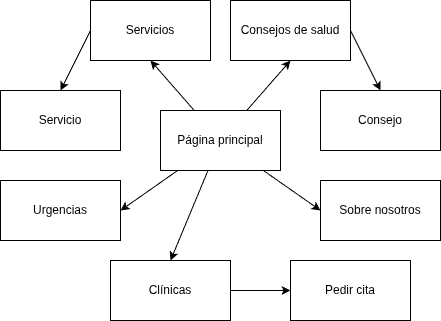
\includegraphics[width=\linewidth]{imgs_documento/inventarioDeContenido.png}
\caption{Inventario de contenido}
\end{figure}

\begin{table}[H]
\centering
\small
\setlength{\tabcolsep}{6pt}
\renewcommand{\arraystretch}{1.2}
\begin{tabularx}{\textwidth}{>{\raggedright\arraybackslash}p{3.6cm} >{\raggedright\arraybackslash}X >{\raggedright\arraybackslash}p{5.2cm}}
	\toprule
	\textbf{Páginas} & \textbf{Elementos clave a exponer} & \textbf{Objetivo del usuario} \\
	\midrule
	Página Principal &
	\begin{minipage}[t]{\linewidth}
		\begin{itemize}
			\item Buscador global de clínicas.
			\item Botón destacado de Urgencias.
			\item Accesos rápidos a Servicios y Consejos.
		\end{itemize}
	\end{minipage}
	& Acceder rápidamente a la información crítica o iniciar la navegación. \\
	\addlinespace
	Urgencias &
	\begin{minipage}[t]{\linewidth}
		\begin{itemize}
			\item Listado filtrado: solo clínicas abiertas ahora.
			\item Botones de llamada directa.
			\item Aviso de “Llamar antes de acudir”.
		\end{itemize}
	\end{minipage}
	& Obtener atención veterinaria inmediata sin fricción. \\
	\addlinespace
	Clínicas &
	\begin{minipage}[t]{\linewidth}
		\begin{itemize}
			\item Buscador por ubicación.
			\item Fichas con dirección y horario.
			\item Formulario emergente para reservar.
		\end{itemize}
	\end{minipage}
	& Localizar un centro y realizar la transacción (reservar cita). \\
	\addlinespace
	Servicios y servicio específico &
	\begin{minipage}[t]{\linewidth}
		\begin{itemize}
			\item Catálogo de tratamientos (Cirugía, Rayos X...).
			\item Páginas de detalle con explicación del procedimiento.
		\end{itemize}
	\end{minipage}
	& Informarse sobre qué tratamientos ofrece la franquicia. \\
	\addlinespace
	Consejos de Salud y consejo específico &
	\begin{minipage}[t]{\linewidth}
		\begin{itemize}
			\item Artículos educativos.
			\item Filtros por especie (Perros/Gatos/Otros animales).
		\end{itemize}
	\end{minipage}
	& Resolver dudas sobre cuidados y prevención (fidelización). \\
	\addlinespace
	Sobre Nosotros &
	\begin{minipage}[t]{\linewidth}
		\begin{itemize}
			\item Filosofía y valores (Sostenibilidad).
			\item Información corporativa.
		\end{itemize}
	\end{minipage}
	& Generar confianza y credibilidad en la marca. \\
	\bottomrule
\end{tabularx}
\caption{Inventario de contenidos, formato tabla}
\end{table}

\section{Storyboards}
\begin{figure}[H]
\centering
\rotatebox{90}{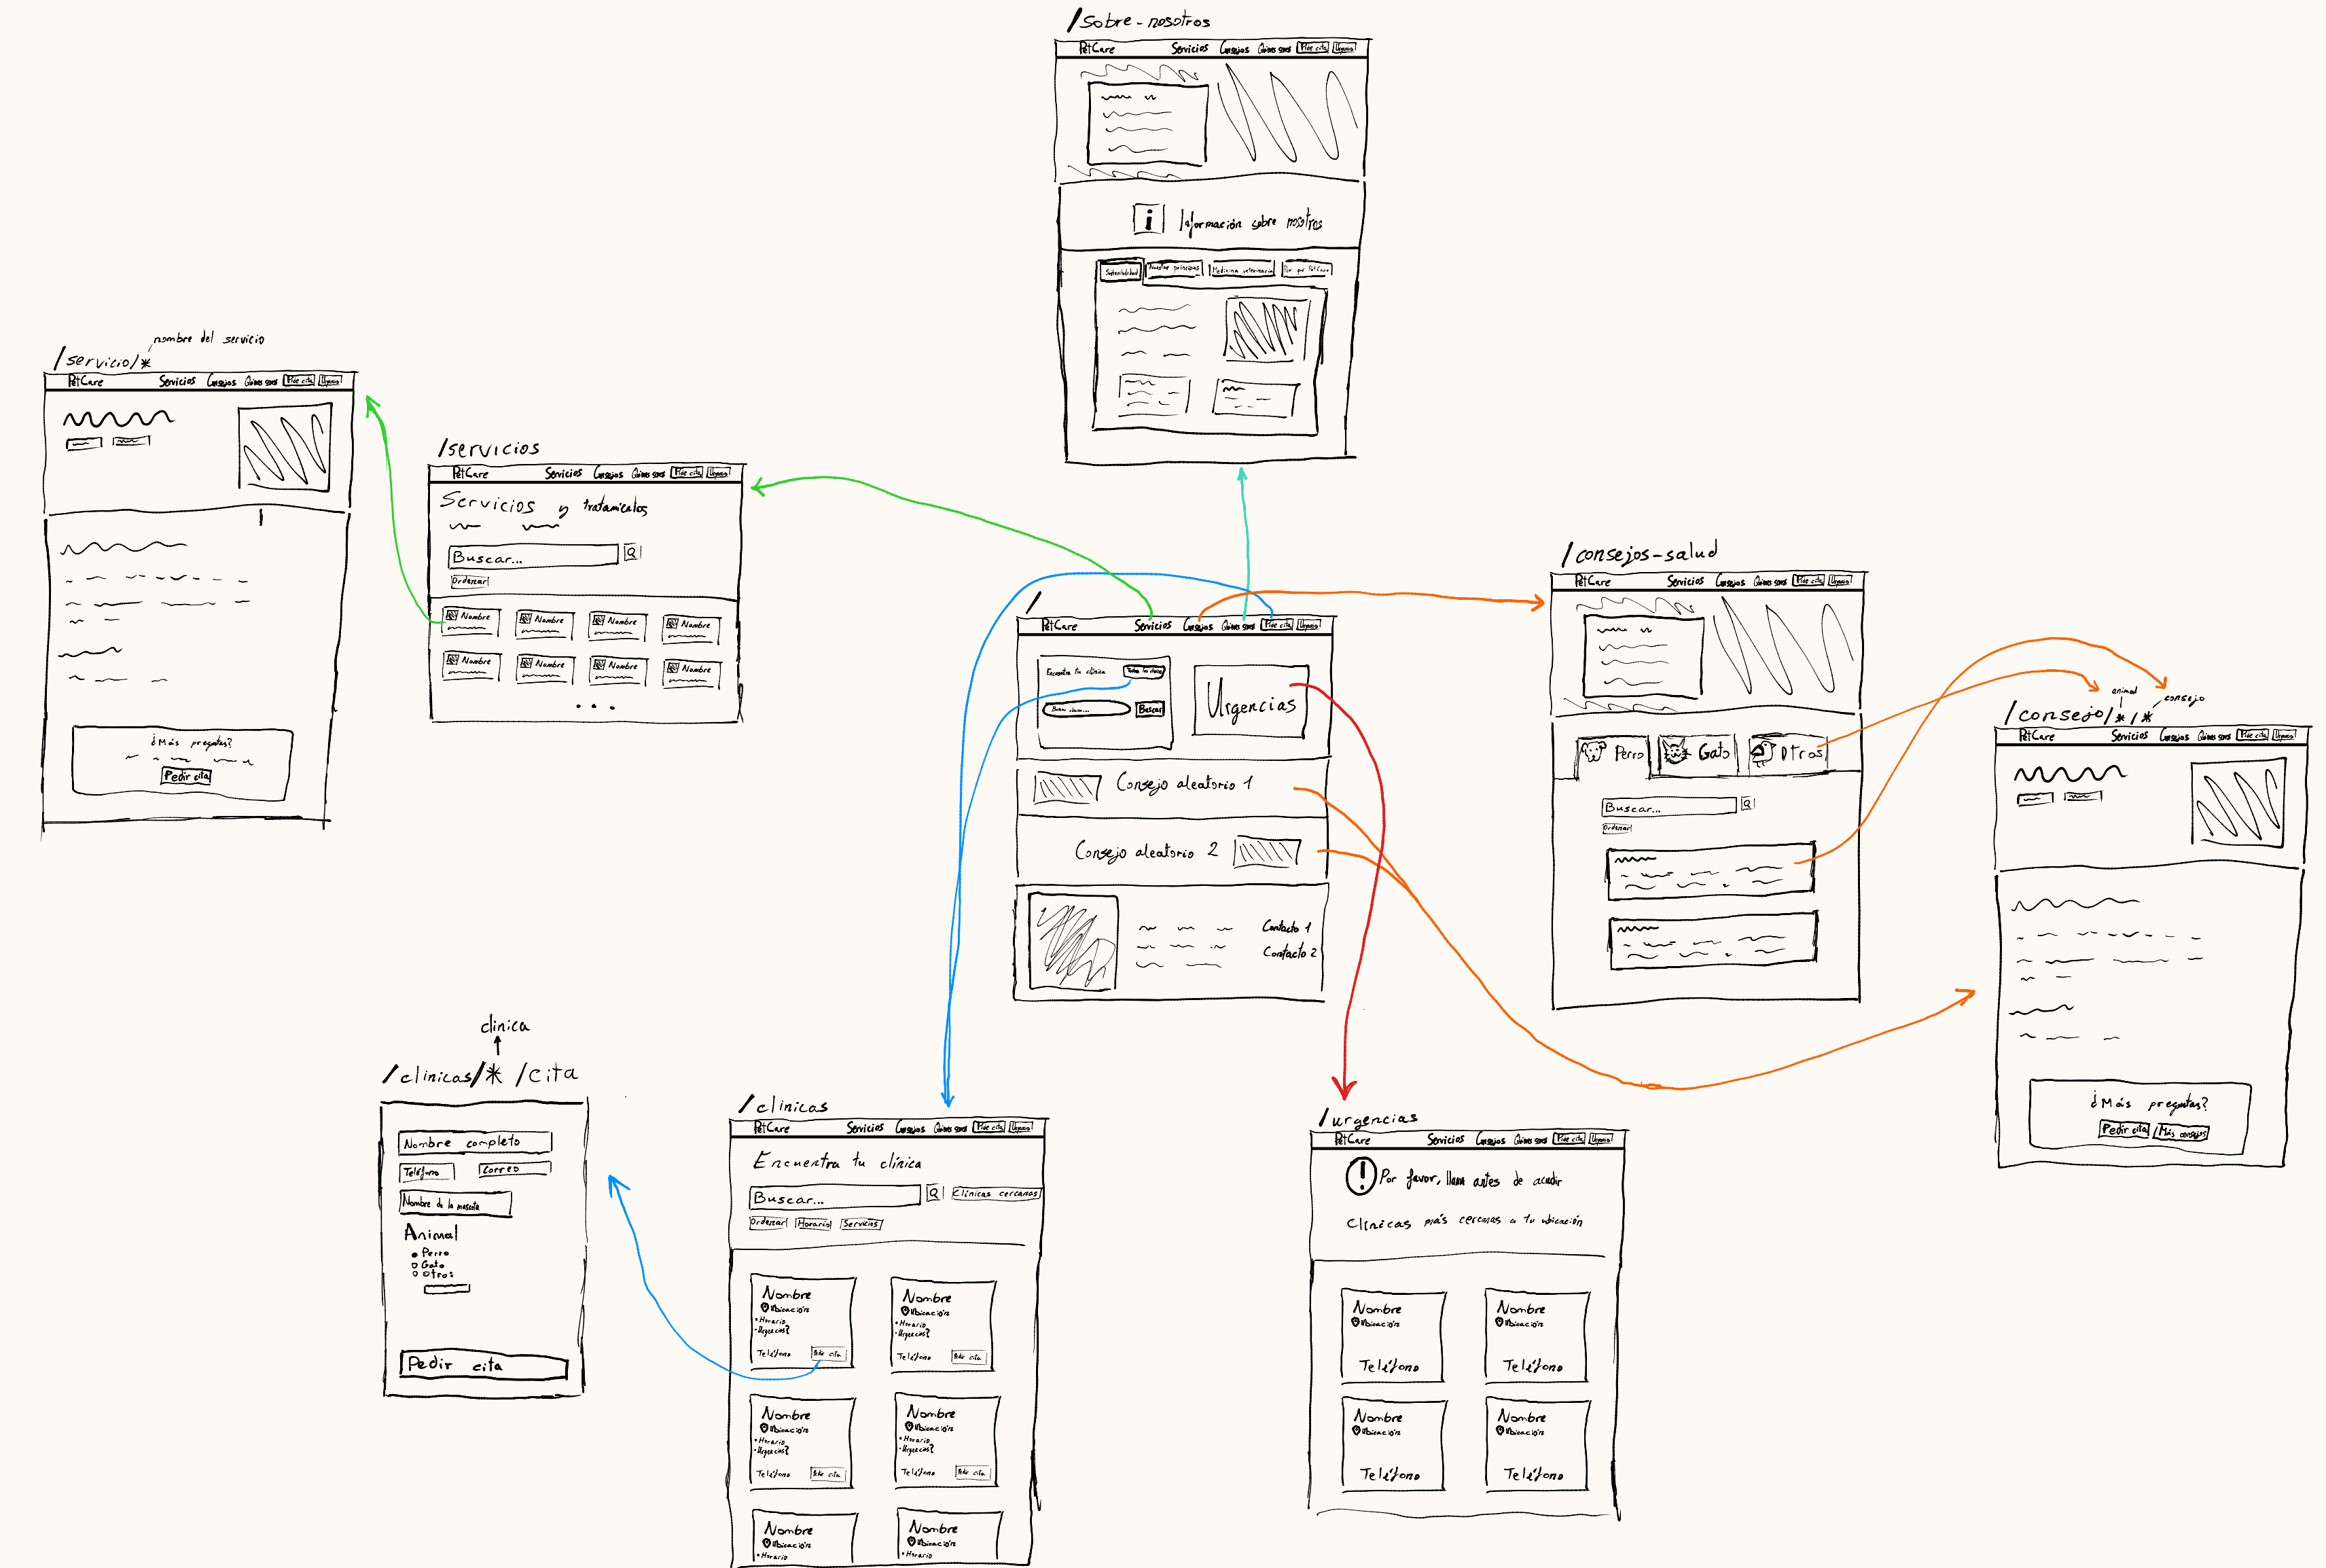
\includegraphics[width=\textheight,keepaspectratio]{imgs_documento/storyboard_daw.png}}
\caption{Storyboard}
\end{figure}

\section{Arquitectura de información}

\begin{figure}[H]
\centering
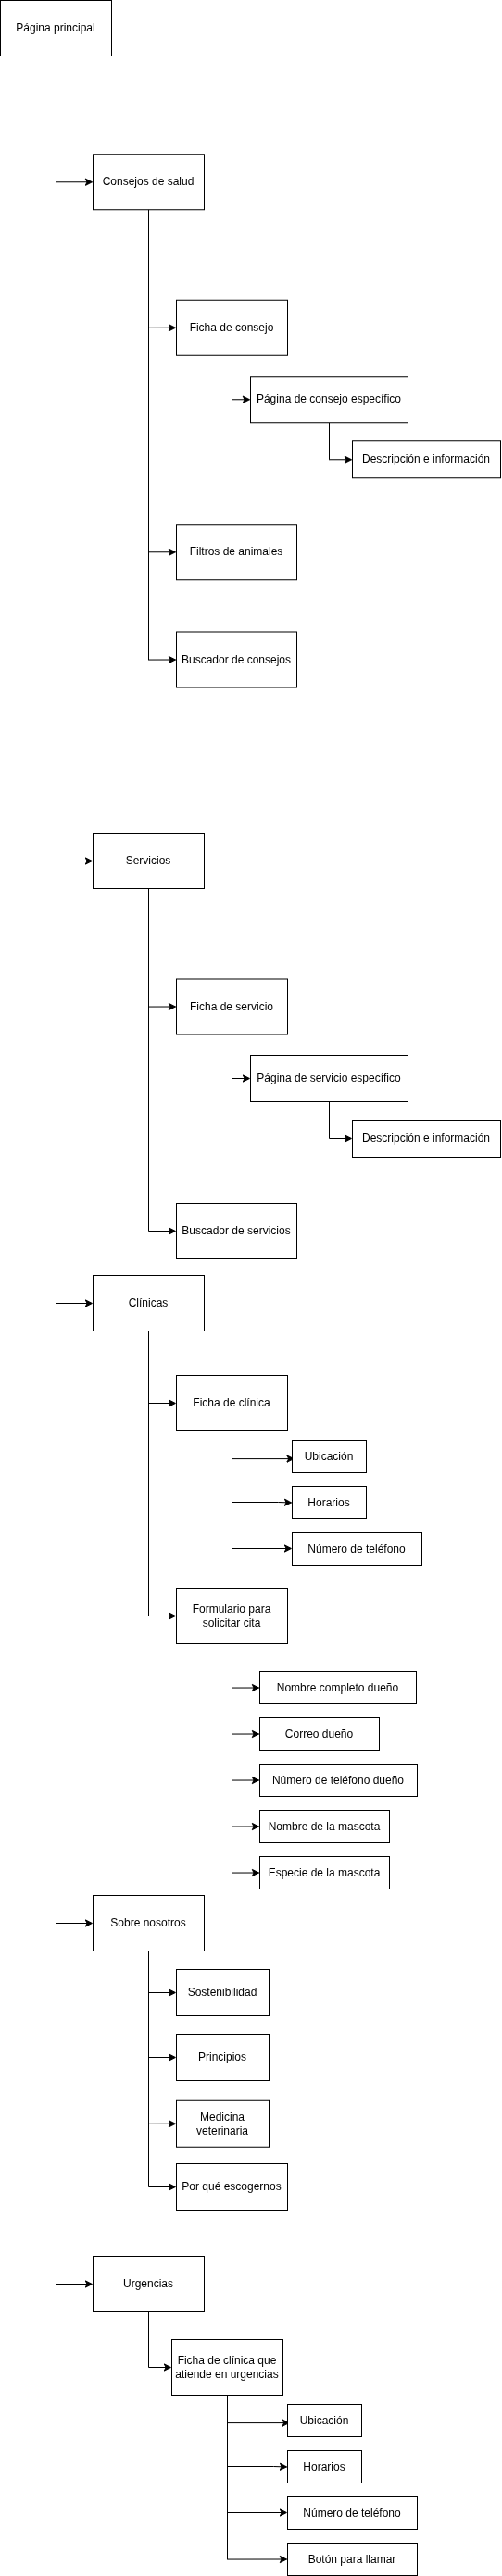
\includegraphics[ width=1.2\textwidth,height=0.95\textheight,keepaspectratio,clip,trim=0 1950 0 0]{imgs_documento/arquitecturaDeInformacion.png}
\caption{Arquitectura de información (1/3)}
\end{figure}

\clearpage

\begin{figure}[H]
\centering
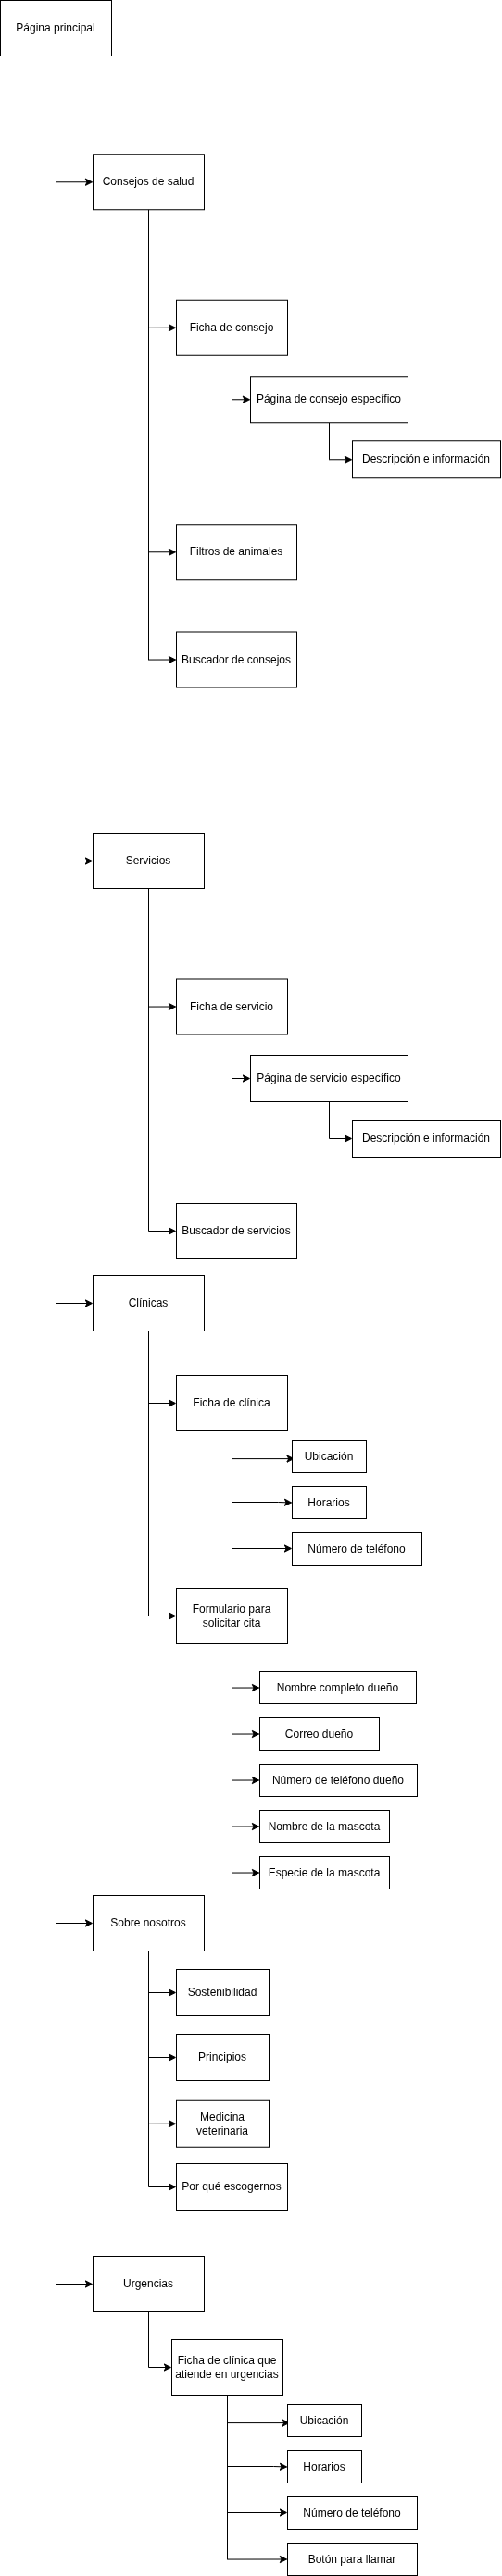
\includegraphics[width=1.2\textwidth,height=0.95\textheight,keepaspectratio,clip,trim=0 0 0 1407]{imgs_documento/arquitecturaDeInformacion.png}
\caption{Arquitectura de información (2/2)}
\end{figure}

\section{Mapa de navegación}

\begin{figure}[H]
\centering
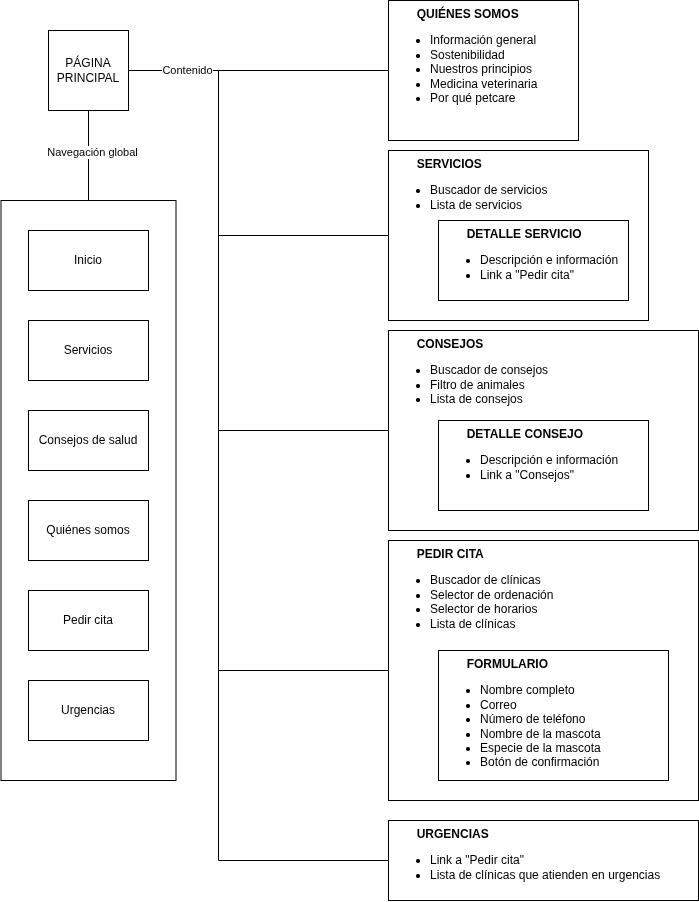
\includegraphics[width=\linewidth]{imgs_documento/mapaDeNavegacion.png}
\caption{Mapa de navegación}
\end{figure}

\section{Casos de uso abordados}

\begin{figure}[H]
\centering
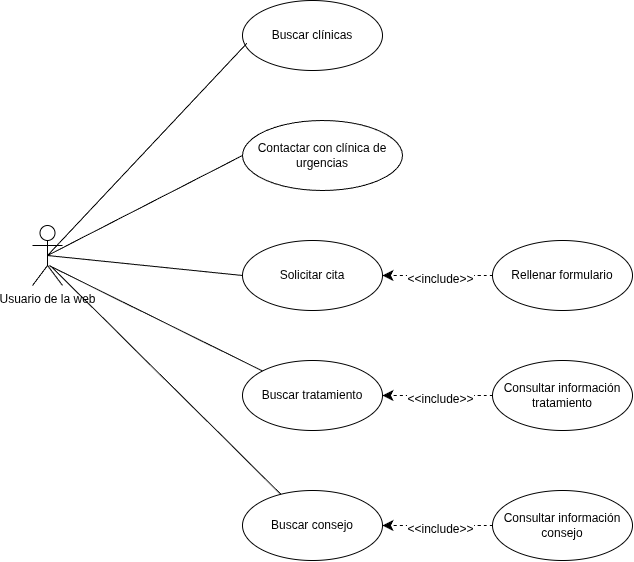
\includegraphics[width=\linewidth,height=0.95\textheight,keepaspectratio]{imgs_documento/casosDeUso_daw.png}
\caption{Casos de uso}
\end{figure}
\clearpage

\section{Guía de estilos y aspectos técnicos}

El diseño de visual de PetCare está fundamentado en proporcionar una estilización de la identidad y asociarse a la psicología del color sanitaria priorizando unos tonos más pasteles, reduciendo la posibilidad de fatiga visual y transmitiendo calma. Se reservan colores más saturados únicamente para las llamadas a acción para guiar la atención del usuario, como sucede por ejemplo en la página principal con el botón grande de “Urgencias”.

\subsection{Paleta de colores}

Se definió un esquema cromático dividido en tres categorías funcionales:

\subsubsection{Colores base}

\begin{itemize}
\item \#ADB2D4: Usado como acento primario, para estados de selección, resaltados de foco y filtros activos.
\item \#D5D8EB: Variante m\u00e1s clara del acento primario, empleada en sombras suaves y fondos de elementos interactivos en reposo.
\item \#C7D9DD: Utilizado en fondos con degradado suave.
\item \#D5E5D5: Aplicado en fondos de sección alternativos y badges (etiquetas) de categoría.
\item \#EEF1DA: Fondos cálidos para secciones informativas ligeras.
\end{itemize}

\subsubsection{Colores de llamada a la acción}

\begin{itemize}
\item \#EF5A6F: Color Crítico. Reservado exclusivamente para el botón flotante y avisos de “Urgencias”.
\item \#7B82A8: Botones de acción principal (CTA), como “Pedir cita” o “Buscar”.
\item \#88C9A1: Acciones secundarias o de confirmación (ej: “Ver clínicas cercanas”).
\end{itemize}

\subsubsection{Colores para tipografías y tonos neutros}

\begin{itemize}
\item Texto Principal (\#2A2D3F): Tono Dark Charcoal para títulos y lectura principal.
\item Texto Secundario (\#4A4a5E): Tono Medium Gray para cuerpo de texto, descripciones y etiquetas.
\item Fondos Neutros: Blanco puro (\#FFFFFF) para tarjetas y contenedores; Off-white (\#F9FAFB) para fondos de inputs en formularios.
\end{itemize}

\subsection{Tipografías}

Se utilizan principalmente dos familias tipográficas de Google Fonts para distinguir claramente la estructura de la página.

Para Títulos: Poppins (Sans-serif geométrica)

Peso: Utilizada exclusivamente en seminegrita.

Propósito: Aportar modernidad y estilizar.

Aplicación: Encabezados h1, h2, h3 y títulos de tarjetas.

Para Cuerpo: Inter (Sans-serif humanista)

Pesos: Utilizada en diversos pesos.

Propósito: Aportar mayor legibilidad independientemente del tamaño de la pantalla del dispositivo.

Aplicación: Párrafos, descripciones, etiquetas de formularios y textos de botones.

\subsection{Identidad visual en el diseño}

Como rasgo relativamente distintivo de la interfaz de usuario se han definido múltiples bordes asimétricos suavizando la rigidez de una maquetación con bordes más afilados.

\section{Interfaces}

\subsection{Bocetos a mano alzada}

\begin{figure}[H]
\centering
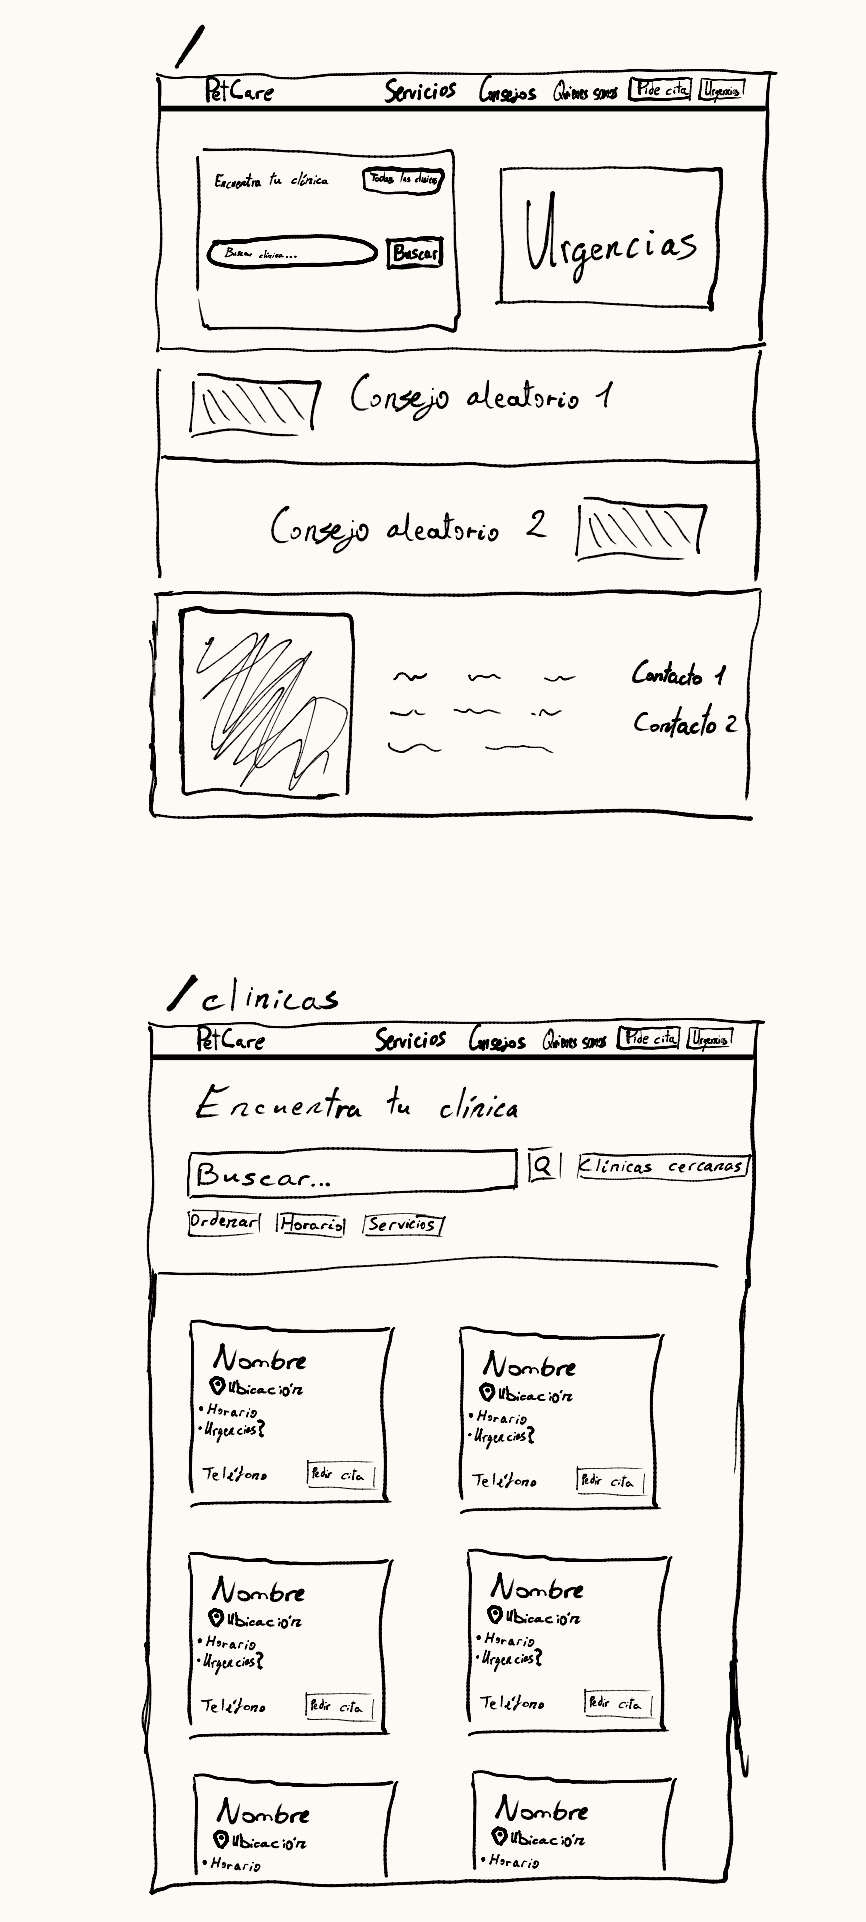
\includegraphics[width=\linewidth,height=0.95\textheight,keepaspectratio]{imgs_documento/bocetos1.png}
\caption{Bocetos (1/5)}
\end{figure}
\clearpage

\begin{figure}[H]
\centering
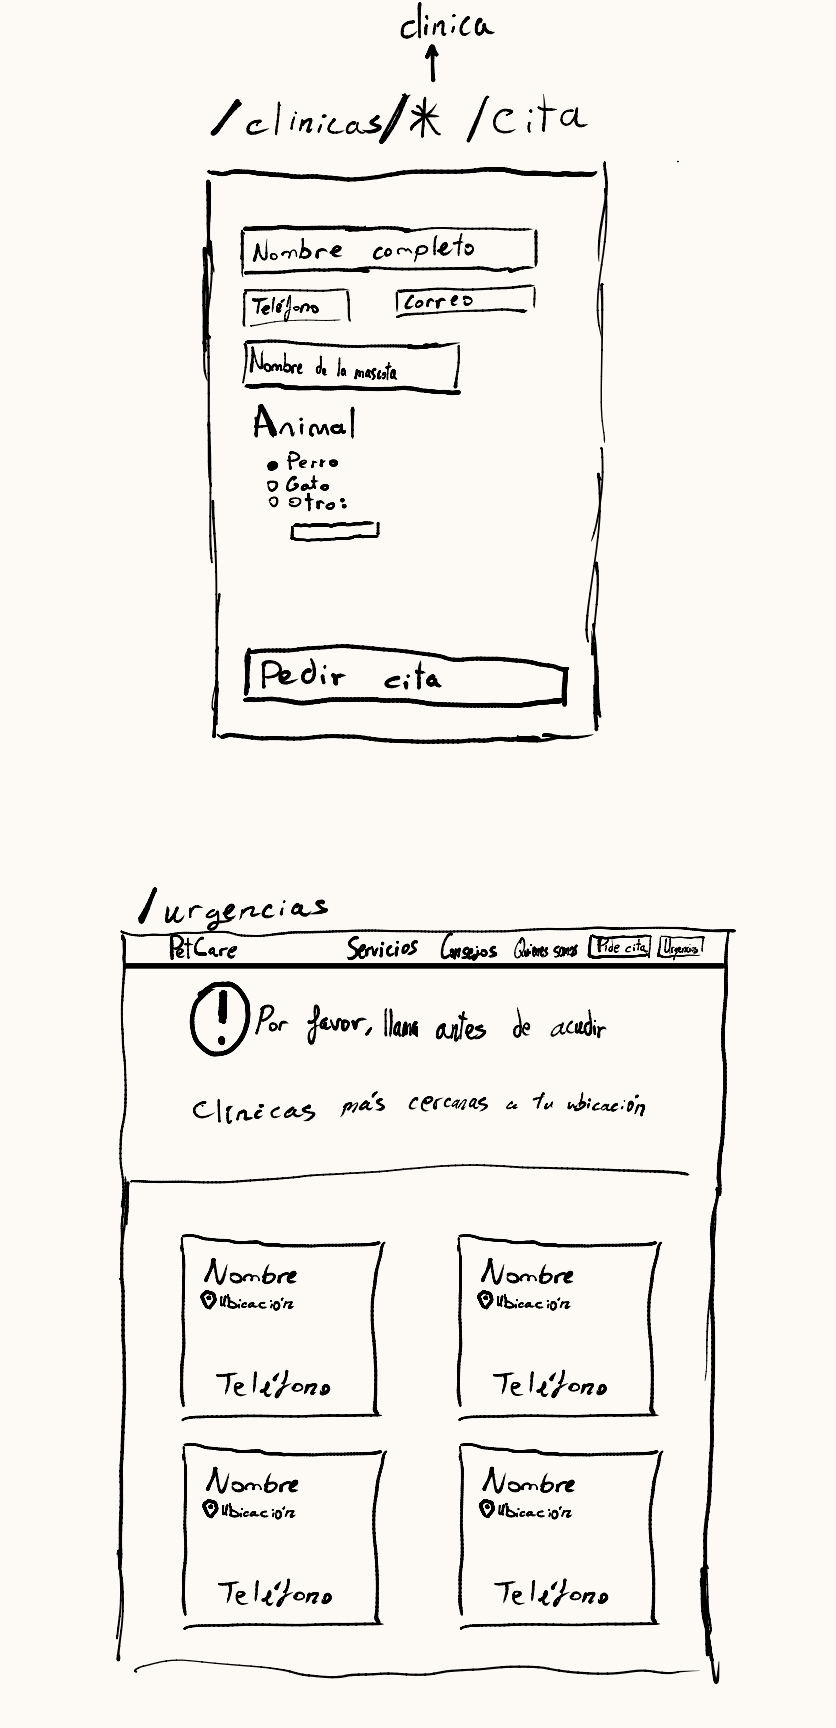
\includegraphics[width=\linewidth,height=0.95\textheight,keepaspectratio]{imgs_documento/bocetos2.png}
\caption{Bocetos (2/5)}
\end{figure}
\clearpage

\begin{figure}[H]
\centering
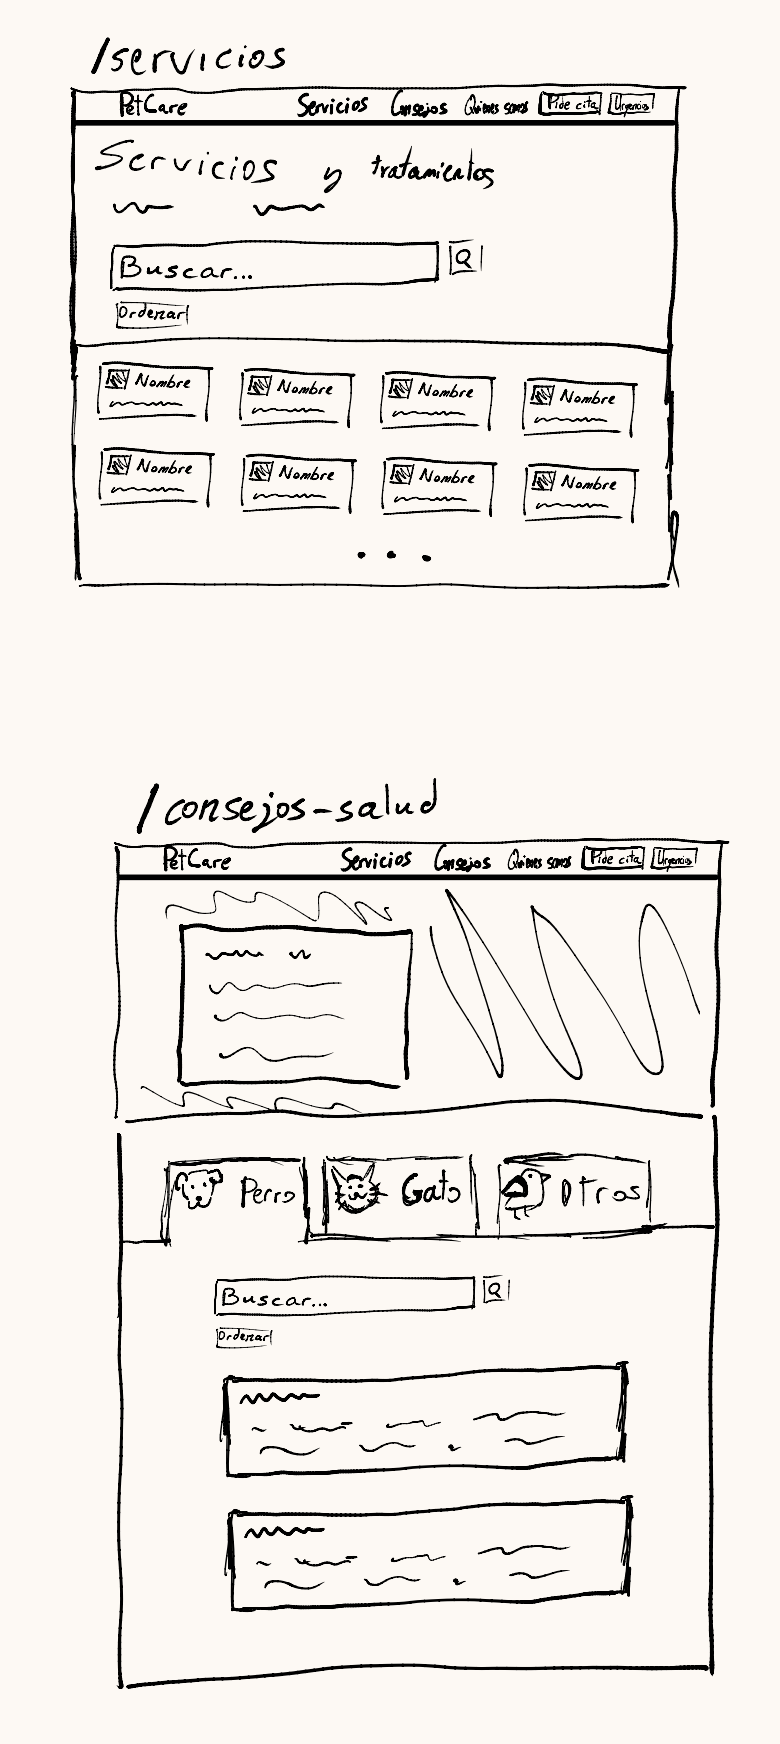
\includegraphics[width=\linewidth,height=0.95\textheight,keepaspectratio]{imgs_documento/bocetos3.png}
\caption{Bocetos (3/5)}
\end{figure}
\clearpage

\begin{figure}[H]
\centering
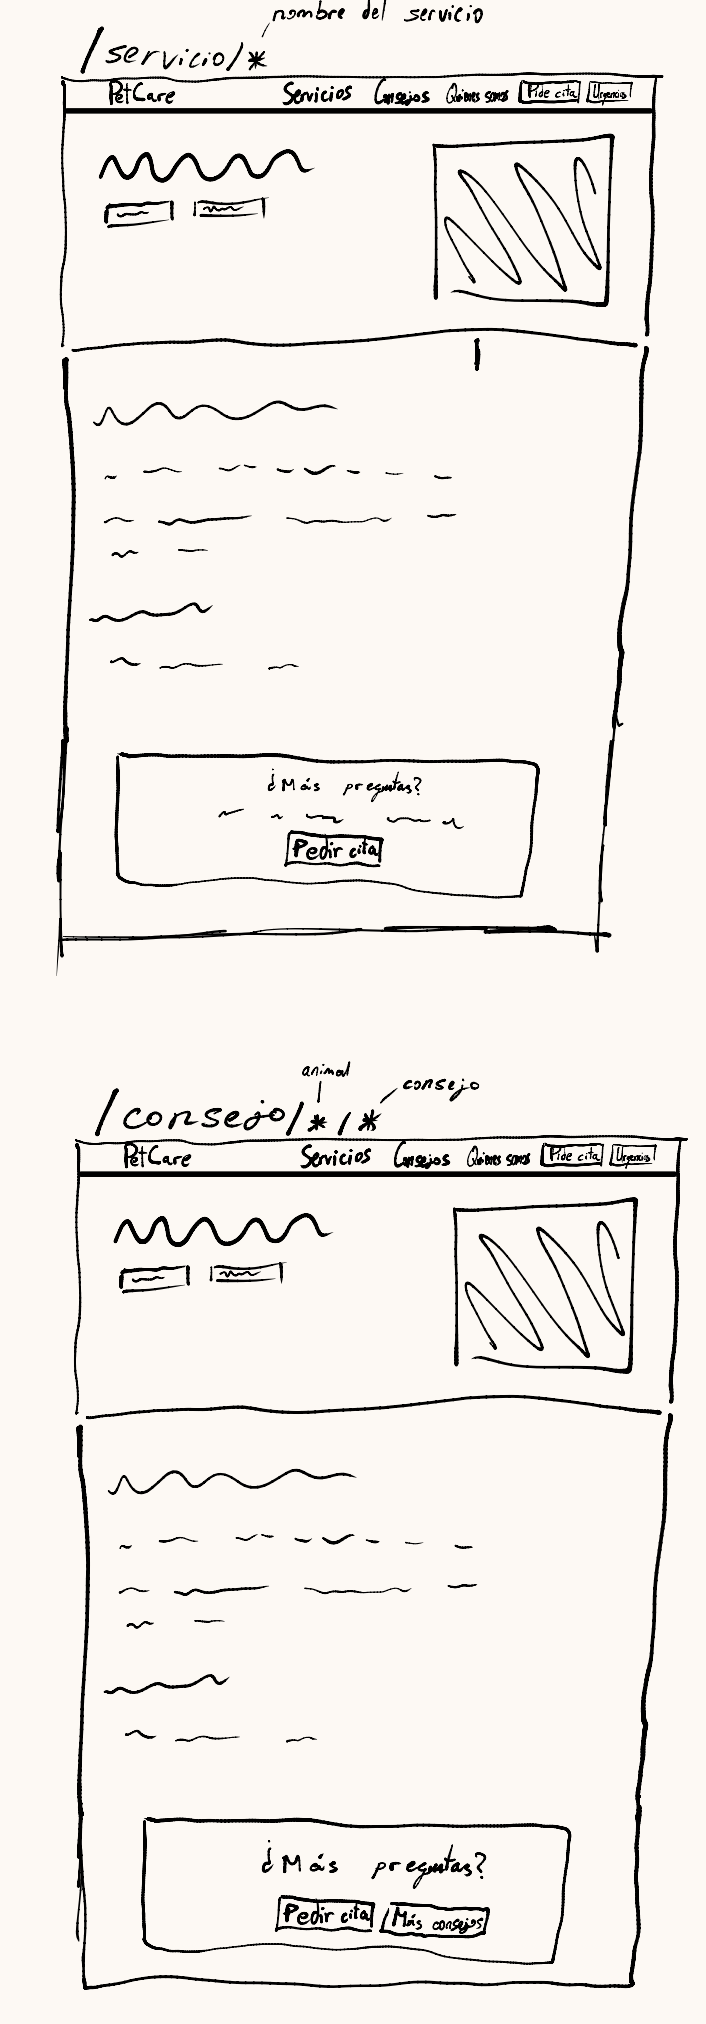
\includegraphics[width=\linewidth,height=0.95\textheight,keepaspectratio]{imgs_documento/bocetos4.png}
\caption{Bocetos (4/5)}
\end{figure}
\clearpage

\begin{figure}[H]
\centering
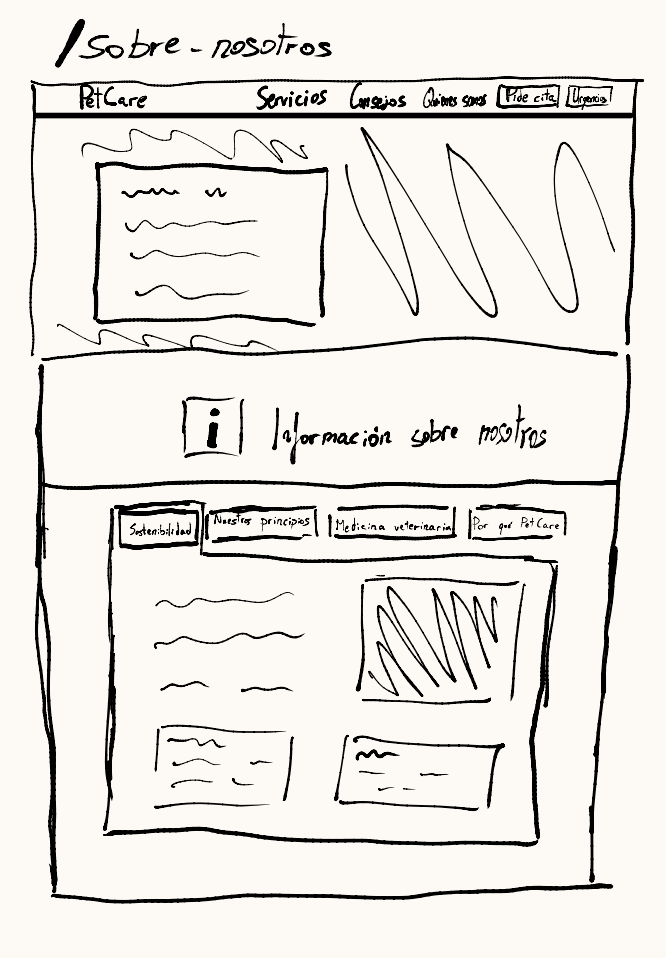
\includegraphics[width=\linewidth,height=0.95\textheight,keepaspectratio]{imgs_documento/bocetos5.png}
\caption{Bocetos (5/5)}
\end{figure}
\clearpage

\subsection{Wireframes}

\subsubsection{Página principal}
\begin{figure}[H]
\centering
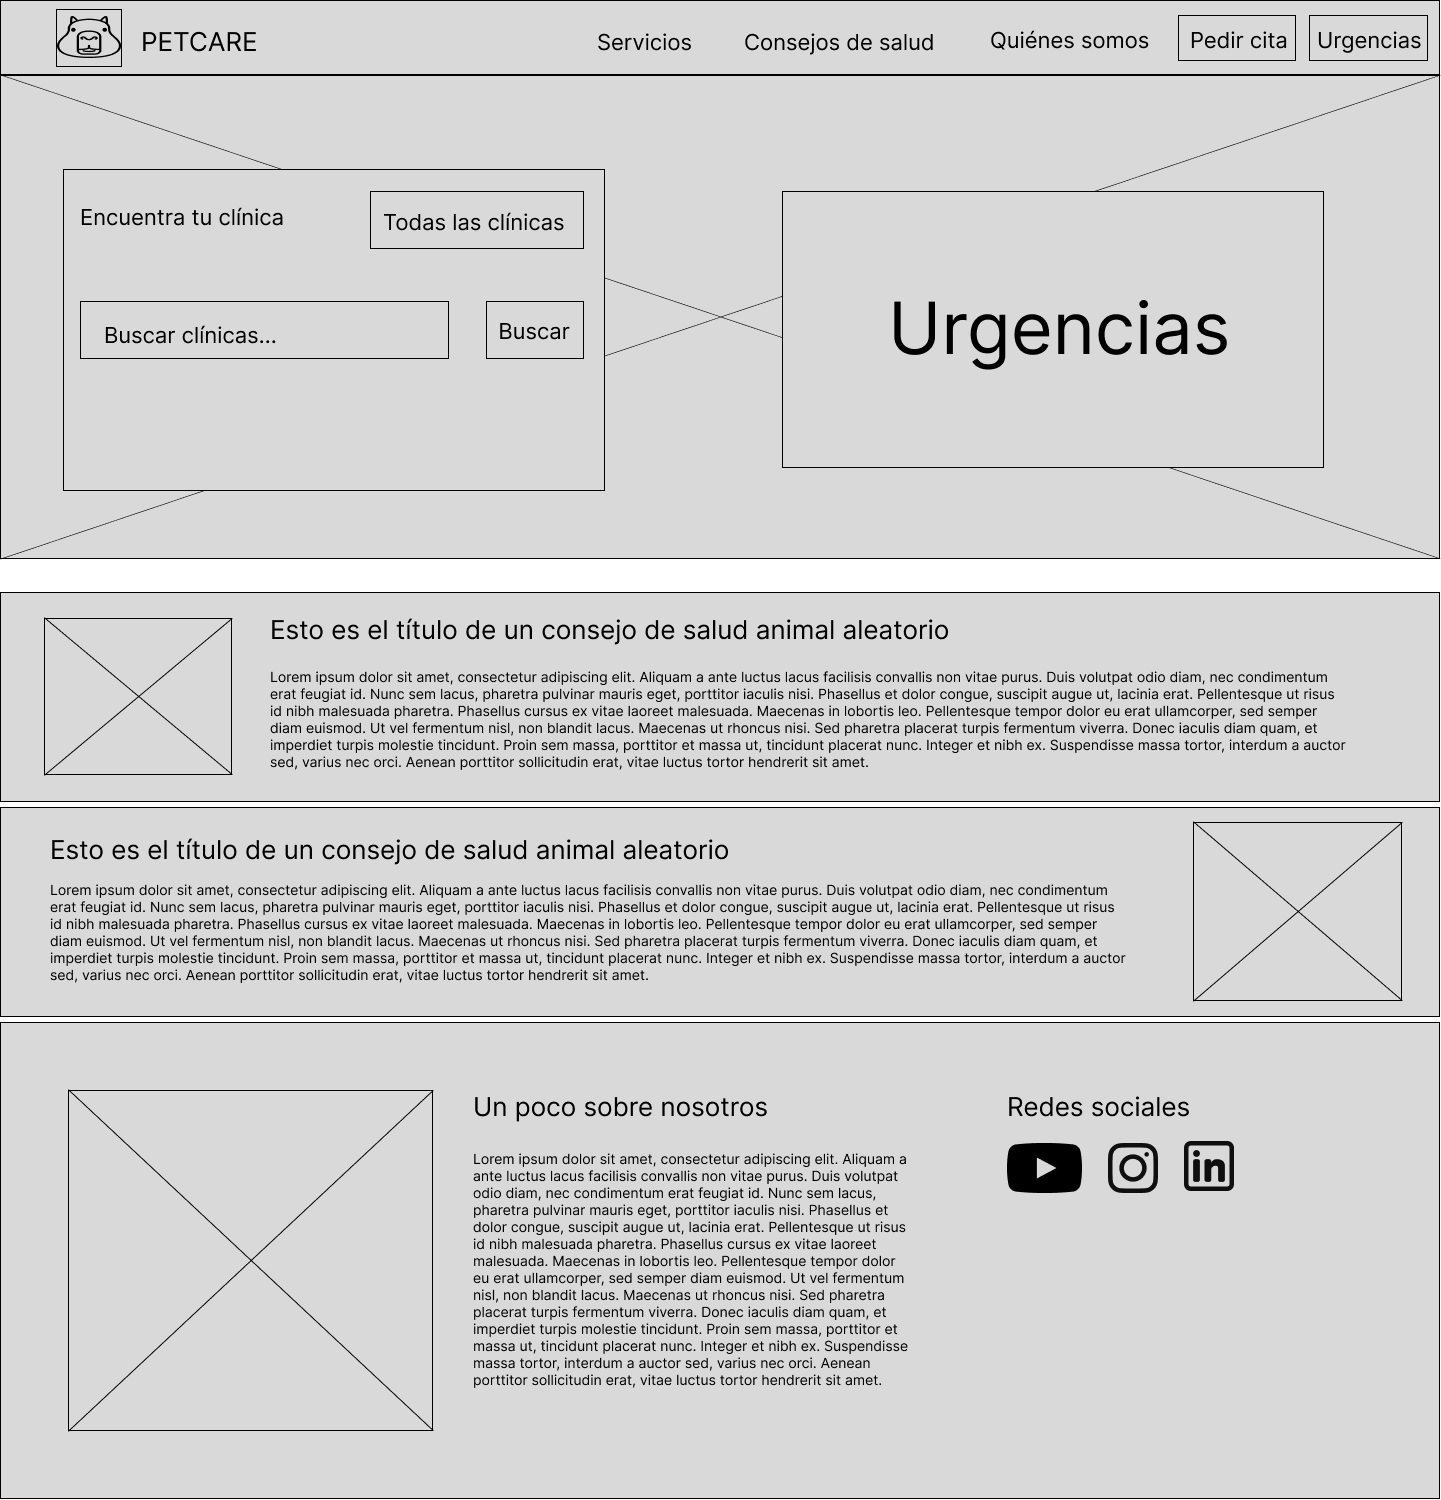
\includegraphics[width=\linewidth,height=0.95\textheight,keepaspectratio]{imgs_documento/wireframes/Wireframe_home.png}
\caption{Wireframe de página principal}
\end{figure}
\clearpage

\subsubsection{Clínicas}
\begin{figure}[H]
\centering
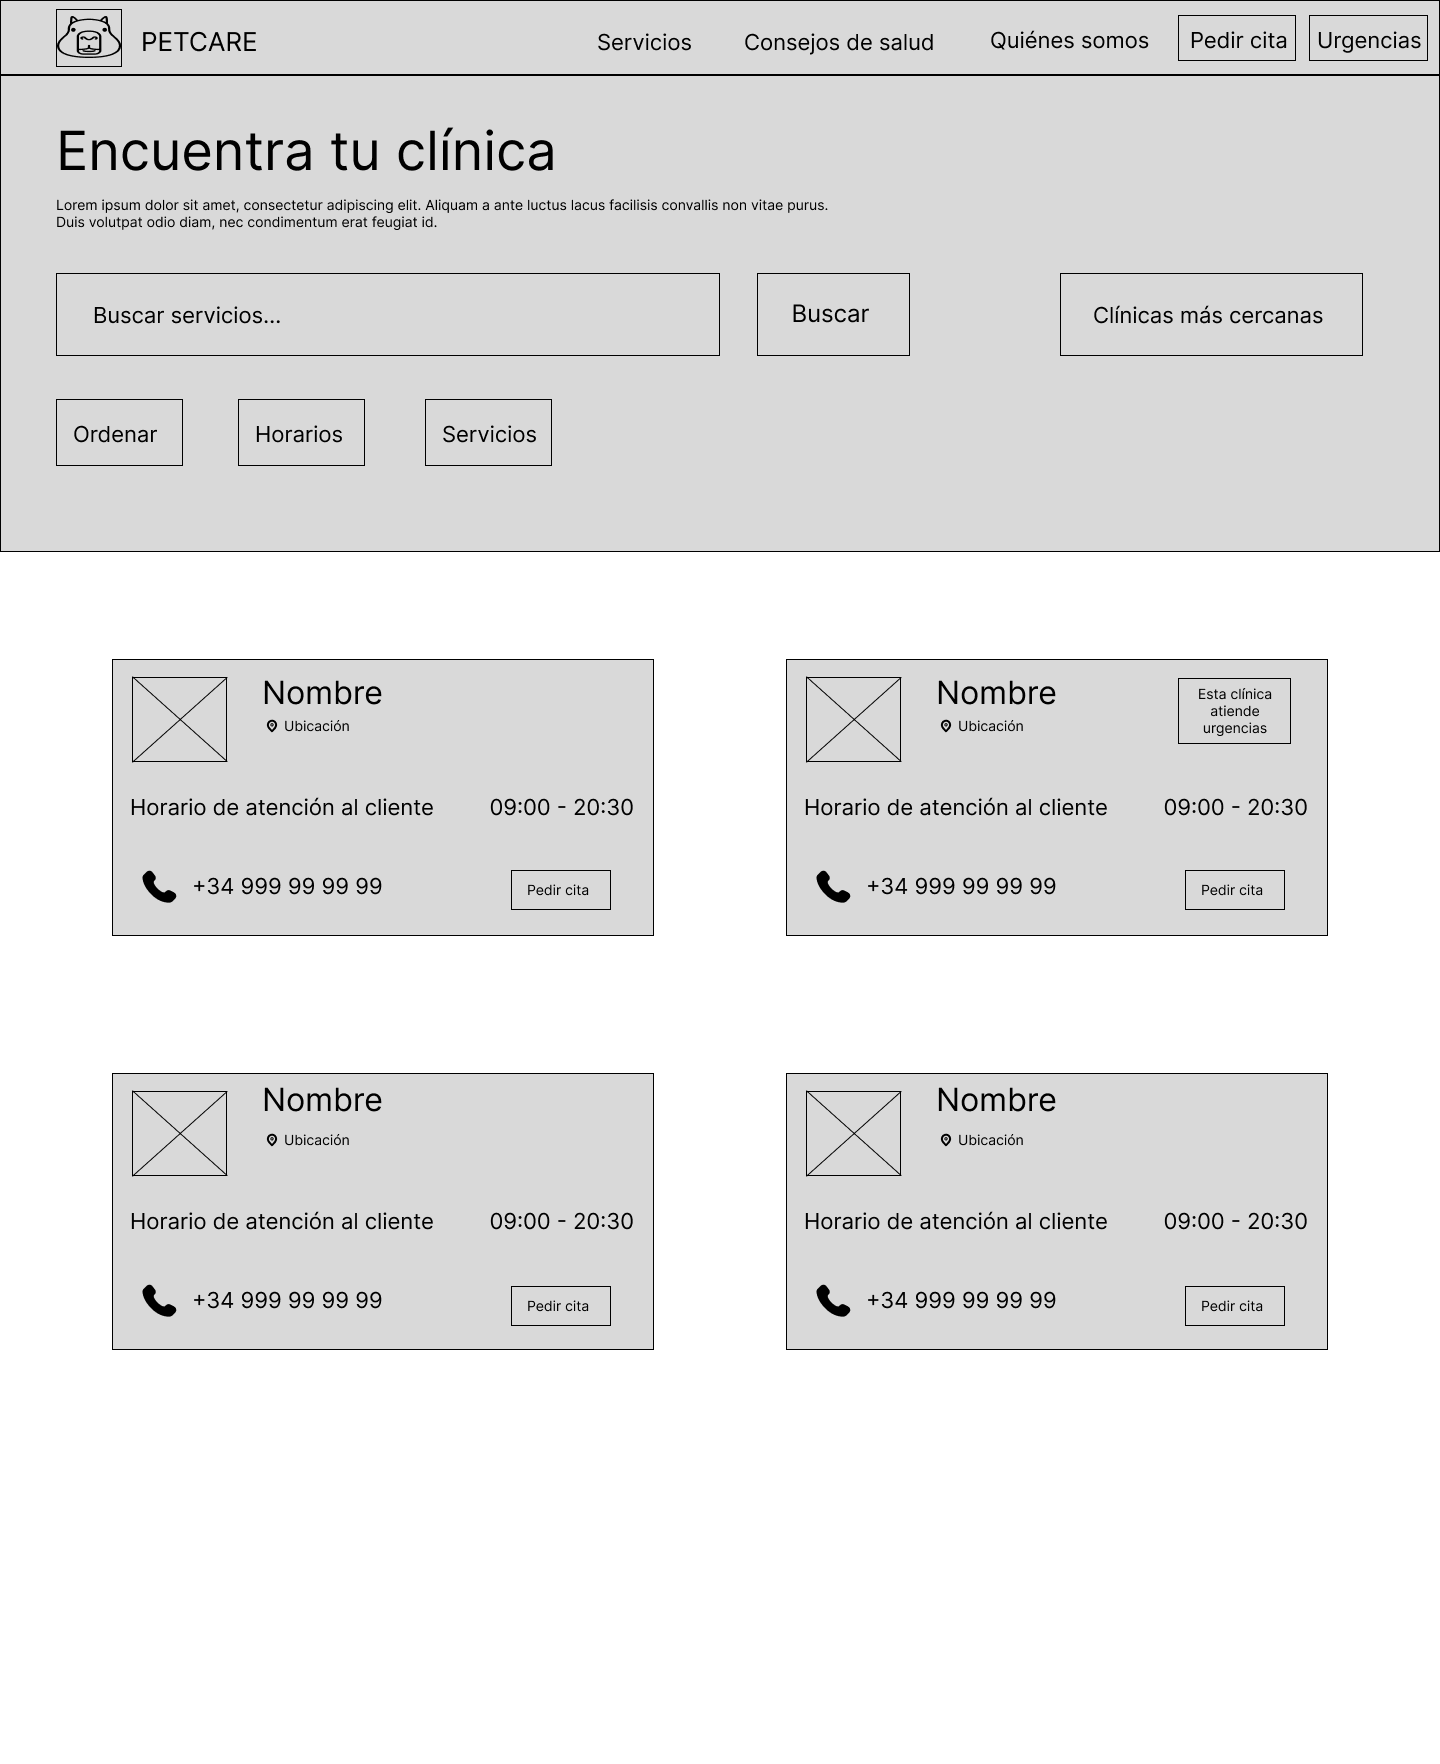
\includegraphics[width=\linewidth,height=0.95\textheight,keepaspectratio]{imgs_documento/wireframes/Wireframe_clinicas.png}
\caption{Wireframe de página de clínicas}
\end{figure}
\clearpage

\subsubsection{Urgencias}
\begin{figure}[H]
\centering
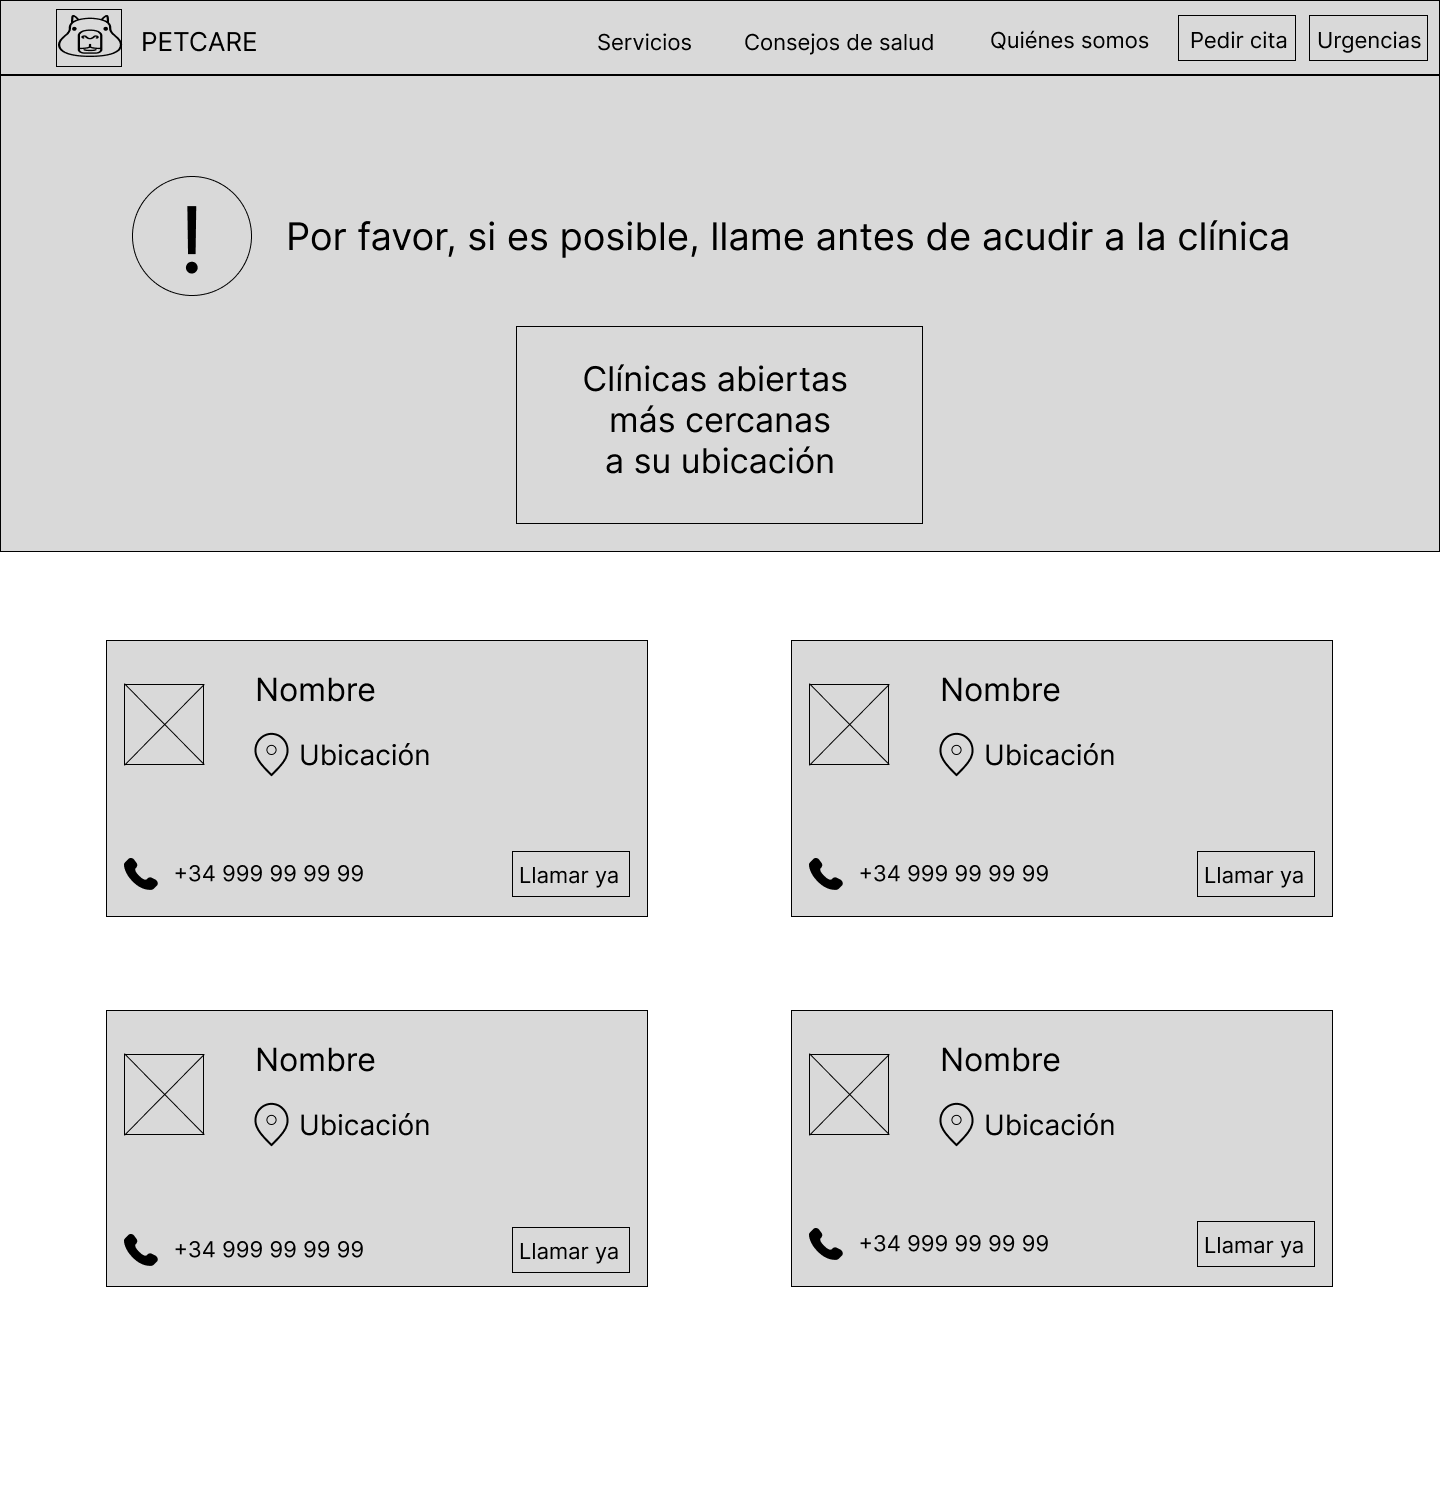
\includegraphics[width=\linewidth,height=0.95\textheight,keepaspectratio]{imgs_documento/wireframes/Wireframe_urgencias.png}
\caption{Wireframe de página de urgencias}
\end{figure}
\clearpage

\subsubsection{Servicios y tratamientos}
\begin{figure}[H]
\centering
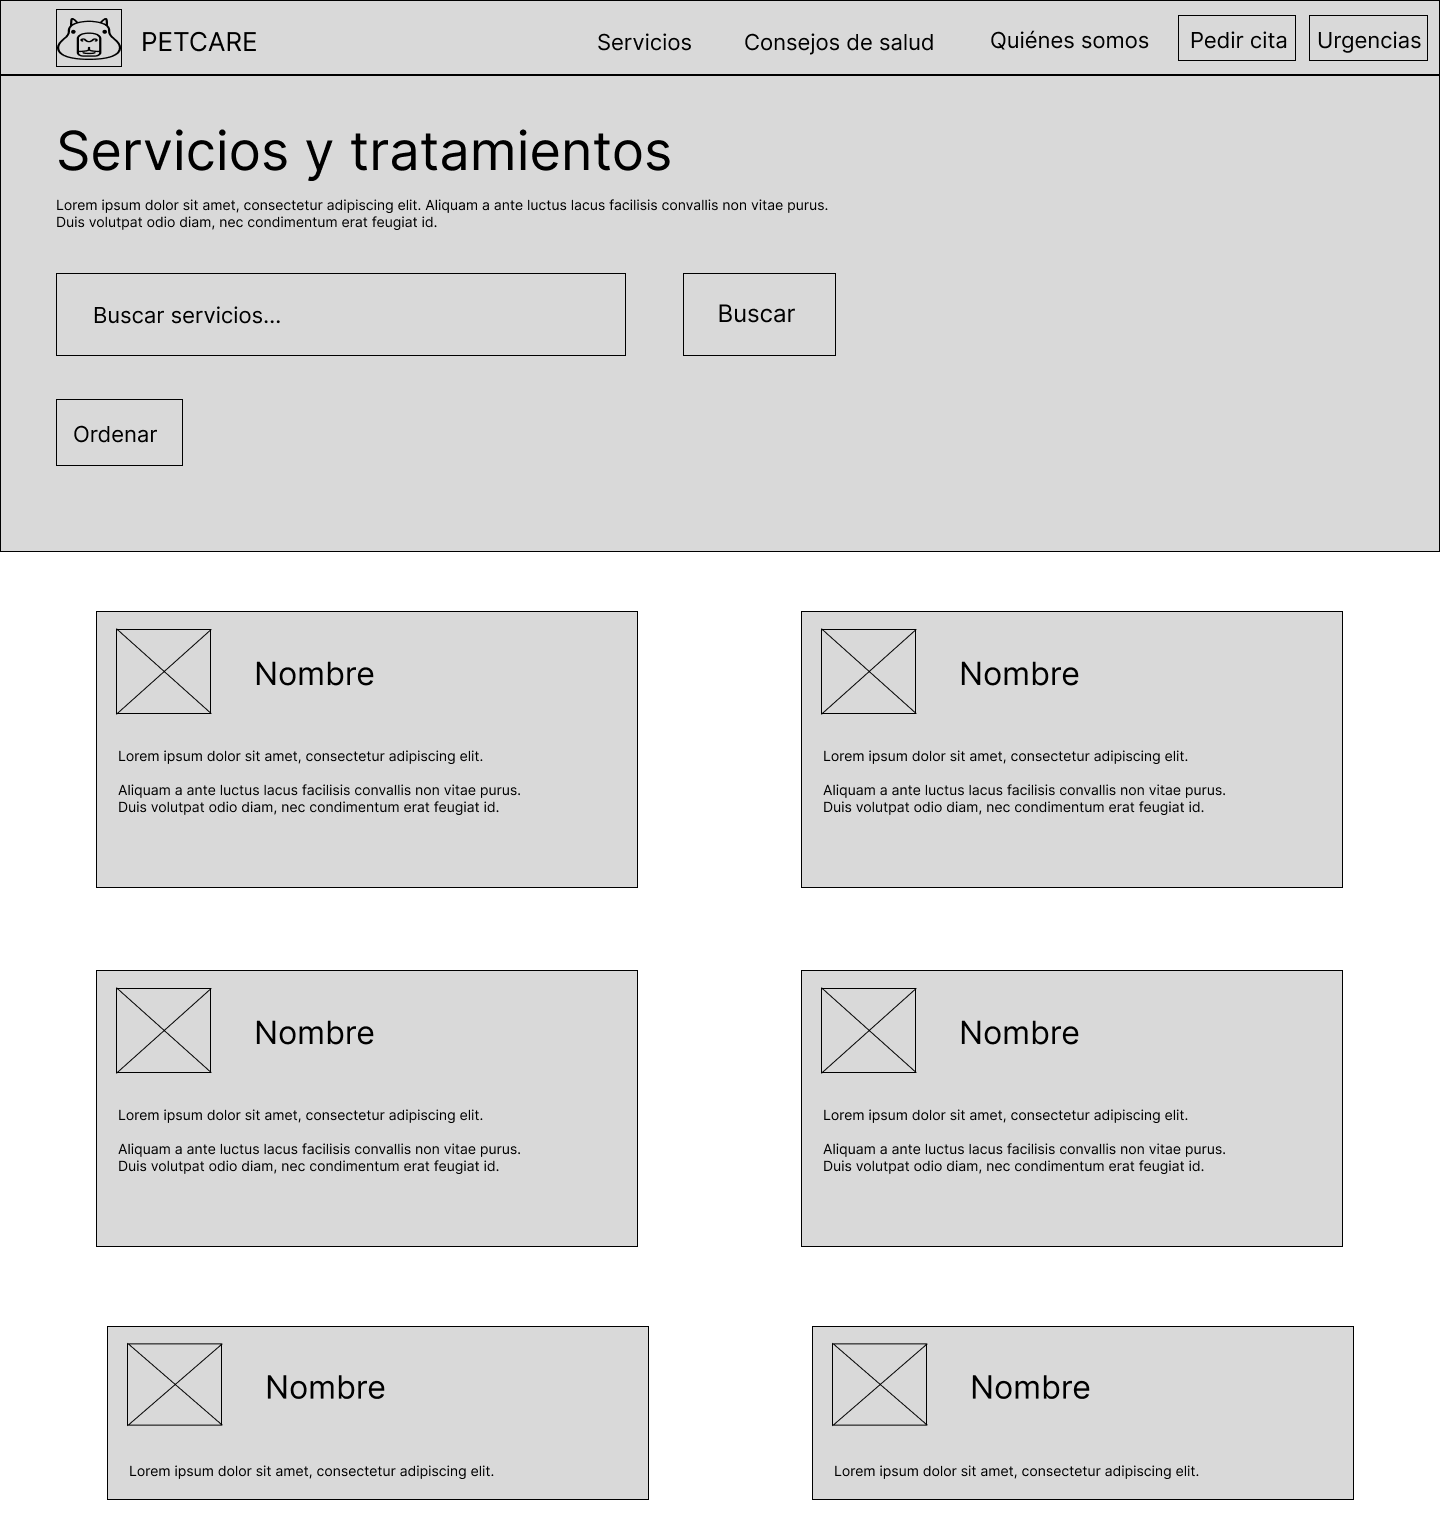
\includegraphics[width=\linewidth,height=0.95\textheight,keepaspectratio]{imgs_documento/wireframes/Wireframe-ServiciosYTratamientos.png}
\caption{Wireframe de página de servicios y tratamientos}
\end{figure}
\clearpage

\subsubsection{Servicio específico}
\begin{figure}[H]
\centering
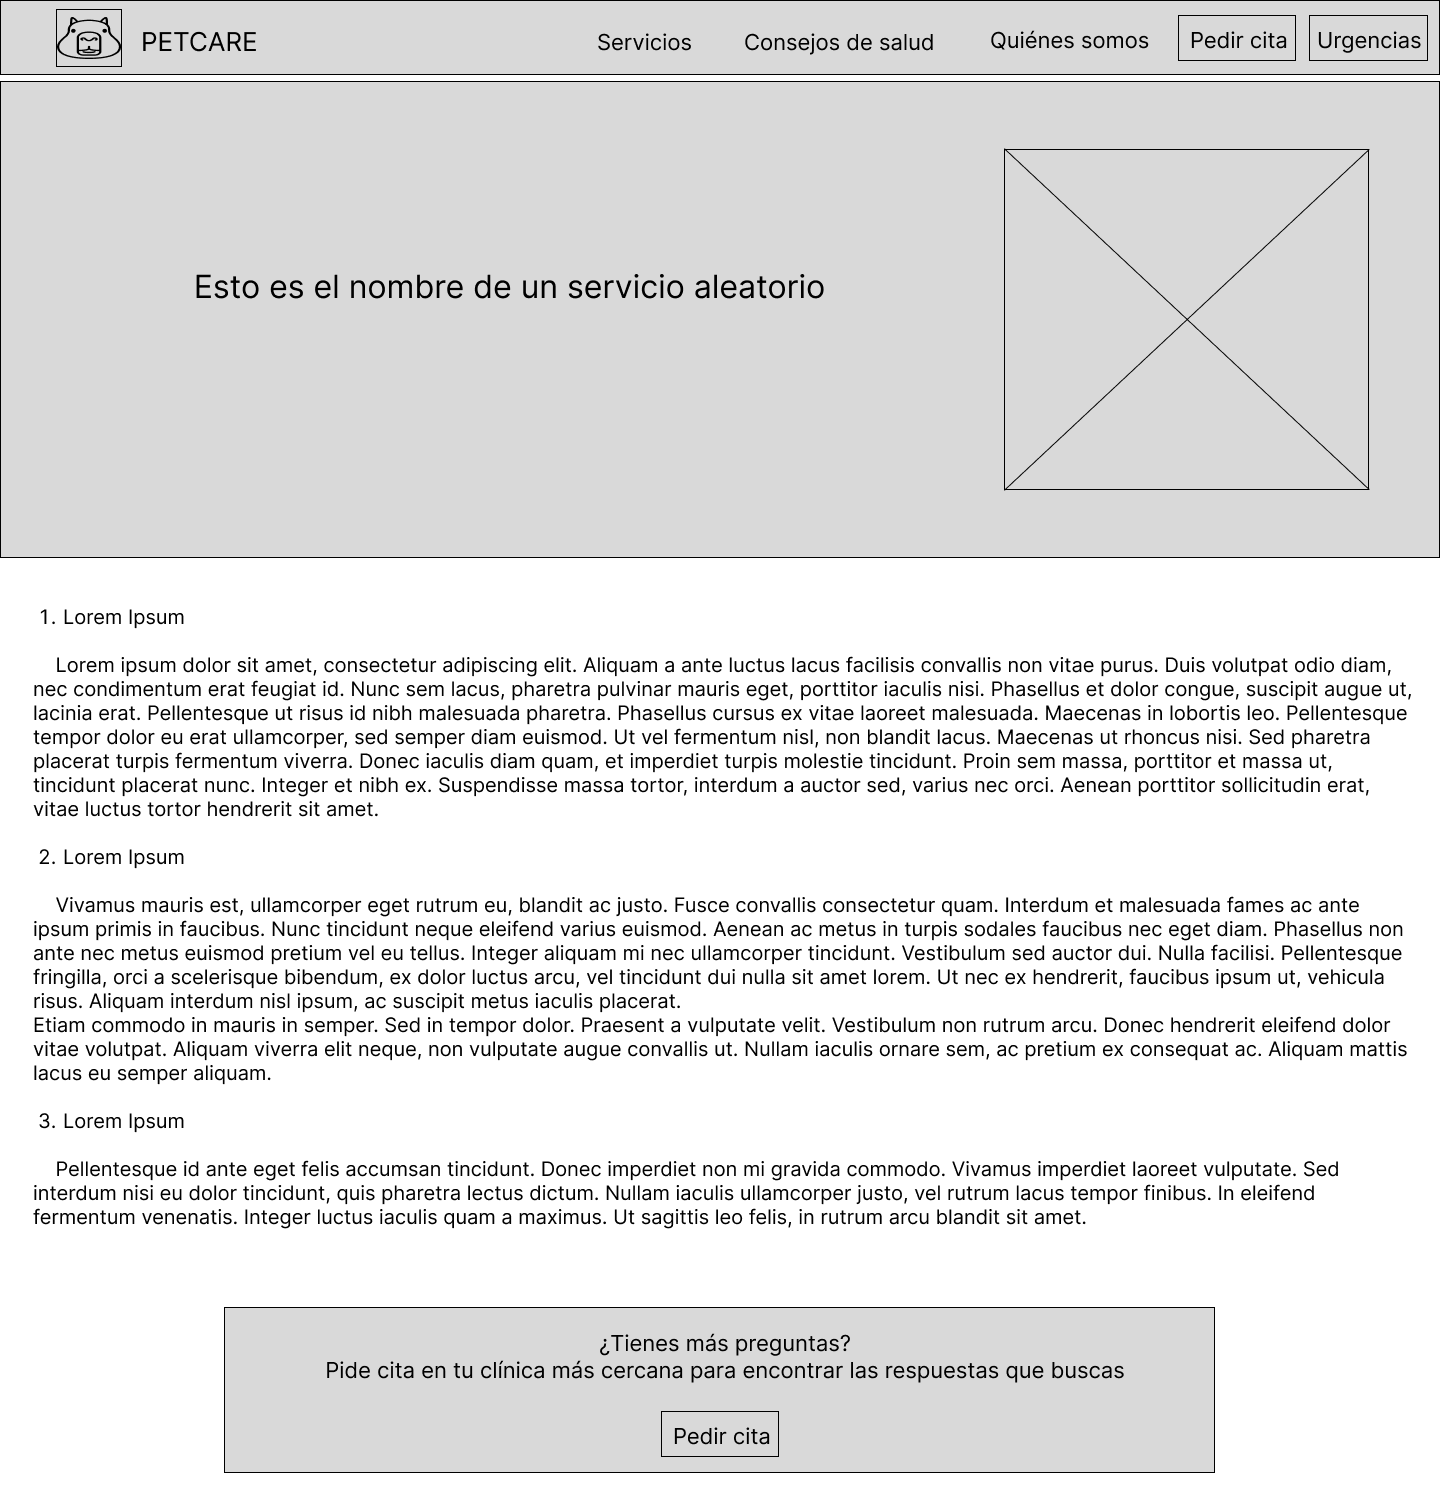
\includegraphics[width=\linewidth,height=0.95\textheight,keepaspectratio]{imgs_documento/wireframes/Wireframe_ServicioConcreto.png}
\caption{Wireframede la página de un servicio específico}
\end{figure}
\clearpage

\subsubsection{Sobre nosotros}
\begin{figure}[H]
\centering
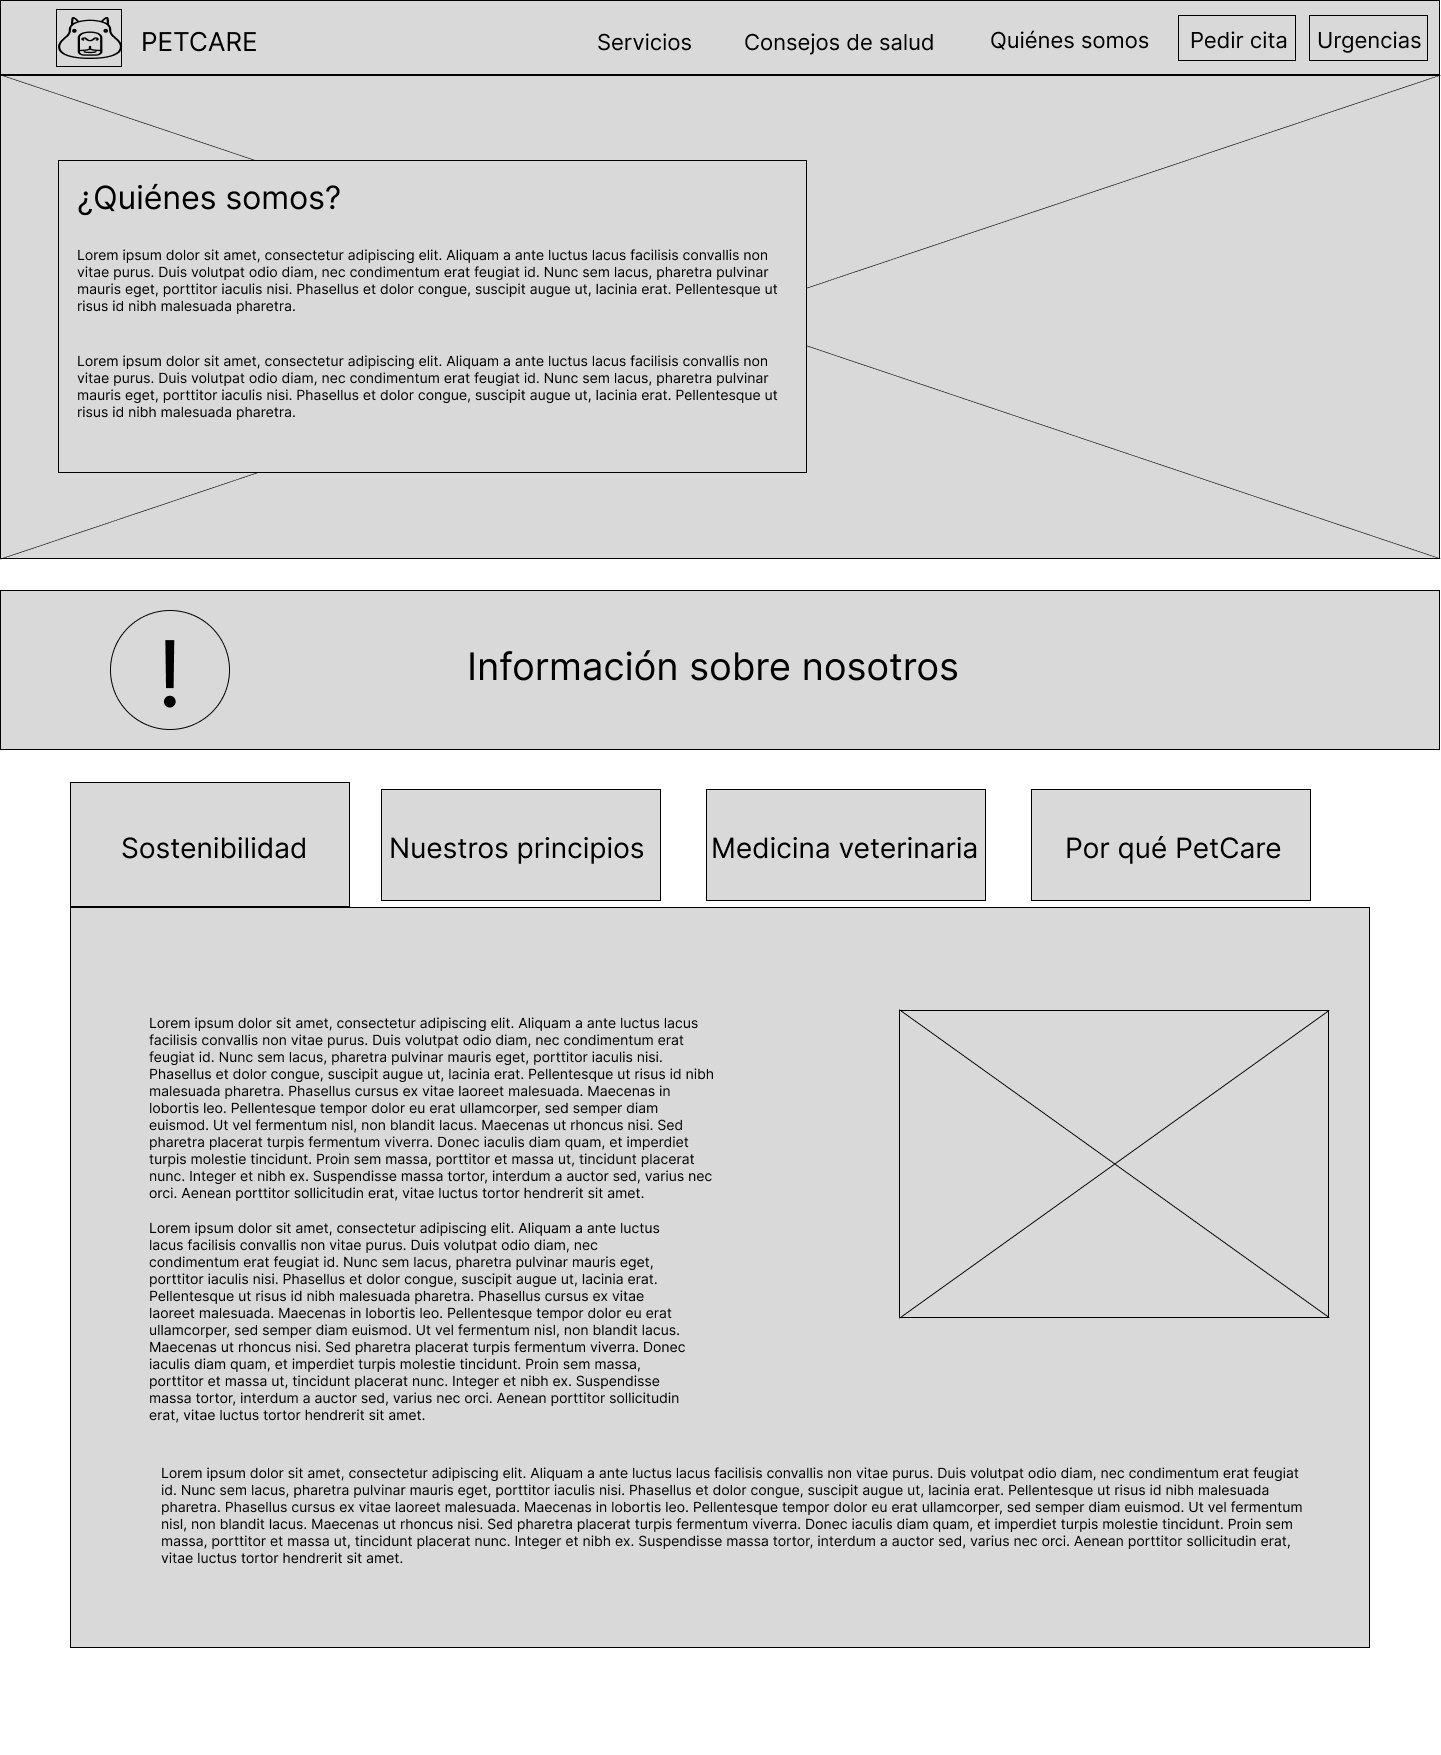
\includegraphics[width=\linewidth,height=0.95\textheight,keepaspectratio]{imgs_documento/wireframes/Wireframe_QuienesSomos.png}
\caption{Wireframe de página de información sobre la franquicia}
\end{figure}
\clearpage

\subsubsection{Consejos de salud}
\begin{figure}[H]
\centering
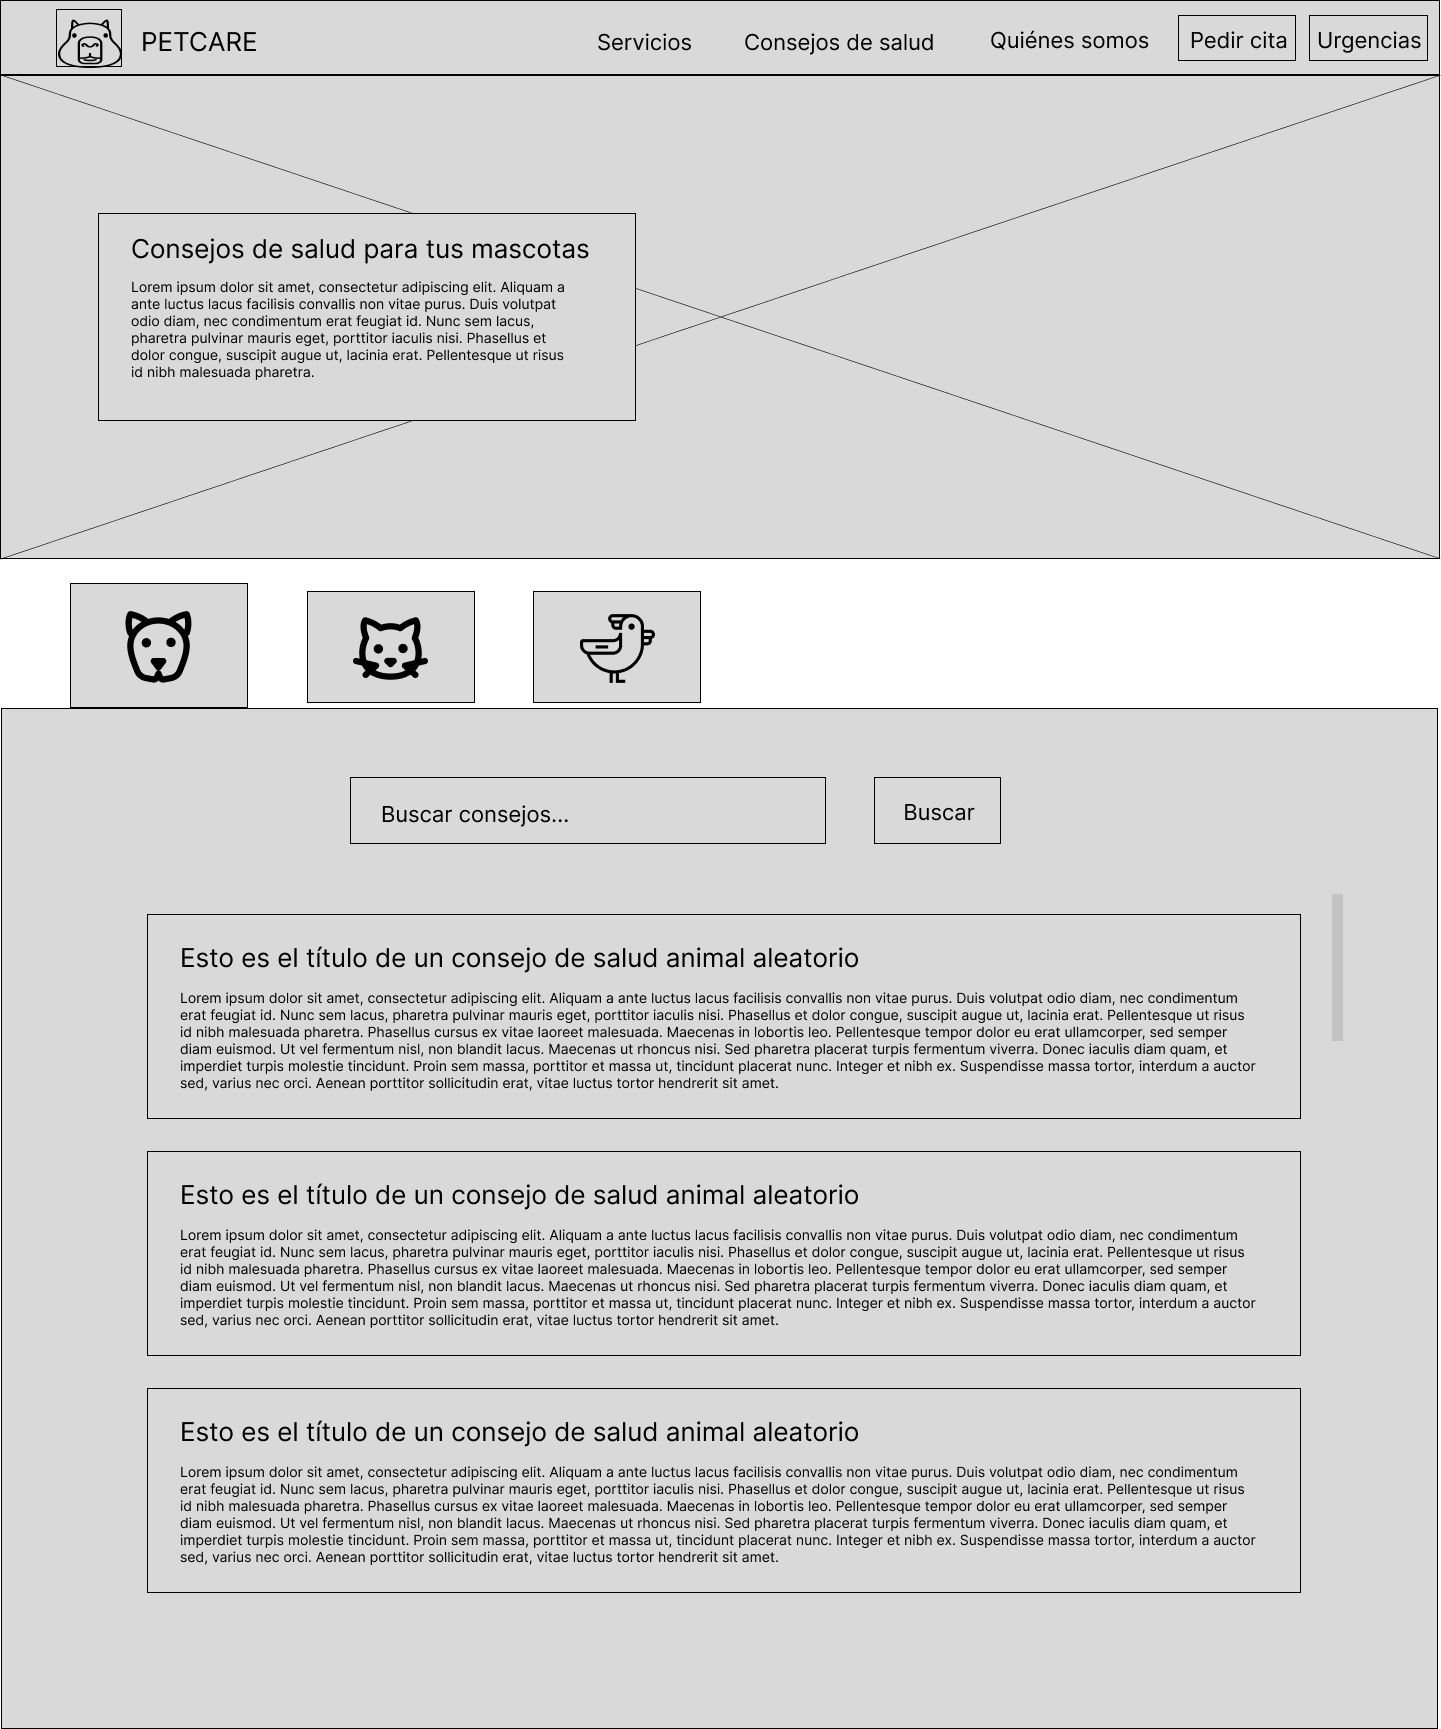
\includegraphics[width=\linewidth,height=0.95\textheight,keepaspectratio]{imgs_documento/wireframes/Wireframe_Consejos-de-salud.png}
\caption{Wireframe de la página de consejos de salud para mascotas}
\end{figure}
\clearpage

\subsubsection{Consejo específico}
\begin{figure}[H]
\centering
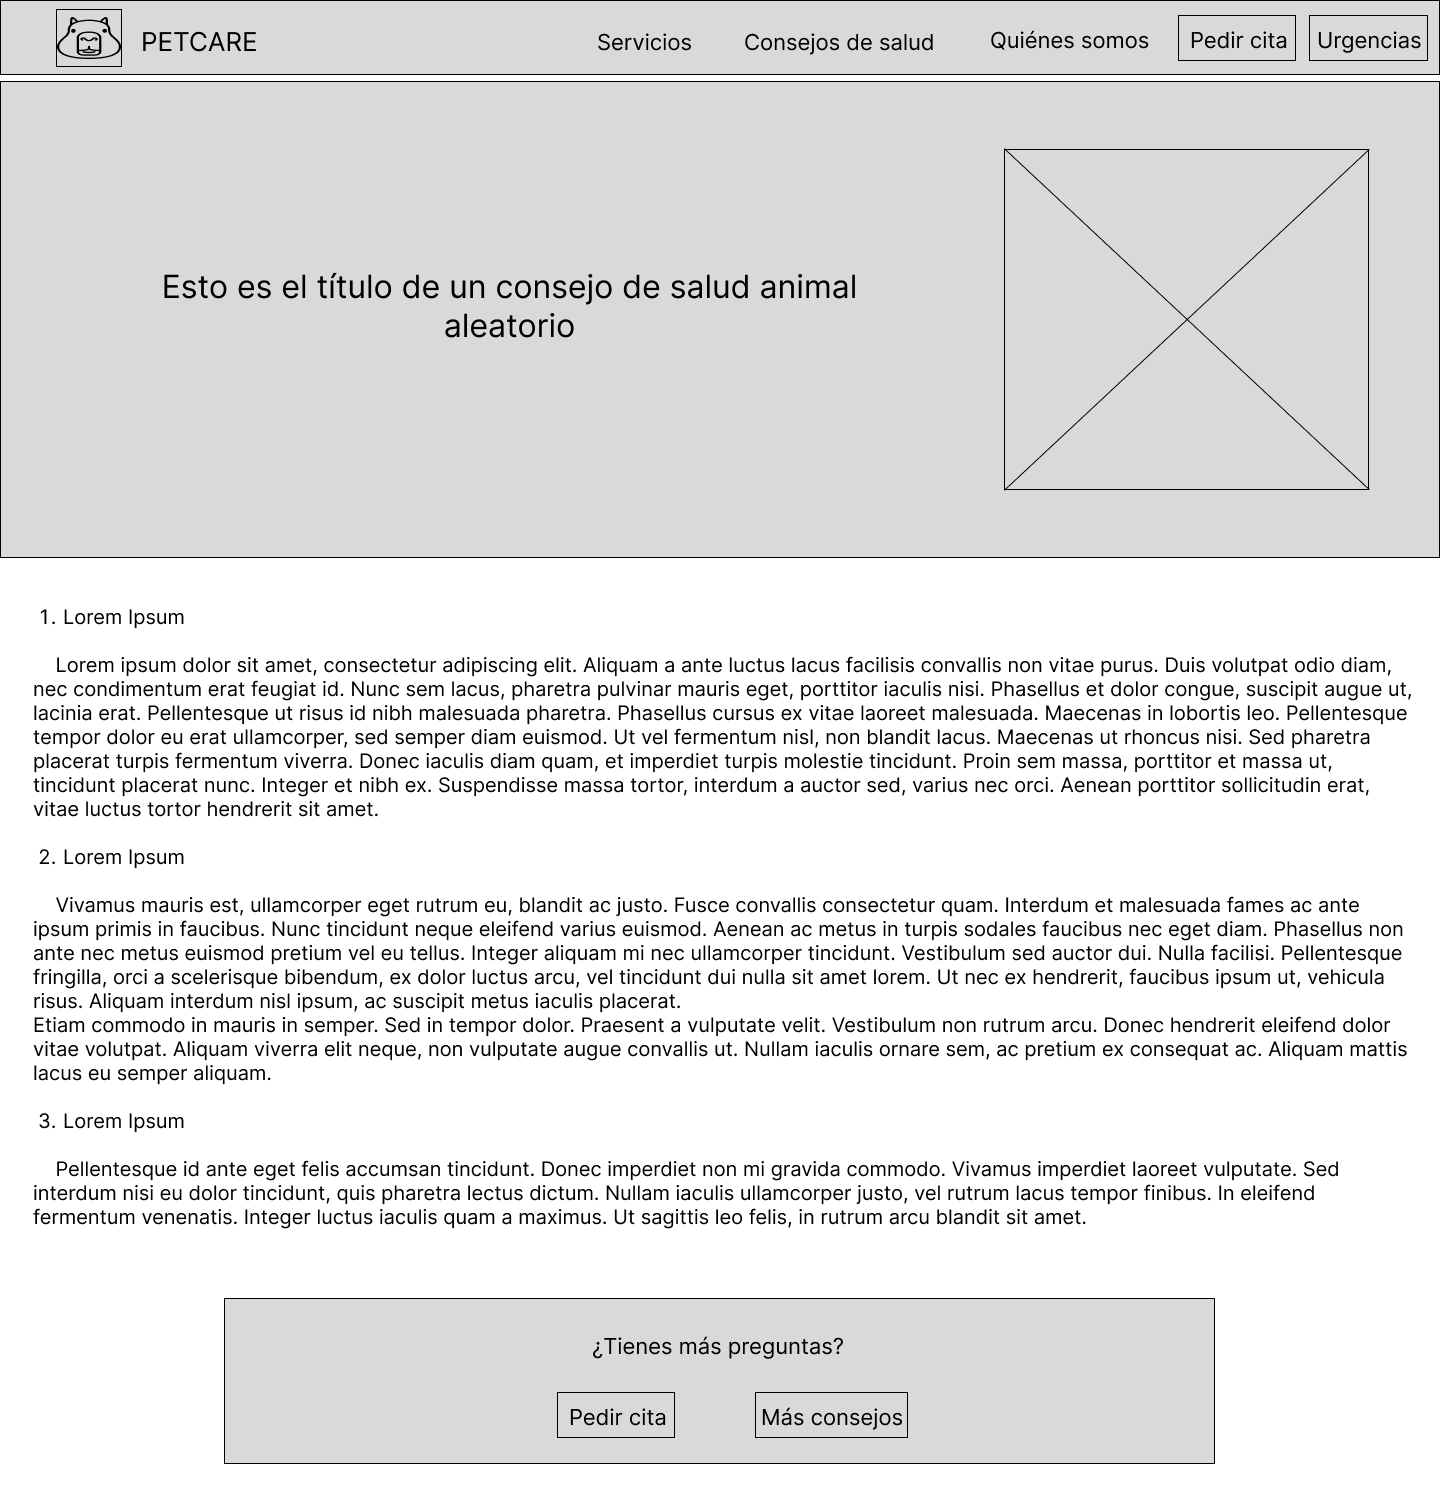
\includegraphics[width=\linewidth,height=0.95\textheight,keepaspectratio]{imgs_documento/wireframes/Wireframe_ConsejoSalud.png}
\caption{Wireframe de la página de un consejo de salud específico}
\end{figure}
\clearpage

\subsubsection{Solicitud de cita}
\begin{figure}[H]
\centering
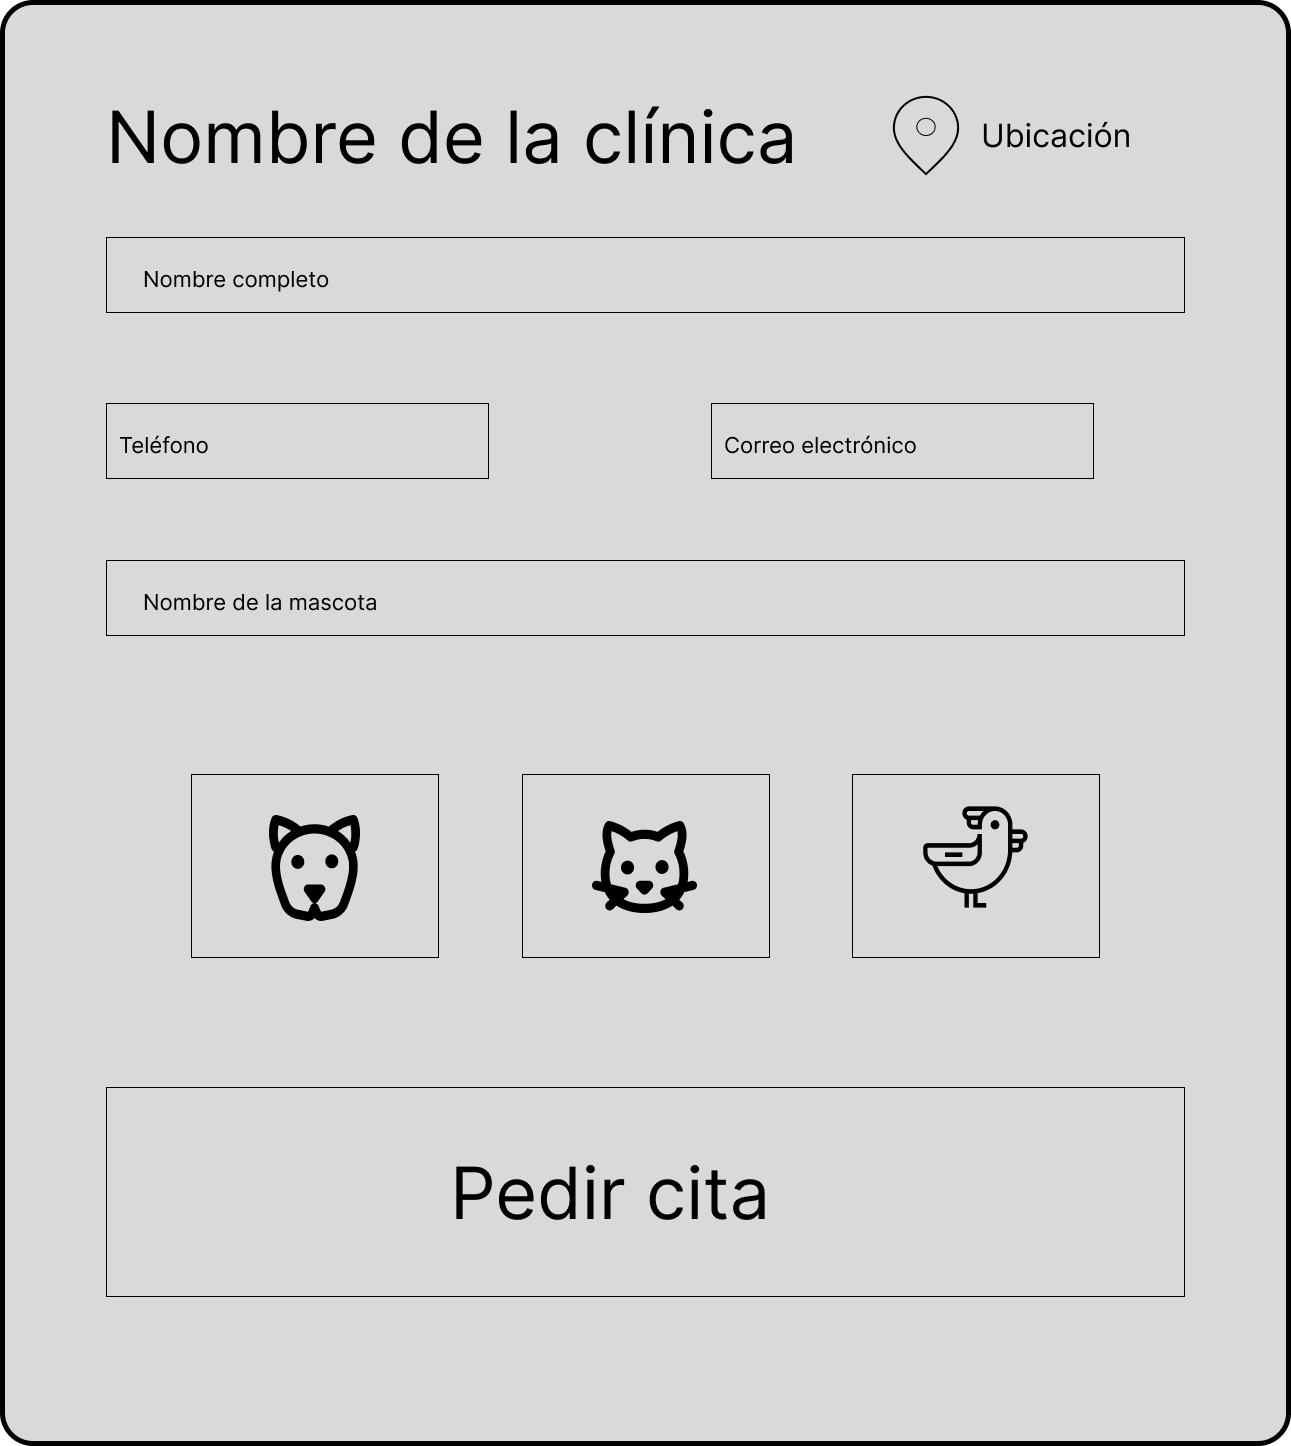
\includegraphics[width=\linewidth,height=0.95\textheight,keepaspectratio]{imgs_documento/wireframes/Wireframe_ventanaModalCita.png}
\caption{Wireframe del formulario para “Pedir cita”}
\end{figure}

\subsection{Mockups}

\subsubsection{Página principal}
\begin{figure}[H]
\centering
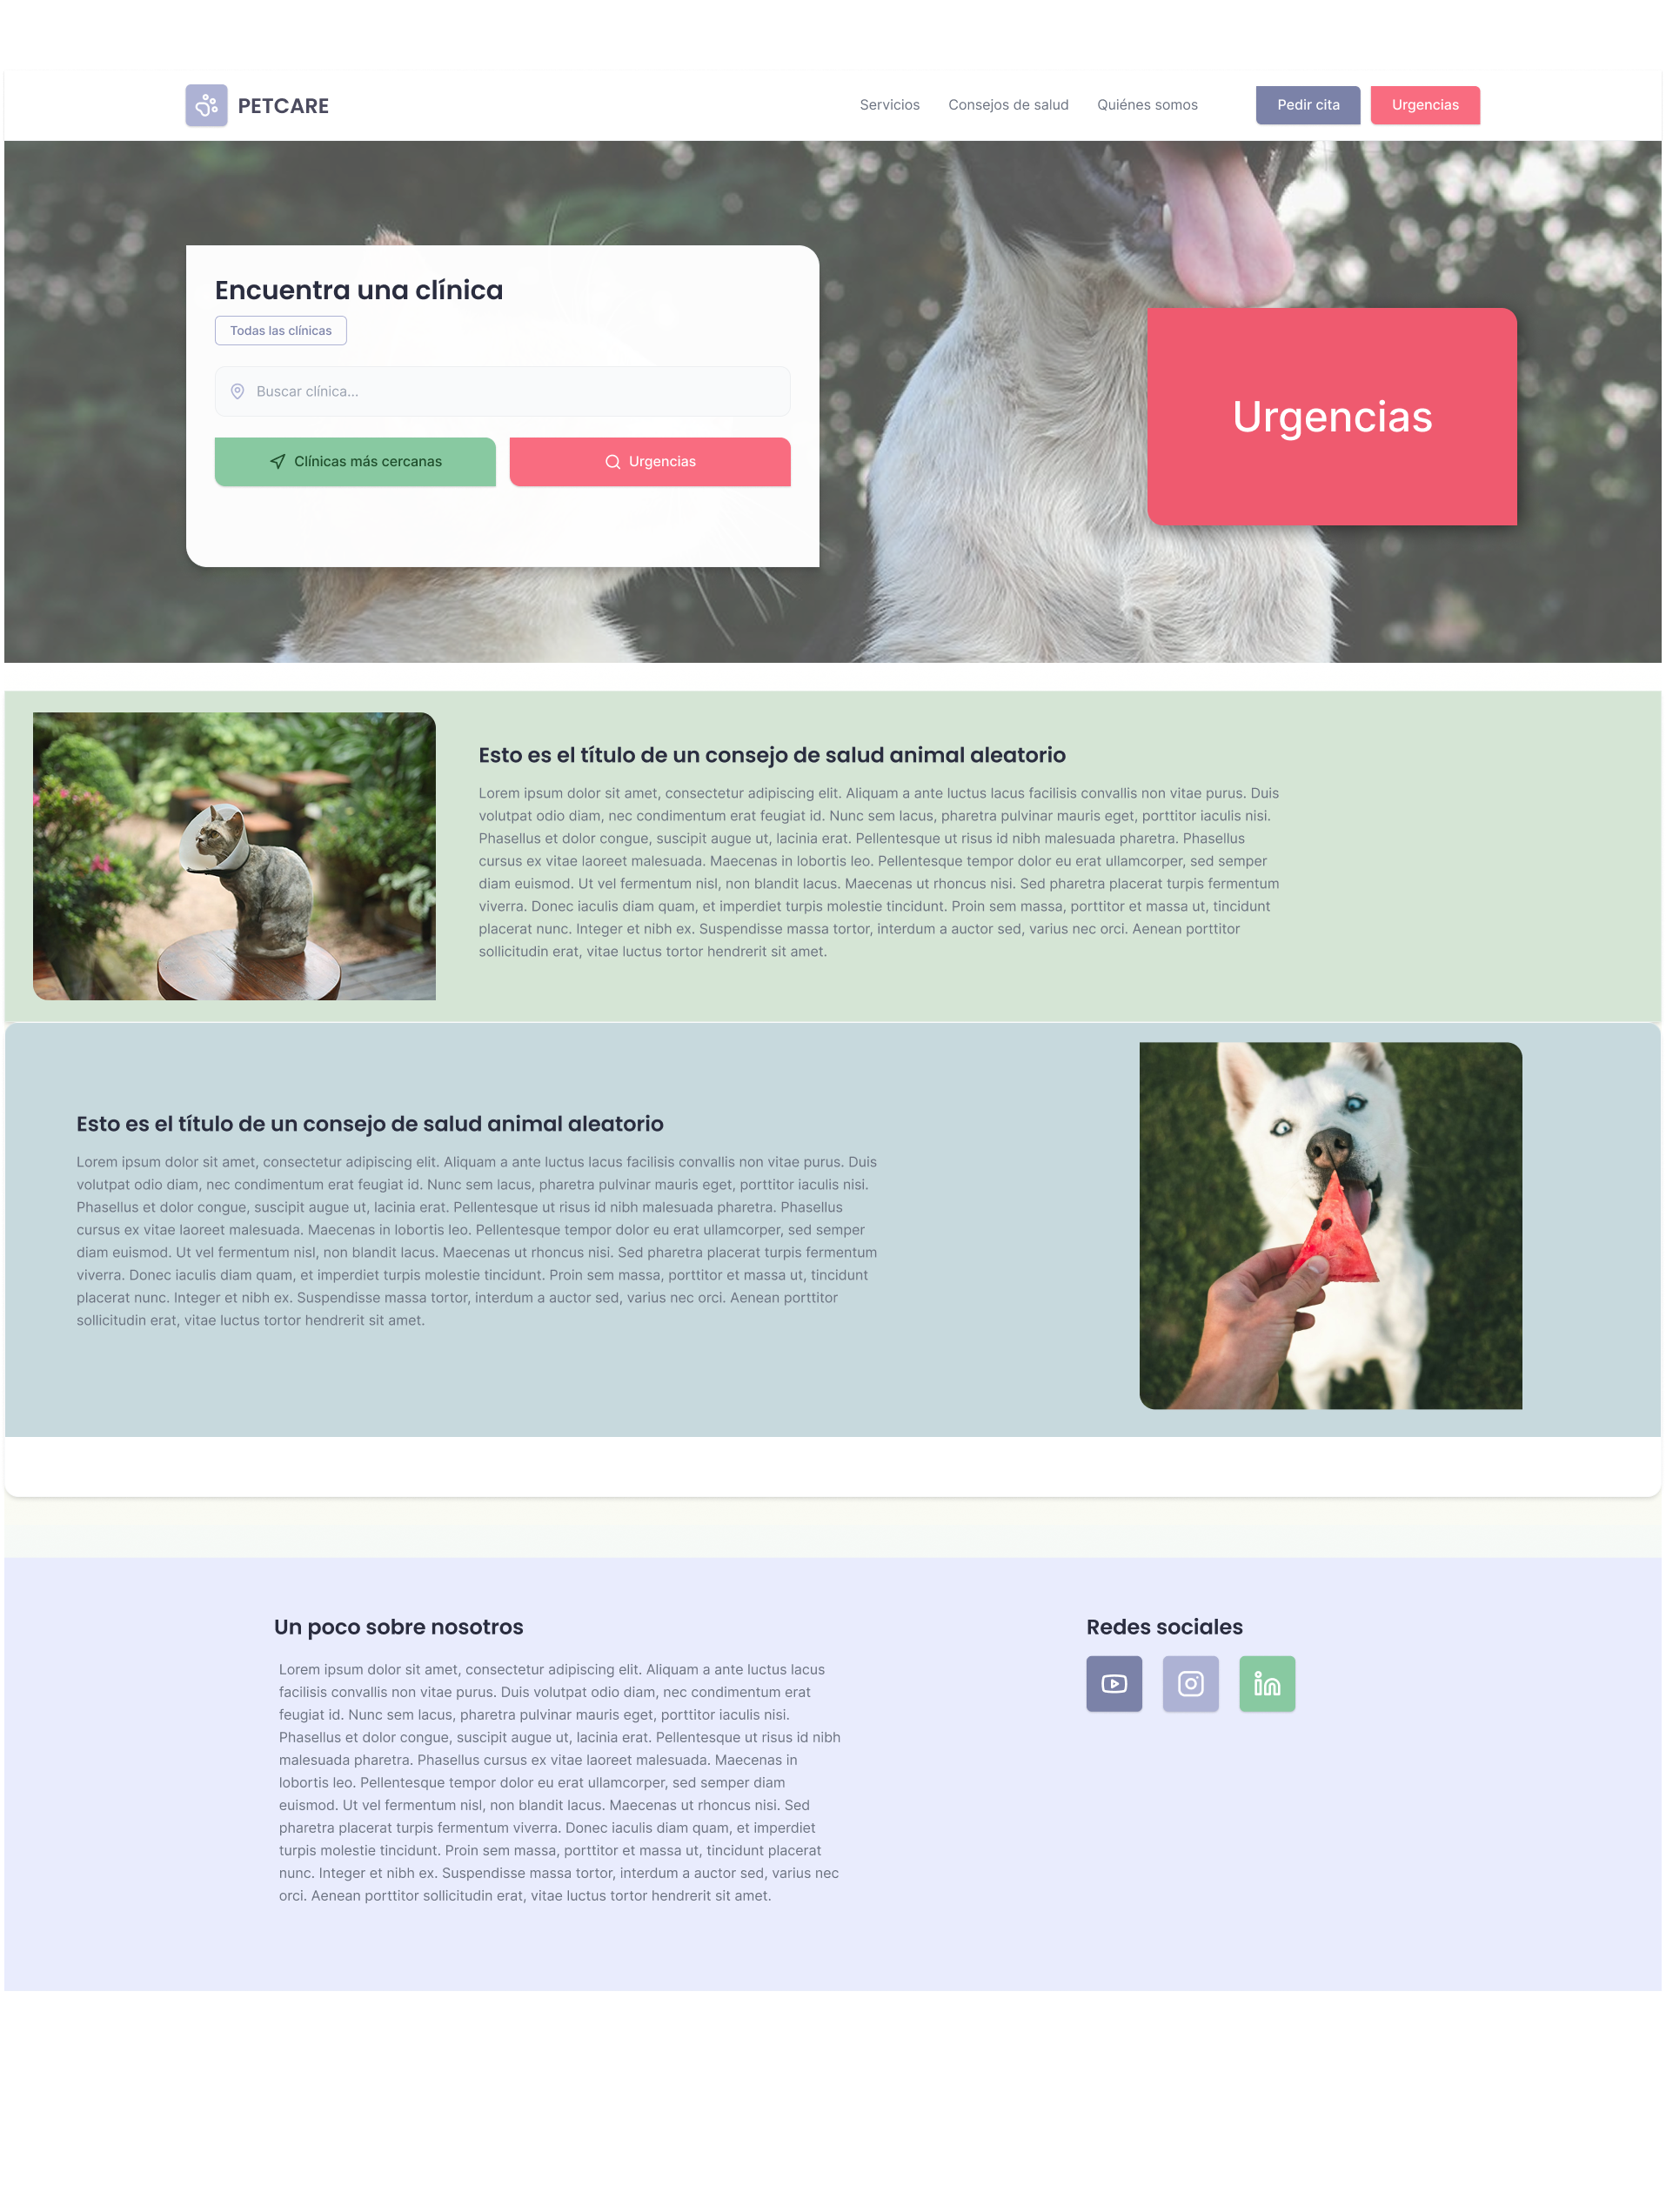
\includegraphics[width=\linewidth,height=0.95\textheight,keepaspectratio]{imgs_documento/mockups/home.png}
\caption{Mockup de página principal}
\end{figure}
\clearpage

\subsubsection{Clínicas}
\begin{figure}[H]
\centering

\includegraphics[width=\linewidth,height=0.95\textheight,keepaspectratio]{imgs_documento/mockups/clinicas.png}
\caption{Mockup de página de clínicas}
\end{figure}
\clearpage

\subsubsection{Urgencias}
\begin{figure}[H]
\centering

\includegraphics[width=\linewidth,height=0.95\textheight,keepaspectratio]{imgs_documento/mockups/urgencias.png}
\caption{Mockup de página de urgencias}
\end{figure}
\clearpage

\subsubsection{Servicios y tratamientos}
\begin{figure}[H]
\centering

\includegraphics[width=\linewidth,height=0.95\textheight,keepaspectratio]{imgs_documento/mockups/servicios.png}
\caption{Mockup de página de servicios y tratamientos}
\end{figure}
\clearpage

\subsubsection{Consejos de salud}
\begin{figure}[H]
\centering

\includegraphics[width=\linewidth,height=0.95\textheight,keepaspectratio]{imgs_documento/mockups/consejos.png}
\caption{Mockup de la página de consejos de salud para mascotas}
\end{figure}
\clearpage

\subsubsection{Sobre nosotros}
\begin{figure}[H]
\centering
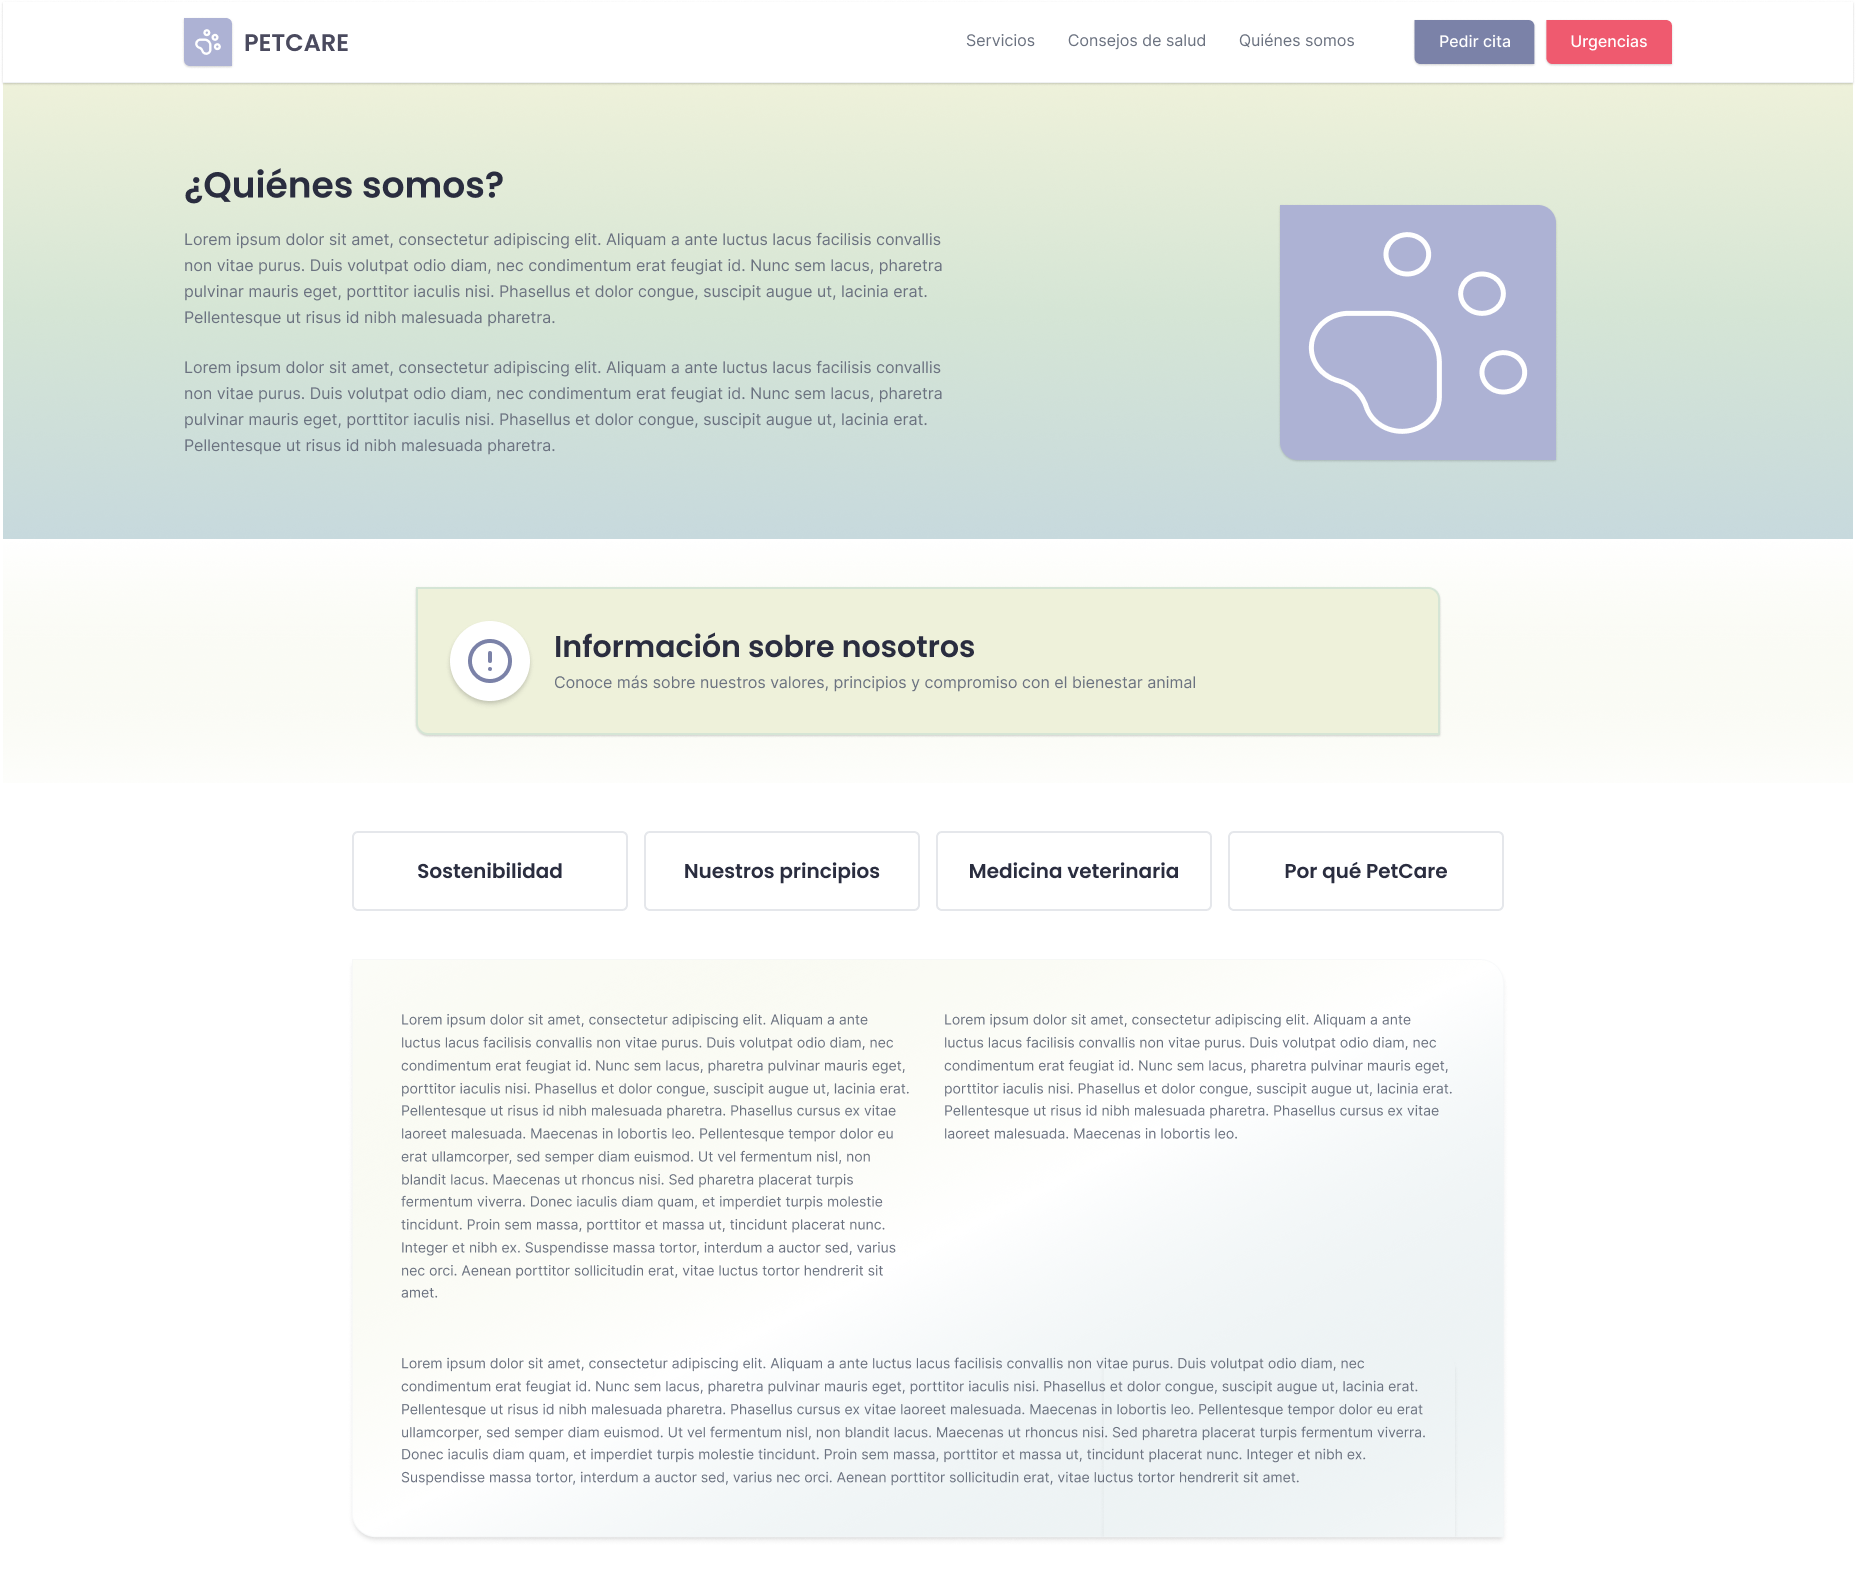
\includegraphics[width=\linewidth,height=0.95\textheight,keepaspectratio]{imgs_documento/mockups/quienes-somos.png}
\caption{Mockup de página de información sobre la franquicia}
\end{figure}
\clearpage

\subsubsection{Servicio específico}
\begin{figure}[H]
\centering

\includegraphics[width=\linewidth,height=0.95\textheight,keepaspectratio]{imgs_documento/mockups/servicio-especifico.png}
\caption{Mockup de la página de un servicio específico}
\end{figure}
\clearpage

\subsubsection{Solicitud de cita}
\begin{figure}[H]
\centering
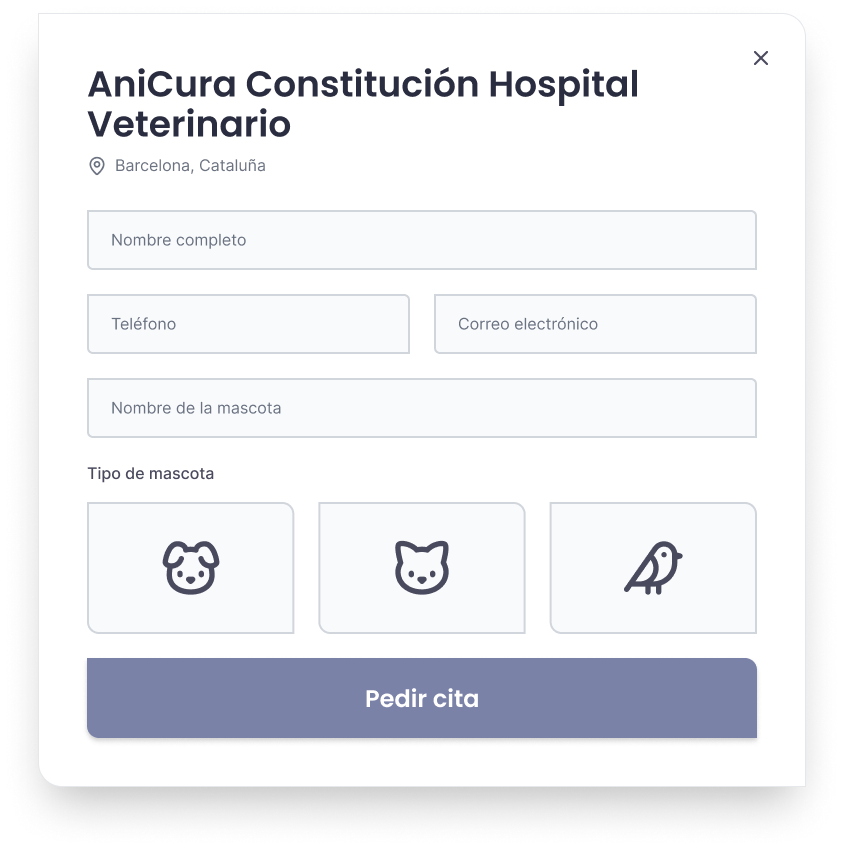
\includegraphics[width=\linewidth,height=0.95\textheight,keepaspectratio]{imgs_documento/mockups/pedir.cita.png}
\caption{Mockup del formulario para pedir cita}
\end{figure}

\section{Estructura de ficheros}

\begin{figure}[H]
\centering
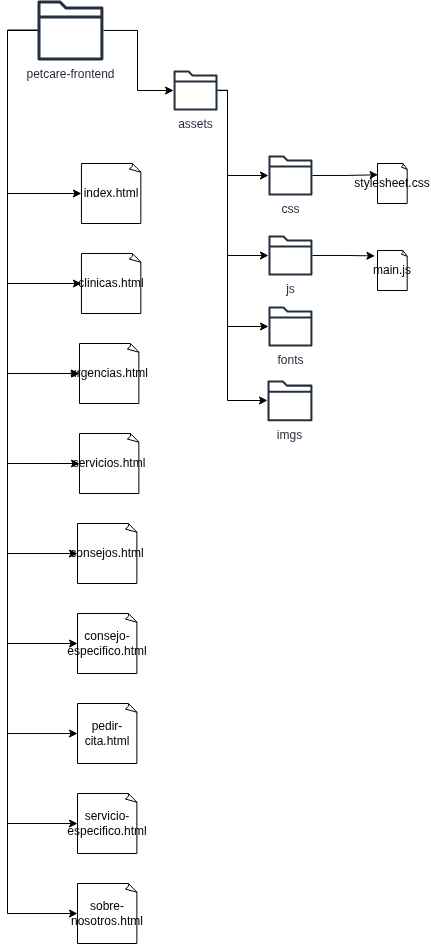
\includegraphics[width=\linewidth,height=0.95\textheight,keepaspectratio]{imgs_documento/estructuraDeFicheros.png}
\caption{Estructura de ficheros}
\end{figure}


\section{Mapas de etiquetas HTML}

\subsection{Página principal}
\begin{figure}[H]
\centering

\includegraphics[width=\linewidth,height=0.95\textheight,keepaspectratio]{mapasDeEtiquetas/index-boxmodel.png}
\caption{Mapa de etiquetas modelado en cajas de la página principal}
\end{figure}

\subsection{Clínicas}
\begin{figure}[H]
\centering

\includegraphics[width=\linewidth,height=0.95\textheight,keepaspectratio]{mapasDeEtiquetas/clinicas-boxmodel.png}
\caption{Mapa de etiquetas modelado en cajas de la página de clínicas}
\end{figure}

\subsection{Urgencias}
\begin{figure}[H]
\centering

\includegraphics[width=\linewidth,height=0.95\textheight,keepaspectratio]{mapasDeEtiquetas/urgencias-boxmodel.png}
\caption{Mapa de etiquetas modelado en cajas de la página de urgencias}
\end{figure}

\subsection{Servicios y tratamientos}
\begin{figure}[H]
\centering

\includegraphics[width=\linewidth,height=0.95\textheight,keepaspectratio]{mapasDeEtiquetas/servicios-boxmodel.png}
\caption{Mapa de etiquetas modelado en cajas de la página de servicios y tratamientos}
\end{figure}

\subsection{Servicio específico}
\begin{figure}[H]
\centering

\includegraphics[width=\linewidth,height=0.95\textheight,keepaspectratio]{mapasDeEtiquetas/servicio-especifico-boxmodel.png}
\caption{Mapa de etiquetas modelado en cajas de la página de un servicio específico}
\end{figure}

\subsection{Sobre nosotros}
\begin{figure}[H]
\centering

\includegraphics[width=\linewidth,height=0.95\textheight,keepaspectratio]{mapasDeEtiquetas/sobre-nosotros-boxmodel.png}
\caption{Mapa de etiquetas modelado en cajas de la página de información sobre la franquicia}
\end{figure}

\subsection{Consejos de salud}
\begin{figure}[H]
\centering

\includegraphics[width=\linewidth,height=0.95\textheight,keepaspectratio]{mapasDeEtiquetas/consejos-boxmodel.png}
\caption{Mapa de etiquetas modelado en cajas de la página de consejos de salud}
\end{figure}

\subsection{Consejo específico}
\begin{figure}[H]
\centering

\includegraphics[width=\linewidth,height=0.95\textheight,keepaspectratio]{mapasDeEtiquetas/consejo-especifico-boxmodel.png}
\caption{Mapa de etiquetas modelado en cajas de la página de un consejo específico}
\end{figure}

\subsection{Solicitud de cita}
\begin{figure}[H]
\centering

\includegraphics[width=\linewidth,height=0.95\textheight,keepaspectratio]{mapasDeEtiquetas/pedir-cita-boxmodel.png}
\caption{Mapa de etiquetas modelado en cajas del formulario para pedir cita}
\end{figure}

% =============================================================================
\section{Práctica 3: Responsividad}
% =============================================================================

En esta práctica se ha dotado al sitio web de un diseño responsivo aplicando cinco técnicas distintas, cada una en una página diferente, tal y como indica el enunciado. En todos los casos se sigue una filosofía \textit{Mobile First}, priorizando la visualización en dispositivos pequeños y escalando hacia pantallas mayores mediante \textit{Media Queries}.

% ─────────────────────────────────────────────────────────────────────────────
\subsection{Flexible Grids con \texttt{float} --- Clínicas}
% ─────────────────────────────────────────────────────────────────────────────

En la sección de clínicas, hemos implementado el patrón de diseño \textit{Flexible Grids} apoyado en el uso de elementos flotantes (\texttt{float}). Esta decisión se enmarca dentro de una filosofía \textit{Mobile First}, priorizando el rendimiento y la correcta visualización en dispositivos móviles por defecto, para posteriormente escalar el diseño hacia pantallas de mayor tamaño.

Por defecto (para pantallas pequeñas), las tarjetas de las clínicas se comportan como elementos de bloque estándar, ocupando el 100\% del ancho disponible y apilándose verticalmente en una única columna.

Sin embargo, cuando el ancho de la ventana supera nuestro punto de quiebre de 992 píxeles (dispositivos de escritorio), entra en acción nuestra \textit{Media Query}. En este punto, el contenedor altera el comportamiento de sus elementos hijos (\texttt{<li>}) de la siguiente manera:

\begin{itemize}
\item \textbf{Uso de unidades relativas:} Se abandona el ancho del 100\% y se asigna a cada tarjeta un \texttt{width} del 47\%, un tamaño relativo que permite que el diseño fluya y se estire proporcionalmente al tamaño del contenedor padre.
\item \textbf{Flujos opuestos:} Utilizamos el pseudo-selector \texttt{:nth-child} para distinguir entre elementos pares e impares. Los elementos impares flotan a la izquierda (\texttt{float: left}) con un margen derecho del 6\% (completando así el 100\% del ancho disponible: 47\% + 6\% + 47\%). Los elementos pares flotan a la derecha (\texttt{float: right}).
\item \textbf{Limpieza de floats:} Para evitar que las tarjetas de diferentes filas colisionen o se solapen debido a diferencias de altura, aplicamos la propiedad \texttt{clear: both} a los elementos impares, forzando un salto de línea limpio para cada nueva fila del \textit{grid}.
\end{itemize}

A continuación, se detalla el código CSS utilizado para lograr este comportamiento:

\begin{lstlisting}[language=CSS, caption=Implementación de Flexible Grids para las tarjetas de clínicas]
.contenedor-tarjetas {
	list-style: none;
	width: 100%;
	overflow: hidden; /* Limpia el desbordamiento de los floats hijos */
	margin: auto;
}
/* Comportamiento por defecto (Mobile First) */
.contenedor-tarjetas li {
	width: 100%;
	float: none;
	margin: 20px auto;
}
/* Escalado a pantallas grandes (Desktop) */
@media screen and (min-width: 992px) {
	.contenedor-tarjetas {
		margin-top: 2rem;
		margin-bottom: 5rem;
		padding: 2rem;
	}
	.contenedor-tarjetas li {
		width: 47%;
		margin-bottom: 2rem;
	}
	/* Tarjetas de la izquierda */
	.contenedor-tarjetas li:nth-child(odd) {
		float: left;
		margin-right: 6%;
		clear: both; /* Fuerza el inicio de una nueva fila */
	}
	/* Tarjetas de la derecha */
	.contenedor-tarjetas li:nth-child(even) {
		float: right;
		margin-right: 0;
	}
}
\end{lstlisting}

Las siguientes capturas muestran el comportamiento responsivo de la página de clínicas en escritorio y en móvil:

\begin{figure}[H]
\centering
\rotatebox{90}{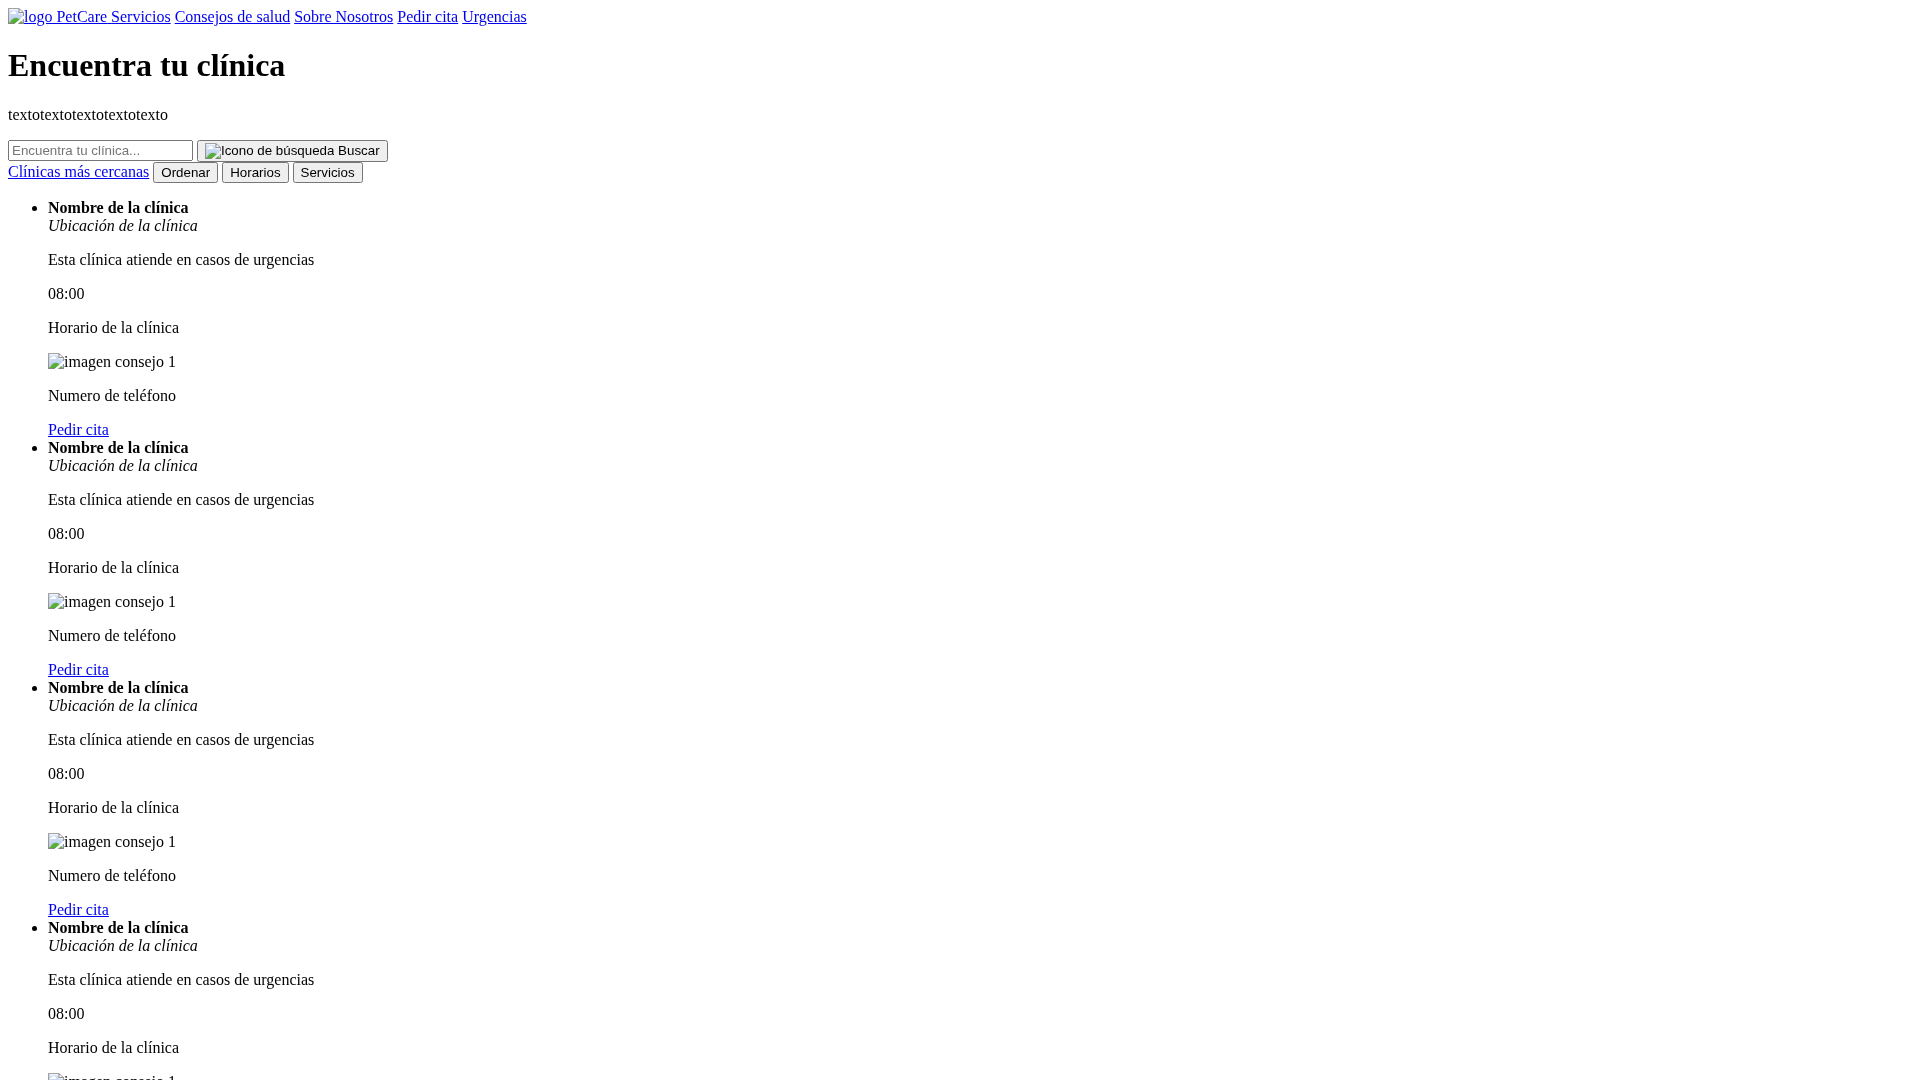
\includegraphics[width=0.85\textheight,keepaspectratio]{capturas_responsivas/clinicas-desktop.png}}
\caption{Clínicas: versión escritorio}
\end{figure}

\begin{figure}[H]
\centering
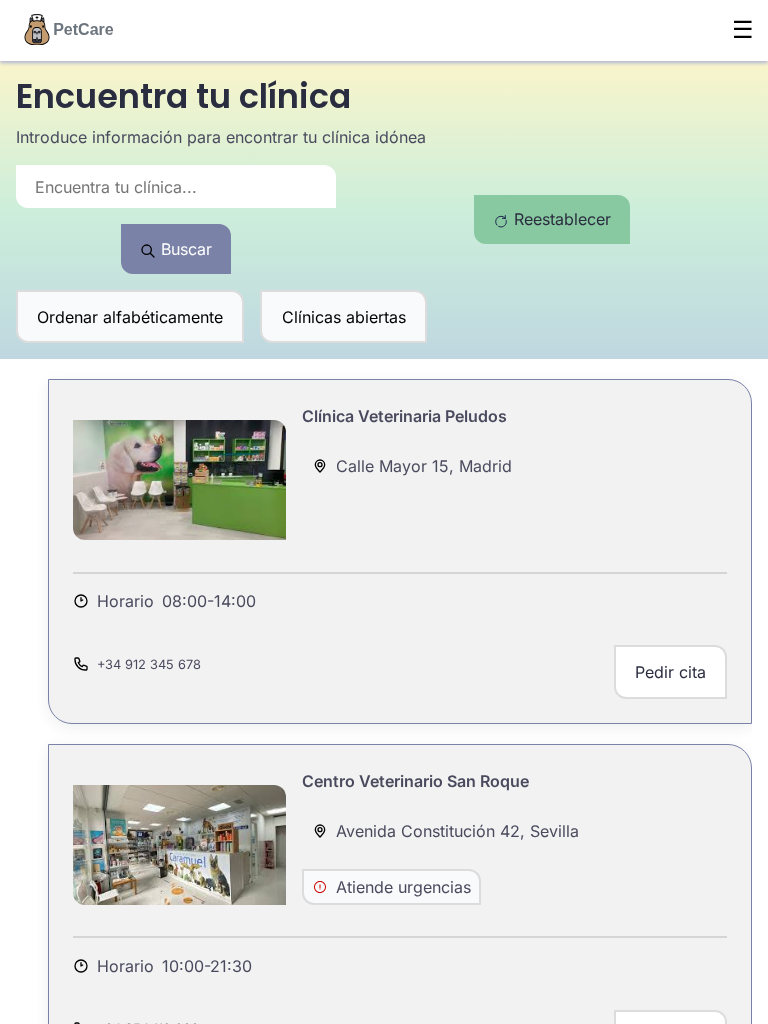
\includegraphics[width=0.65\linewidth,height=0.60\textheight,keepaspectratio]{capturas_responsivas/clinicas-tablet.png}
\caption{Clínicas: versión tablet}
\end{figure}

\begin{figure}[H]
\centering
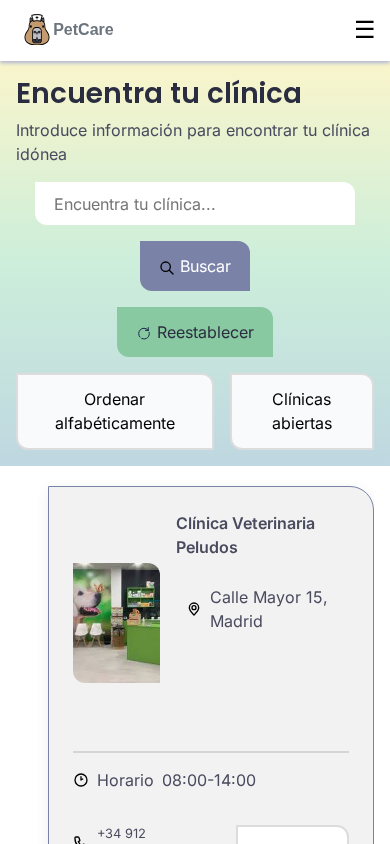
\includegraphics[width=0.38\linewidth,height=0.60\textheight,keepaspectratio]{capturas_responsivas/clinicas-mobile.png}
\caption{Clínicas: versión móvil}
\end{figure}

El mapa de etiquetas actualizado (Práctica 3) refleja los cambios introducidos respecto a la versión anterior de la página:

\begin{figure}[H]
\centering
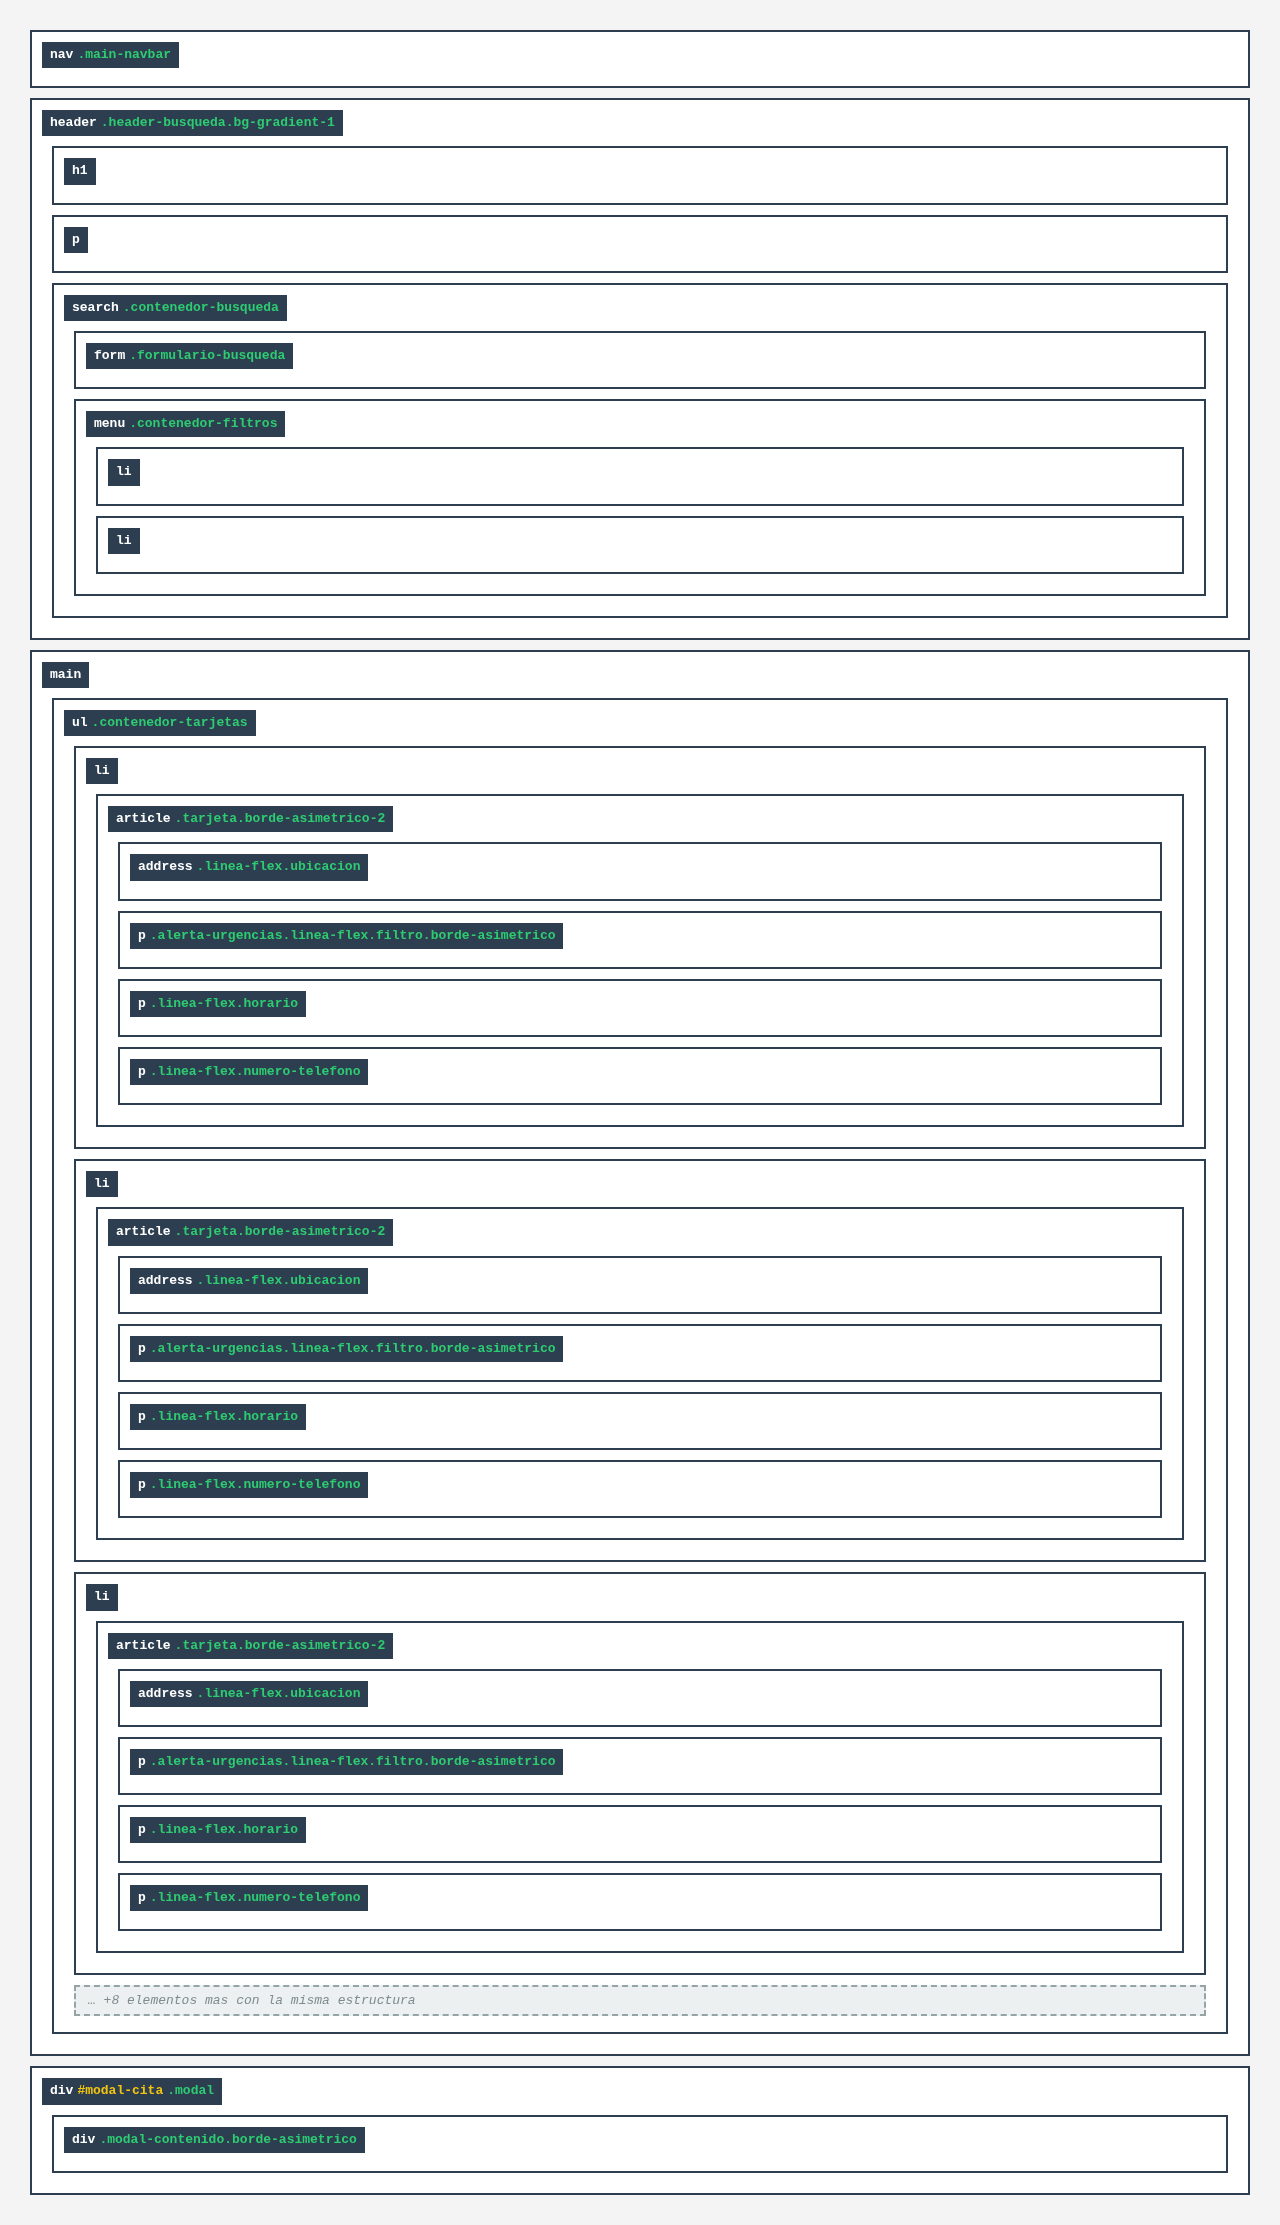
\includegraphics[width=\linewidth,height=0.85\textheight,keepaspectratio]{mapasDeEtiquetas/clinicas-boxmodel-new.png}
\caption{Mapa de etiquetas actualizado (P3) --- Clínicas}
\end{figure}

\clearpage

% ─────────────────────────────────────────────────────────────────────────────
\subsection{Diseño multicolumna --- Sobre nosotros}
% ─────────────────────────────────────────────────────────────────────────────

En la página ``Sobre nosotros'', los apartados de información extensa (Sostenibilidad, Nuestros principios, Medicina veterinaria y Por qué PetCare) requieren una estructura que facilite su lectura. Para ello, hemos utilizado las propiedades nativas del módulo \textit{Multi-column Layout} de CSS3, logrando que el texto fluya de forma automática en una o dos columnas dependiendo del dispositivo.

En monitores de escritorio, mostrar un bloque de texto que cruce la pantalla de lado a lado resulta fatigante para el ojo humano. Dividir el contenido en dos columnas (como en un periódico) acorta la longitud de las líneas y mejora la legibilidad. Sin embargo, en dispositivos móviles o tabletas pequeñas, mantener dos columnas provocaría que el texto quedara demasiado comprimido y las palabras se cortaran en exceso, por lo que la lectura debe volver a una sola columna.

Para este módulo específico, el código base establece el diseño para pantallas grandes y utilizamos una \textit{Media Query} con \texttt{max-width} para adaptar el contenido cuando la pantalla se reduce.

\begin{itemize}
\item \textbf{Diseño base (Pantallas grandes):} Asignamos al contenedor la propiedad \texttt{column-count: 2}, que le indica al navegador que divida el texto en dos columnas equitativas de forma automática. Para que el texto no se vea demasiado compacto, utilizamos \texttt{column-gap: 2rem} para establecer algo de separación entre ambas columnas. El contenedor ocupa un 75\% del ancho de la pantalla para mantener unos márgenes laterales.
\item \textbf{Punto de quiebre (Dispositivos móviles):} Cuando la pantalla es inferior a 992 píxeles, la regla \texttt{@media screen and (max-width: 992px)} se activa. Reducimos el número de columnas a una sola (\texttt{column-count: 1}). Además, ampliamos el contenedor al 95\% del ancho de la pantalla para aprovechar al máximo el espacio reducido de los teléfonos, y reducimos ligeramente el tamaño de la fuente (de \texttt{x-large} a \texttt{large}) para adaptarlo a la nueva resolución.
\end{itemize}

A continuación, se detalla el código CSS correspondiente a esta implementación:

\begin{lstlisting}[language=CSS, caption=Uso de Multi-column Layout para la adaptación de textos largos]
/* Diseño base para pantallas grandes (Escritorio) */
.contenedor-multicol {
	column-width: 50%;
	column-count: 2; /* Divide el texto en dos columnas */
	column-gap: 2rem; /* Espacio de respiracion entre columnas */
	width: 75%;
	margin: auto;
	padding: 35px;
	background: linear-gradient(0deg,
	rgba(113, 212, 154, 0.15) 50%,
	rgba(145, 210, 172, 0.15) 50%,
	rgba(255, 255, 255, 0.15) 100%);
	font-size: x-large;
}
/* Adaptacion para dispositivos moviles y tabletas */
@media screen and (max-width: 992px) {
	.contenedor-multicol {
		column-width: 50%;
		column-count: 1; /* Retorna a una unica columna vertical */
		column-gap: 2rem;
		width: 95%;
		margin: auto;
		padding: 35px;
		background: linear-gradient(0deg,
		rgba(113, 212, 154, 0.15) 50%,
		rgba(145, 210, 172, 0.15) 50%,
		rgba(255, 255, 255, 0.15) 100%);
		font-size: large;
	}
}
\end{lstlisting}

\begin{figure}[H]
\centering
\rotatebox{90}{
\includegraphics[width=0.85\textheight,keepaspectratio]{capturas_responsivas/sobre-nosotros-desktop.png}}
\caption{Sobre nosotros: versión escritorio}
\end{figure}

\begin{figure}[H]
\centering
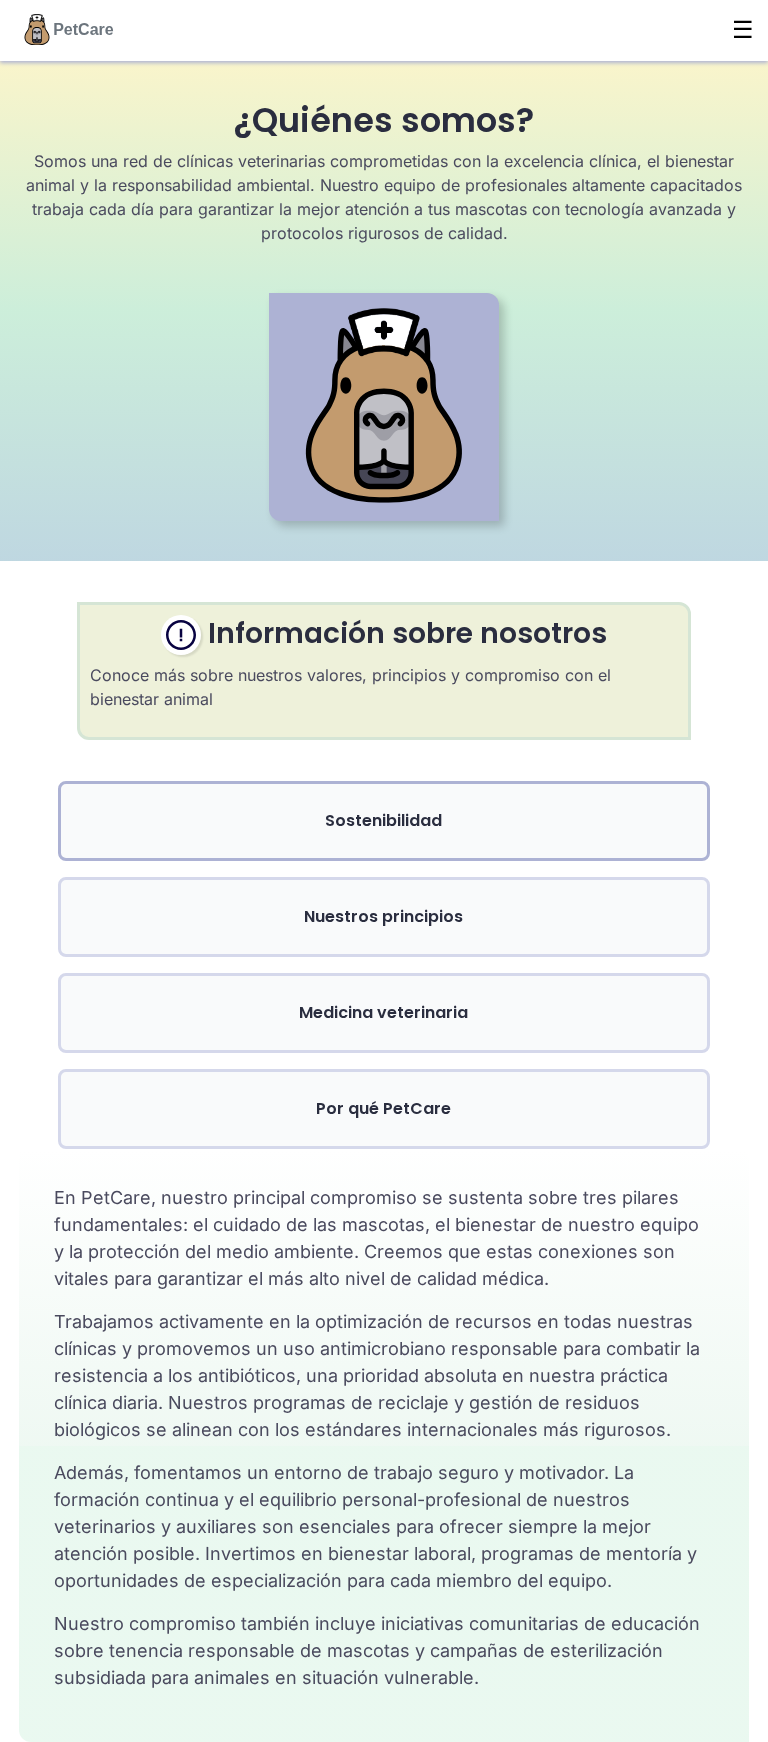
\includegraphics[width=0.65\linewidth,height=0.60\textheight,keepaspectratio]{capturas_responsivas/sobre-nosotros-tablet.png}
\caption{Sobre nosotros: versión tablet}
\end{figure}

\begin{figure}[H]
\centering
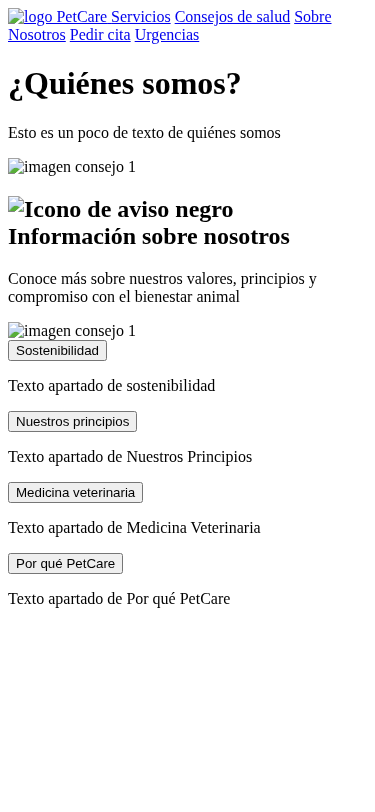
\includegraphics[width=0.38\linewidth,height=0.60\textheight,keepaspectratio]{capturas_responsivas/sobre-nosotros-mobile.png}
\caption{Sobre nosotros: versión móvil}
\end{figure}

\begin{figure}[H]
\centering
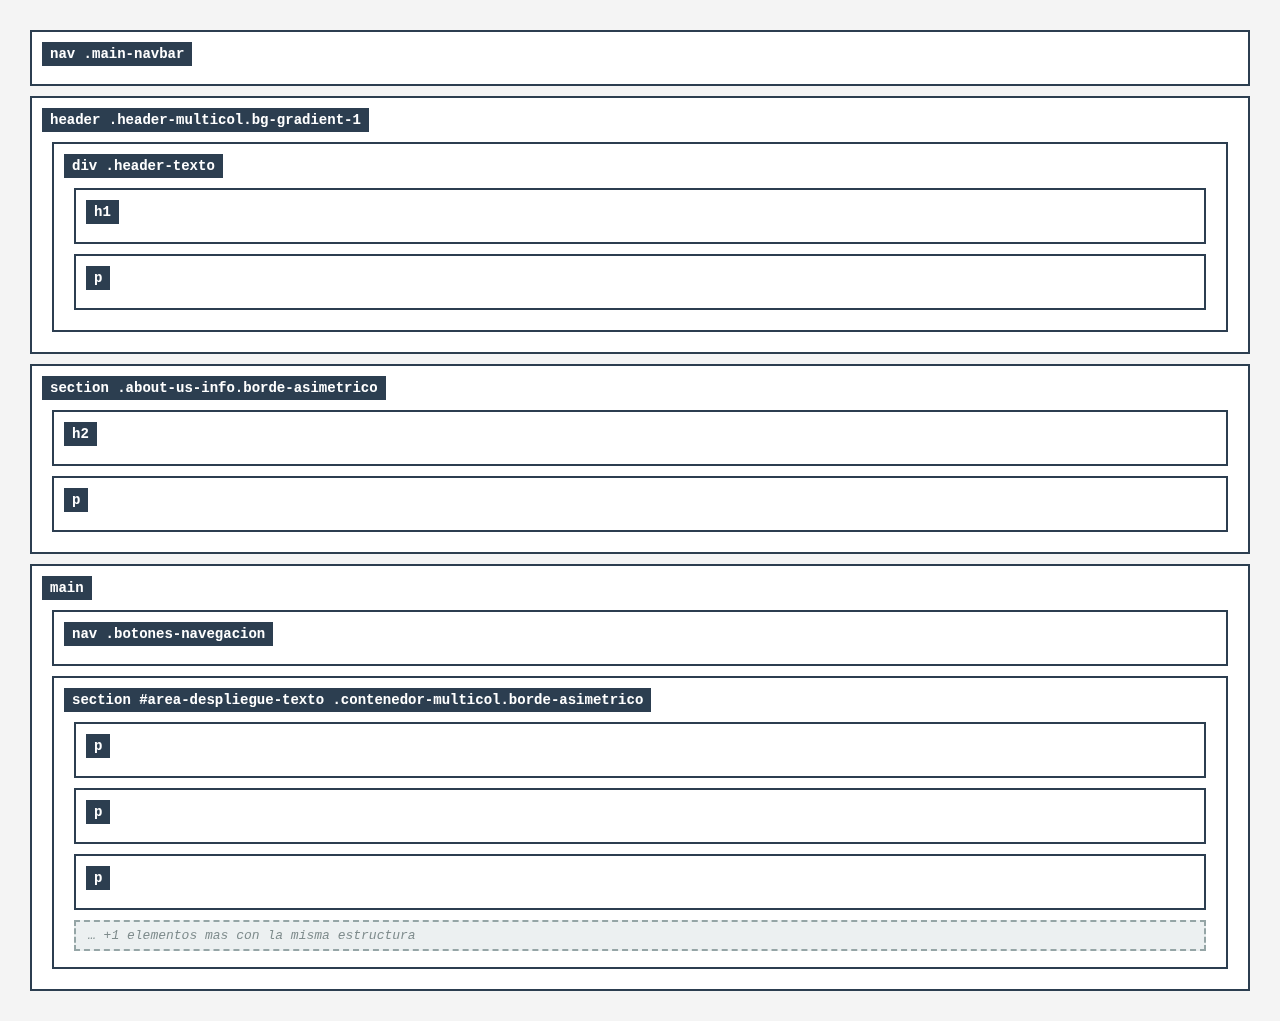
\includegraphics[width=\linewidth,height=0.85\textheight,keepaspectratio]{mapasDeEtiquetas/sobre-nosotros-boxmodel-new.png}
\caption{Mapa de etiquetas actualizado (P3) --- Sobre nosotros}
\end{figure}

\clearpage

% ─────────────────────────────────────────────────────────────────────────────
\subsection{CSS Flex Container --- Solicitud de cita}
% ─────────────────────────────────────────────────────────────────────────────

Para la página de solicitud de cita (que se abre como un iframe al hacer clic en el botón de pedir cita de la tarjeta de una clínica) hemos decidido utilizar el módulo \textit{CSS Flexbox}. A diferencia de CSS Grid, que es ideal para la estructura general de la página (pues permite la distribución bidimensional de elementos), Flexbox brilla en la alineación y distribución de elementos en una sola dimensión (filas o columnas).

Hemos aplicado Flexbox a diferentes niveles de profundidad dentro del formulario para lograr una estructura sólida e intuitiva:

\begin{itemize}
\item \textbf{Centrado global (El contenedor Body):} Convertimos el \texttt{body} del \textit{iframe} en un contenedor \texttt{flex} en dirección columna. Al sumarle \texttt{min-height: 100vh} y \texttt{justify-content: center}, logramos que todo el formulario quede perfectamente centrado verticalmente dentro de la ventana modal, independientemente del tamaño de la pantalla.
\item \textbf{Apilamiento lógico (Columnas):} Los contenedores principales como \texttt{.fieldset-propietario} y \texttt{.fieldset-mascota} utilizan \texttt{flex-direction: column}. Esto asegura que los campos de introducción de datos se apilen de arriba hacia abajo, el comportamiento natural y más accesible para rellenar un formulario.
\item \textbf{Agrupaciones horizontales (Filas):} Para optimizar el espacio, agrupamos elementos estrechos y relacionados entre sí usando \texttt{flex-direction: row}. Esto lo vemos en \texttt{\#datos-contacto} (teléfono y email), \texttt{.opciones-especie} (botones de radio para el tipo de mascota) y \texttt{.fieldset-cita} (fecha y hora). Aplicando \texttt{justify-content: space-between}, garantizamos que estos elementos se separen uniformemente ocupando todo el ancho disponible.
\item \textbf{El botón de envío:} Al botón principal (\texttt{.boton-submit}) le asignamos un \texttt{width: 100\%}. En un contexto flexible (y asumiendo que el contenedor padre permite el \texttt{flex-wrap}), forzar un ancho del 100\% empuja al botón a ocupar su propia línea independiente al final del formulario.
\end{itemize}

A continuación, se detalla el código CSS estructural que define este comportamiento:

\begin{lstlisting}[language=CSS, caption=Uso de CSS Flexbox para la maquetación del formulario de citas]
/* Centrado vertical de todo el formulario en el modal */
body {
	display: flex;
	flex-direction: column;
	justify-content: center;
	min-height: 100vh;
	margin: 0;
}
/* Apilamiento vertical para los bloques principales */
.fieldset-propietario, .fieldset-mascota {
	display: flex;
	flex-direction: column;
	gap: 0.5rem;
}
/* Distribucion en fila para campos complementarios */
#datos-contacto {
	display: flex;
	flex-direction: row;
	width: 100%;
	gap: 0.5rem;
}
/* Distribucion con separacion equitativa para fechas y opciones */
.opciones-especie, .fieldset-cita {
	display: flex;
	flex-direction: row;
	justify-content: space-between;
	gap: 0.5rem;
}
.opciones-especie {
	padding: 1rem;
}
/* Boton de envio forzado a ocupar una linea completa */
.boton-submit {
	background-color: var(--color-cta-primary);
	color: white;
	border: none;
	padding: 1rem 0rem;
	font-size: 1.5rem;
	font-weight: bold;
	width: 100%;
}
\end{lstlisting}

\begin{figure}[H]
\centering
\rotatebox{90}{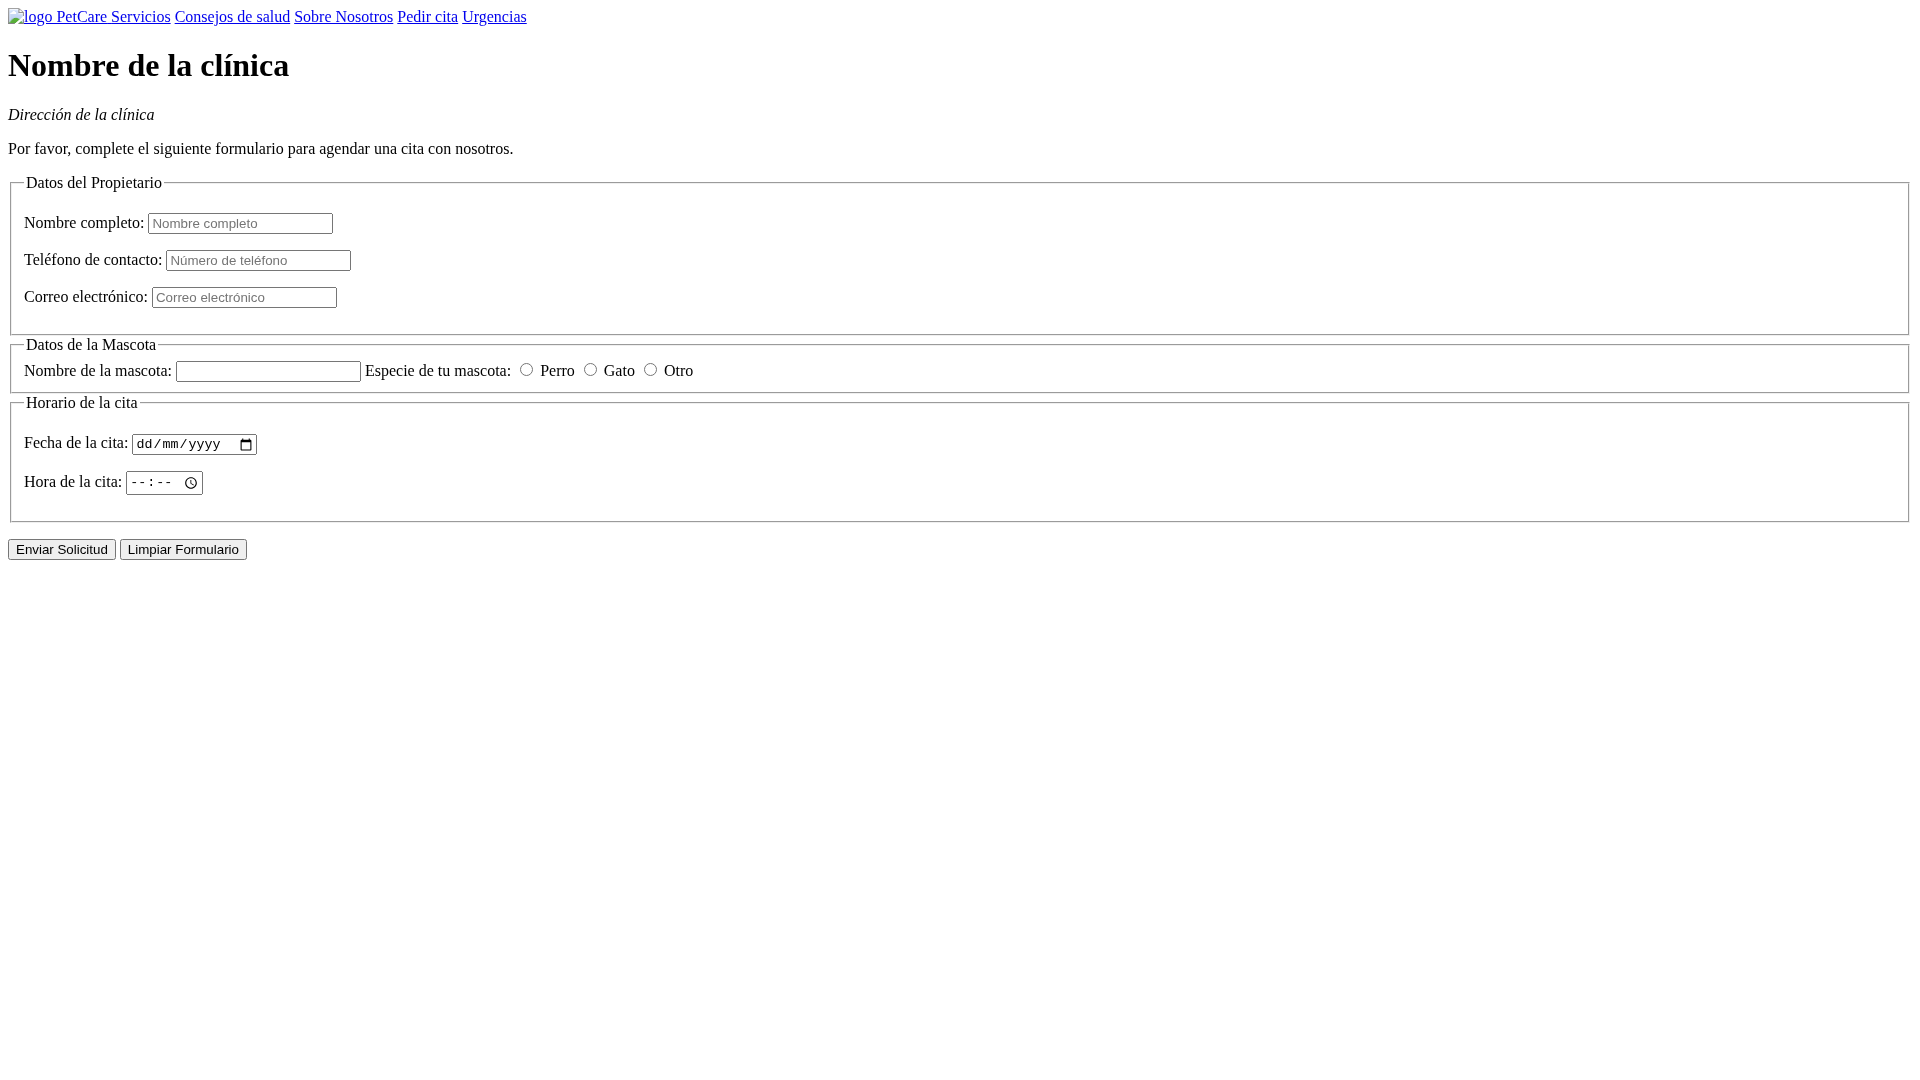
\includegraphics[width=0.85\textheight,keepaspectratio]{capturas_responsivas/pedir-cita-desktop.png}}
\caption{Solicitud de cita: versión escritorio}
\end{figure}

\begin{figure}[H]
\centering
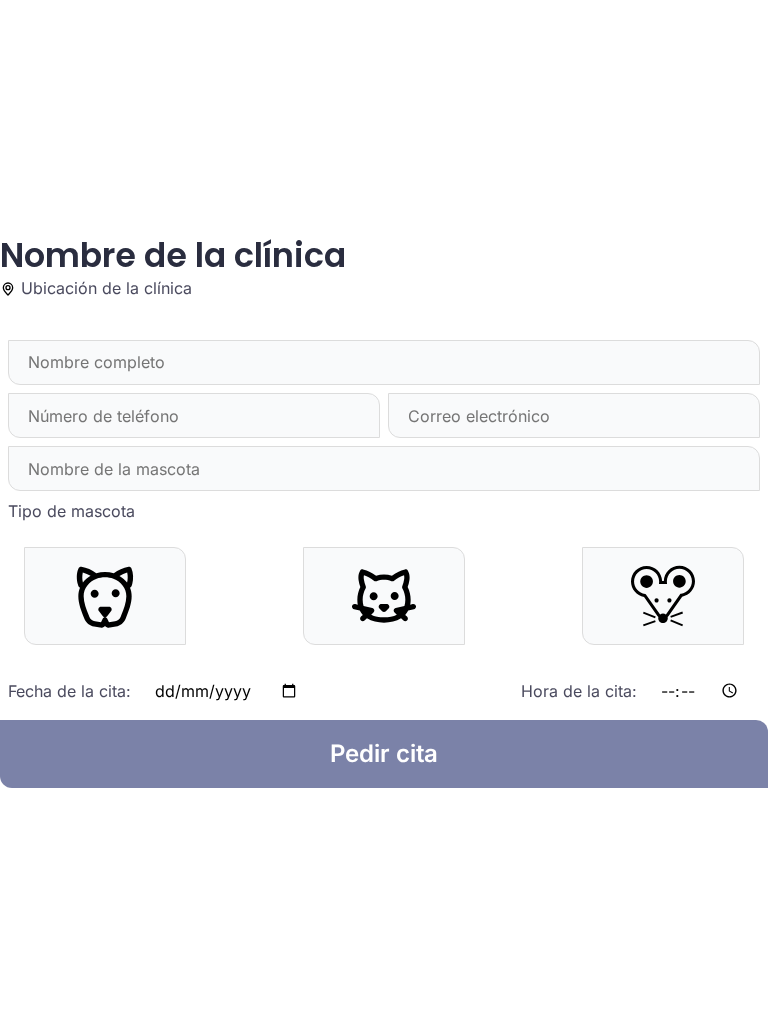
\includegraphics[width=0.65\linewidth,height=0.60\textheight,keepaspectratio]{capturas_responsivas/pedir-cita-tablet.png}
\caption{Solicitud de cita: versión tablet}
\end{figure}

\begin{figure}[H]
\centering
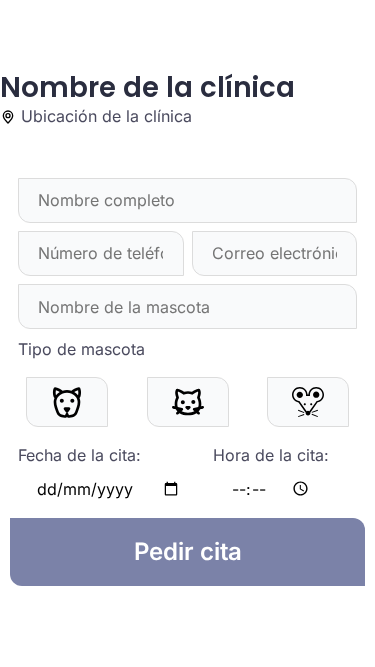
\includegraphics[width=0.38\linewidth,height=0.60\textheight,keepaspectratio]{capturas_responsivas/pedir-cita-mobile.png}
\caption{Solicitud de cita: versión móvil}
\end{figure}

\begin{figure}[H]
\centering
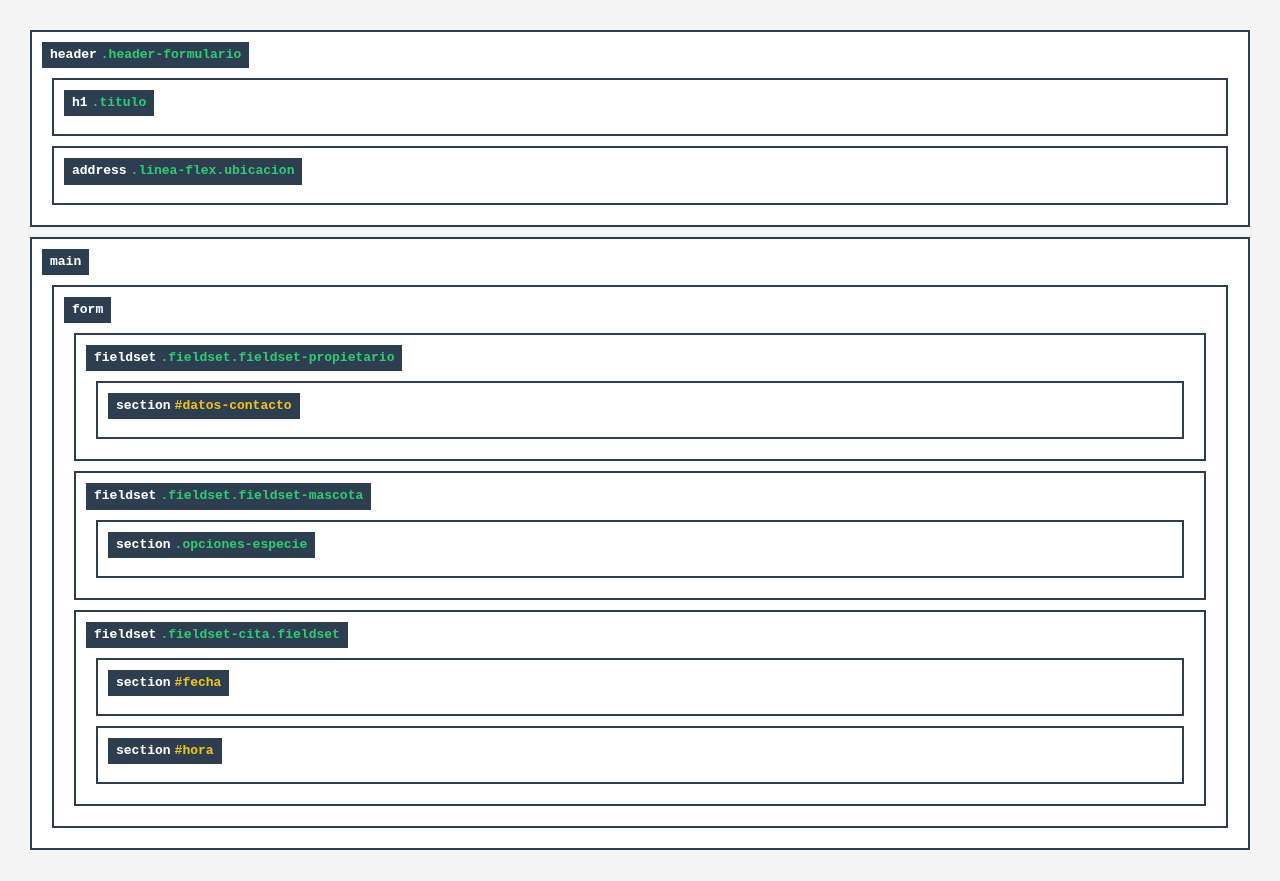
\includegraphics[width=\linewidth,height=0.85\textheight,keepaspectratio]{mapasDeEtiquetas/pedir-cita-boxmodel-new.png}
\caption{Mapa de etiquetas actualizado (P3) --- Solicitud de cita}
\end{figure}

\clearpage

% ─────────────────────────────────────────────────────────────────────────────
\subsection{CSS Grid --- Servicios}
% ─────────────────────────────────────────────────────────────────────────────

En la página de servicios, hemos optado por emplear el módulo \textit{CSS Grid Layout} para organizar la presentación de los distintos servicios ofrecidos por las clínicas. Al igual que en la estructura de las tarjetas anteriores (las tarjetas de clínicas), esta maquetación se ha desarrollado siguiendo estrictamente la metodología \textit{Mobile First}.

CSS Grid es una herramienta moderna para manejar diseños bidimensionales. A diferencia de \texttt{float} o el \textit{Multi-column Layout}, Grid nos permite definir una cuadrícula rígida pero elástica, asegurando que todas las cajas de servicios mantengan anchos uniformes y un espaciado adecuado sin necesidad de calcular márgenes porcentuales. En dispositivos móviles, una sola columna garantiza legibilidad y un tamaño adecuado para la interacción táctil. En pantallas de mayor tamaño, dividir el contenido en dos columnas evita que las cajas se estiren de forma antiestética, mejorando el escaneo visual de la información.

La implementación se articula definiendo el estado base para pantallas pequeñas y aplicando una \textit{Media Query} para el escalado en pantallas medianas y de escritorio:

\begin{itemize}
\item \textbf{Diseño base (Dispositivos móviles):} Convertimos el contenedor de la lista (\texttt{.lista-servicios}) en una cuadrícula aplicando \texttt{display: grid}. A través de la propiedad \texttt{grid-template-columns: 1fr}, ordenamos al navegador que cree una única columna que ocupe \texttt{1fr} (una fracción), lo que se traduce en el 100\% del espacio disponible. La propiedad \texttt{gap: 1rem} se encarga de aplicar un margen uniforme entre todos los servicios sin ensuciar el código con márgenes individuales.
\item \textbf{Punto de quiebre (A partir de 768px):} Cuando la pantalla alcanza el tamaño típico de una tablet en vertical (768 píxeles) o superior, entra en acción la regla \texttt{@media (min-width: 768px)}. En este punto, reescribimos la estructura ordenando \texttt{grid-template-columns: 1fr 1fr}. Esta sencilla línea recalcula todo el diseño para formar dos columnas de proporciones exactamente iguales. Además, incrementamos la separación a \texttt{gap: 1.25rem} para proporcionar más respiro visual al contenido en pantallas amplias.
\end{itemize}

A continuación, se presenta el bloque de código CSS que gobierna este comportamiento:

\begin{lstlisting}[language=CSS, caption=Implementación de Mobile First mediante CSS Grid]
/* Comportamiento por defecto (Mobile First) */
.lista-servicios {
	list-style: none;
	margin: 0;
	padding: 0;
	display: grid;
	grid-template-columns: 1fr; /* Una unica columna que ocupa todo el espacio */
	gap: 1rem;
}
/* Escalado para tablets y pantallas de escritorio */
@media (min-width: 768px) {
	.lista-servicios {
		/* Divide el espacio disponible en dos columnas simetricas */
		grid-template-columns: 1fr 1fr;
		gap: 1.25rem;
	}
}
\end{lstlisting}

\begin{figure}[H]
\centering
\rotatebox{90}{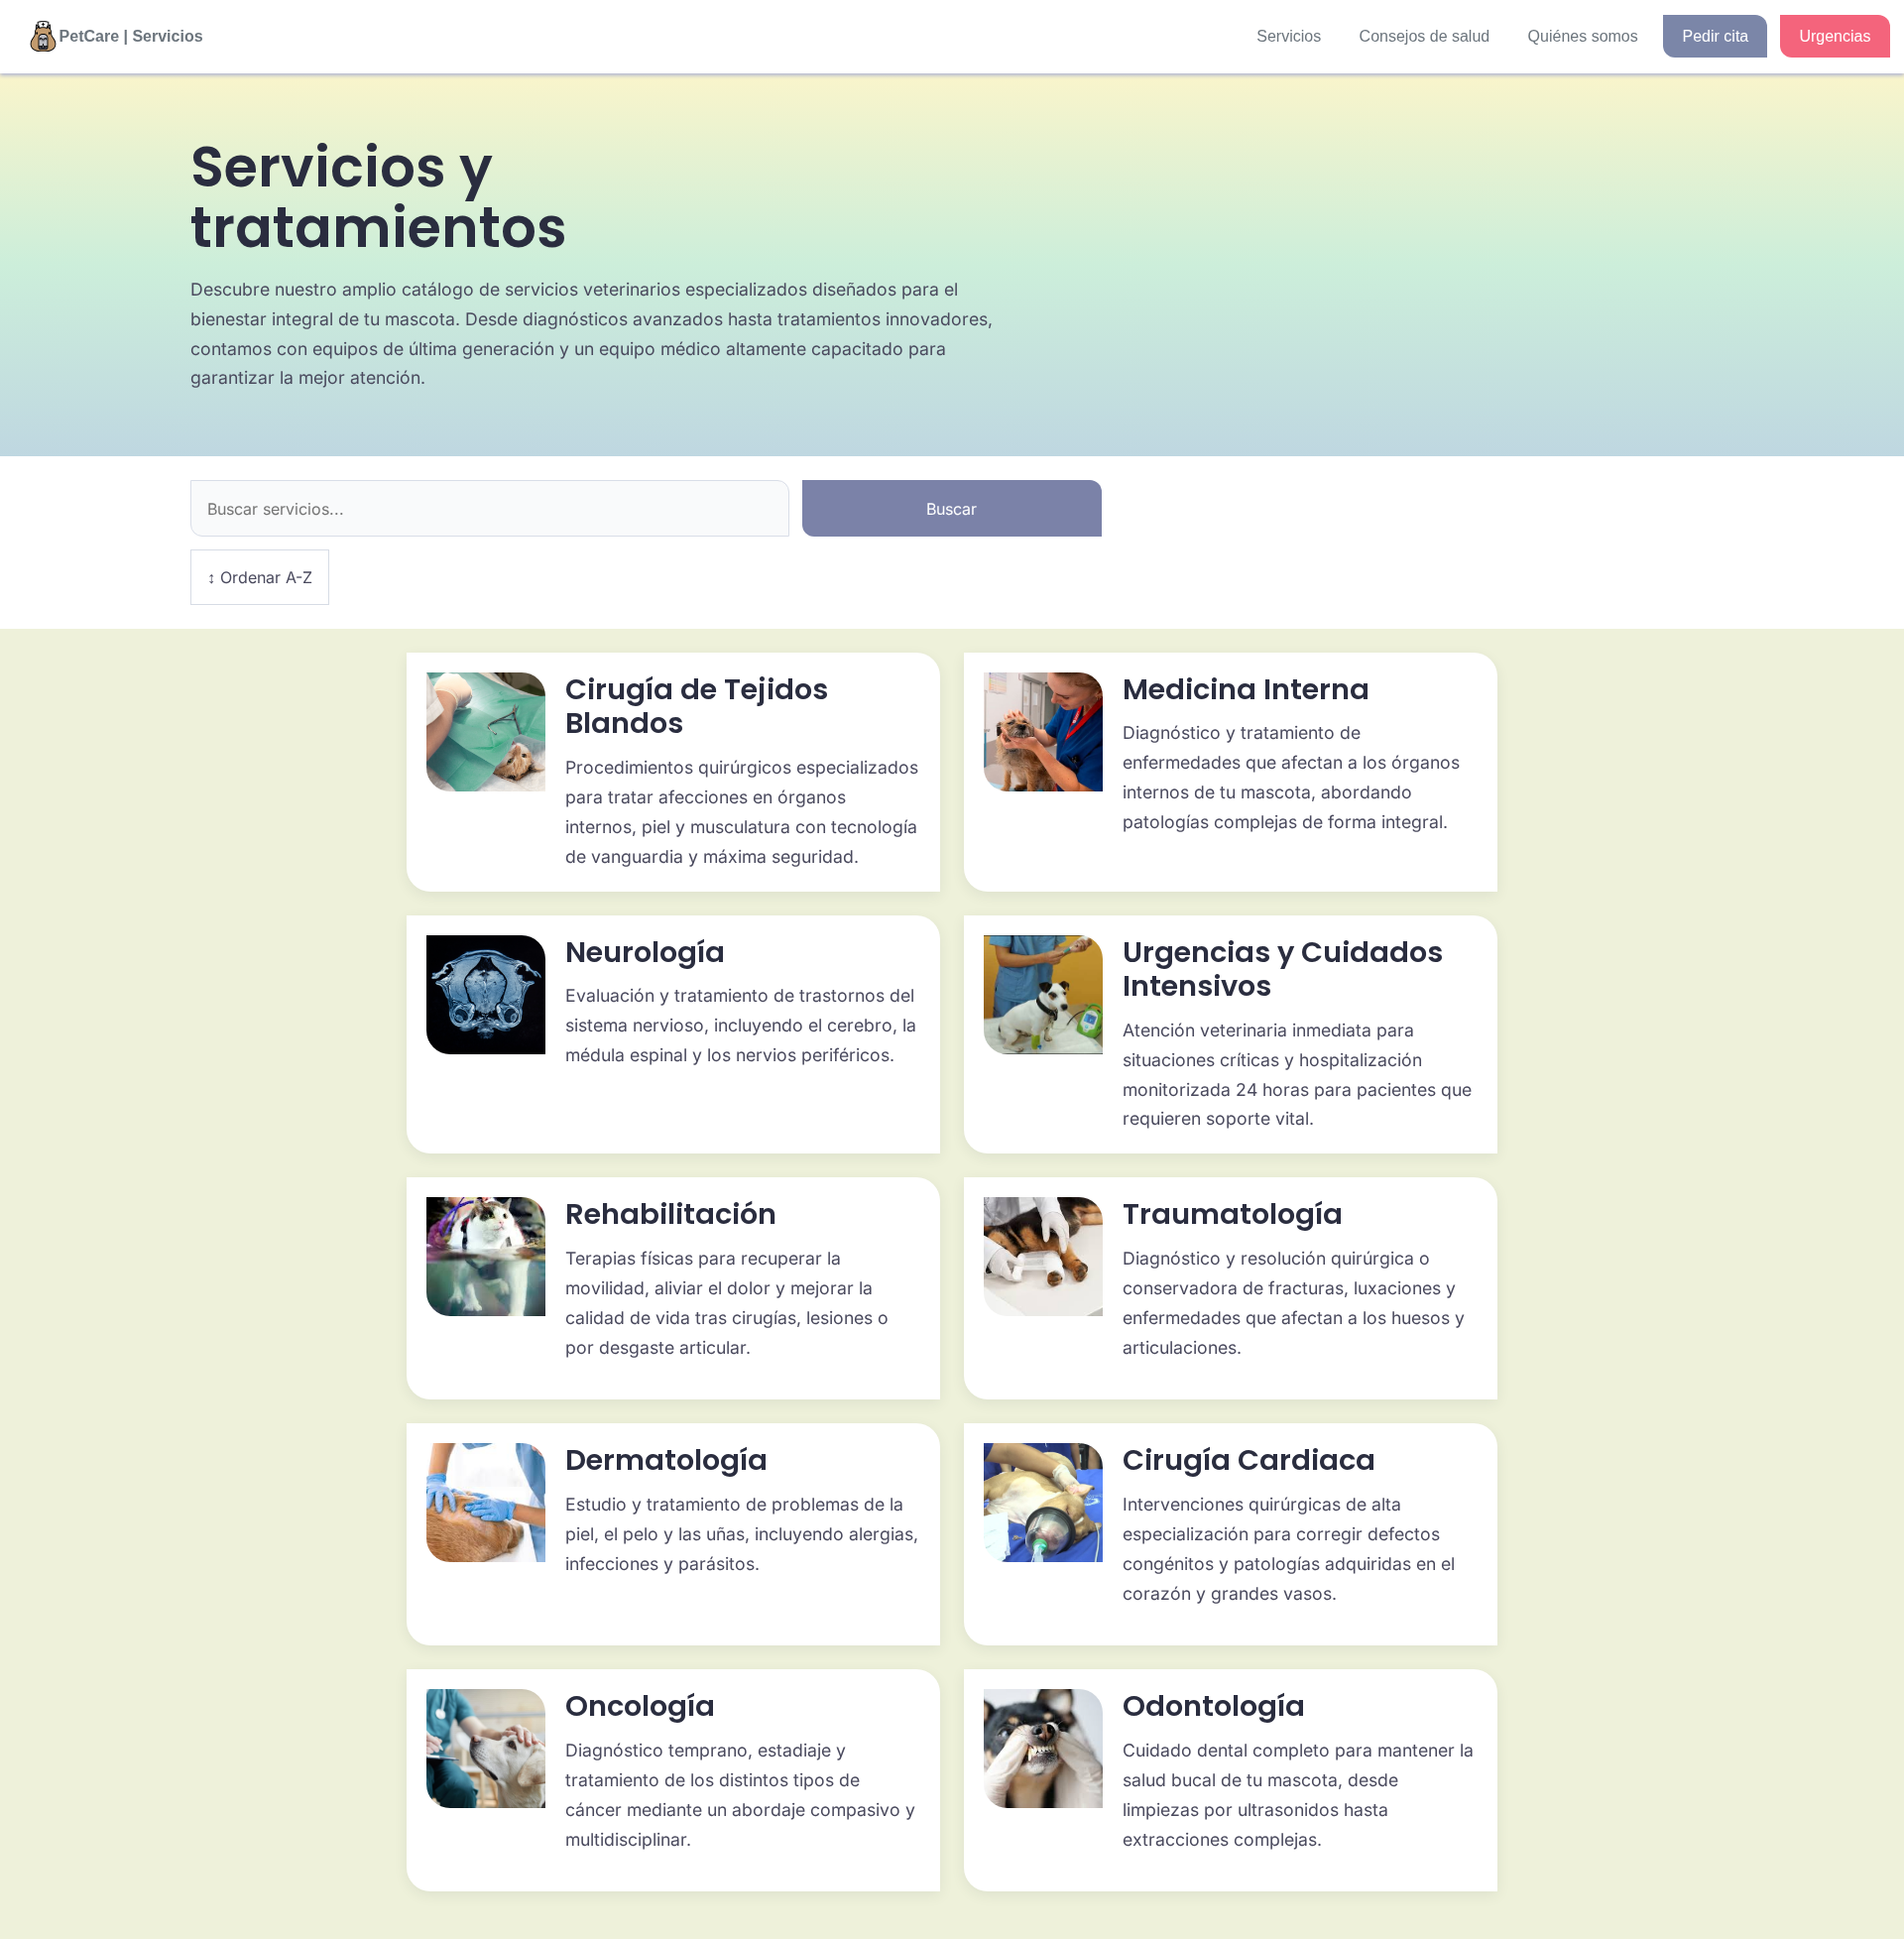
\includegraphics[width=0.85\textheight,keepaspectratio]{capturas_responsivas/servicios-desktop.png}}
\caption{Servicios: versión escritorio}
\end{figure}

\begin{figure}[H]
\centering
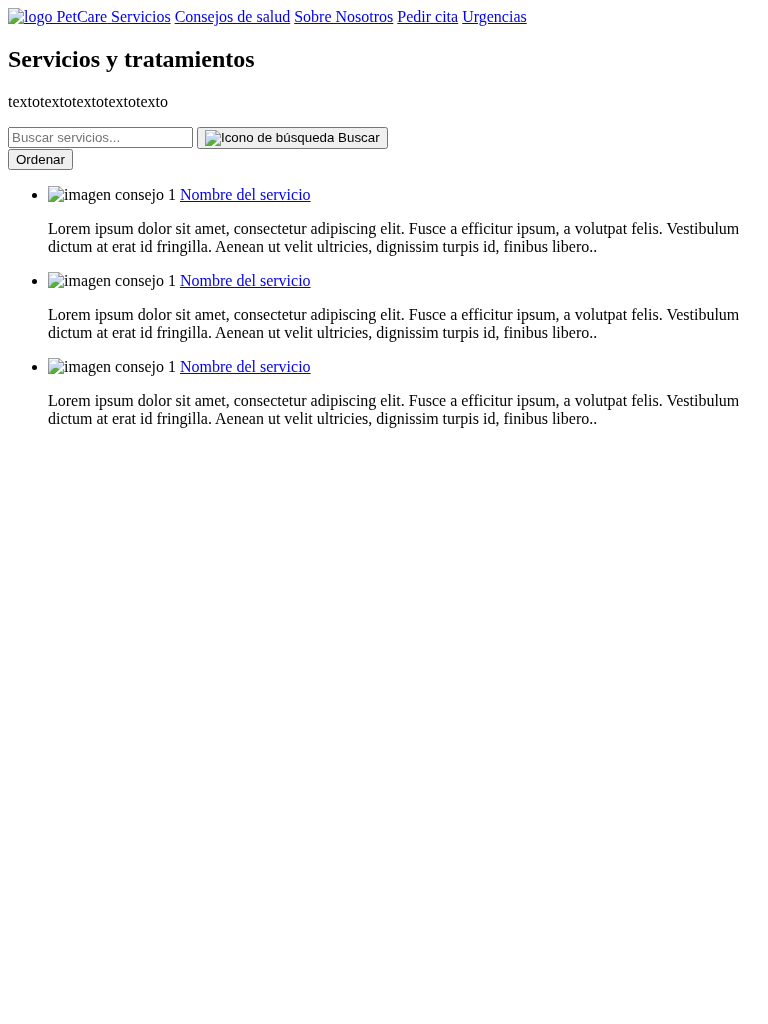
\includegraphics[width=0.65\linewidth,height=0.60\textheight,keepaspectratio]{capturas_responsivas/servicios-tablet.png}
\caption{Servicios: versión tablet}
\end{figure}

\begin{figure}[H]
\centering
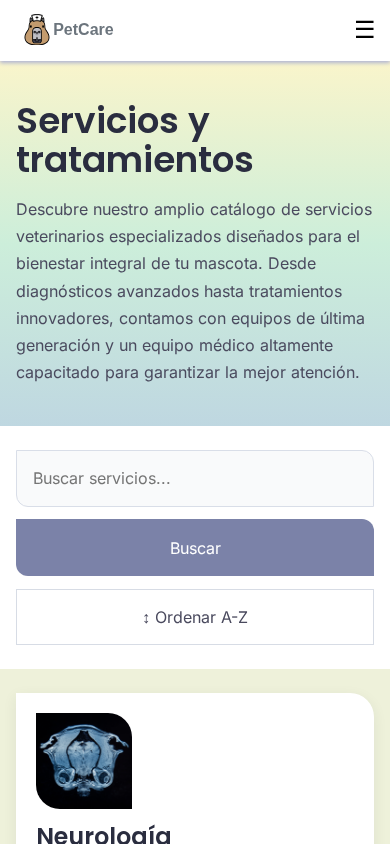
\includegraphics[width=0.38\linewidth,height=0.60\textheight,keepaspectratio]{capturas_responsivas/servicios-mobile.png}
\caption{Servicios: versión móvil}
\end{figure}

\begin{figure}[H]
\centering
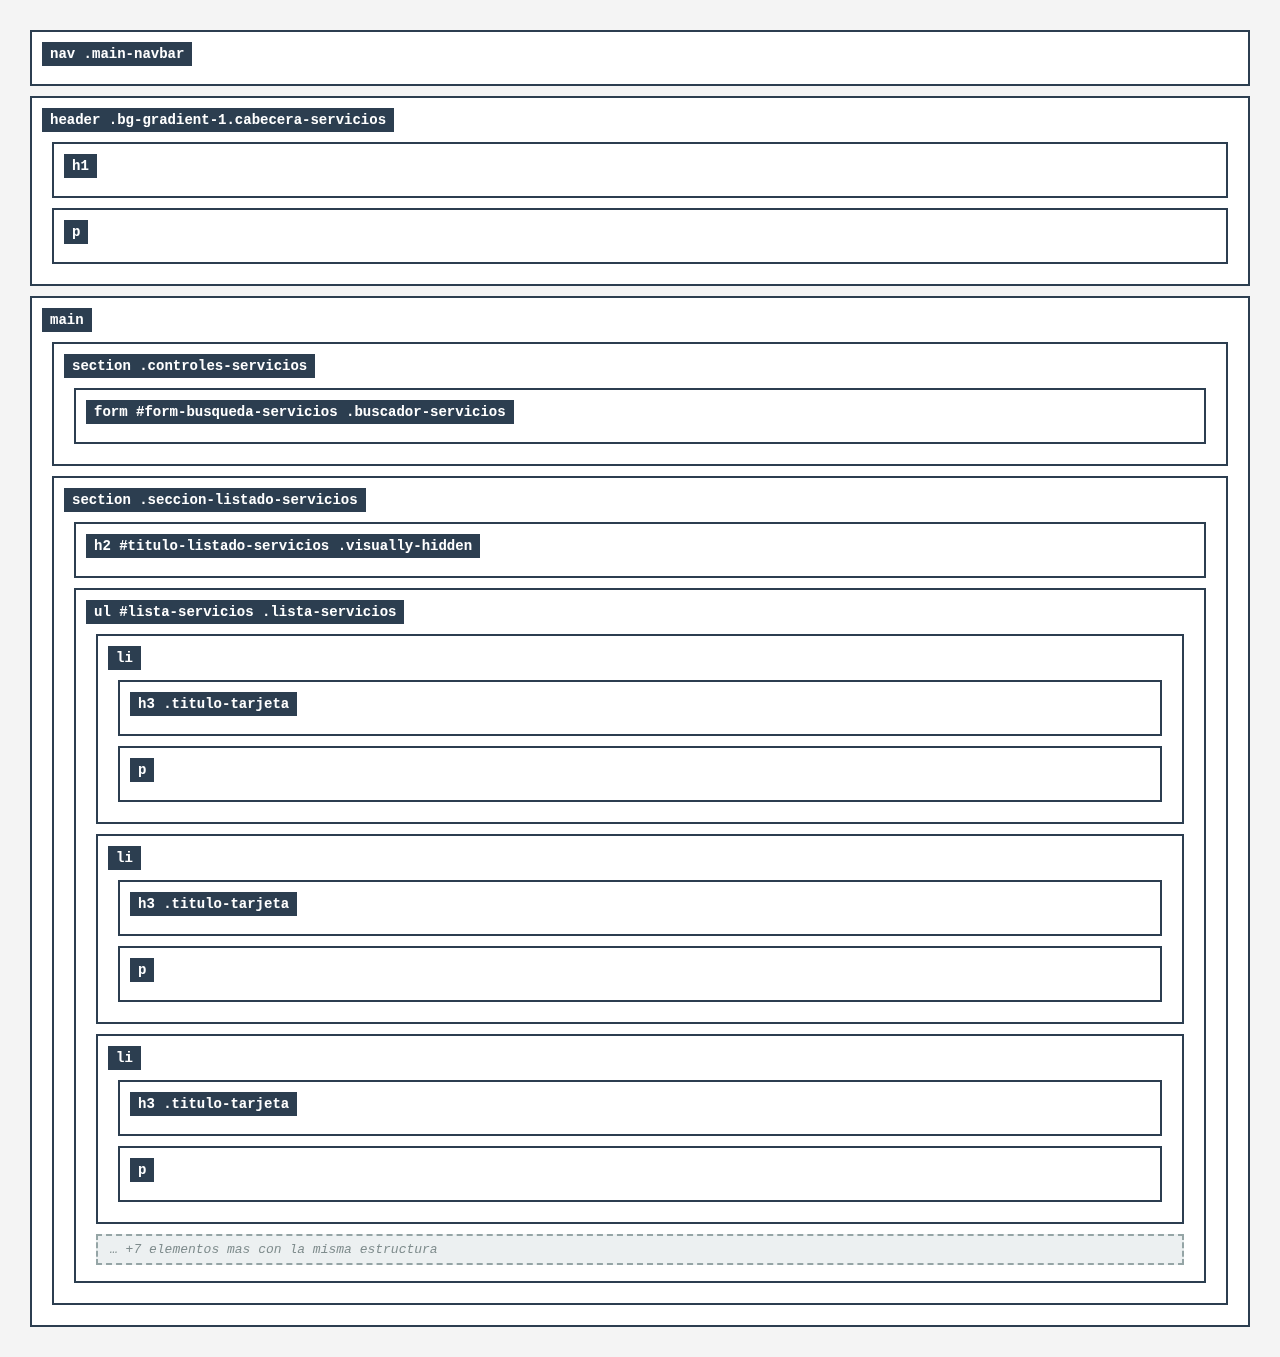
\includegraphics[width=\linewidth,height=0.85\textheight,keepaspectratio]{mapasDeEtiquetas/servicios-boxmodel-new.png}
\caption{Mapa de etiquetas actualizado (P3) --- Servicios}
\end{figure}

\clearpage

% ─────────────────────────────────────────────────────────────────────────────
\subsection{Framework Bootstrap --- Consejos de salud}
% ─────────────────────────────────────────────────────────────────────────────

En la página de consejos de salud, hemos complementado con \textbf{Bootstrap}, uno de los \textit{frameworks} de CSS más populares en el desarrollo web. Un \textit{framework} como este nos proporciona una biblioteca de estilos predefinidos y un sistema de cuadrículas robusto basado en clases de utilidad, lo que permite construir interfaces responsivas de forma mucho más ágil.

Mientras que en otras páginas hemos desarrollado nuestras propias reglas CSS desde cero, Bootstrap nos permite implementar estos componentes rápidamente y asegurar su compatibilidad entre distintos navegadores. Además, Bootstrap trabaja de forma nativa bajo el paradigma \textit{Mobile First}.

A diferencia de los métodos anteriores, donde la lógica residía en los archivos \texttt{.css}, la maquetación con Bootstrap se realiza directamente en el HTML mediante la asignación de clases compuestas a las etiquetas. Hemos aplicado las siguientes lógicas responsivas:

\begin{itemize}
\item \textbf{Estructura principal:} Envolvemos todo el contenido en un \texttt{<main class="container mt-4">}. La clase \texttt{container} centra automáticamente el contenido y aplica márgenes laterales que se adaptan a los diferentes tamaños de pantalla, mientras que \texttt{mt-4} añade un margen superior estandarizado.
\item \textbf{Navegación por pestañas (Tabs):} Utilizamos las clases \texttt{nav nav-tabs} para crear el menú visual. Para el interior de los botones, aplicamos utilidades de Flexbox integradas en Bootstrap (\texttt{d-flex flex-column align-items-center}) que nos permiten apilar perfectamente el icono del animal sobre su nombre correspondiente.
\item \textbf{Buscador adaptable (Mobile First):} En la etiqueta \texttt{<search>} aplicamos \texttt{w-100} para que el buscador ocupe todo el ancho en móviles, y \texttt{w-md-50} para que se reduzca a la mitad de la pantalla a partir de monitores medianos.
\item \textbf{Formulario fluido:} Al formulario interno le asignamos las clases \texttt{d-flex flex-column flex-md-row}. Esto es un ejemplo de responsividad mediante clases: por defecto (móviles), la barra de búsqueda y el botón se apilan verticalmente (\texttt{flex-column}). Sin embargo, a partir de pantallas medianas (\texttt{-md-}), cambian su comportamiento y se colocan uno al lado del otro en horizontal (\texttt{flex-md-row}).
\end{itemize}

A continuación, se presenta el código HTML donde se aprecia la aplicación de estas clases de utilidad:

\begin{lstlisting}[language=HTML, caption=Implementación de diseño responsivo mediante clases de Bootstrap]
<main class="container mt-4">
<ul class="nav nav-tabs justify-content-center border-0 gap-3"
id="categoria-animales" role="tablist">
<li class="nav-item" role="presentation">
<button class="nav-link d-flex flex-column align-items-center
border rounded p-3 text-muted active"
id="home-tab" data-bs-toggle="tab"
data-bs-target="#perros-tab-pane" type="button" role="tab"
aria-controls="perros-tab-pane" aria-selected="true">
<img class="consejos-tab-icon-button"
src="assets/imgs/dog-svgrepo-com.svg" alt="Icono de perro">
Perros
</button>
</li>
<!-- ... otros items omitidos por brevedad ... -->
</ul>
<search class="w-100 w-md-50 mt-4 m-auto">
<form class="d-flex flex-column flex-md-row bg-white
shadow-sm rounded-3 p-1" role="search" name="buscarClinica">
<input class="form-control me-2" type="search"
placeholder="Buscar consejos..." aria-label="Search" />
<button class="btn btn-secondary d-flex justify-content-center
p-3 ps-lg-4 pe-lg-4 borde-asimetrico" type="submit">
Buscar
</button>
</form>
</search>
<ul class="row list-unstyled justify-content-center mt-3 g-3"></ul>
</main>
\end{lstlisting}

\begin{figure}[H]
\centering
\rotatebox{90}{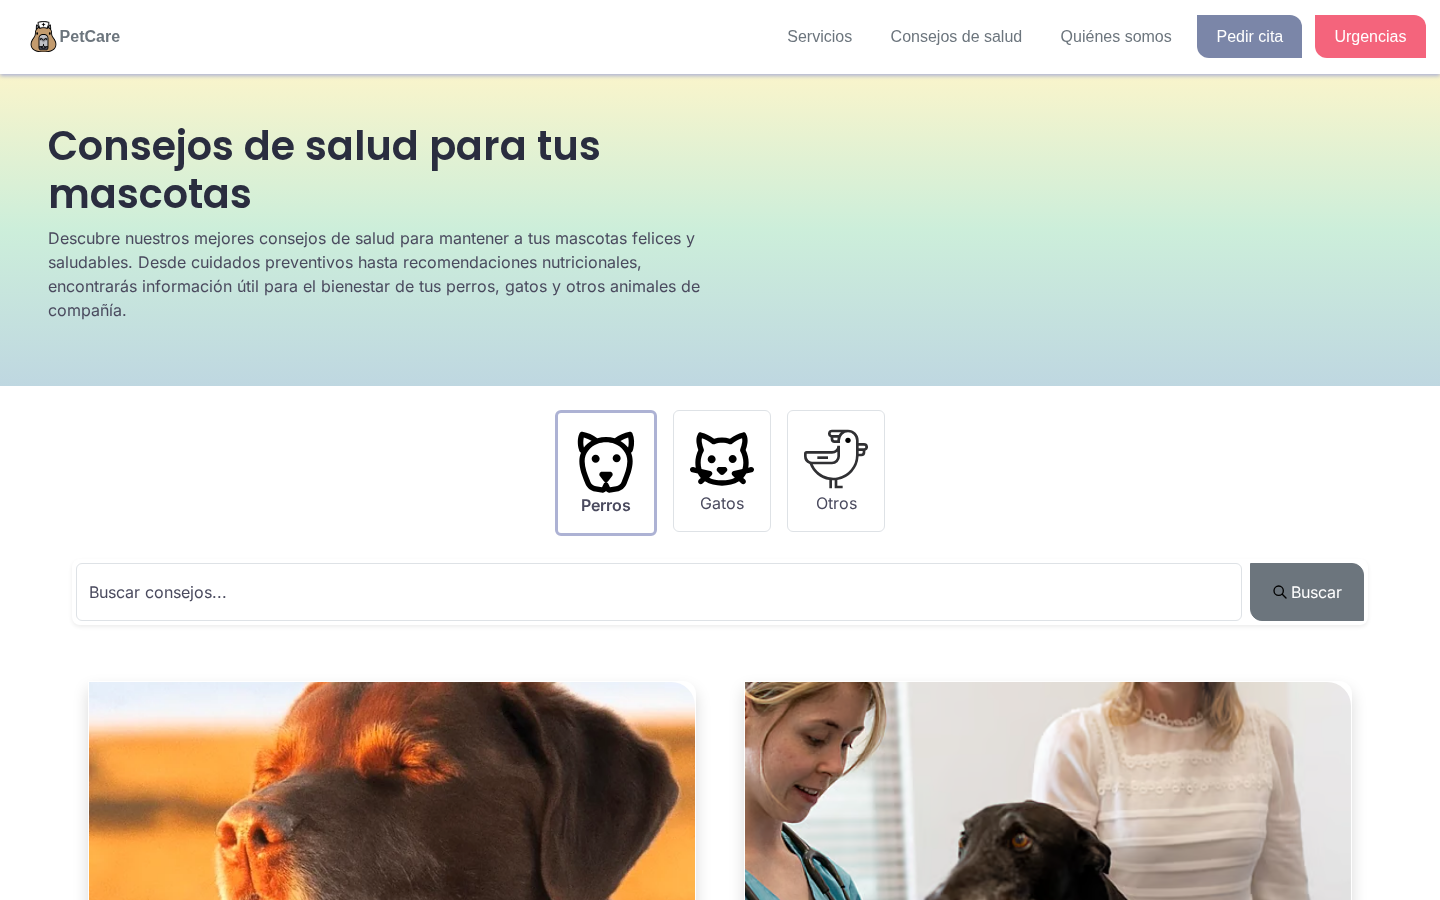
\includegraphics[width=0.85\textheight,keepaspectratio]{capturas_responsivas/consejos-desktop.png}}
\caption{Consejos de salud: versión escritorio}
\end{figure}

\begin{figure}[H]
\centering
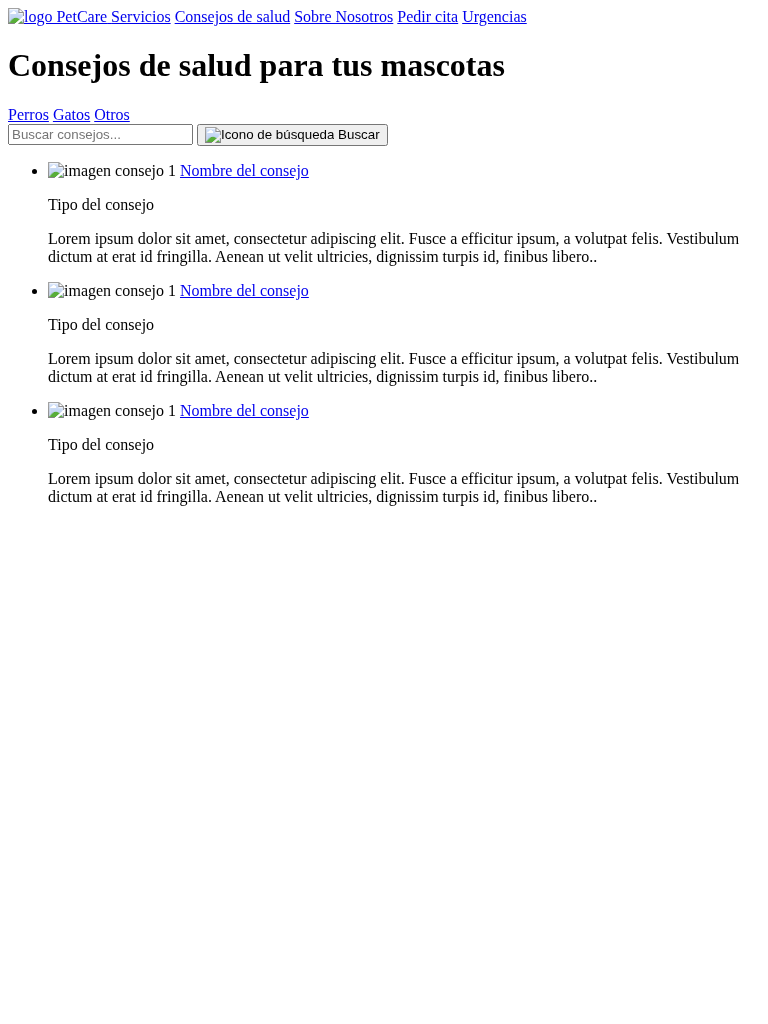
\includegraphics[width=0.65\linewidth,height=0.60\textheight,keepaspectratio]{capturas_responsivas/consejos-tablet.png}
\caption{Consejos de salud: versión tablet}
\end{figure}

\begin{figure}[H]
\centering
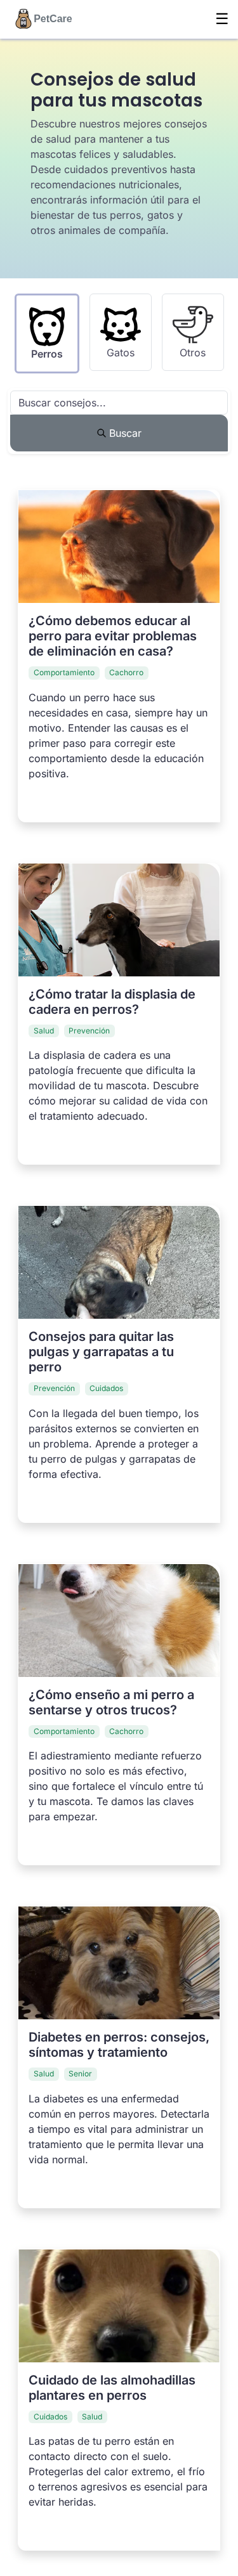
\includegraphics[width=0.38\linewidth,height=0.60\textheight,keepaspectratio]{capturas_responsivas/consejos-mobile.png}
\caption{Consejos de salud: versión móvil}
\end{figure}

\begin{figure}[H]
\centering
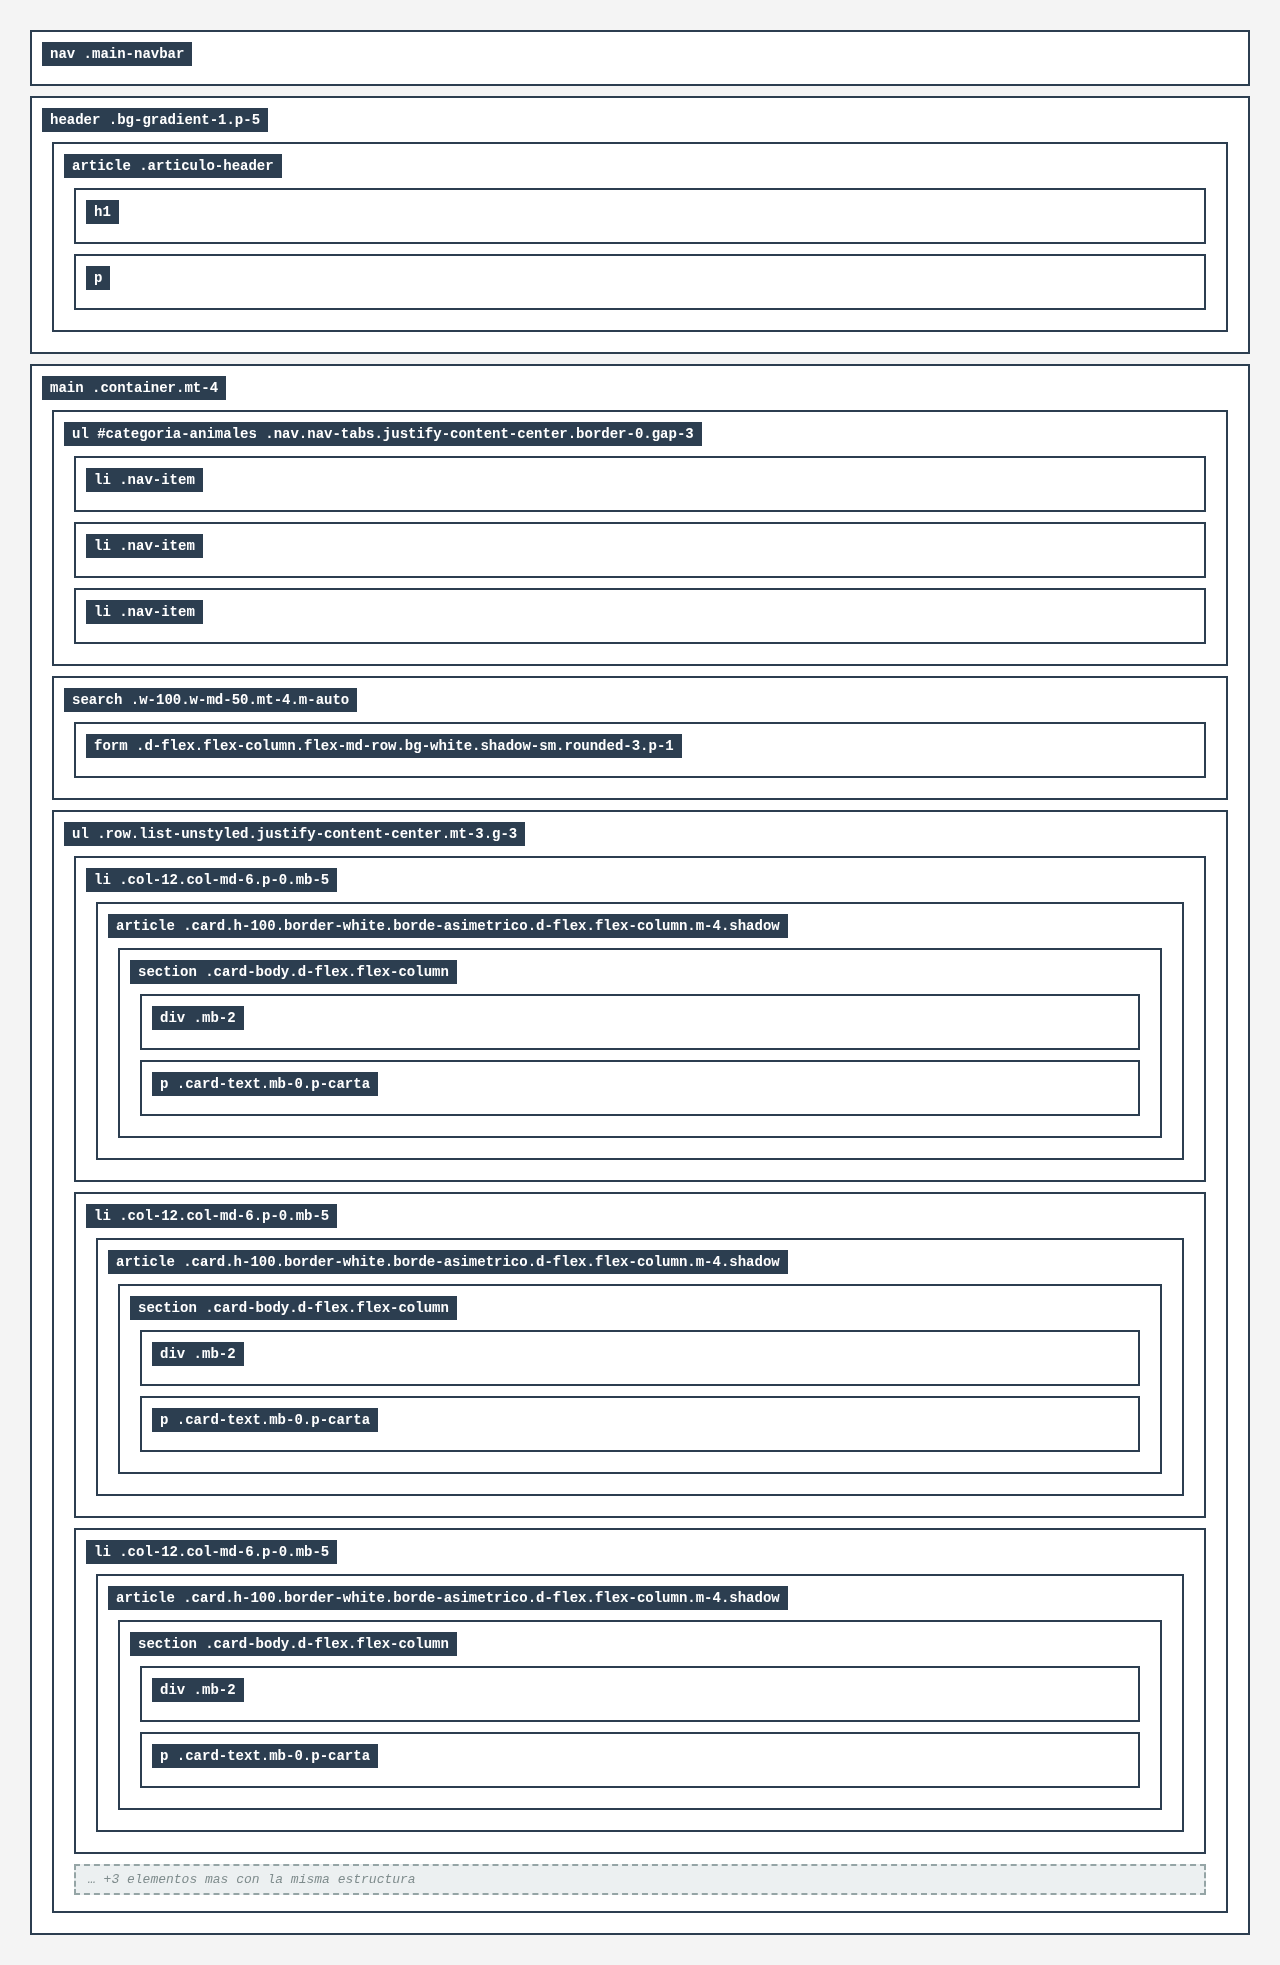
\includegraphics[width=\linewidth,height=0.85\textheight,keepaspectratio]{mapasDeEtiquetas/consejos-boxmodel-new.png}
\caption{Mapa de etiquetas actualizado (P3) --- Consejos de salud}
\end{figure}

\clearpage

% =============================================================================
\section{Práctica 4: JavaScript}
% =============================================================================

\subsection{Efectos visibles}

% ─────────────────────────────────────────────────────────────────────────────
\subsubsection{Navegación dinámica por pestañas en la página Sobre Nosotros}
% ─────────────────────────────────────────────────────────────────────────────

En la página ``Quiénes somos'', hemos implementado un sistema interactivo de pestañas. Este efecto permite al usuario alternar entre diferentes secciones de texto (Sostenibilidad, Principios, Medicina veterinaria y Por qué PetCare) pulsando sobre sus respectivos botones. Al hacer clic, el contenido inferior se actualiza instantáneamente sin necesidad de recargar la página web, y el botón pulsado se resalta visualmente para indicar en qué sección nos encontramos.

\begin{figure}[H]
    \centering
    \begin{minipage}{0.48\textwidth}
        \centering
        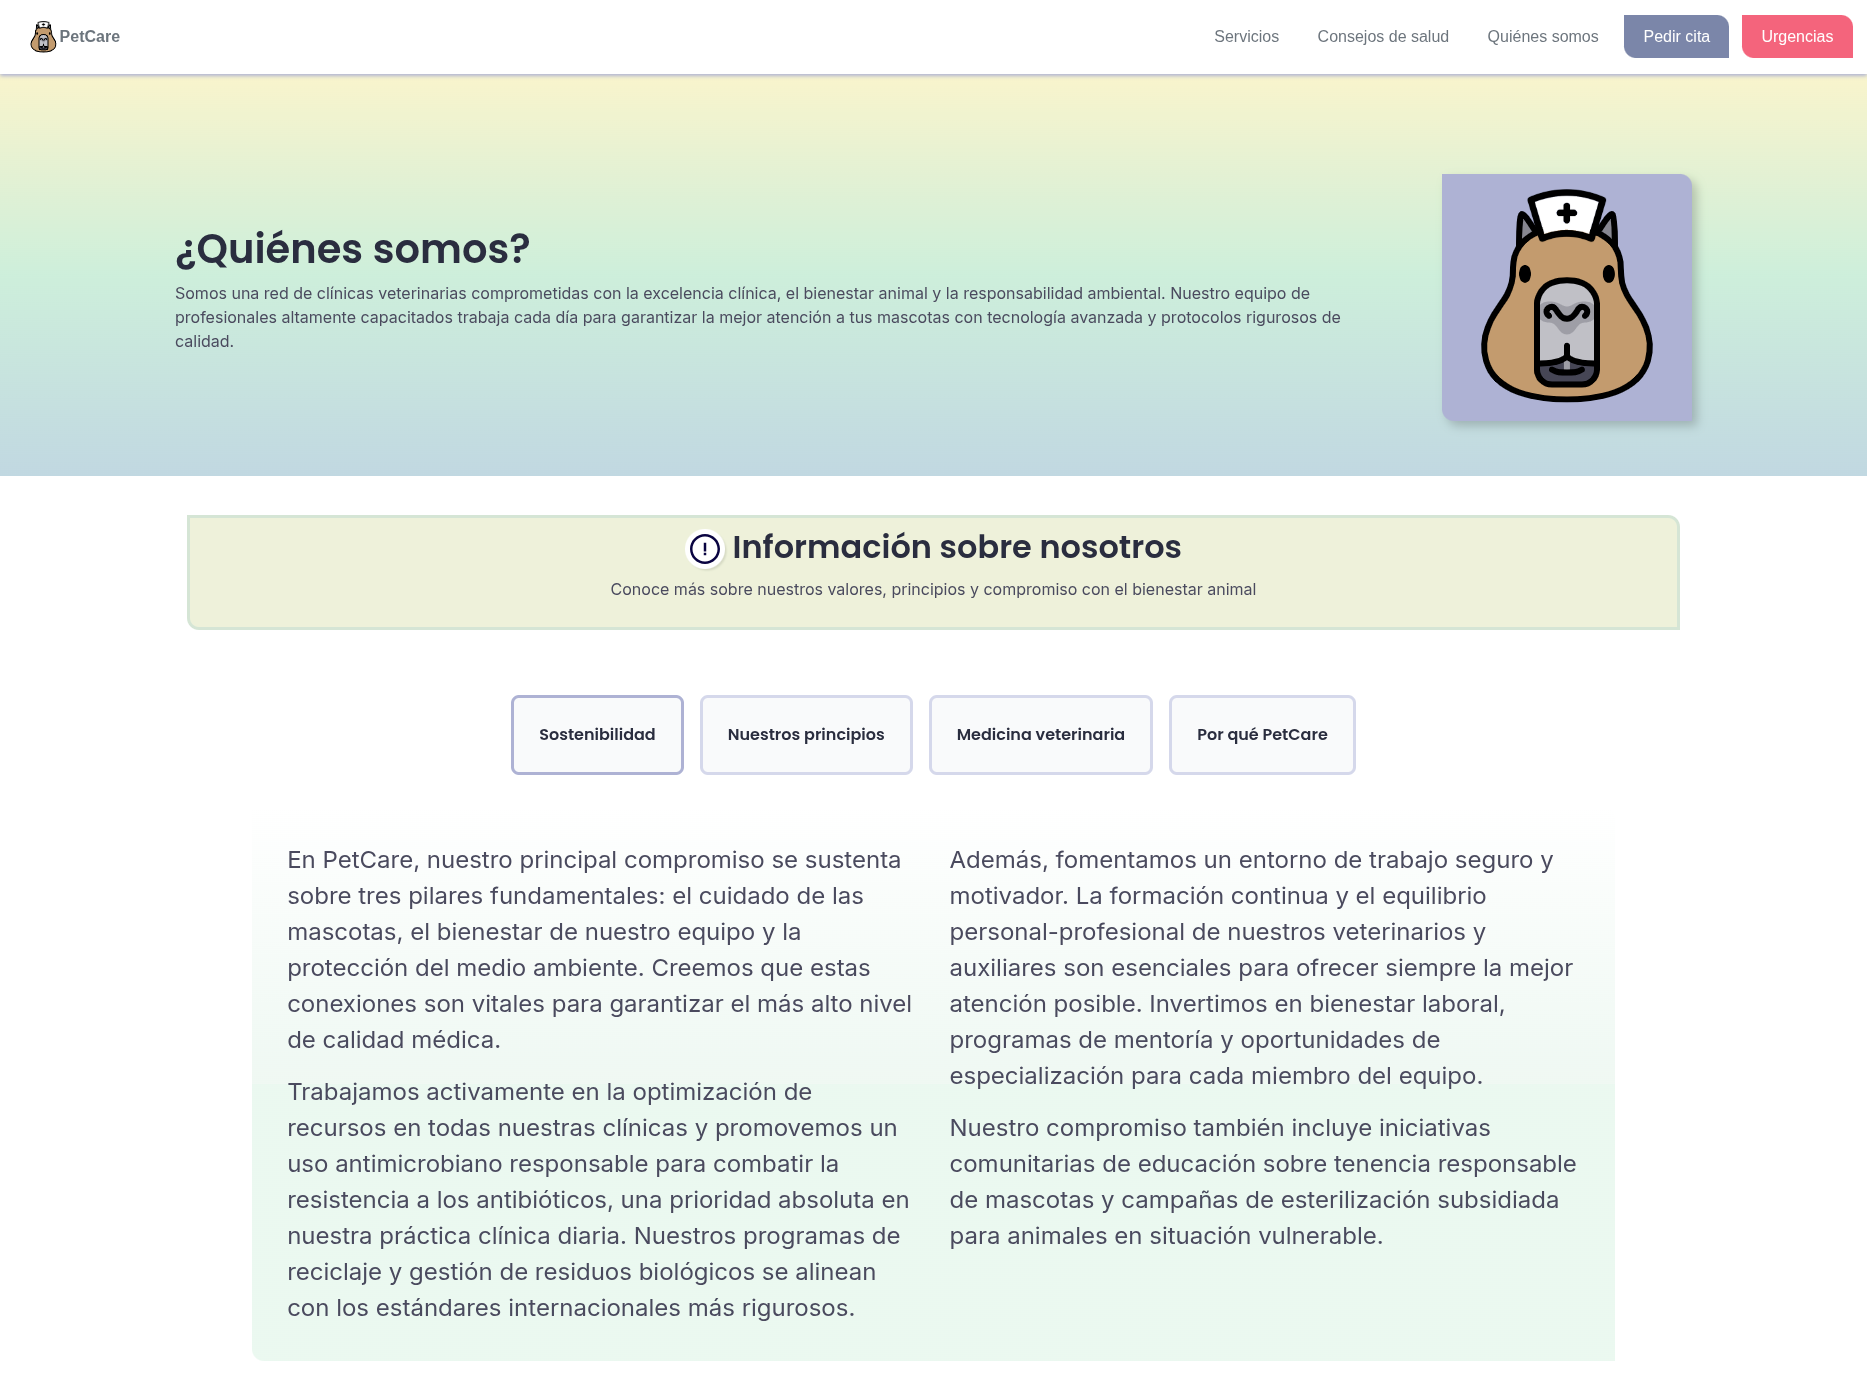
\includegraphics[width=\linewidth,keepaspectratio]{capturas_js/nav-dinamica-sobre-nosotros-1.png} % Nota: Asumo que la extensión es .png por consistencia, ajusta a .jpg si fuera necesario según tu árbol.
        \caption{Pestaña de sostenibilidad activa}
    \end{minipage}\hfill
    \begin{minipage}{0.48\textwidth}
        \centering
        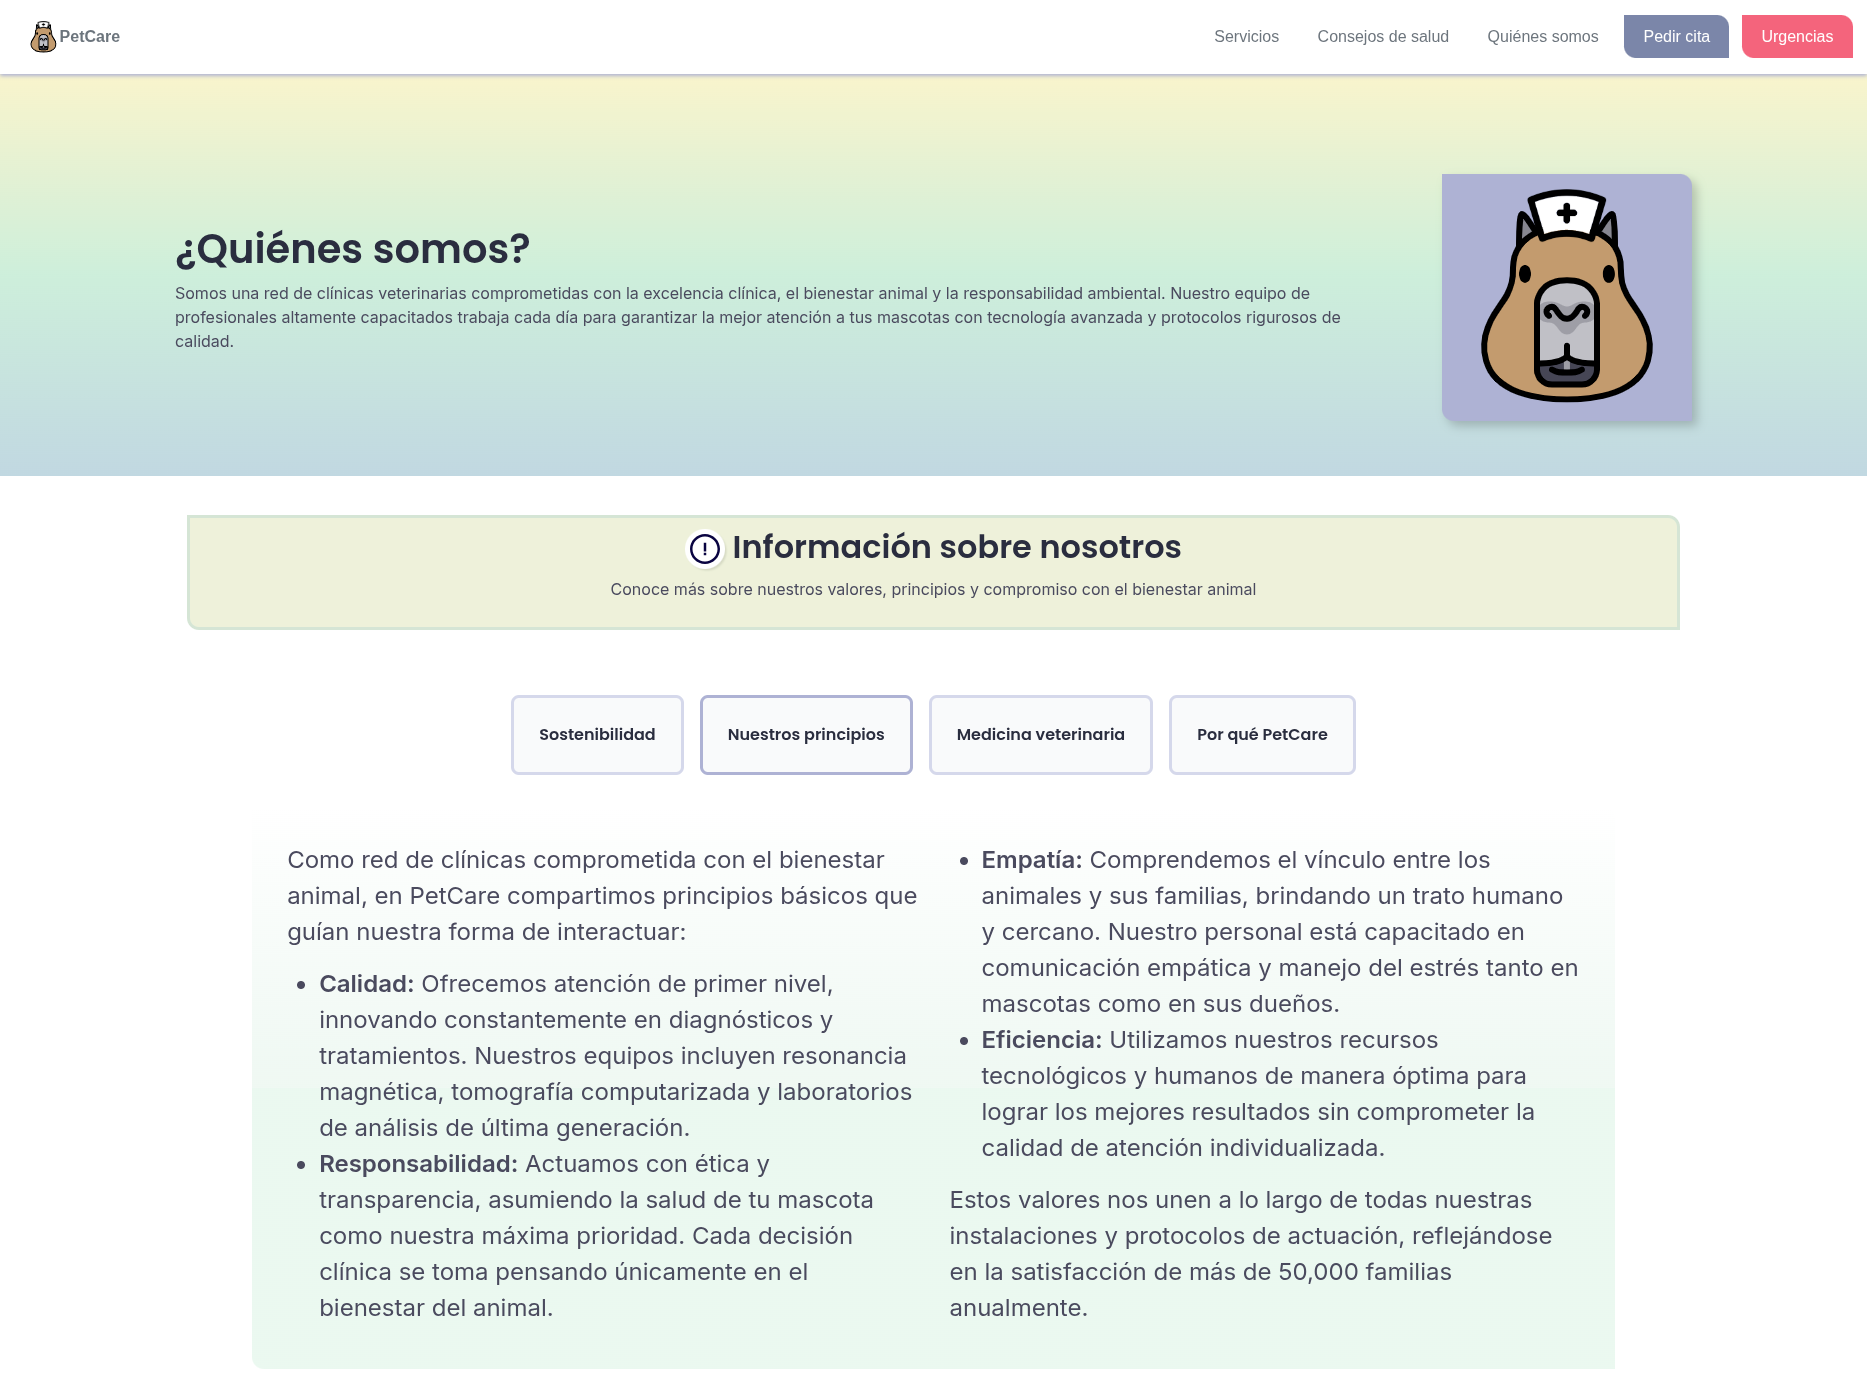
\includegraphics[width=\linewidth,keepaspectratio]{capturas_js/nav-dinamica-sobre-nosotros-2.png}
        \caption{Inyección dinámica de nuevo contenido de texto}
    \end{minipage}
\end{figure}

El funcionamiento de este efecto se basa en la interacción coordinada entre la estructura HTML y el motor de eventos de JavaScript. Para lograrlo, dividimos la lógica en las siguientes partes críticas:

\begin{itemize}
\item \textbf{Preparación del HTML:} En el documento, creamos botones (\texttt{<button>}) con la clase común \texttt{btn-pestana}. El elemento clave aquí es el atributo personalizado \texttt{data-clave}, que almacena un identificador único para cada botón (por ejemplo, \texttt{data-clave="sostenibilidad"}). Además, definimos un contenedor vacío (\texttt{<section id="area-despliegue-texto">}) que actuará como ``pizarra'' donde inyectaremos el texto.
\item \textbf{Origen de los datos:} En JavaScript, creamos un objeto constante llamado \texttt{repositorioTextos}. Este objeto actúa como un diccionario donde las claves coinciden exactamente con los valores de los atributos \texttt{data-clave} del HTML, y sus valores contienen el código HTML del texto a mostrar.
\item \textbf{Acceso al DOM:} Utilizando el método \texttt{querySelectorAll(".btn-pestana")}, capturamos todos los botones en una lista. Simultáneamente, capturamos el contenedor de destino mediante \texttt{getElementById("area-despliegue-texto")}.
\item \textbf{Manejo de Eventos (El clic):} Iteramos sobre la lista de botones usando un bucle \texttt{forEach} para asignar a cada uno un escuchador de eventos (\texttt{addEventListener}) de tipo \texttt{click}.
\item \textbf{Actualización visual y de contenido:} Cuando se dispara el evento, el código realiza dos acciones. Primero, elimina la clase CSS \texttt{activo} de todos los botones y se la añade únicamente al botón que acaba de ser pulsado (\texttt{evento.currentTarget}), actualizando así la interfaz. Segundo, lee el atributo \texttt{data-clave} de ese botón y utiliza ese valor para buscar el texto correspondiente en el \texttt{repositorioTextos}, inyectándolo finalmente en el contenedor mediante la propiedad \texttt{innerHTML}.
\end{itemize}

\begin{lstlisting}[language=HTML, caption=Estructura HTML para la botonera y el contenedor de texto]
<nav class="botones-navegacion">
<button class="btn-pestana activo" data-clave="sostenibilidad">
Sostenibilidad
</button>
<button class="btn-pestana" data-clave="principios">
Nuestros principios
</button>
<button class="btn-pestana" data-clave="medicina">
Medicina veterinaria
</button>
<button class="btn-pestana" data-clave="por_que">
Por que PetCare
</button>
</nav>
<section id="area-despliegue-texto" class="contenedor-multicol borde-asimetrico">
</section>
\end{lstlisting}

\begin{lstlisting}[language=JavaScript, caption=Lógica JavaScript para la alternancia de pestañas]
document.addEventListener("DOMContentLoaded", () => {
	// 1. Origen de datos (diccionario)
	const repositorioTextos = {
		sostenibilidad: `<p>En PetCare, nuestro principal compromiso...</p>`,
		principios: `<p>Como red de clinicas comprometida con...</p>`
		// ...
	};
	// 2. Acceso al DOM
	const botones = document.querySelectorAll(".btn-pestana");
	const contenedorDespliegue = document.getElementById("area-despliegue-texto");
	
	// 3. Estado inicial por defecto (Primera pestana activa)
	botones[0].classList.add("activo");
	contenedorDespliegue.innerHTML =
	repositorioTextos[botones[0].getAttribute("data-clave")];
	
	// 4. Asignacion de manejadores de eventos
	botones.forEach(boton => {
		boton.addEventListener("click", (evento) => {
			// Actualizacion del estado visual de la botonera
			botones.forEach(btn => btn.classList.remove("activo"));
			evento.currentTarget.classList.add("activo");
			// Recuperacion e inyeccion del contenido asociado
			const claveSeleccionada =
			evento.currentTarget.getAttribute("data-clave");
			contenedorDespliegue.innerHTML = repositorioTextos[claveSeleccionada];
		});
	});
});
\end{lstlisting}

\clearpage

% ─────────────────────────────────────────────────────────────────────────────
\subsubsection{Búsqueda dinámica de clínicas}
% ─────────────────────────────────────────────────────────────────────────────

En la página de búsqueda de clínicas, hemos desarrollado una interfaz dinámica que permite al usuario encontrar un centro adecuado sin necesidad de recargar la página web. Este sistema se compone de un buscador que filtra los resultados en tiempo real (mientras el usuario teclea), un botón para ordenar alfabéticamente, un filtro para mostrar únicamente las clínicas abiertas en el momento de la consulta, y un botón de reseteo.

Adicionalmente, la búsqueda está integrada con la página principal (\texttt{index.html}): el formulario de búsqueda de la portada captura el término introducido por el usuario y lo transmite como parámetro en la URL (\texttt{clinicas.html?clinica=\ldots}). Al cargar la página de clínicas, el script lee ese parámetro, filtra automáticamente los resultados y rellena el campo de búsqueda, cerrando así el circuito de navegación entre ambas páginas.

\begin{figure}[H]
    \centering
    \begin{minipage}{0.48\textwidth}
        \centering
        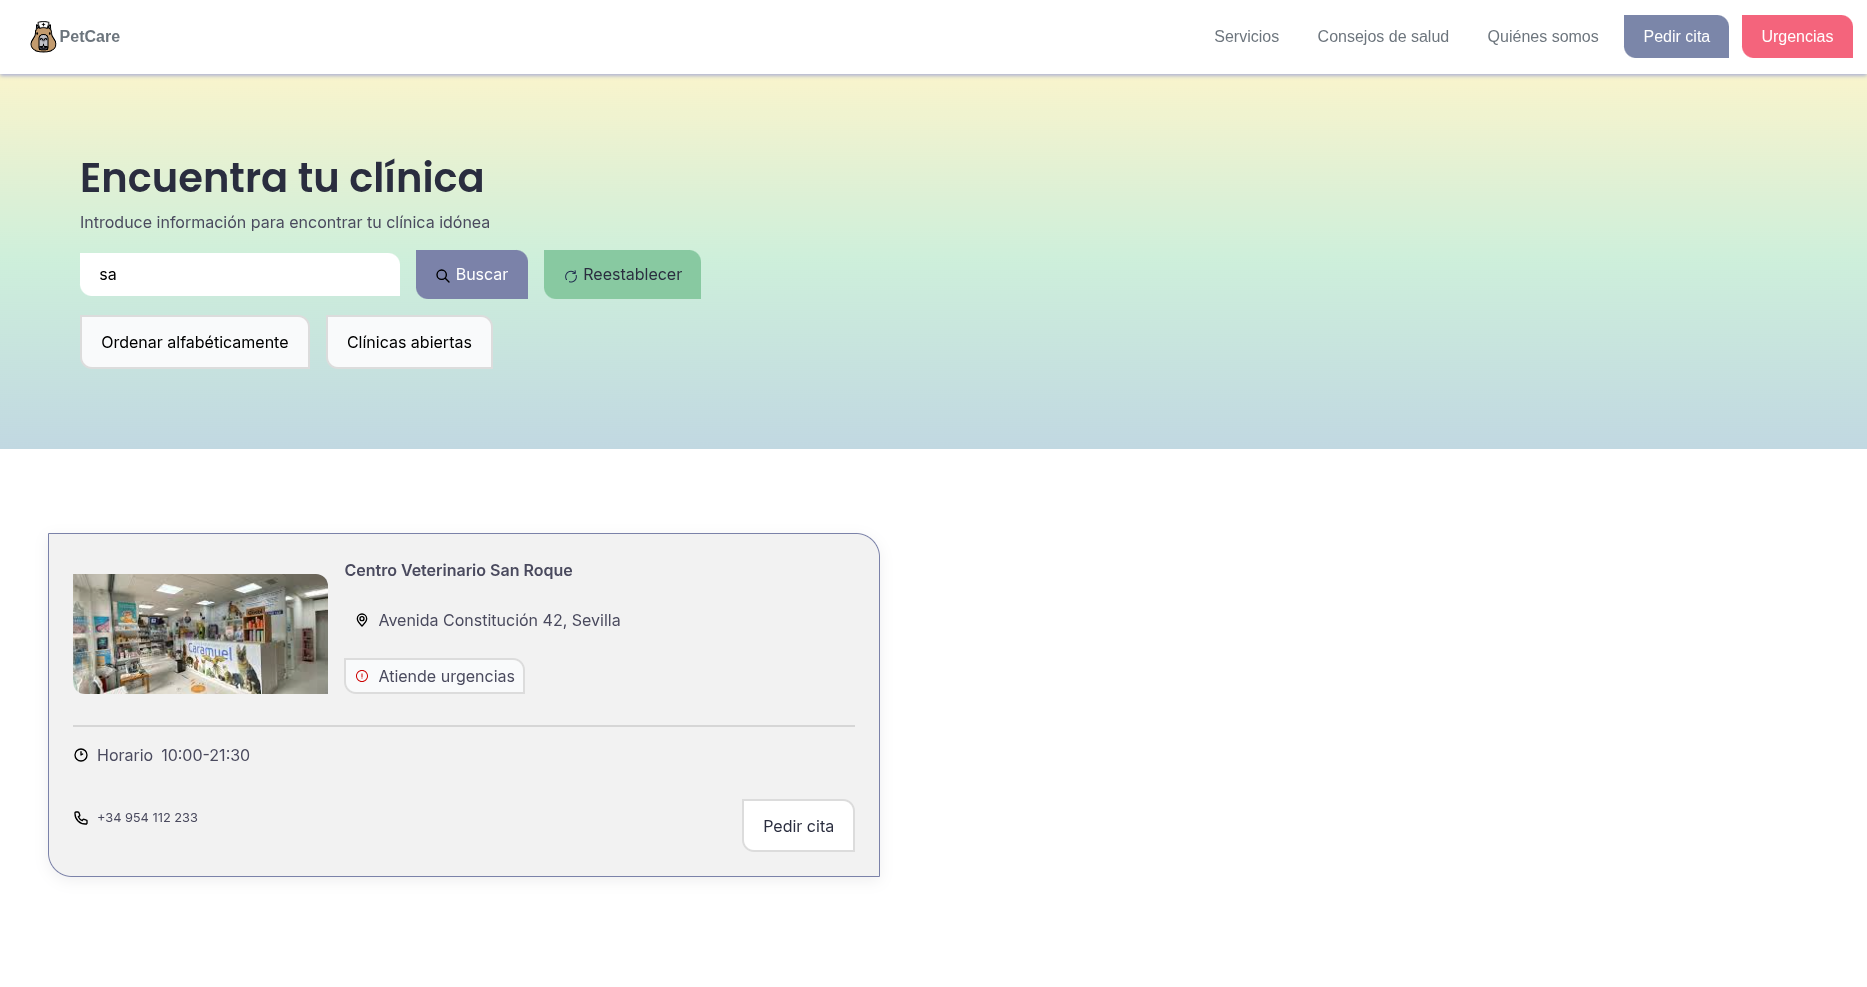
\includegraphics[width=\linewidth,keepaspectratio]{capturas_js/buqueda-dinamica-1.png}
        \caption{Vista general de clínicas (sin filtros)}
    \end{minipage}\hfill
    \begin{minipage}{0.48\textwidth}
        \centering
        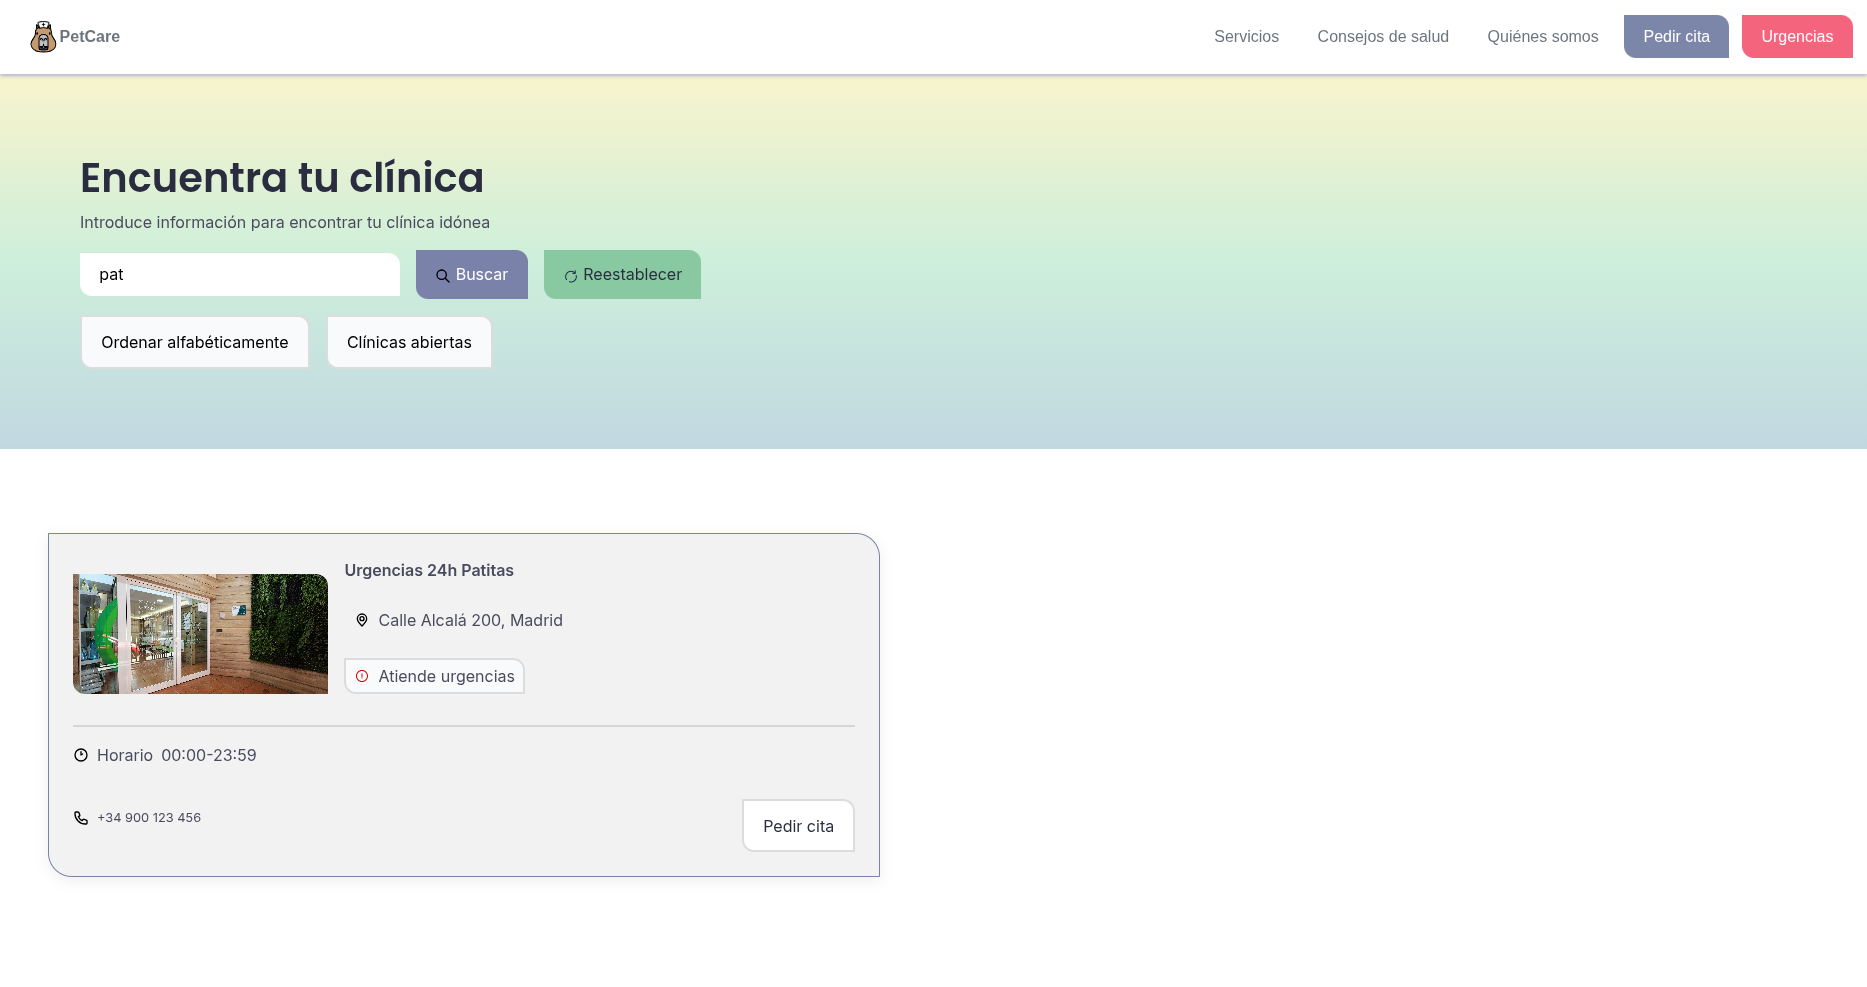
\includegraphics[width=\linewidth,keepaspectratio]{capturas_js/buqueda-dinamica-2.png}
        \caption{Renderizado condicional tras aplicar filtro}
    \end{minipage}
\end{figure}

Este sistema se basa en manipular un array de datos (cargado previamente desde un JSON) y re-renderizar la vista cada vez que el usuario interactúa con los controles. Las partes críticas del código son las siguientes:

\begin{itemize}
\item \textbf{Buscador en tiempo real:} Utilizando el objeto jQuery \texttt{\$('form[name="buscarClinica"]')}, capturamos el formulario de búsqueda. Asignamos un escuchador para el evento \texttt{input}, el cual se dispara con cada pulsación de tecla. Extraemos el valor escrito con \texttt{\$('.input-busqueda').val()} y utilizamos el método \texttt{.filter()} de ES6 sobre el array \texttt{clinicasGlobal} para obtener un nuevo array que solo contenga las clínicas cuyo nombre incluya el texto buscado.
\item \textbf{Ordenación alfabética:} Capturamos el primer botón de filtros mediante \texttt{querySelector('.contenedor-filtros li:first-child button')}. Al escuchar el evento \texttt{click}, utilizamos el método \texttt{.sort()} nativo de JavaScript. Dependiendo de una variable booleana (\texttt{ordenascendente}), comparamos los nombres de las clínicas pasados a minúsculas y alteramos el orden del array original, re-renderizando las tarjetas inmediatamente después.
\item \textbf{Filtro de clínicas abiertas:} Seleccionamos el segundo botón de la lista con \texttt{querySelectorAll}. Al recibir un \texttt{click}, instanciamos un objeto \texttt{new Date()} para obtener la hora actual del sistema del usuario, formateándola en una cadena (ej. ``14:30''). Volvemos a usar \texttt{.filter()} para separar los horarios de apertura y cierre de cada clínica y comprobar matemáticamente si la hora actual se encuentra dentro de ese rango.
\item \textbf{Integración con la portada (parámetro URL):} Al cargar la página, el script lee el parámetro \texttt{clinica} de la URL mediante \texttt{new URLSearchParams(window.location.search)}. Si existe, pre-filtra el array y rellena el campo de búsqueda automáticamente, enlazando la búsqueda iniciada desde \texttt{index.html} con los resultados de \texttt{clinicas.html}.
\item \textbf{Reseteo y renderizado:} El botón ``Reestablecer'' recarga limpiamente el documento a través de un simple enlace HTML (\texttt{href="clinicas.html"}). Para redibujar la pantalla tras cada filtro, la función \texttt{renderizarTarjetas()} vacía el contenedor utilizando el método \texttt{.empty()} de jQuery, clona la etiqueta \texttt{<template>} por cada clínica filtrada, e inyecta los nuevos nodos usando \texttt{.append()}.
\end{itemize}

\begin{lstlisting}[language=HTML, caption=Estructura HTML del buscador y controles de filtrado]
<search class="contenedor-busqueda">
<form name="buscarClinica" class="formulario-busqueda">
<input class="boton input-busqueda borde-asimetrico" type="search"
placeholder="Encuentra tu clinica..." name="clinica">
<button class="boton boton-buscar borde-asimetrico">Buscar</button>
</form>
<a href="clinicas.html"
class="boton boton-reset filtro borde-asimetrico">Reestablecer</a>
<menu class="contenedor-filtros">
<li><button class="boton borde-asimetrico filtro">
Ordenar alfabeticamente</button></li>
<li><button class="boton borde-asimetrico filtro">
Clinicas abiertas</button></li>
</menu>
</search>
\end{lstlisting}

\begin{lstlisting}[language=JavaScript, caption=Lógica JS para búsqueda en tiempo real y filtrado de horarios]
// 1. Buscador en tiempo real (uso de jQuery y evento 'input')
function inicializarBuscador() {
	let formbusqueda = $('form[name="buscarClinica"]');
	let funcbusqueda = (e) => {
		e.preventDefault();
		let txt = $('.input-busqueda').val().toLowerCase().trim();
		let clinicasFiltradas = clinicasGlobal.filter(clinica =>
		clinica.nombre.toLowerCase().includes(txt)
		);
		renderizarTarjetas(clinicasFiltradas);
	};
	formbusqueda.on('input', funcbusqueda);
}

// 2. Filtro de Clinicas abiertas (Manejo de fechas)
function inicializarHorario() {
	let horariosencendido = false;
	let btn = document.querySelectorAll('.contenedor-filtros li button')[1];
	btn.addEventListener("click", (e) => {
		e.preventDefault();
		horariosencendido = !horariosencendido;
		if (horariosencendido) {
			let fechahoy = new Date();
			let hora = fechahoy.getHours().toString().padStart(2, '0');
			let minutos = fechahoy.getMinutes().toString().padStart(2, '0');
			let horahoytexto = hora + ":" + minutos;
			let clinicasFiltradas = clinicasGlobal.filter(clinica => {
				let partes = clinica.horario.split("-");
				let abre = partes[0].trim();
				let cierra = partes[1].trim();
				return horahoytexto >= abre && horahoytexto <= cierra;
			});
			renderizarTarjetas(clinicasFiltradas);
		} else {
			renderizarTarjetas(clinicasGlobal);
		}
	});
}
\end{lstlisting}

\clearpage

% ─────────────────────────────────────────────────────────────────────────────
\subsubsection{Rotación dinámica de consejos aleatorios en la página de inicio}
% ─────────────────────────────────────────────────────────────────────────────

En la página principal, hemos implementado una sección de ``Consejos destacados'' 
que se actualiza de forma automática y autónoma. El sistema selecciona dos consejos 
de salud al azar y los muestra en pantalla. 
Cada 10 segundos, estos consejos rotan, dando paso a dos nuevos 
consejos mediante una transición de fundido. 
Esto es funcionalmente equivalente a un carrusel de consejos aleatorios.

\begin{figure}[H]
    \centering
    \begin{minipage}{0.48\textwidth}
        \centering
        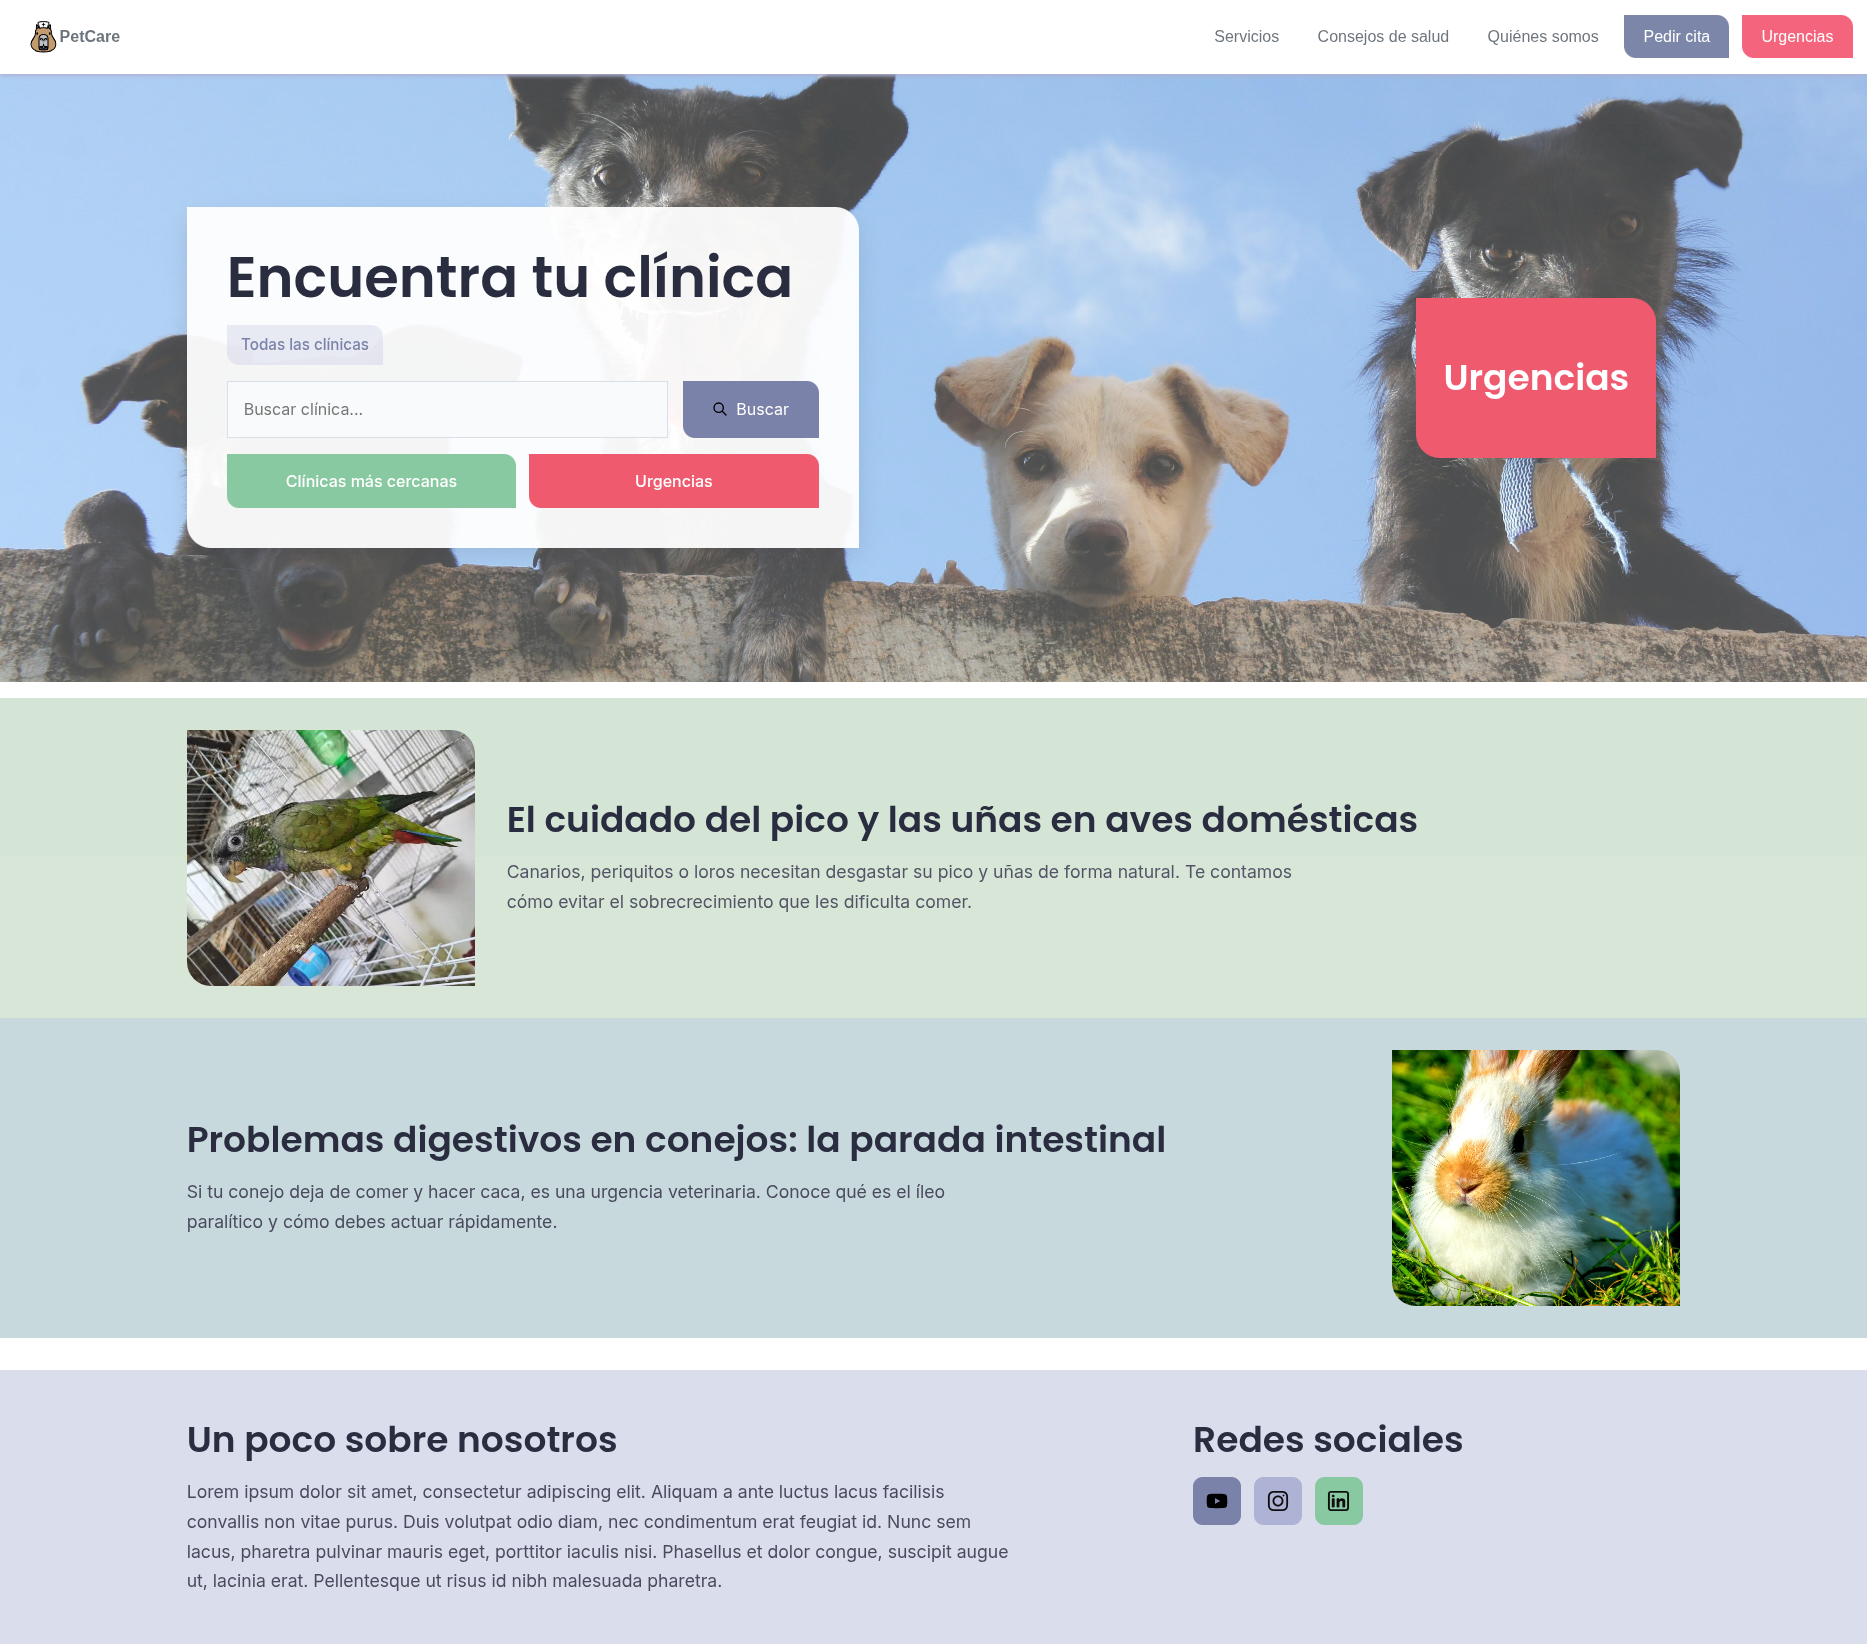
\includegraphics[width=\linewidth,keepaspectratio]{capturas_js/consejos-dinamicos-1.png}
        \caption{Estado inicial de los consejos dinámicos}
    \end{minipage}\hfill
    \begin{minipage}{0.48\textwidth}
        \centering
        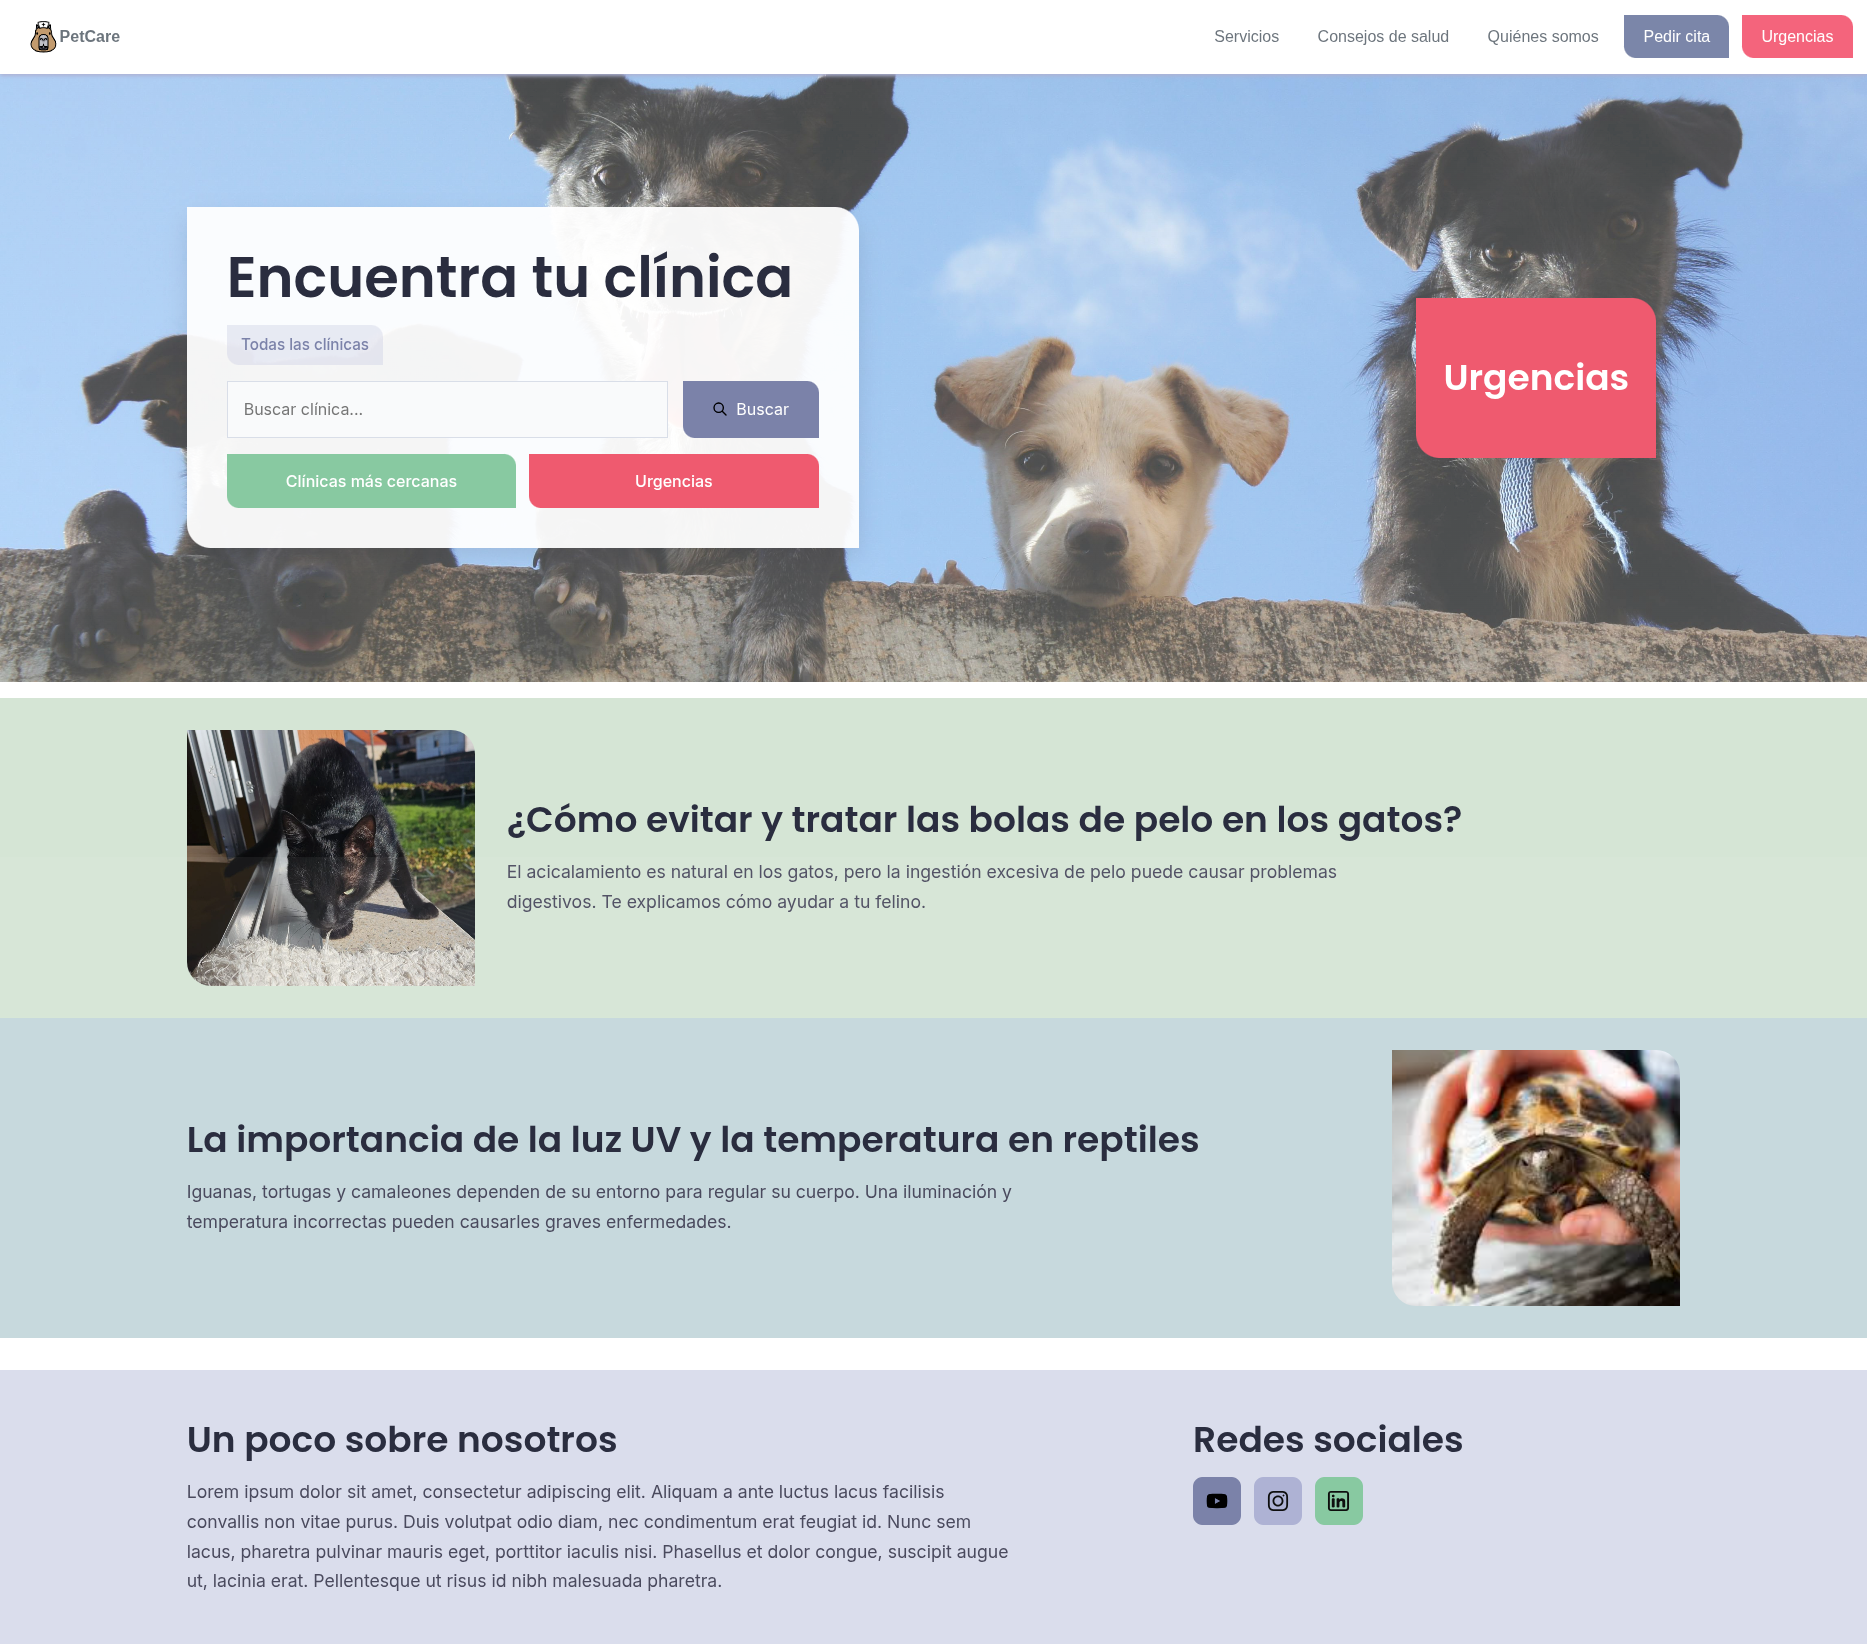
\includegraphics[width=\linewidth,keepaspectratio]{capturas_js/consejos-dinamicos-2.png}
        \caption{Estado tras el ciclo de actualización}
    \end{minipage}
\end{figure}


Este efecto combina el uso de temporizadores nativos de JavaScript, lógica matemática para la aleatoriedad y manipulación asíncrona del DOM. Las partes críticas del código son:

\begin{itemize}
\item \textbf{Inicialización y Temporizador:} Una vez cargados los datos desde el servidor, se invoca la función \texttt{actualizarConsejosIndex()} para la primera renderización. Inmediatamente después, utilizamos el método \texttt{setInterval(actualizarConsejosIndex, 10000)}, el cual programa la ejecución repetitiva de esta función cada 10.000 milisegundos (10 segundos).
\item \textbf{Lógica de Aleatoriedad:} Para garantizar que los consejos mostrados varían, generamos índices aleatorios utilizando \texttt{Math.random()} combinado con \texttt{Math.floor()} para redondear a números enteros. Implementamos un bucle \texttt{do...while} que asegura que el segundo índice (\texttt{indice2}) nunca sea exactamente igual al primero (\texttt{indice1}), evitando así mostrar el mismo consejo duplicado en pantalla.
\item \textbf{Transiciones y Manipulación del DOM:} En la función \texttt{renderizarConsejos()}, capturamos el contenedor principal mediante \texttt{getElementById("contenedor-consejos-index")}. Para crear el efecto visual de transición, primero añadimos una clase CSS \texttt{fade-out} al contenedor. Utilizamos \texttt{setTimeout()} para pausar la ejecución de JavaScript durante 300ms (el tiempo que tarda la animación CSS en ocultar el bloque).
\item \textbf{Inyección con Template Literals (ES6):} Una vez oculto el contenedor, lo vaciamos (\texttt{innerHTML = ""}) y recorremos los dos nuevos consejos con un \texttt{forEach}. Utilizamos la sintaxis de plantillas de cadena (\textit{Template Literals}) introducida en ES6 (usando comillas invertidas) para estructurar el HTML e inyectar directamente las variables (como \texttt{\$\{consejo.titulo\}}) de forma limpia.
\end{itemize}

\begin{lstlisting}[language=HTML, caption=Contenedor HTML preparado para la inyección dinámica]
<main>
<section class="consejos-home" aria-labelledby="consejos-home-titulo">
<h2 id="consejos-home-titulo" class="visually-hidden">
Consejos destacados
</h2>
<div id="contenedor-consejos-index"></div>
</section>
</main>
\end{lstlisting}

\begin{lstlisting}[language=JavaScript, caption=Lógica JS completa de index.js: carga de datos{,} buscador de portada{,} aleatoriedad y transiciones]
// 1. Carga de datos y temporizador ciclico (setInterval)
let consejosGlobal = [];
let intervaloConsejos;

document.addEventListener("DOMContentLoaded", () => {
	fetch("assets/json/consejos.json")
		.then(respuesta => respuesta.json())
		.then(datos => {
			consejosGlobal = datos.consejos;
			actualizarConsejosIndex();
			intervaloConsejos = setInterval(actualizarConsejosIndex, 10000);
		})
		.catch(error => console.error("Error al cargar consejos:", error));

	inicializarBuscadorClinicas();
});

// Buscador de la portada: redirige a clinicas.html con el termino como parametro URL
function inicializarBuscadorClinicas() {
	const formularioBusqueda = document.querySelector(".contenedor-portada-formulario");
	if (formularioBusqueda) {
		formularioBusqueda.addEventListener("submit", (e) => {
			e.preventDefault();
			const inputBusqueda = formularioBusqueda.querySelector('input[type="search"]');
			const termino = inputBusqueda.value.trim();
			if (termino) {
				window.location.href = `clinicas.html?clinica=${encodeURIComponent(termino)}`;
			}
		});
	}
}

// 2. Logica matematica de aleatoriedad
function actualizarConsejosIndex() {
	if (consejosGlobal.length < 2) return;
	let indice1 = Math.floor(Math.random() * consejosGlobal.length);
	let indice2;
	do {
		indice2 = Math.floor(Math.random() * consejosGlobal.length);
	} while (indice1 === indice2);
	renderizarConsejos([consejosGlobal[indice1], consejosGlobal[indice2]]);
}

// 3. Transiciones y ES6 Template Literals
function renderizarConsejos(listaConsejos) {
	let contenedor = document.getElementById("contenedor-consejos-index");
	contenedor.classList.add("fade-out");
	setTimeout(() => {
		contenedor.innerHTML = "";
		listaConsejos.forEach((consejo, indice) => {
			let dir = indice === 0
				? "tarjeta-servicio-inicio--imagen-izquierda"
				: "tarjeta-servicio-inicio--imagen-derecha";
			let htmlContenido = `
				<a href="consejo-especifico.html?id=${consejo.id}"
				   class="consejo-home-enlace">
				    <article class="tarjeta-servicio-inicio ${dir}">
				        <figure class="tarjeta-servicio-inicio-imagen">
				            <img src="${consejo.imagen}" class="borde-asimetrico-2"
				                 alt="${consejo.titulo}">
				        </figure>
				        <section class="tarjeta-servicio-inicio-texto">
				            <h3>${consejo.titulo}</h3>
				            <p>${consejo.preview}</p>
				        </section>
				    </article>
				</a>`;
			contenedor.innerHTML += htmlContenido;
		});
		contenedor.classList.remove("fade-out");
		contenedor.classList.add("fade-in");
		setTimeout(() => contenedor.classList.remove("fade-in"), 500);
	}, 300);
}
\end{lstlisting}

\clearpage

% ─────────────────────────────────────────────────────────────────────────────
\subsubsection{Autocompletado dinámico del nombre de la clínica en pedir cita}
% ─────────────────────────────────────────────────────────────────────────────

Hemos implementado un sistema de persistencia de datos a corto plazo que conecta la página de Clínicas con la ventana modal del formulario de citas. Cuando el usuario hace clic en el botón ``Pedir cita'' de una tarjeta específica, el formulario modal se abre mostrando automáticamente el nombre exacto de la clínica seleccionada y su ubicación en la cabecera, evitando que el usuario tenga que introducir o recordar esta información.

\begin{figure}[H]
    \centering
    \begin{minipage}{0.48\textwidth}
        \centering
        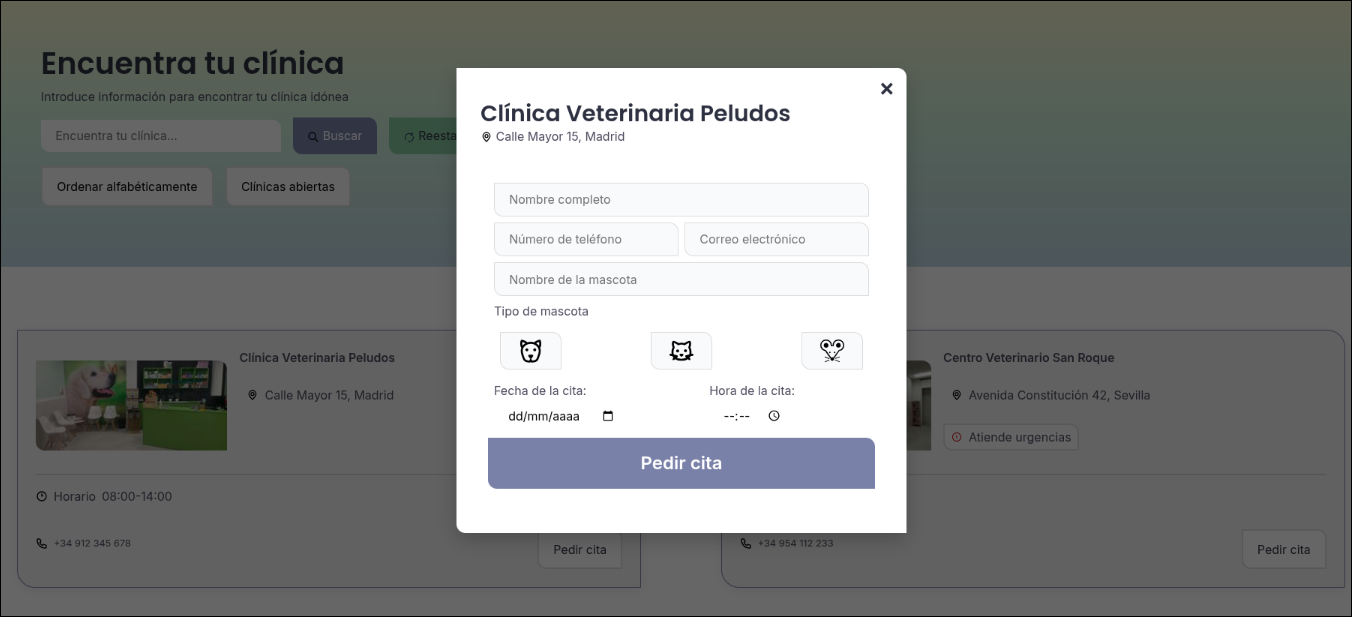
\includegraphics[width=\linewidth,keepaspectratio]{capturas_js/autocompletado-1.png}
        \caption{Formulario previo a la selección}
    \end{minipage}\hfill
    \begin{minipage}{0.48\textwidth}
        \centering
        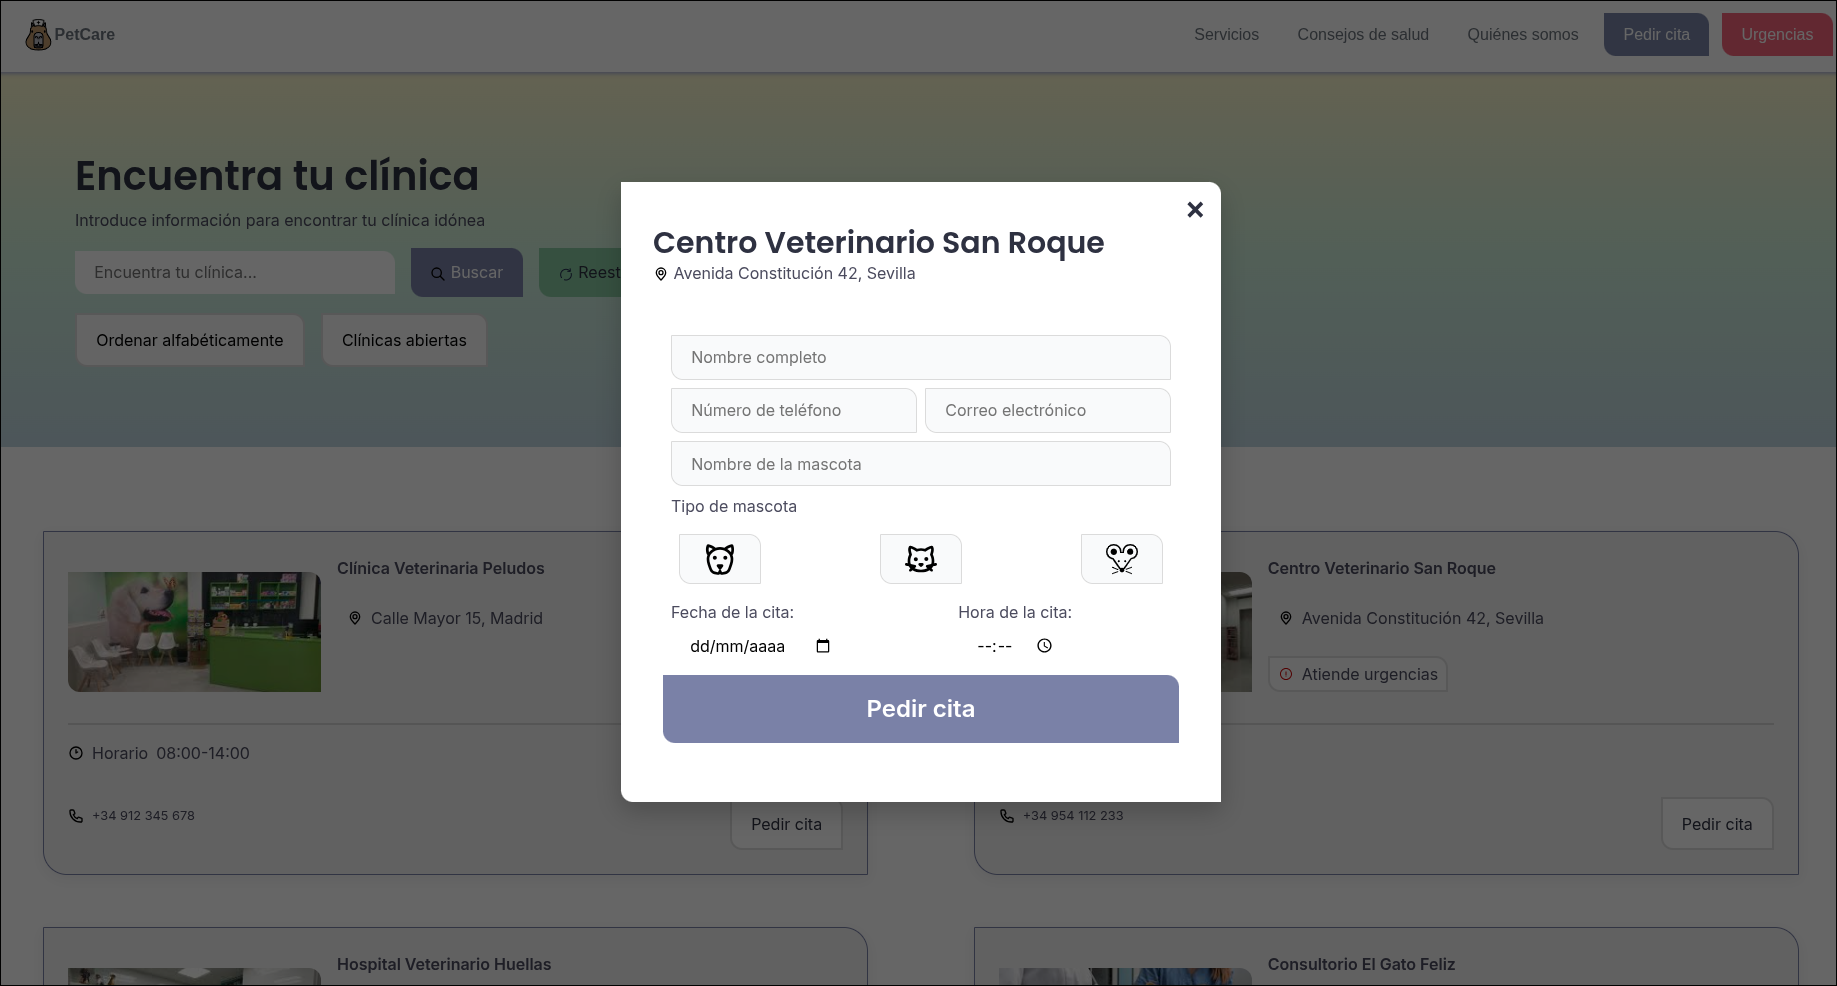
\includegraphics[width=\linewidth,keepaspectratio]{capturas_js/autocompletado-2.png}
        \caption{Formulario autocompletado mediante sessionStorage}
    \end{minipage}
\end{figure}

Para comunicar la página principal con el \textit{iframe}, hemos utilizado la API \texttt{SessionStorage} de HTML5. Las partes críticas del código son:

\begin{itemize}
\item \textbf{Almacenamiento en origen (\texttt{clinicas.js}):} Durante la renderización dinámica de las tarjetas, localizamos el botón de cita mediante \texttt{querySelector(".pedir-cita")} y le asignamos un evento \texttt{click}. Al dispararse el evento, en lugar de modificar el DOM directamente, utilizamos \texttt{sessionStorage.setItem()} para guardar el \texttt{nombre} y la \texttt{ubicacion} de esa clínica específica en la memoria temporal del navegador.
\item \textbf{Recuperación en destino (\texttt{pedir-cita.js}):} El documento \texttt{pedir-cita.html} (que vive dentro del iframe) cuenta con su propio archivo JavaScript. Escuchamos el evento \texttt{DOMContentLoaded} para asegurarnos de que el formulario base ya se ha dibujado.
\item \textbf{Lectura e Inyección en el DOM:} Utilizamos \texttt{sessionStorage.getItem()} para extraer las variables almacenadas previamente. Mediante una comprobación lógica (\texttt{if (nombreclinica)}), validamos que los datos existan. De ser así, localizamos los elementos del DOM correspondientes usando \texttt{querySelector(".titulo")} y \texttt{getElementById('texto-ubicacion-cita')} y actualizamos su texto en pantalla mediante la propiedad \texttt{textContent}.
\item \textbf{Sincronización reactiva (evento \texttt{storage}):} Adicionalmente, el iframe escucha el evento nativo \texttt{storage} de la ventana. Esto garantiza que, si el usuario selecciona una clínica diferente sin cerrar el modal, el formulario se actualiza al instante con los nuevos datos sin necesidad de recargar el iframe.
\end{itemize}

\begin{lstlisting}[language=JavaScript, caption=Guardado de estado en la generación de la tarjeta (clinicas.js)]
// Fragmento dentro del bucle de renderizarTarjetas()
let btncita = copia.querySelector(".pedir-cita");
btncita.addEventListener("click", () => {
	sessionStorage.setItem('nombreclinica', clinica.nombre);
	sessionStorage.setItem('ubicacionclinica', clinica.ubicacion);
});
\end{lstlisting}

\begin{lstlisting}[language=JavaScript, caption=Recuperación e inyección de datos en el iframe modal (pedir-cita.js)]
function actualizarDatosClinica() {
	let nombreclinica    = sessionStorage.getItem('nombreclinica');
	let ubicacionclinica = sessionStorage.getItem('ubicacionclinica');
	if (nombreclinica) {
		document.querySelector(".titulo").textContent = nombreclinica;
	}
	if (ubicacionclinica) {
		document.getElementById('texto-ubicacion-cita').textContent =
			ubicacionclinica;
	}
}

// Se ejecuta al cargar el iframe
document.addEventListener("DOMContentLoaded", function() {
	actualizarDatosClinica();
});

// Escucha cambios en SessionStorage desde la ventana padre
window.addEventListener('storage', function(event) {
	if (event.key === 'nombreclinica' || event.key === 'ubicacionclinica') {
		actualizarDatosClinica();
	}
});
\end{lstlisting}

\clearpage

% ─────────────────────────────────────────────────────────────────────────────
\subsection{Métodos de acceso al DOM}
% ─────────────────────────────────────────────────────────────────────────────

Para manipular los elementos de la página, hemos utilizado los 5 métodos principales que ofrece la API nativa del DOM, seleccionando en cada caso el más eficiente según la necesidad:

\begin{itemize}
\item \texttt{getElementById()}: Utilizado en \texttt{sobre-nosotros.js} para capturar el contenedor único donde se inyecta el texto (\texttt{document.getElementById("area-despliegue-texto")}). Es el método más rápido y directo al apuntar a un ID único.
\item \texttt{querySelector()}: Empleado en \texttt{main.js} para seleccionar el botón del menú móvil a través de su clase (\texttt{document.querySelector('.menu-hamburguesa-moviles')}). Devuelve la primera coincidencia que encuentra.
\item \texttt{querySelectorAll()}: Usado en \texttt{sobre-nosotros.js} para recopilar todos los botones de las pestañas (\texttt{document.querySelectorAll(".btn-pestana")}). Nos devuelve un \texttt{NodeList} que podemos iterar fácilmente.
\item \texttt{getElementsByTagName()}: Utilizado en \texttt{clinicas.js} para localizar la etiqueta oculta de renderizado (\texttt{document.getElementsByTagName("template")[0]}).
\item \texttt{getElementsByClassName()}: Empleado en la función de limpieza de \texttt{clinicas.js} para acceder a las barras de búsqueda (\texttt{document.getElementsByClassName('input-busqueda')}).
\end{itemize}

% ─────────────────────────────────────────────────────────────────────────────
\subsection{Eventos implementados}
% ─────────────────────────────────────────────────────────────────────────────

Para lograr que la página sea interactiva, el código se mantiene ``escuchando'' las acciones del usuario y del propio navegador. Se han implementado múltiples eventos, destacando los tres siguientes por su papel fundamental en la arquitectura de la web:

\begin{enumerate}
\item \texttt{DOMContentLoaded}: Presente en la cabecera de todos los archivos \textit{script} (ej. \texttt{main.js}, \texttt{clinicas.js}). Garantiza que nuestro código JavaScript solo comience a ejecutarse cuando el navegador haya terminado de descargar y construir el árbol DOM, evitando errores por intentar acceder a elementos que aún no existen.
\item \texttt{click}: Utilizado para detectar interacciones directas del usuario con botones o enlaces. Por ejemplo, en \texttt{main.js} para desplegar el menú hamburguesa móvil (\texttt{botonHamburguesa.addEventListener('click', ...)}), o en \texttt{clinicas.js} para los botones de filtrado y ordenación.
\item \texttt{input}: Utilizado en \texttt{clinicas.js} y \texttt{servicios.js} (\texttt{inputBusqueda.addEventListener("input", ...)}). A diferencia de \texttt{keyup} o \texttt{change}, este evento se dispara inmediatamente con cada modificación del texto en la barra de búsqueda (ya sea tecleando, pegando o borrando), permitiéndonos ofrecer un filtrado reactivo en tiempo real.
\end{enumerate}

% ─────────────────────────────────────────────────────────────────────────────
\subsection{Sintaxis ECMAScript 6}
% ─────────────────────────────────────────────────────────────────────────────

Destacan las siguientes implementaciones:

\begin{itemize}
\item \textbf{Funciones Flecha (\textit{Arrow Functions}):} Se han utilizado extensamente en los \textit{callbacks} de eventos y métodos de arrays, eliminando la necesidad de escribir la palabra clave \texttt{function} y manteniendo el contexto de \texttt{this}.
\item \textbf{Variables de bloque (\texttt{let} y \texttt{const}):} Sustituyendo al tradicional \texttt{var} para garantizar que las variables respeten el ámbito de su bloque, previniendo errores de reasignación.
\item \textbf{Async/Await:} En \texttt{servicio-especifico.js} y \texttt{consejos.js}, hemos utilizado esta sintaxis moderna para manejar la asincronía de las peticiones \texttt{fetch}, logrando que el código asíncrono se lea de forma estructurada como si fuera síncrono.
\end{itemize}

\begin{lstlisting}[language=JavaScript, caption=Ejemplo del uso de ES6 con Arrow Functions y Template Literals en servicios.js]
// Arrow function aplicada al iterador forEach
serviciosFiltrados.forEach(servicio => {
	const li = document.createElement("li");
	// Template Literal para la inyeccion dinamica multilineal
	li.innerHTML = `
	<a class="tarjeta-servicio borde-asimetrico-2"
	href="servicio-especifico.html?id=${servicio.id}">
	<img src="${servicio.imagen}" class="borde-asimetrico-2"
	alt="${servicio.nombre}">
	<h3 class="titulo-tarjeta">${servicio.nombre}</h3>
	<p>${servicio.descripcion}</p>
	</a>
	`;
	lista.appendChild(li);
});
\end{lstlisting}

% ─────────────────────────────────────────────────────────────────────────────
\subsection{Uso de objetos jQuery}
% ─────────────────────────────────────────────────────────────────────────────

Aunque gran parte del proyecto se ha desarrollado en JS nativo hemos incorporado la librería \textbf{jQuery} en puntos estratégicos del código, específicamente en las vistas de clínicas y urgencias.

\begin{itemize}
\item \textbf{Selección de nodos y Colecciones:} Hemos utilizado el constructor global \texttt{\$(\ldots)} para capturar elementos de forma concisa. Por ejemplo, en \texttt{clinicas.js}, asignamos a variables objetos de jQuery como \texttt{let contenedor = \$(".contenedor-tarjetas");} o \texttt{let formbusqueda = \$('form[name="buscarClinica"]');}.
\item \textbf{Métodos de manipulación estructural:} Durante el re-renderizado de tarjetas, jQuery nos ahorra escribir bucles de eliminación de nodos hijos gracias a su método \texttt{.empty()}. Una vez generadas las nuevas tarjetas clónicas nativas, las inyectamos fácilmente usando \texttt{contenedor.append(copia)}.
\item \textbf{Lectura rápida de valores:} En el buscador, extraer y sanitizar el texto del input se reduce a una sola línea gracias al método \texttt{.val()} concatenado con funciones de cadena nativas: \texttt{\$('.input-busqueda').val().toLowerCase().trim()}.
\item \textbf{Asignación de eventos:} En lugar del verboso \texttt{addEventListener}, el objeto jQuery de nuestro formulario delega los eventos de teclado de forma compacta mediante el método \texttt{.on()}: \texttt{formbusqueda.on('input', funcbusqueda);}.
\end{itemize}

\begin{lstlisting}[language=JavaScript, caption=Manipulación del DOM y eventos mediante jQuery en clinicas.js]
function inicializarBuscador() {
	// 1. Creacion de un objeto jQuery desde un selector CSS
	let formbusqueda = $('form[name="buscarClinica"]');
	
	let funcbusqueda = (e) => {
		e.preventDefault();
		// 2. Uso del metodo .val() propio de jQuery
		let txt = $('.input-busqueda').val().toLowerCase().trim();
		let clinicasFiltradas = clinicasGlobal.filter(clinica =>
		clinica.nombre.toLowerCase().includes(txt)
		);
		renderizarTarjetas(clinicasFiltradas);
	};
	
	// 3. Asignacion de eventos con el metodo .on()
	formbusqueda.on('submit', funcbusqueda);
	formbusqueda.on('input', funcbusqueda);
}
\end{lstlisting}

\clearpage

% ─────────────────────────────────────────────────────────────────────────────
\subsection{Carga de contenido en formato XML}
% ─────────────────────────────────────────────────────────────────────────────

Para la sección de ``Servicios'', la información detallada de cada especialidad veterinaria se ha estructurado y almacenado en un archivo externo en formato XML (\texttt{servicios.xml}).

A continuación, se muestra un extracto simplificado de la estructura del archivo XML, donde cada especialidad está encapsulada en una etiqueta \texttt{<servicio>} provista de un atributo \texttt{id} único, conteniendo a su vez etiquetas descriptivas y múltiples bloques de texto:

\begin{lstlisting}[language=XML, caption=Estructura del archivo de datos servicios.xml]
<?xml version="1.0" encoding="UTF-8"?>
<servicios>
<servicio id="neurologia">
<nombre>Neurologia</nombre>
<imagen>assets/imgs/servicios-neurologia.png</imagen>
<descripcion-corta>Evaluacion y tratamiento de trastornos...</descripcion-corta>
<subtitulo>Expertos en el cuidado del sistema nervioso</subtitulo>
<bloque>
<titulo>1. Evaluacion Neurologica Completa</titulo>
<texto>Realizamos examenes exhaustivos de los reflejos...</texto>
</bloque>
</servicio>
</servicios>
\end{lstlisting}

\subsubsection{Método utilizado: Objeto \texttt{XMLHttpRequest}}

Para cumplir con la exigencia de implementar diversas formas de carga asíncrona de datos, en la página general de Servicios hemos consumido este archivo XML utilizando el objeto nativo \textbf{\texttt{XMLHttpRequest}}.

La implementación sigue un flujo basado en eventos y comprobaciones de estado:

\begin{itemize}
\item \textbf{Instanciación y Configuración:} Creamos una nueva instancia mediante \texttt{new XMLHttpRequest()} y configuramos la petición con el método \texttt{.open("GET", "assets/xml/servicios.xml", true)}, indicando que es una petición asíncrona (\texttt{true}).
\item \textbf{Escucha de cambios de estado:} Asignamos una función al controlador de eventos \texttt{.onreadystatechange}. El navegador invocará esta función en cada fase del ciclo de vida de la petición.
\item \textbf{Validación:} Dentro del evento, comprobamos de forma estricta que \texttt{xhr.readyState === 4} (operación de red completada) y que \texttt{xhr.status === 200} (código de éxito HTTP).
\item \textbf{Parseo automático:} Una de las grandes ventajas de \texttt{XMLHttpRequest} al trabajar con XML es su propiedad \texttt{.responseXML}. Si el documento XML está bien formado, el navegador lo convierte automáticamente en un árbol de nodos manipulable.
\end{itemize}

\begin{lstlisting}[language=JavaScript, caption=Carga asíncrona y parseo de XML mediante XMLHttpRequest en servicios.js]
function cargarServicios() {
	let xhr = new XMLHttpRequest();
	xhr.open("GET", "assets/xml/servicios.xml", true);
	xhr.onreadystatechange = function () {
		if (xhr.readyState === 4 && xhr.status === 200) {
			let documentoXML = xhr.responseXML;
			procesarServicios(documentoXML);
		}
	};
	xhr.onerror = function() {
		console.error("Error al cargar servicios:", xhr.statusText);
	};
	xhr.send();
}

function procesarServicios(xmlDoc) {
	let listaServicios = xmlDoc.getElementsByTagName("servicio");
	Array.from(listaServicios).forEach(servicio => {
		let id     = servicio.getAttribute("id");
		let nombre = servicio.getElementsByTagName("nombre")[0]
		.textContent.trim();
		// ... almacenamiento y renderizado omitidos
	});
}
\end{lstlisting}

\textit{Nota metodológica:} Para la página de detalle de un servicio individual (\texttt{servicio-especifico.js}), hemos utilizado una tercera aproximación técnica: la moderna \textbf{API Fetch} combinada con la clase \textbf{\texttt{DOMParser}} para transformar la respuesta de texto en un documento XML.

\begin{figure}[H]
\centering
\rotatebox{90}{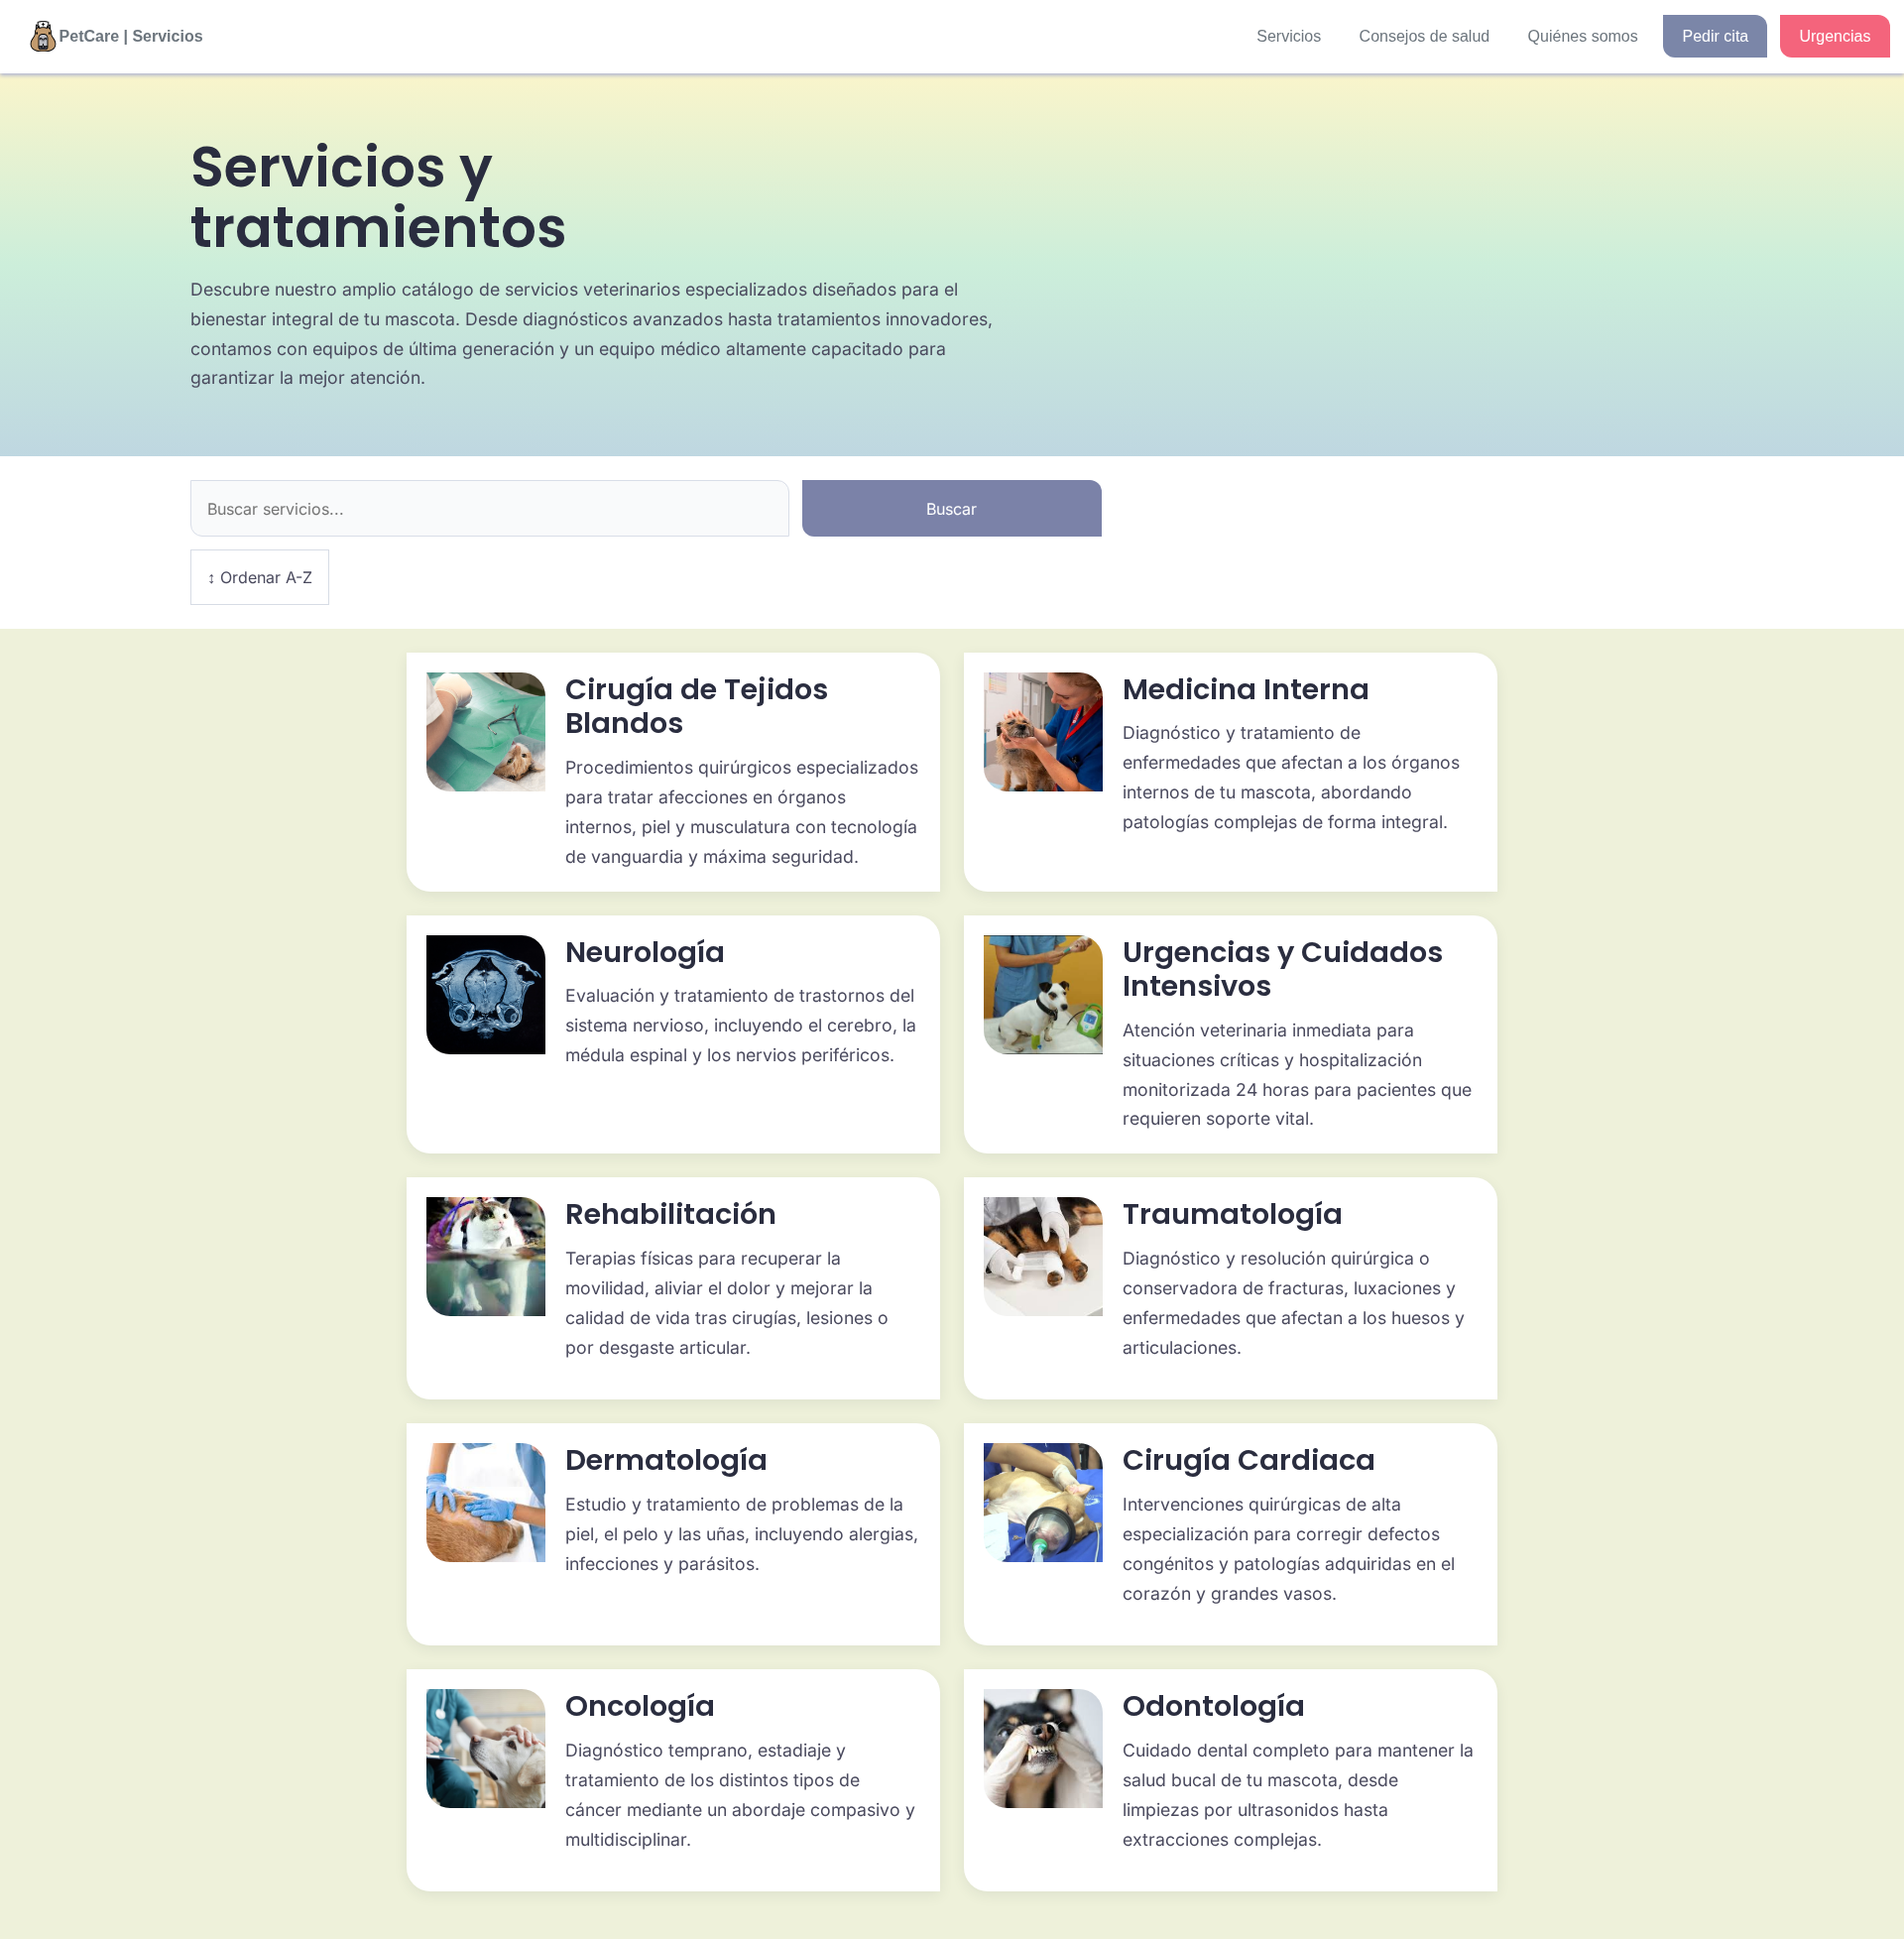
\includegraphics[width=0.85\textheight,keepaspectratio]{capturas_responsivas/servicios-desktop.png}}
\caption{Servicios: carga dinámica desde XML en escritorio}
\end{figure}

\begin{figure}[H]
\centering
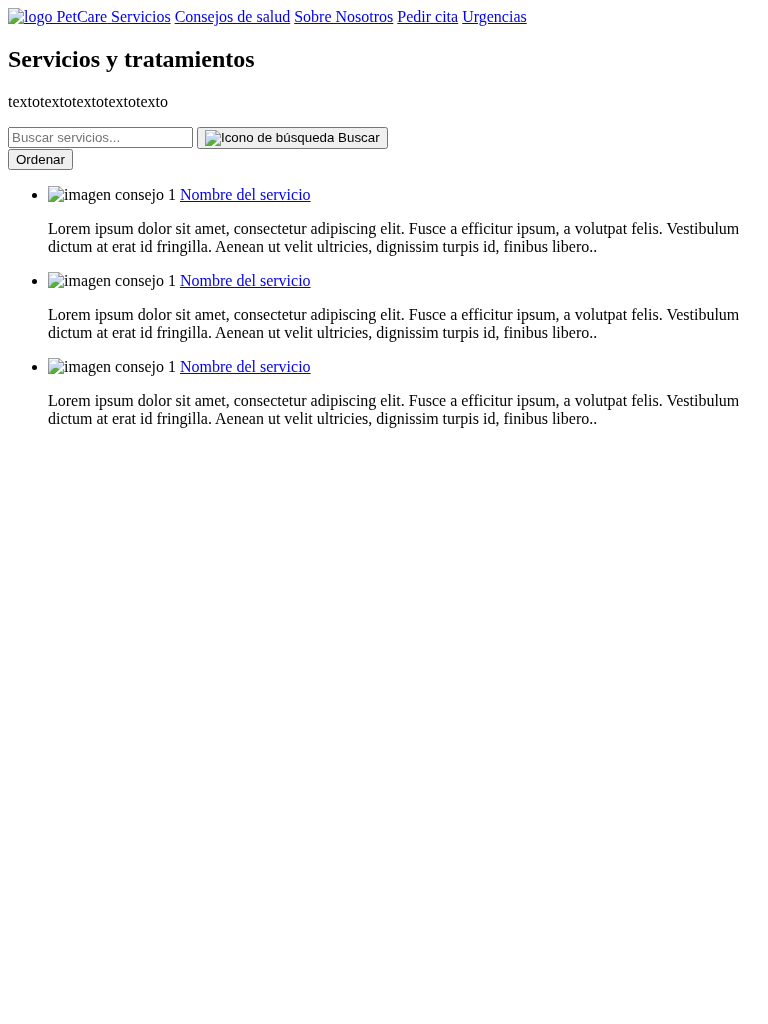
\includegraphics[width=0.65\linewidth,height=0.55\textheight,keepaspectratio]{capturas_responsivas/servicios-tablet.png}
\caption{Servicios: carga dinámica desde XML en tablet}
\end{figure}

\begin{figure}[H]
\centering
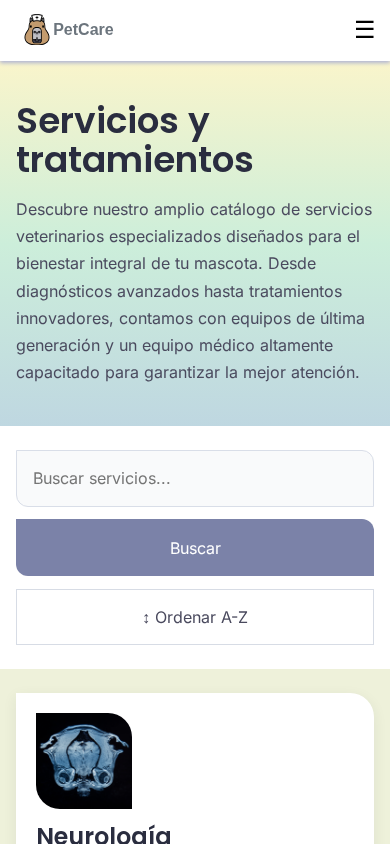
\includegraphics[width=0.38\linewidth,height=0.55\textheight,keepaspectratio]{capturas_responsivas/servicios-mobile.png}
\caption{Servicios: carga dinámica desde XML en móvil}
\end{figure}

\clearpage

% ─────────────────────────────────────────────────────────────────────────────
\subsection{Carga de contenido en formato JSON}
% ─────────────────────────────────────────────────────────────────────────────

Para dotar al sitio web de información dinámica y fácilmente actualizable, los datos estructurados de los centros veterinarios se han externalizado en un archivo local llamado \texttt{clinicas.json}. Este archivo actúa como una base de datos de solo lectura que alimenta tanto a la página de ``Clínicas'' como a la de ``Urgencias''.

A continuación, se muestra un fragmento representativo de la estructura de este archivo JSON:

\begin{lstlisting}[language=json, caption=Estructura simplificada del archivo clinicas.json]
{
	"clinicas": [
	{
		"nombre": "Clinica Veterinaria Peludos",
		"ubicacion": "Calle Mayor 15, Madrid",
		"foto": "assets/imgs/clinica-1.jpeg",
		"horario": "08:00-14:00",
		"telefono": "+34 912 345 678",
		"urgencias": false
	},
	{
		"nombre": "Centro Veterinario San Roque",
		"ubicacion": "Avenida Constitucion 42, Sevilla",
		"foto": "assets/imgs/clinica-2.jpeg",
		"horario": "10:00-21:30",
		"telefono": "+34 954 112 233",
		"urgencias": true
	}
	]
}
\end{lstlisting}

\subsubsection{Método utilizado: objeto jQuery (\texttt{\$.getJSON})}

El enunciado de la práctica requiere utilizar distintas formas para la carga de datos. Para el caso específico de las clínicas y urgencias, hemos optado por utilizar la librería \textbf{jQuery}, concretamente su método asíncrono \texttt{\$.getJSON()}.

Este método realiza la petición HTTP y, de forma automática, parsea la cadena de texto JSON transformándola en un objeto nativo de JavaScript listo para ser iterado, ahorrándonos el paso de usar \texttt{JSON.parse()}.

\begin{lstlisting}[language=JavaScript, caption=Carga asíncrona de JSON mediante jQuery en clinicas.js]
let clinicasGlobal = [];
document.addEventListener("DOMContentLoaded", function() {
	$.getJSON("assets/json/clinicas.json", (datos) => {
		clinicasGlobal = datos.clinicas;

		// Lee el termino procedente del buscador de la portada
		const urlParams = new URLSearchParams(window.location.search);
		const busqueda = urlParams.get('clinica');

		if (busqueda) {
			const clinicasFiltradas = clinicasGlobal.filter(c =>
				c.nombre.toLowerCase().includes(busqueda.toLowerCase())
			);
			renderizarTarjetas(clinicasFiltradas);
			$('.input-busqueda').val(busqueda);
		} else {
			renderizarTarjetas(clinicasGlobal);
		}

		inicializarBuscador();
		inicializarOrden();
		inicializarHorario();
	});
});
\end{lstlisting}

\textbf{Implementación en la página de Urgencias}

En el archivo \texttt{urgencias.js}, reutilizamos el mismo archivo \texttt{clinicas.json} mediante \texttt{\$.getJSON()}, pero aplicamos una lógica de negocio diferente en el \textit{callback}. En lugar de mostrar todas las clínicas, iteramos sobre los datos recibidos utilizando el método \texttt{.filter()} para extraer únicamente aquellas que cumplan dos condiciones simultáneas:

\begin{enumerate}
\item Que su atributo \texttt{urgencias} sea \texttt{true}.
\item Que la hora actual del sistema del usuario esté dentro del rango definido en su atributo \texttt{horario}.
\end{enumerate}

\begin{lstlisting}[language=JavaScript, caption=Filtrado en tiempo de ejecución tras la carga del JSON en urgencias.js]
document.addEventListener("DOMContentLoaded", function () {
	$.getJSON("assets/json/clinicas.json", (datos) => {
		const clinicas = datos.clinicas;
		const ahora = new Date();
		const minutosActuales = (ahora.getHours() * 60) + ahora.getMinutes();
		
		const clinicasDisponibles = clinicas.filter((clinica) => {
			return clinica.urgencias &&
			estaDisponibleAhora(clinica.horario, minutosActuales);
		});
		
		clinicasDisponibles.forEach((clinica) => {
			// (Logica de clonacion del template omitida)
		});
	});
});
\end{lstlisting}

\begin{figure}[H]
\centering
\rotatebox{90}{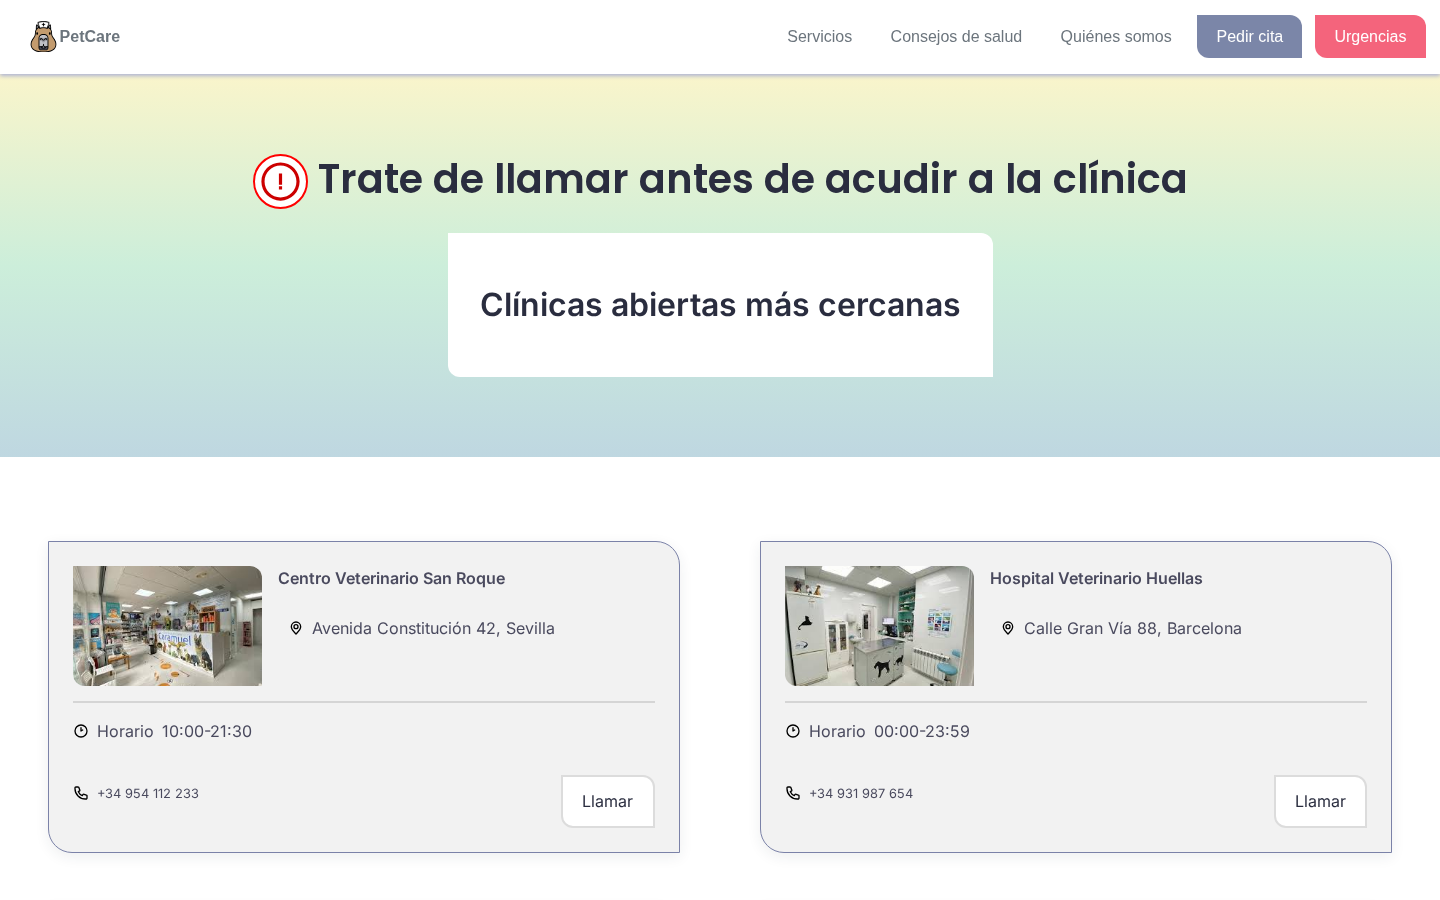
\includegraphics[width=0.85\textheight,keepaspectratio]{capturas_responsivas/urgencias-desktop.png}}
\caption{Urgencias: clínicas filtradas dinámicamente desde JSON en escritorio}
\end{figure}

\begin{figure}[H]
\centering
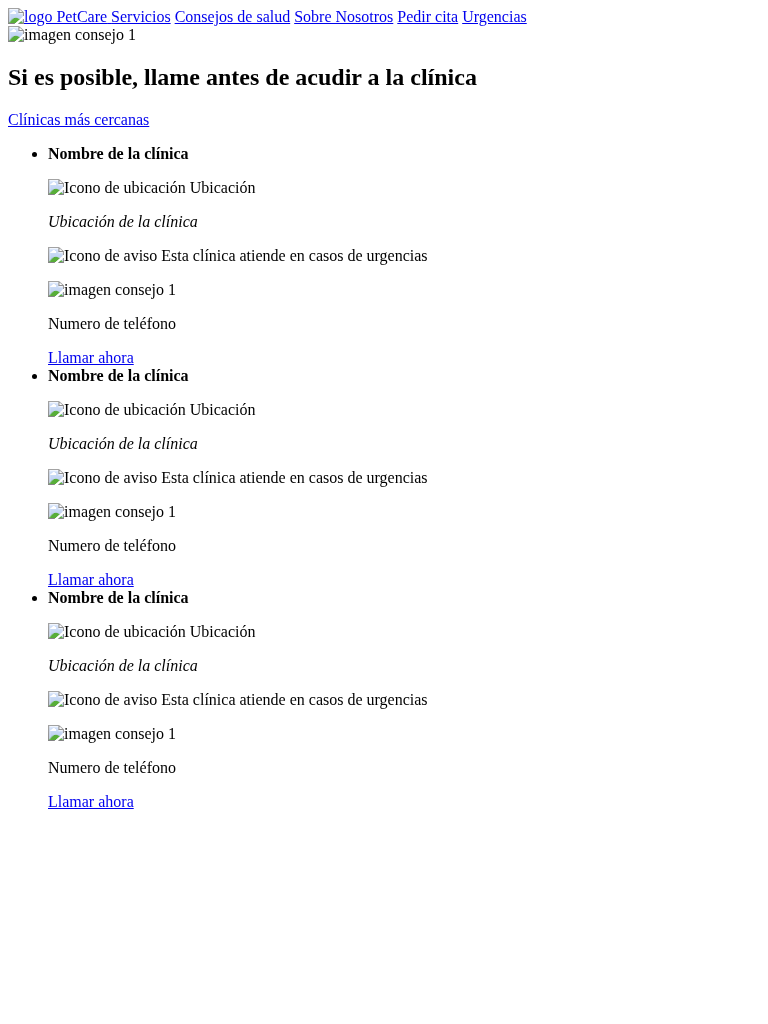
\includegraphics[width=0.65\linewidth,height=0.55\textheight,keepaspectratio]{capturas_responsivas/urgencias-tablet.png}
\caption{Urgencias: clínicas filtradas dinámicamente desde JSON en tablet}
\end{figure}

\begin{figure}[H]
\centering
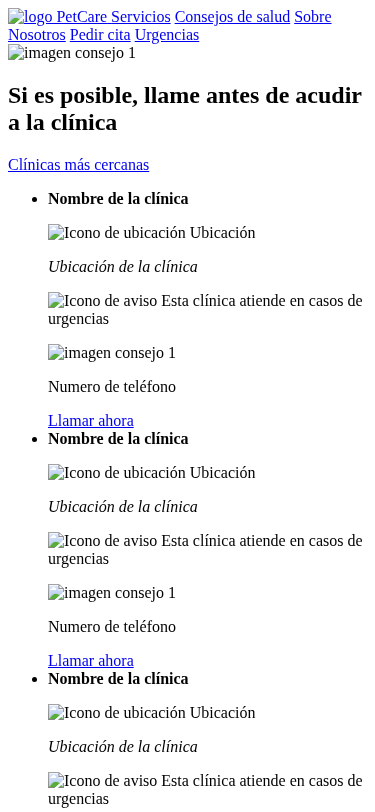
\includegraphics[width=0.38\linewidth,height=0.55\textheight,keepaspectratio]{capturas_responsivas/urgencias-mobile.png}
\caption{Urgencias: clínicas filtradas dinámicamente desde JSON en móvil}
\end{figure}

\clearpage
\appendix

% =============================================================================
\section{Galería las versiones finales de las páginas}
% =============================================================================

Este apéndice recoge capturas de pantalla de la versión final de cada página del sitio en los tres formatos de visualización: escritorio (1440\,px), tablet (768\,px) y móvil (390\,px), mostrando el comportamiento responsivo del conjunto completo de la interfaz.

% ─────────────────────────────────────────────────────────────────────────────
\subsection{Página principal}
% ─────────────────────────────────────────────────────────────────────────────

\begin{figure}[H]
\centering
\rotatebox{90}{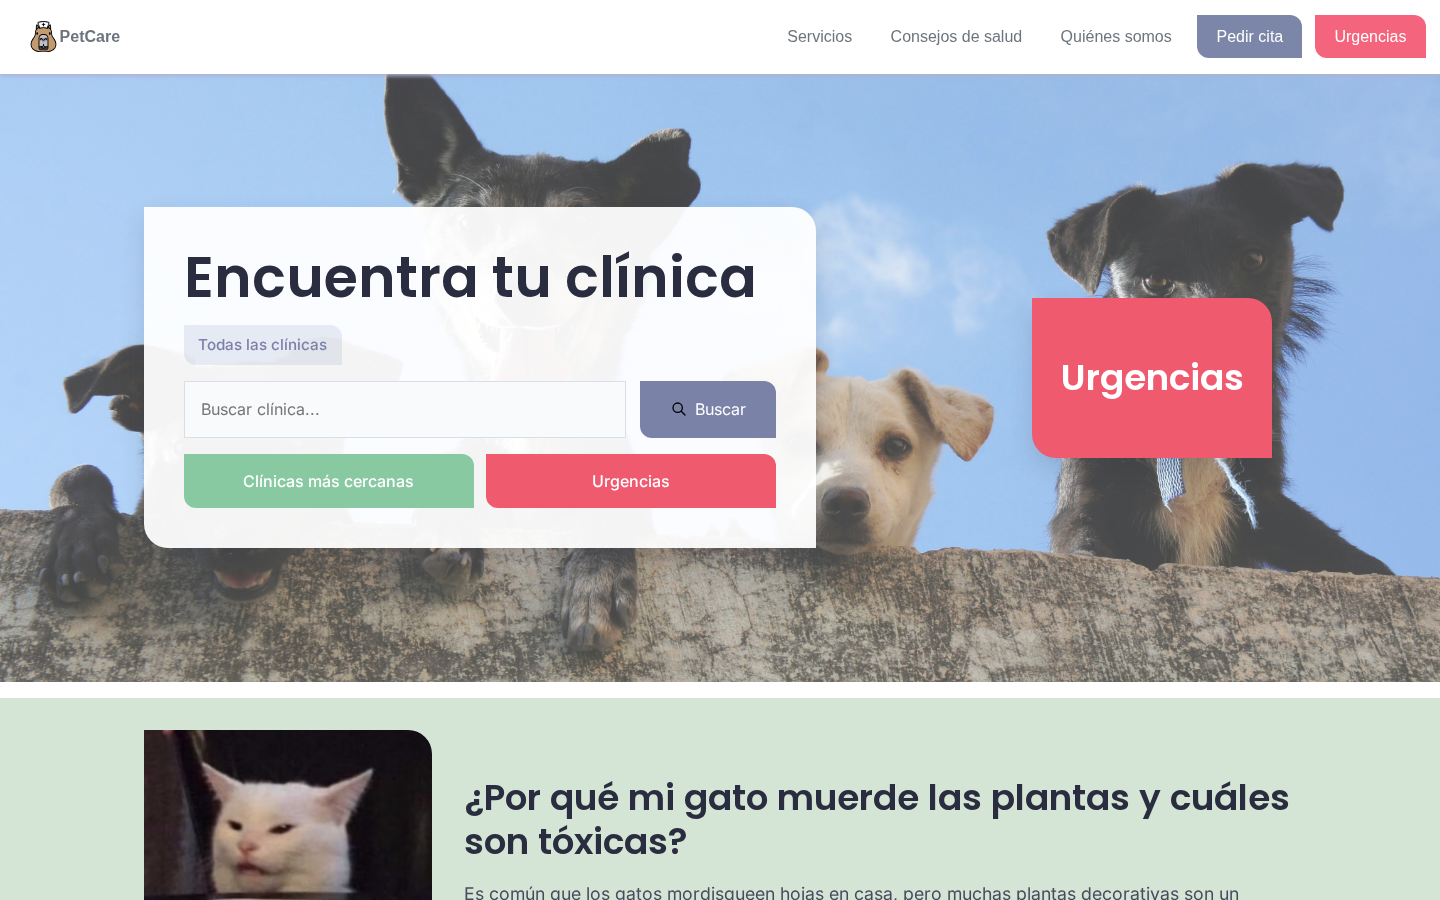
\includegraphics[width=0.85\textheight,keepaspectratio]{capturas_responsivas/index-desktop.png}}
\caption{Página principal --- escritorio}
\end{figure}

\begin{figure}[H]
\centering
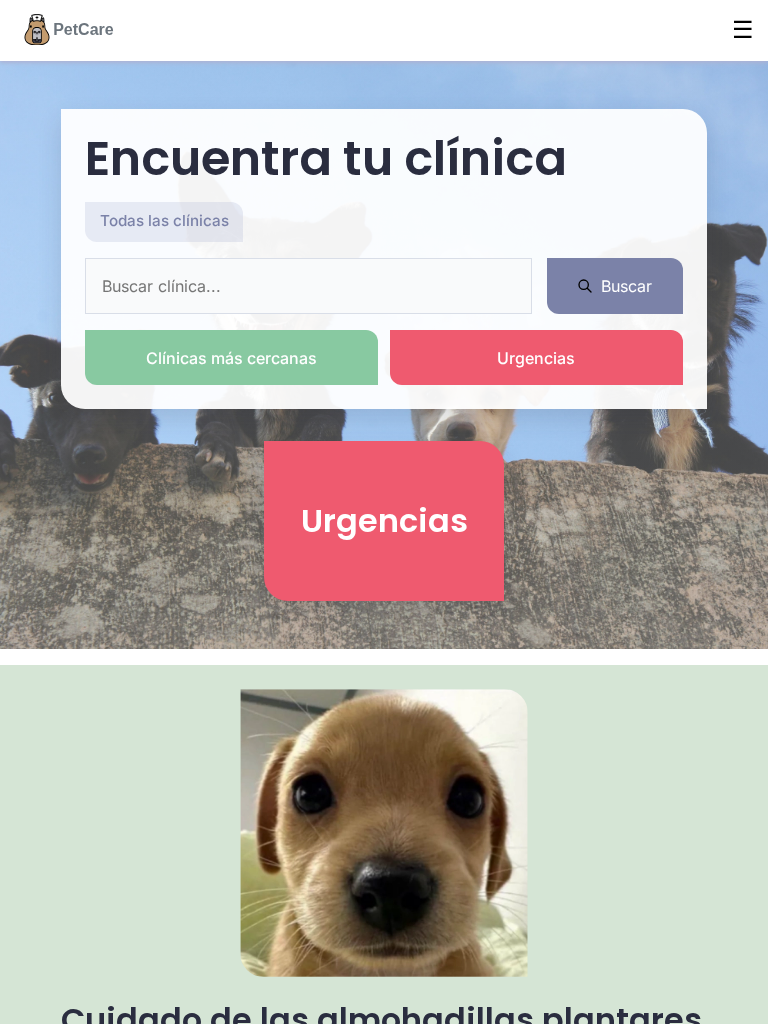
\includegraphics[width=0.70\linewidth,height=0.65\textheight,keepaspectratio]{capturas_responsivas/index-tablet.png}
\caption{Página principal --- tablet}
\end{figure}

\begin{figure}[H]
\centering
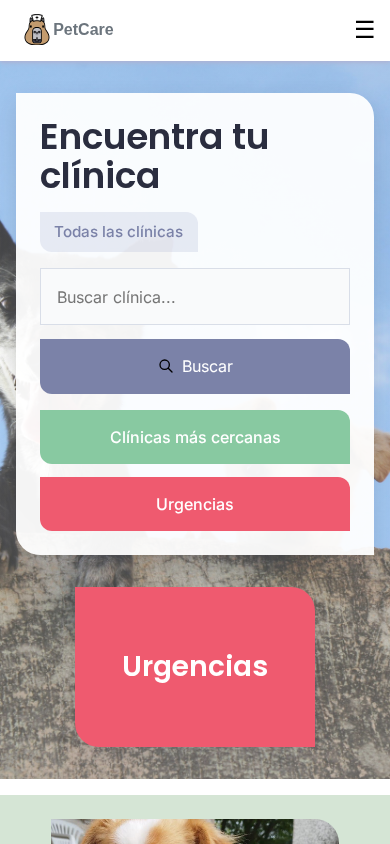
\includegraphics[width=0.38\linewidth,height=0.65\textheight,keepaspectratio]{capturas_responsivas/index-mobile.png}
\caption{Página principal --- móvil}
\end{figure}

\clearpage

% ─────────────────────────────────────────────────────────────────────────────
\subsection{Clínicas}
% ─────────────────────────────────────────────────────────────────────────────

\begin{figure}[H]
\centering
\rotatebox{90}{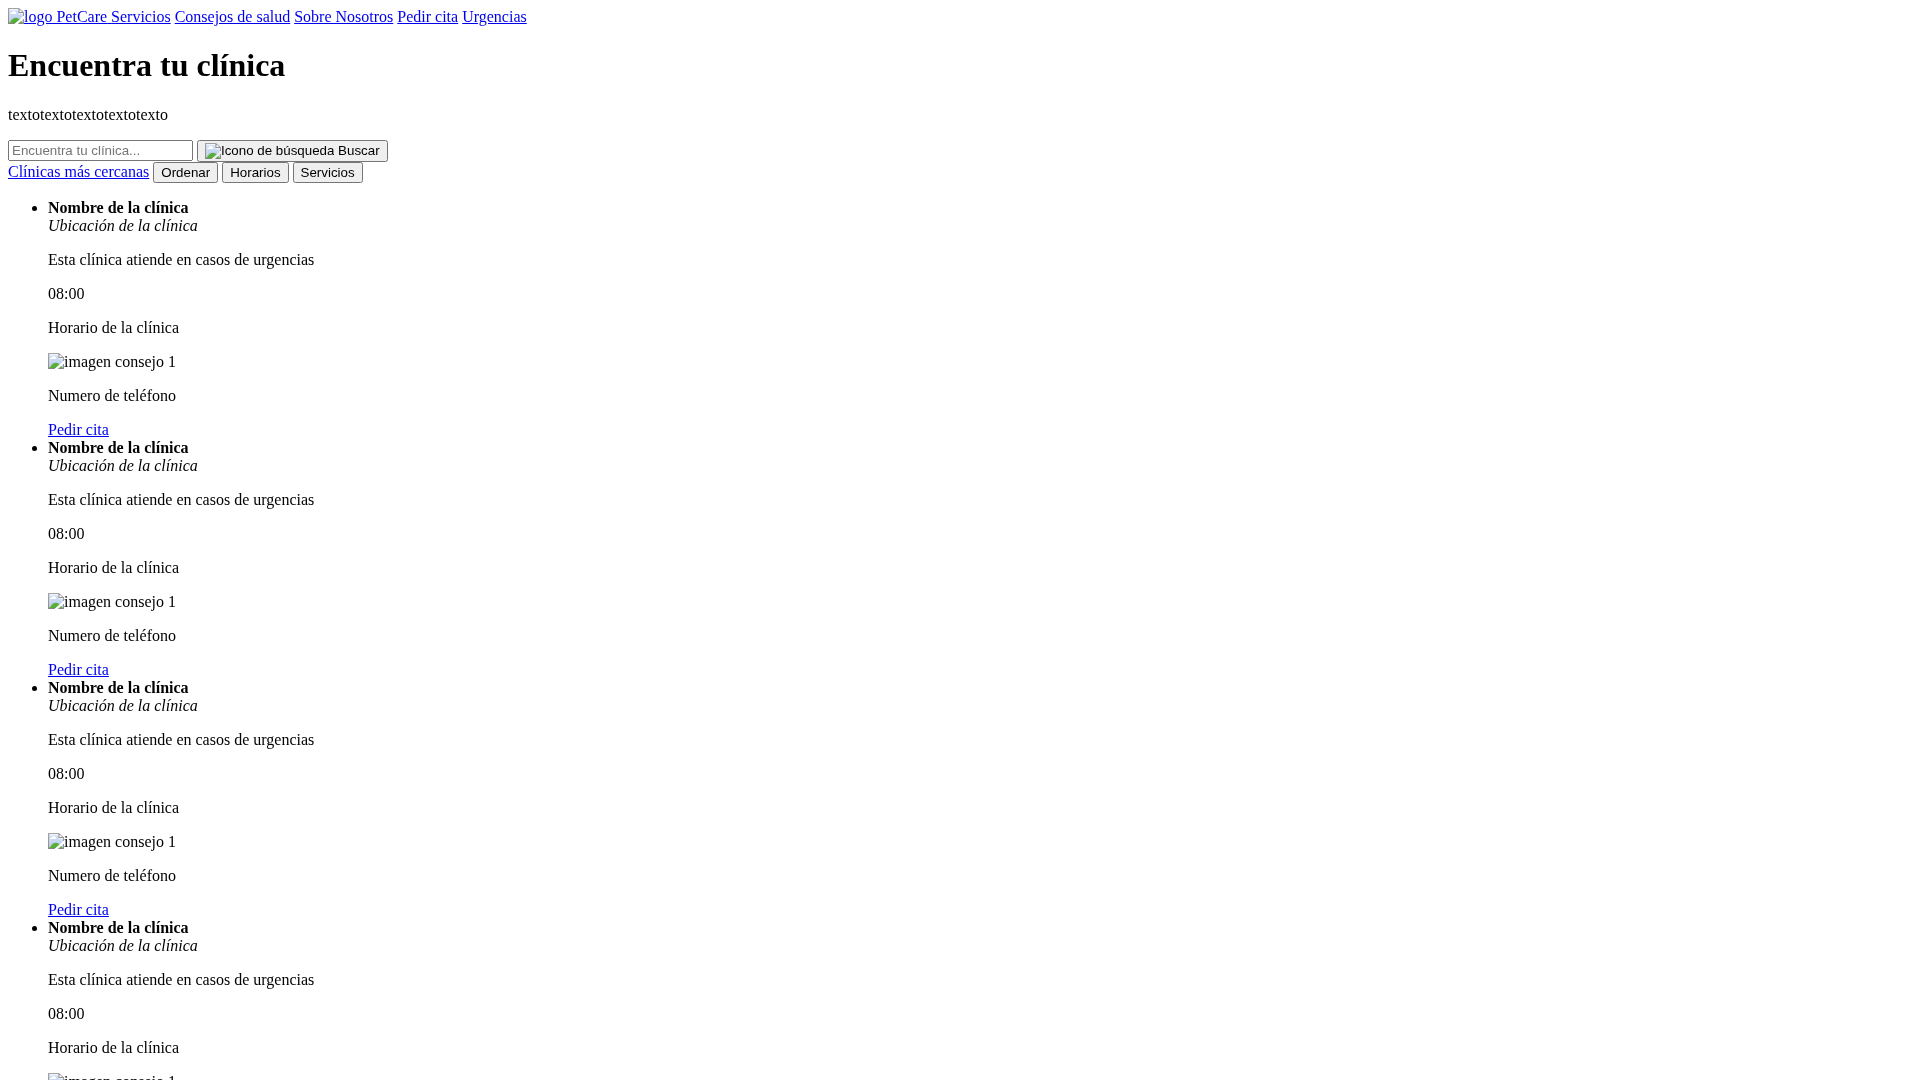
\includegraphics[width=0.85\textheight,keepaspectratio]{capturas_responsivas/clinicas-desktop.png}}
\caption{Clínicas --- escritorio}
\end{figure}

\begin{figure}[H]
\centering
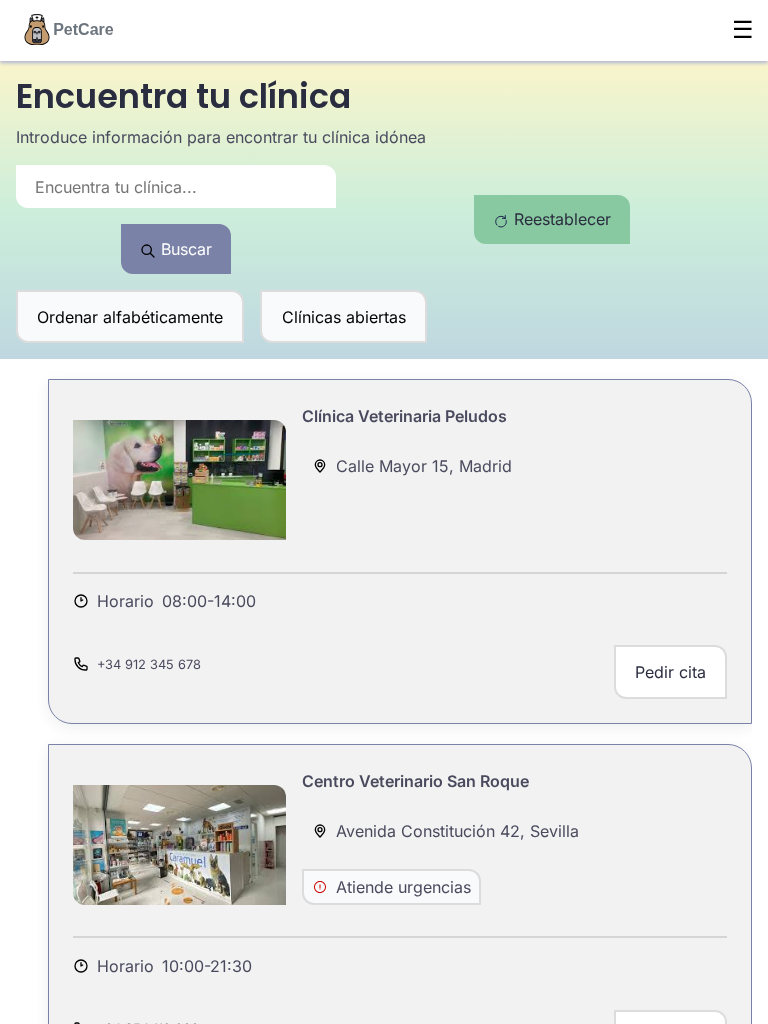
\includegraphics[width=0.70\linewidth,height=0.65\textheight,keepaspectratio]{capturas_responsivas/clinicas-tablet.png}
\caption{Clínicas --- tablet}
\end{figure}

\begin{figure}[H]
\centering
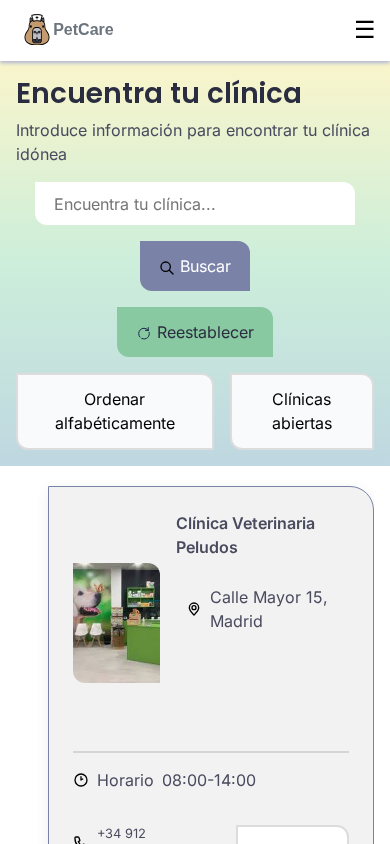
\includegraphics[width=0.38\linewidth,height=0.65\textheight,keepaspectratio]{capturas_responsivas/clinicas-mobile.png}
\caption{Clínicas --- móvil}
\end{figure}

\clearpage

% ─────────────────────────────────────────────────────────────────────────────
\subsection{Urgencias}
% ─────────────────────────────────────────────────────────────────────────────

\begin{figure}[H]
\centering
\rotatebox{90}{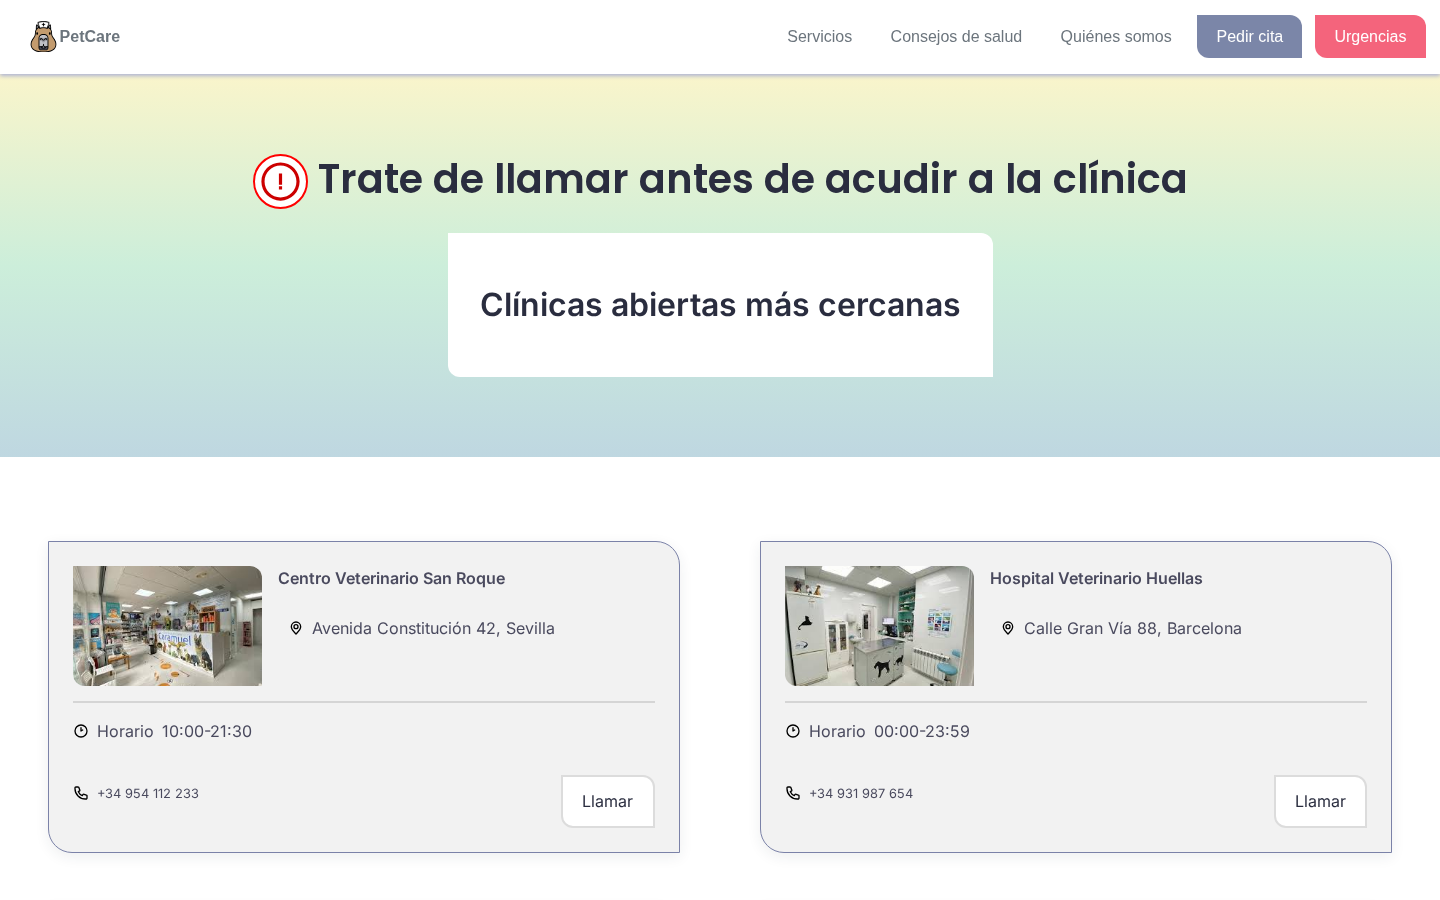
\includegraphics[width=0.85\textheight,keepaspectratio]{capturas_responsivas/urgencias-desktop.png}}
\caption{Urgencias --- escritorio}
\end{figure}

\begin{figure}[H]
\centering
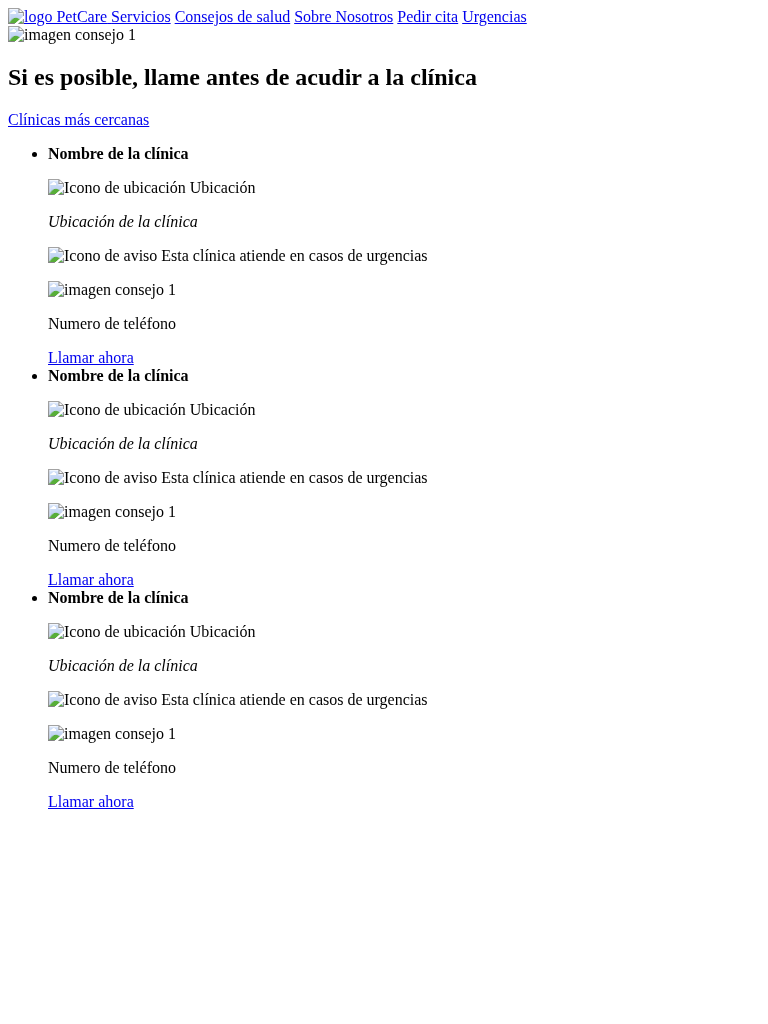
\includegraphics[width=0.70\linewidth,height=0.65\textheight,keepaspectratio]{capturas_responsivas/urgencias-tablet.png}
\caption{Urgencias --- tablet}
\end{figure}

\begin{figure}[H]
\centering
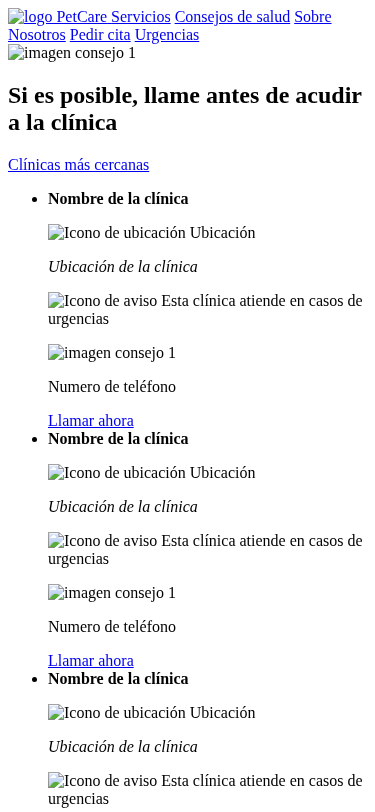
\includegraphics[width=0.38\linewidth,height=0.65\textheight,keepaspectratio]{capturas_responsivas/urgencias-mobile.png}
\caption{Urgencias --- móvil}
\end{figure}

\clearpage

% ─────────────────────────────────────────────────────────────────────────────
\subsection{Servicios}
% ─────────────────────────────────────────────────────────────────────────────

\begin{figure}[H]
\centering
\rotatebox{90}{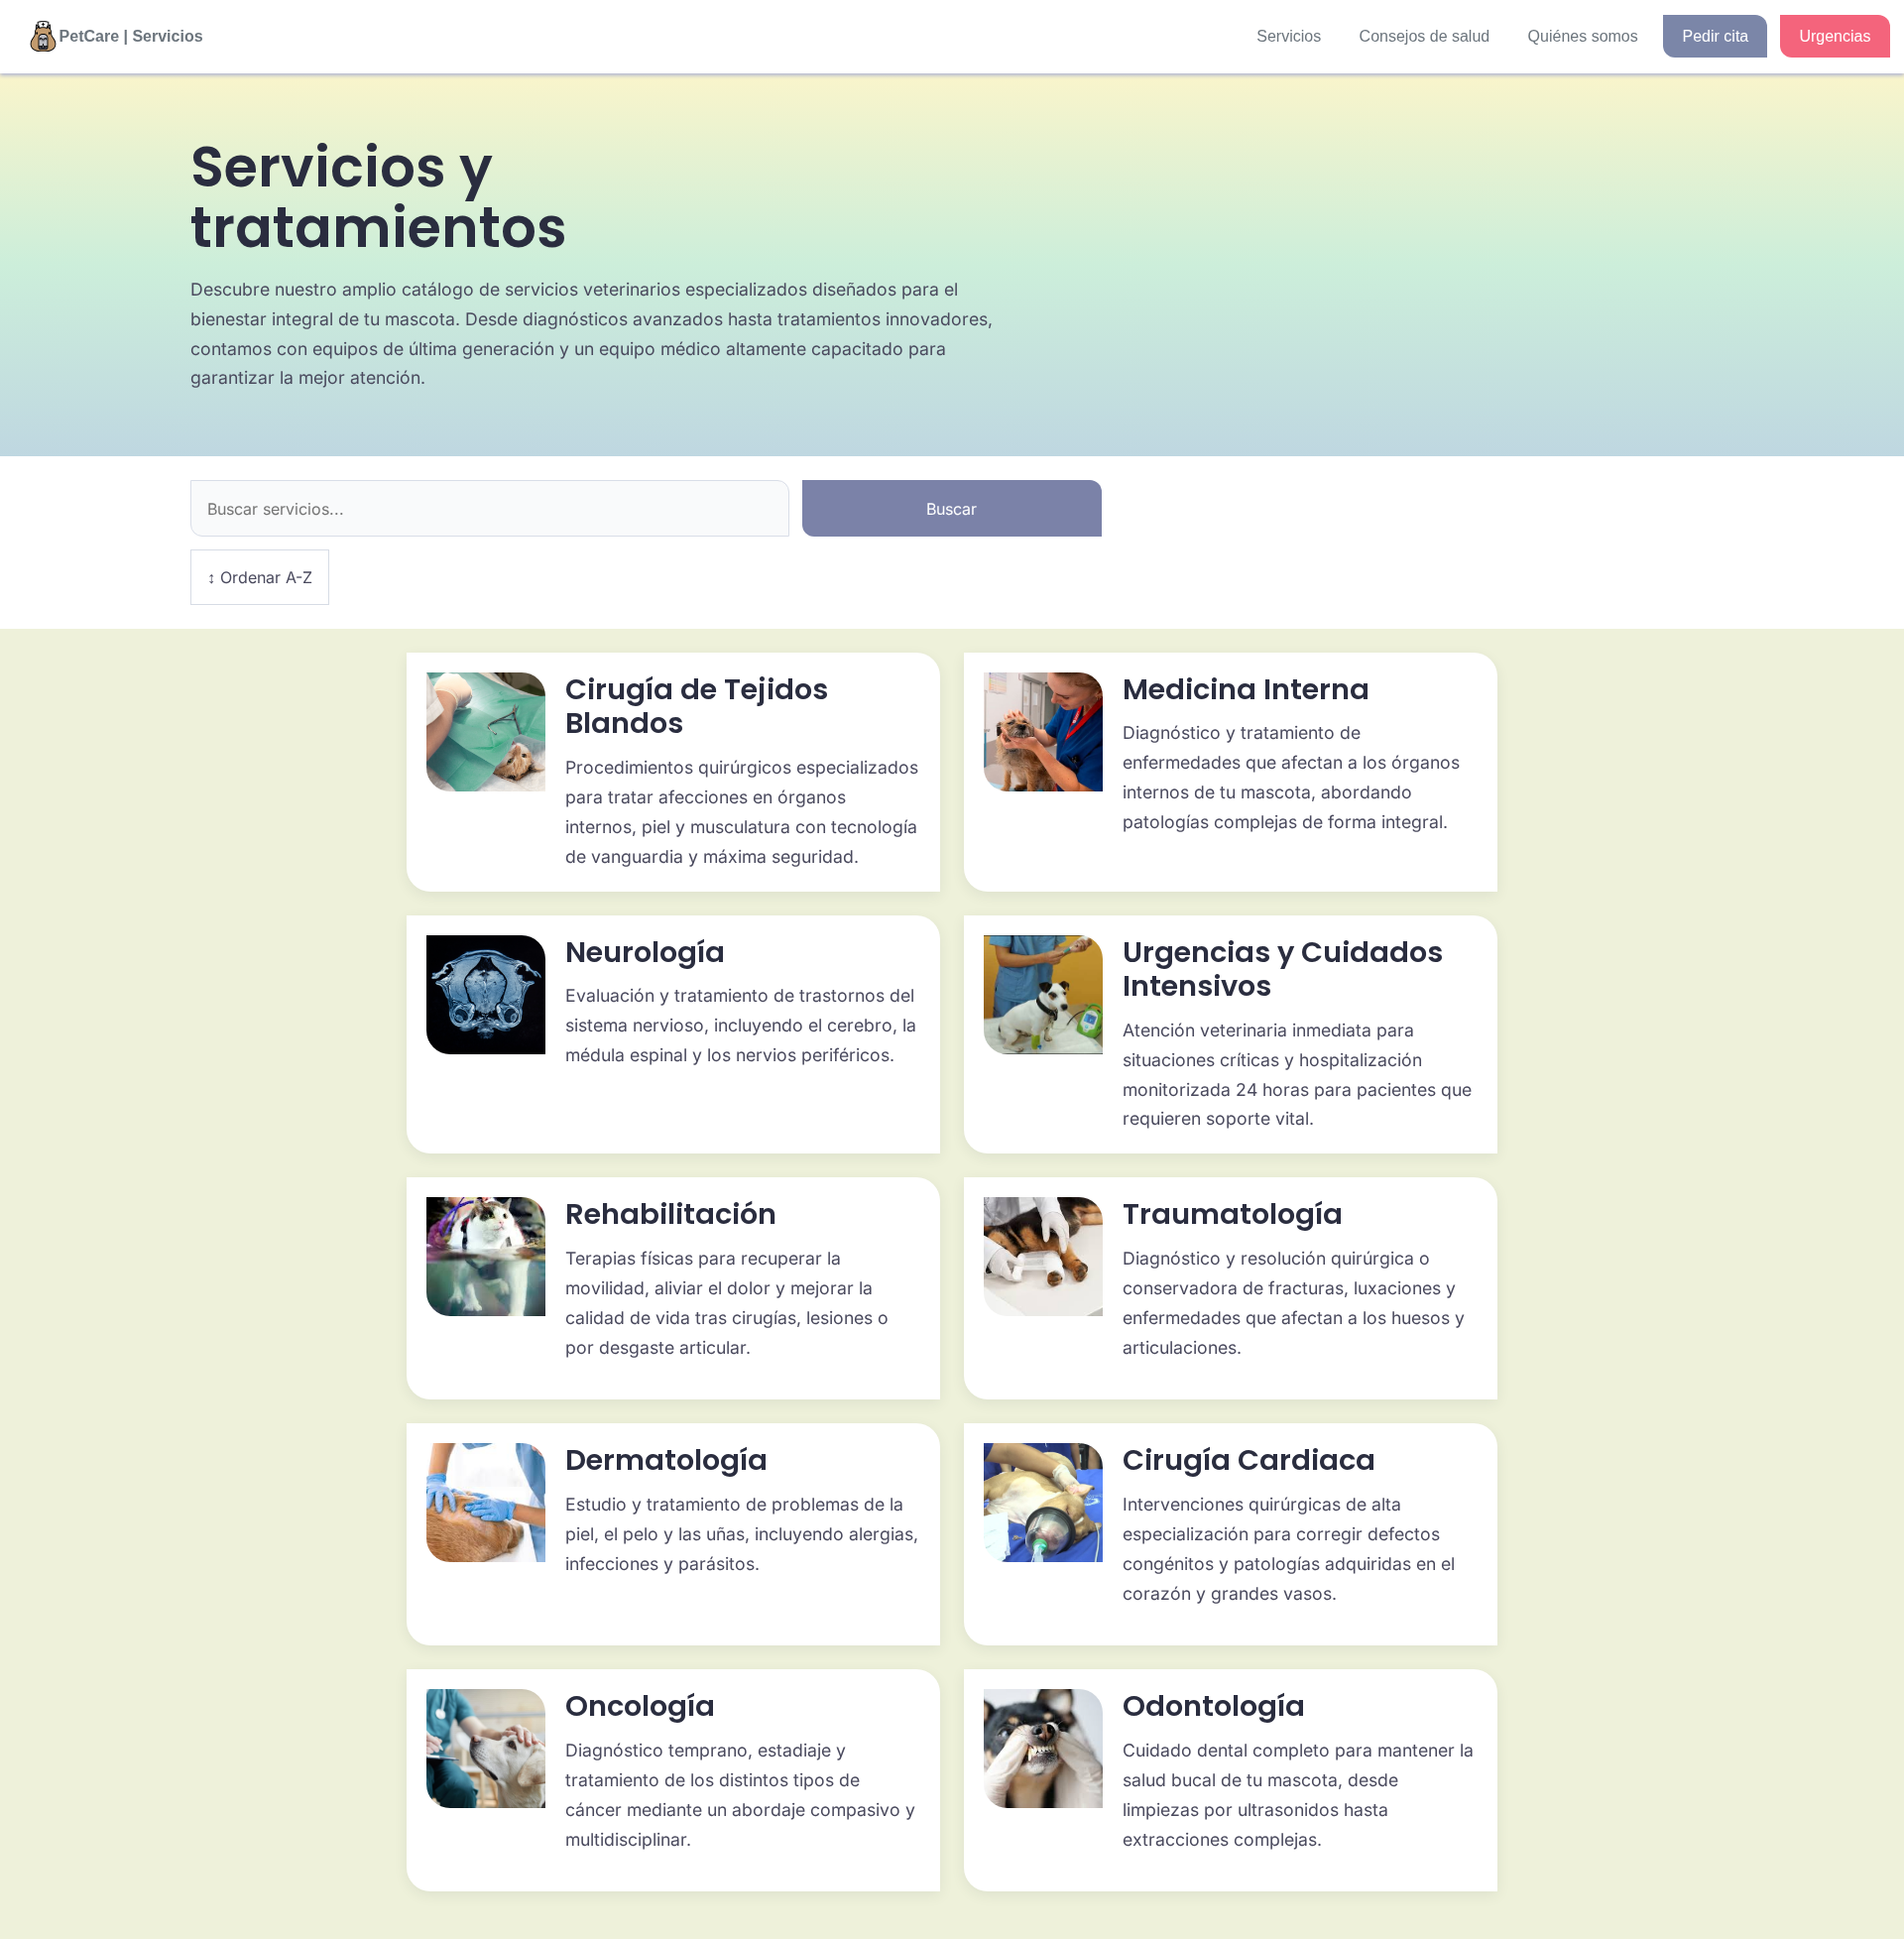
\includegraphics[width=0.85\textheight,keepaspectratio]{capturas_responsivas/servicios-desktop.png}}
\caption{Servicios --- escritorio}
\end{figure}

\begin{figure}[H]
\centering
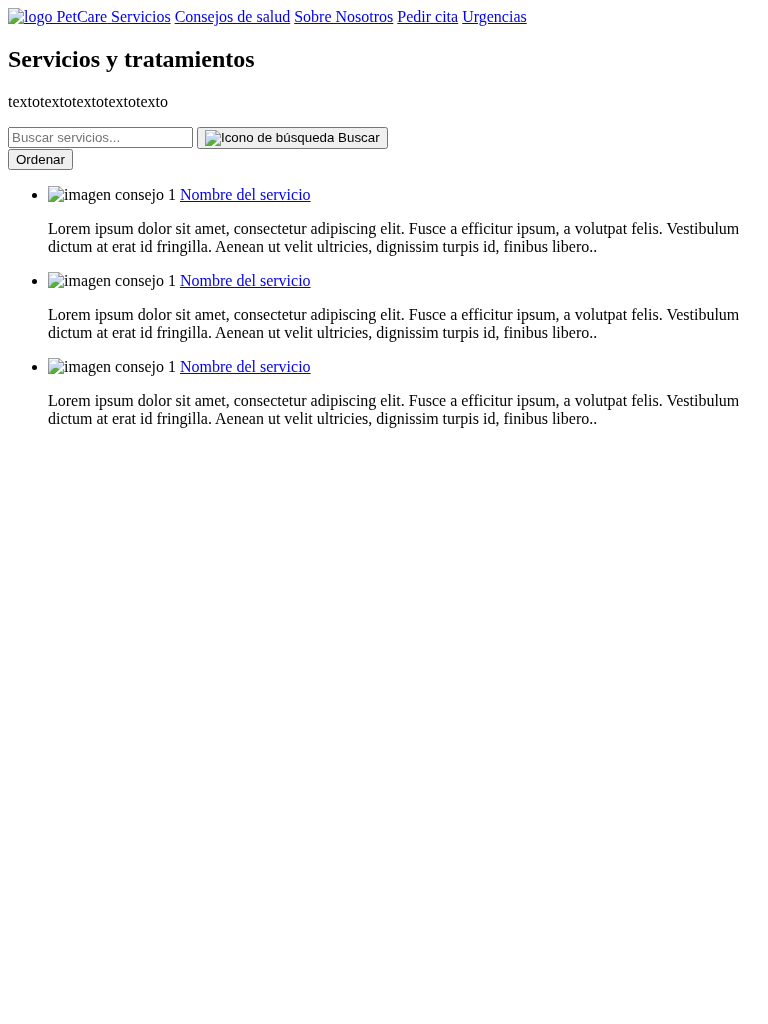
\includegraphics[width=0.70\linewidth,height=0.65\textheight,keepaspectratio]{capturas_responsivas/servicios-tablet.png}
\caption{Servicios --- tablet}
\end{figure}

\begin{figure}[H]
\centering
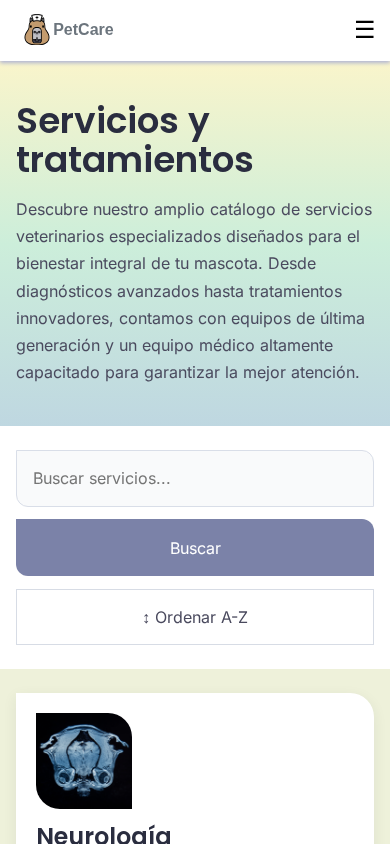
\includegraphics[width=0.38\linewidth,height=0.65\textheight,keepaspectratio]{capturas_responsivas/servicios-mobile.png}
\caption{Servicios --- móvil}
\end{figure}

\clearpage

% ─────────────────────────────────────────────────────────────────────────────
\subsection{Servicio específico}
% ─────────────────────────────────────────────────────────────────────────────

\begin{figure}[H]
\centering
\rotatebox{90}{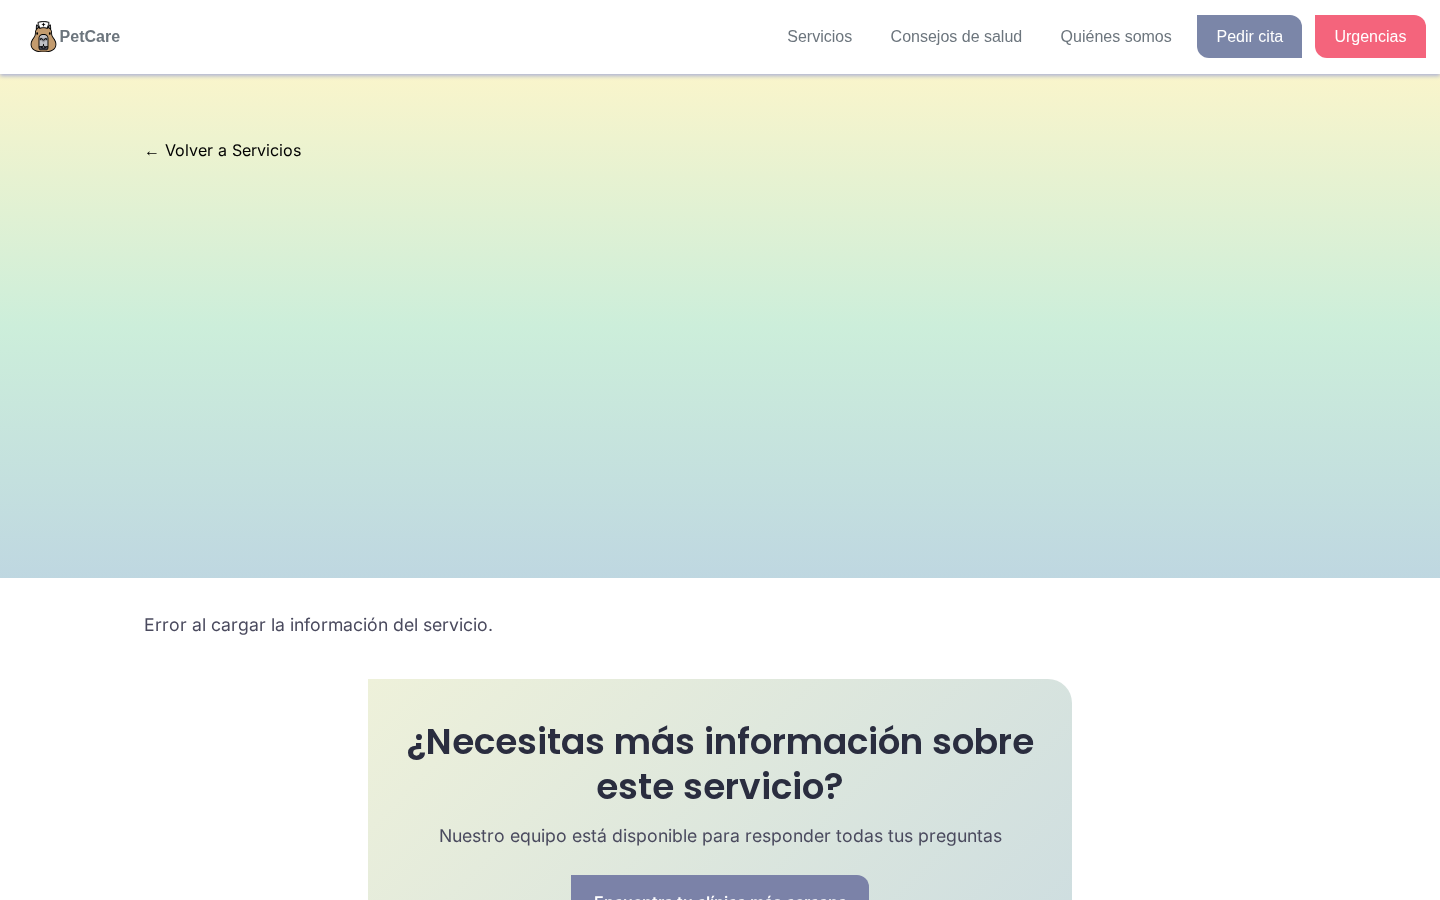
\includegraphics[width=0.85\textheight,keepaspectratio]{capturas_responsivas/servicio-especifico-desktop.png}}
\caption{Servicio específico --- escritorio}
\end{figure}

\begin{figure}[H]
\centering
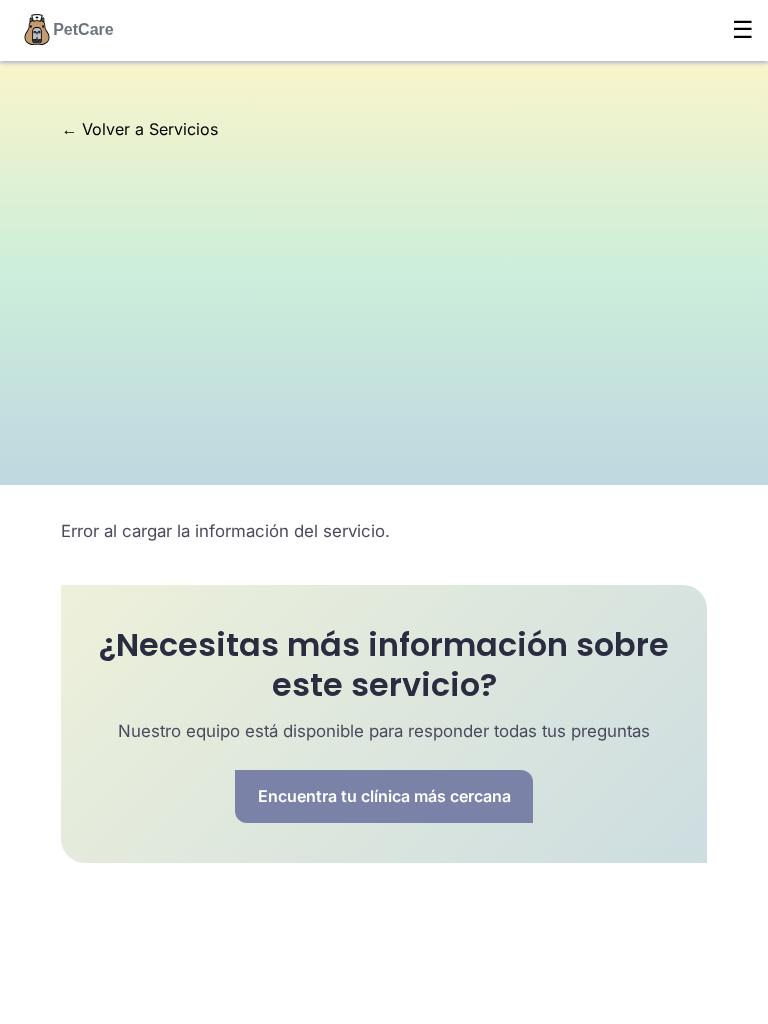
\includegraphics[width=0.70\linewidth,height=0.65\textheight,keepaspectratio]{capturas_responsivas/servicio-especifico-tablet.png}
\caption{Servicio específico --- tablet}
\end{figure}

\begin{figure}[H]
\centering

\includegraphics[width=0.38\linewidth,height=0.65\textheight,keepaspectratio]{capturas_responsivas/servicio-especifico-mobile.png}
\caption{Servicio específico --- móvil}
\end{figure}

\clearpage

% ─────────────────────────────────────────────────────────────────────────────
\subsection{Consejos de salud}
% ─────────────────────────────────────────────────────────────────────────────

\begin{figure}[H]
\centering
\rotatebox{90}{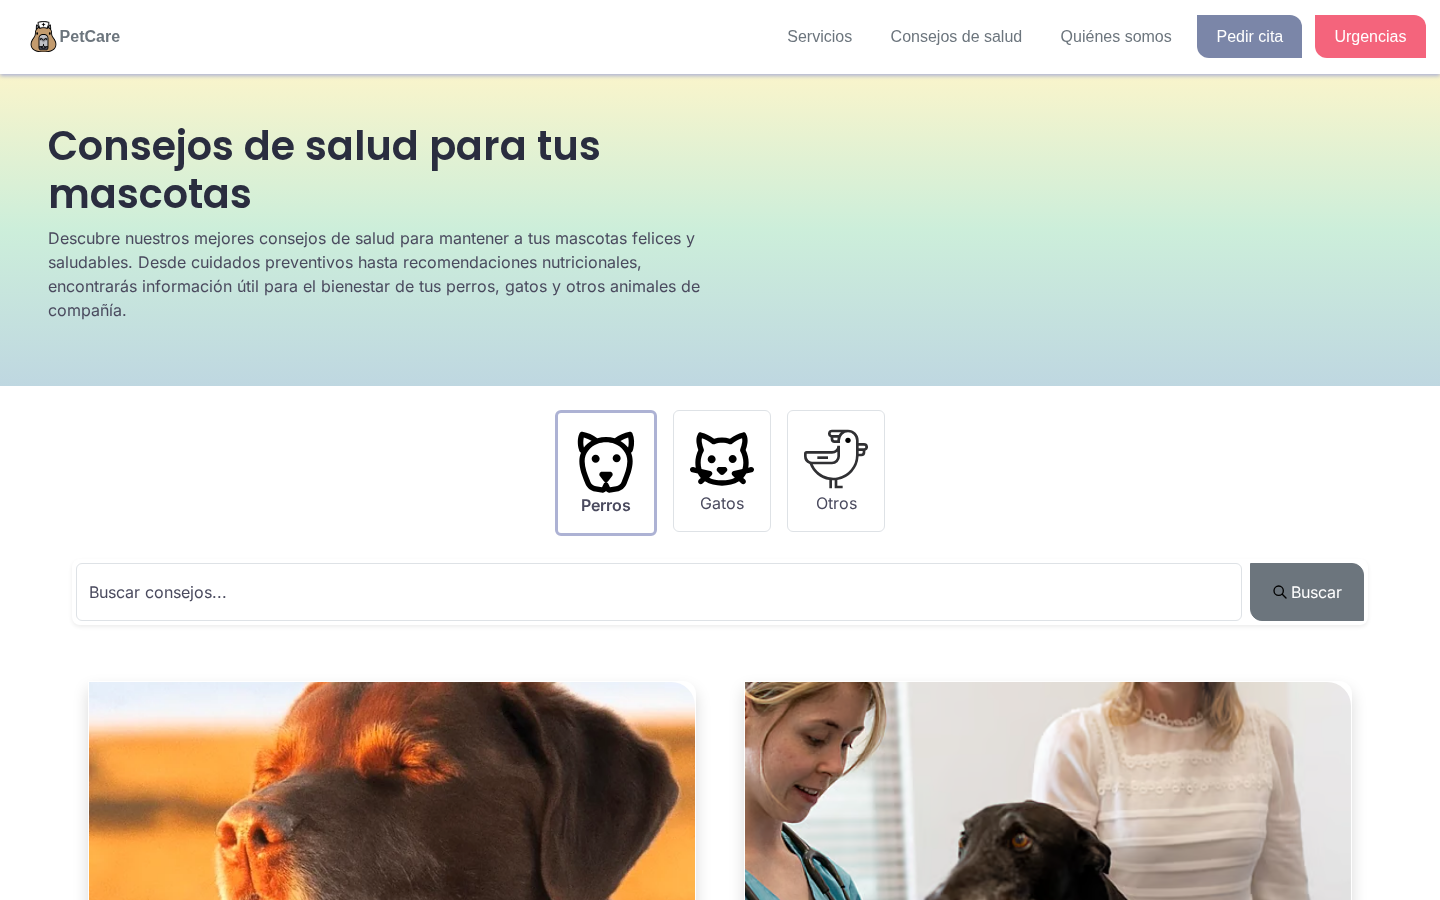
\includegraphics[width=0.85\textheight,keepaspectratio]{capturas_responsivas/consejos-desktop.png}}
\caption{Consejos de salud --- escritorio}
\end{figure}

\begin{figure}[H]
\centering
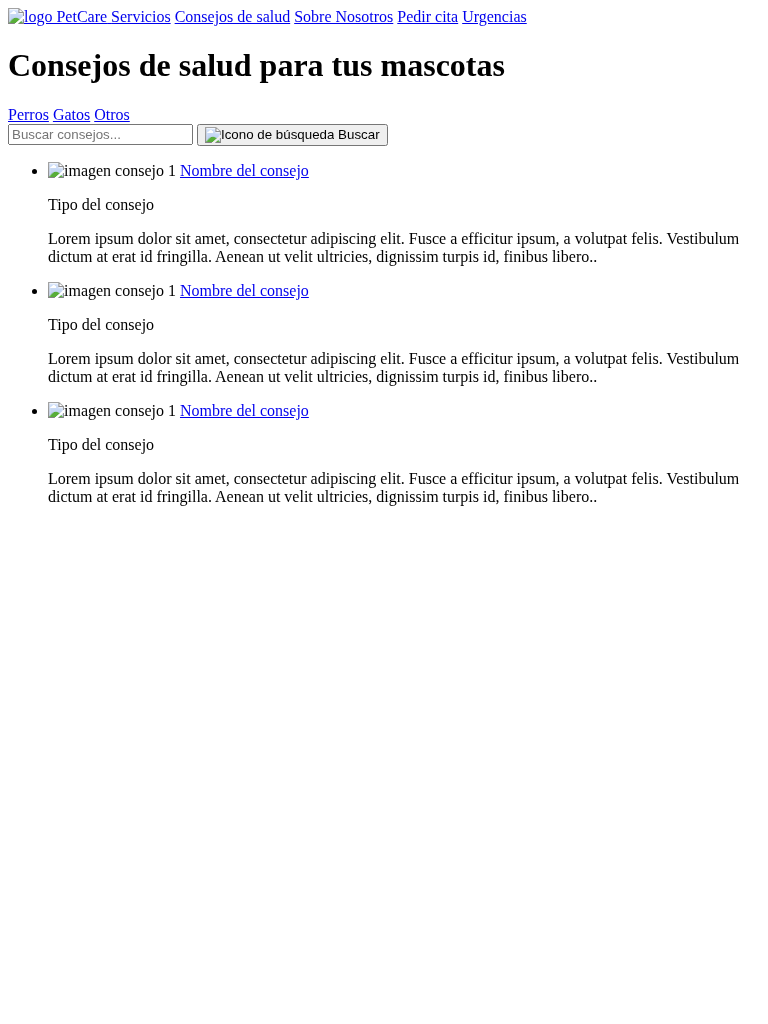
\includegraphics[width=0.70\linewidth,height=0.65\textheight,keepaspectratio]{capturas_responsivas/consejos-tablet.png}
\caption{Consejos de salud --- tablet}
\end{figure}

\begin{figure}[H]
\centering
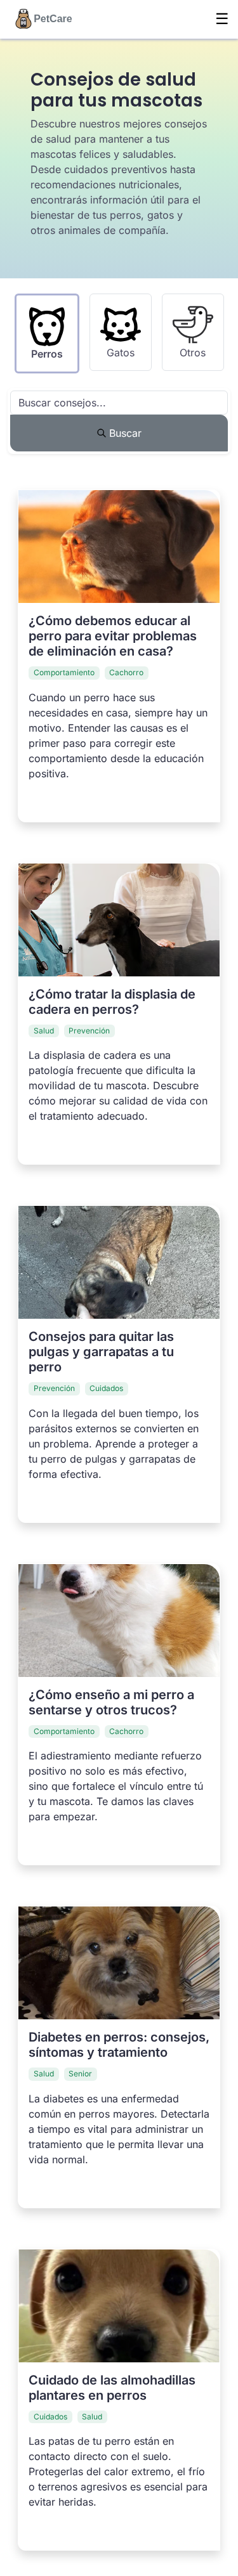
\includegraphics[width=0.38\linewidth,height=0.65\textheight,keepaspectratio]{capturas_responsivas/consejos-mobile.png}
\caption{Consejos de salud --- móvil}
\end{figure}

\clearpage

% ─────────────────────────────────────────────────────────────────────────────
\subsection{Consejo específico}
% ─────────────────────────────────────────────────────────────────────────────

\begin{figure}[H]
\centering
\rotatebox{90}{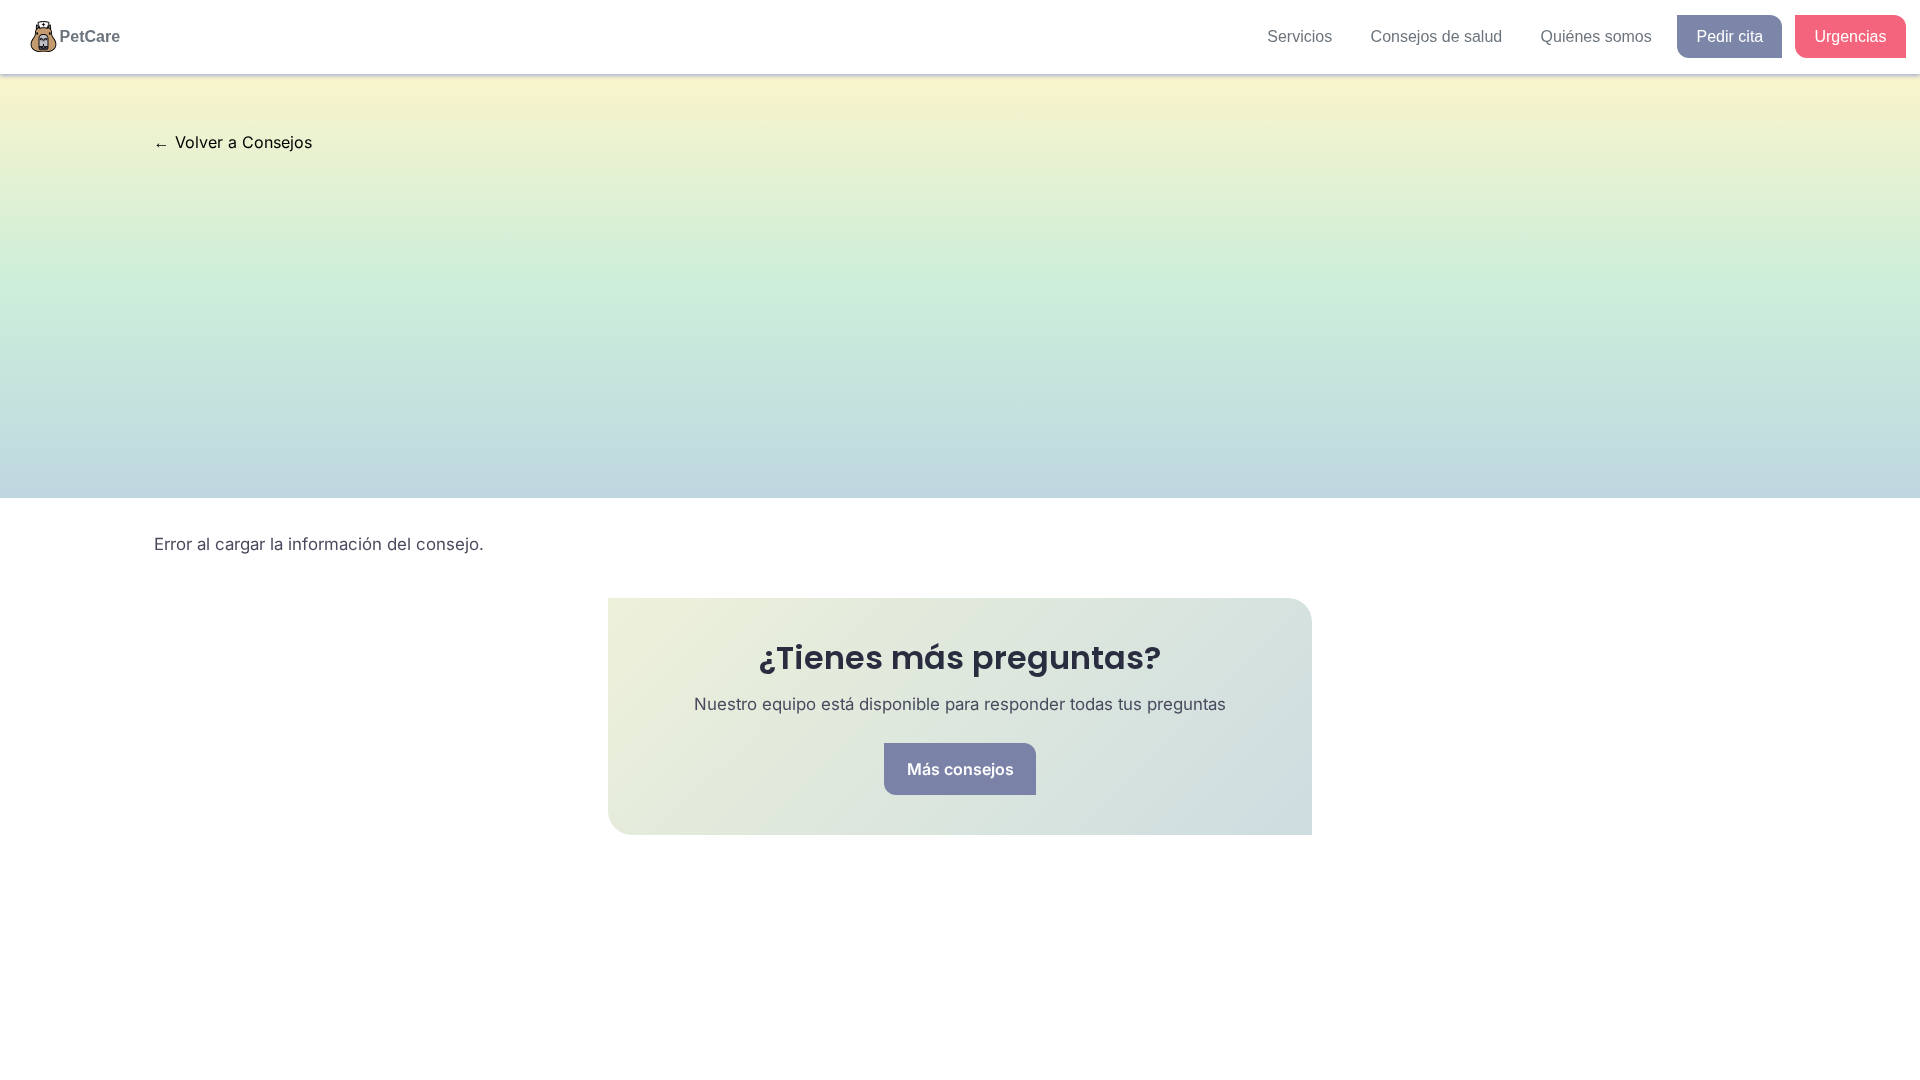
\includegraphics[width=0.85\textheight,keepaspectratio]{capturas_responsivas/consejo-especifico-desktop.png}}
\caption{Consejo específico --- escritorio}
\end{figure}

\begin{figure}[H]
\centering

\includegraphics[width=0.70\linewidth,height=0.65\textheight,keepaspectratio]{capturas_responsivas/consejo-especifico-tablet.png}
\caption{Consejo específico --- tablet}
\end{figure}

\begin{figure}[H]
\centering
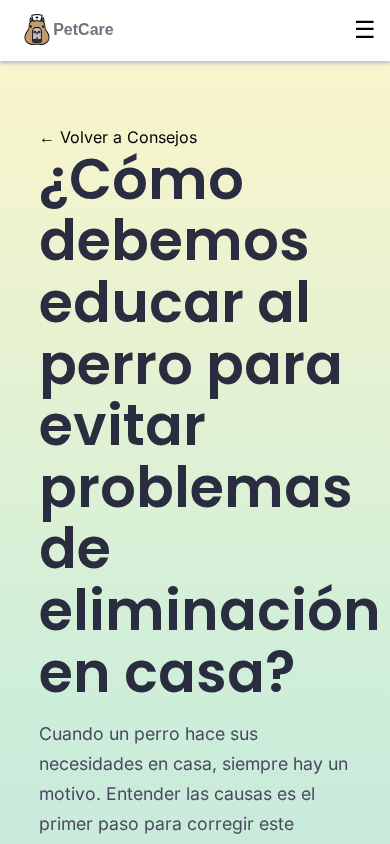
\includegraphics[width=0.38\linewidth,height=0.65\textheight,keepaspectratio]{capturas_responsivas/consejo-especifico-mobile.png}
\caption{Consejo específico --- móvil}
\end{figure}

\clearpage

% ─────────────────────────────────────────────────────────────────────────────
\subsection{Sobre nosotros}
% ─────────────────────────────────────────────────────────────────────────────

\begin{figure}[H]
\centering
\rotatebox{90}{
\includegraphics[width=0.85\textheight,keepaspectratio]{capturas_responsivas/sobre-nosotros-desktop.png}}
\caption{Sobre nosotros --- escritorio}
\end{figure}

\begin{figure}[H]
\centering
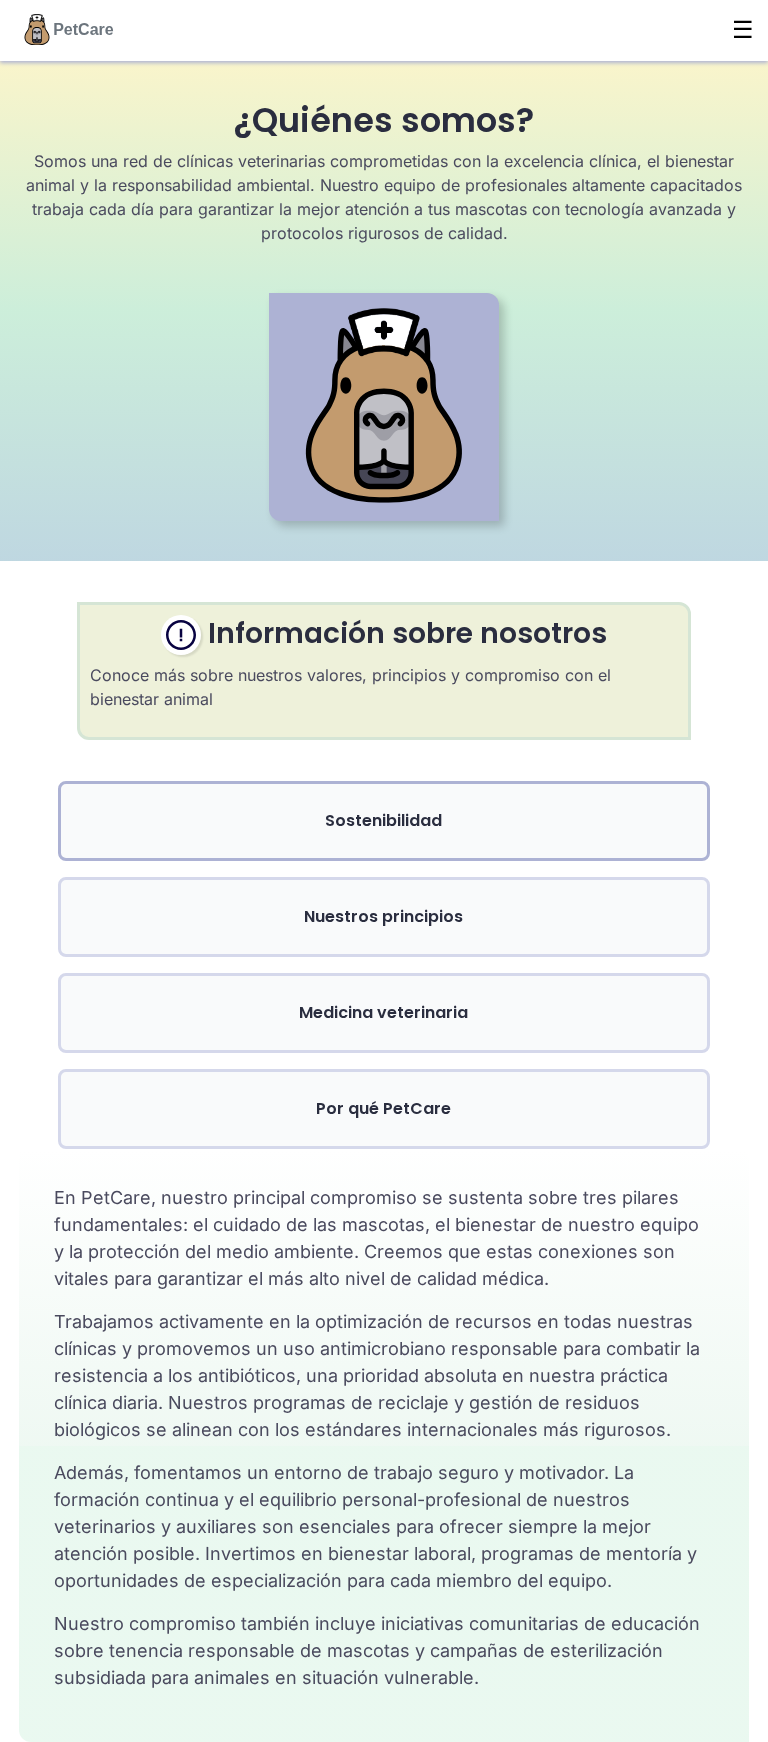
\includegraphics[width=0.70\linewidth,height=0.65\textheight,keepaspectratio]{capturas_responsivas/sobre-nosotros-tablet.png}
\caption{Sobre nosotros --- tablet}
\end{figure}

\begin{figure}[H]
\centering
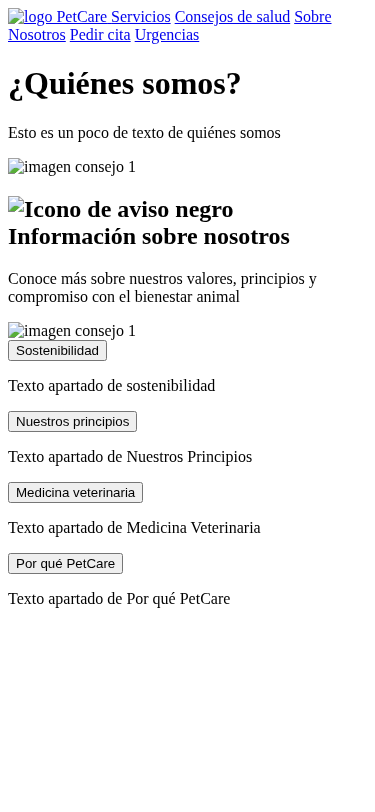
\includegraphics[width=0.38\linewidth,height=0.65\textheight,keepaspectratio]{capturas_responsivas/sobre-nosotros-mobile.png}
\caption{Sobre nosotros --- móvil}
\end{figure}

\clearpage

% ─────────────────────────────────────────────────────────────────────────────
\subsection{Solicitud de cita}
% ─────────────────────────────────────────────────────────────────────────────

\begin{figure}[H]
\centering
\rotatebox{90}{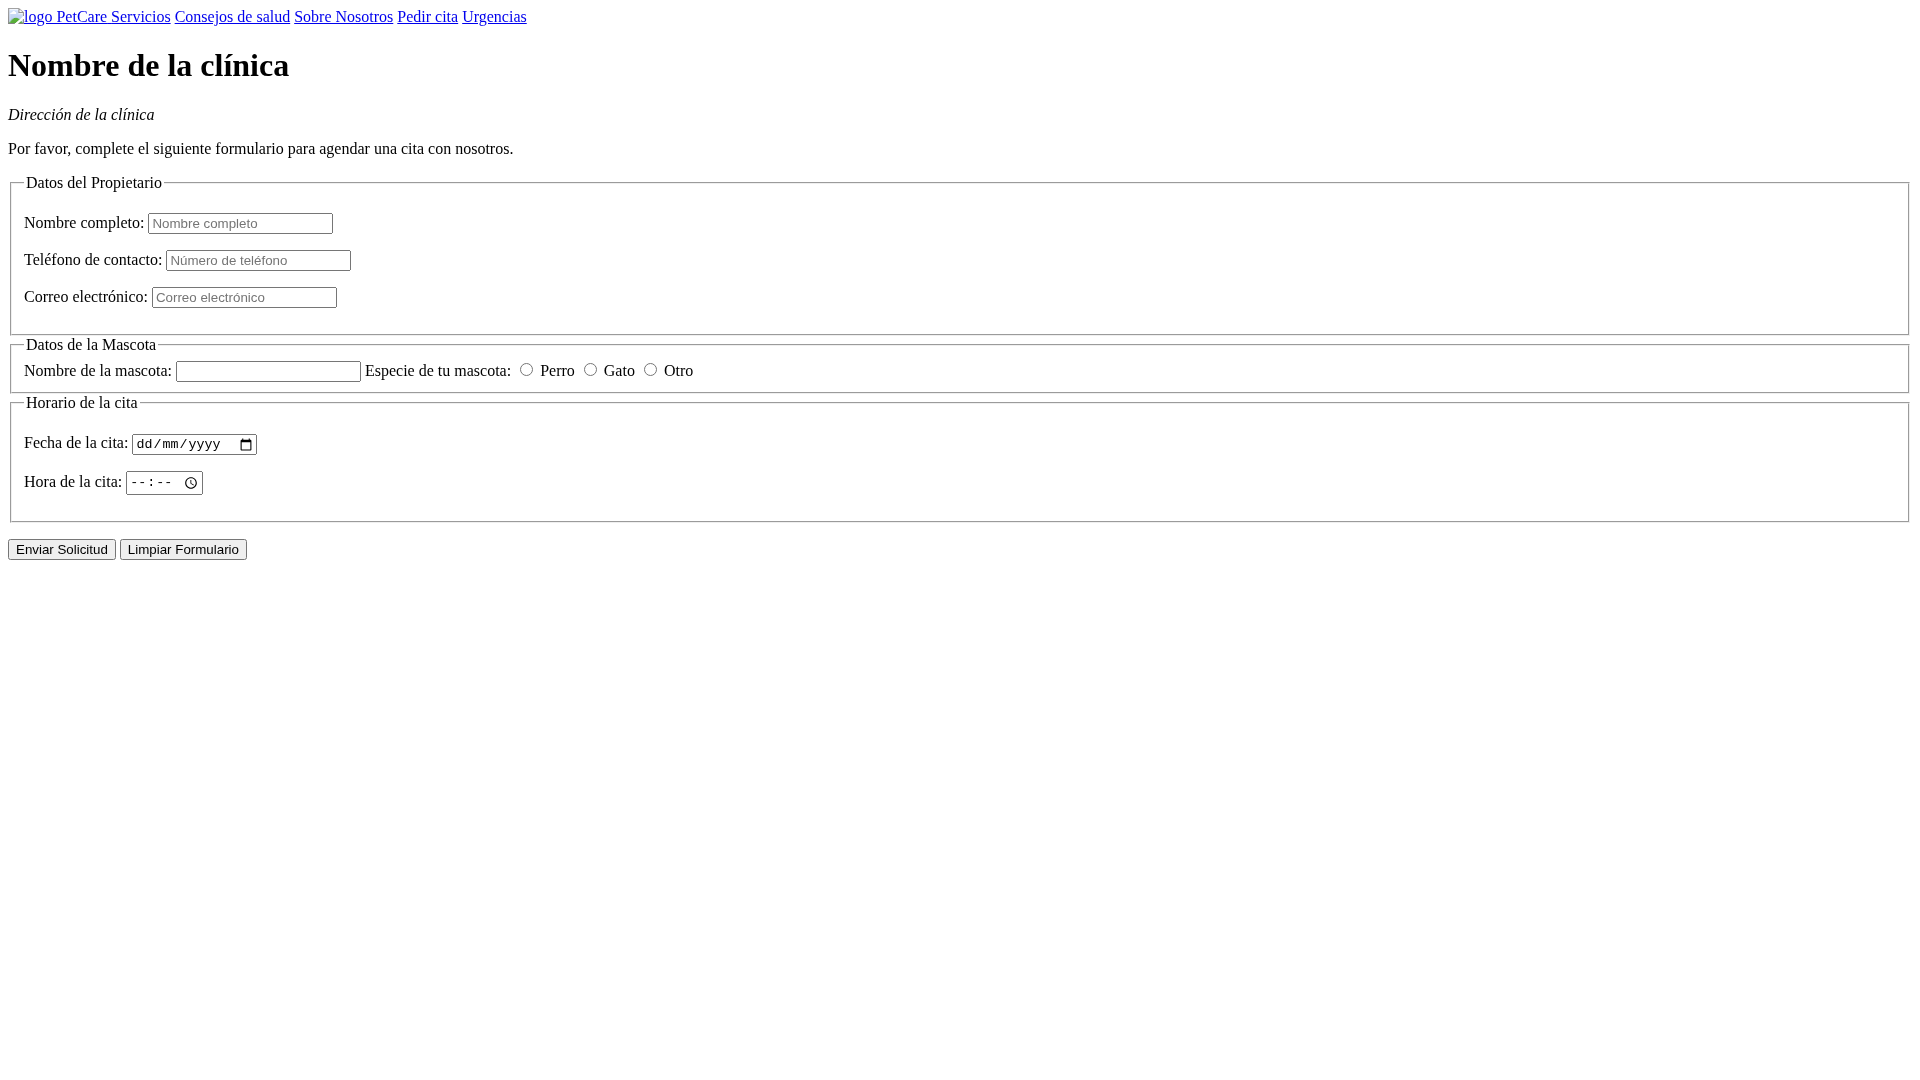
\includegraphics[width=0.85\textheight,keepaspectratio]{capturas_responsivas/pedir-cita-desktop.png}}
\caption{Solicitud de cita --- escritorio}
\end{figure}

\begin{figure}[H]
\centering
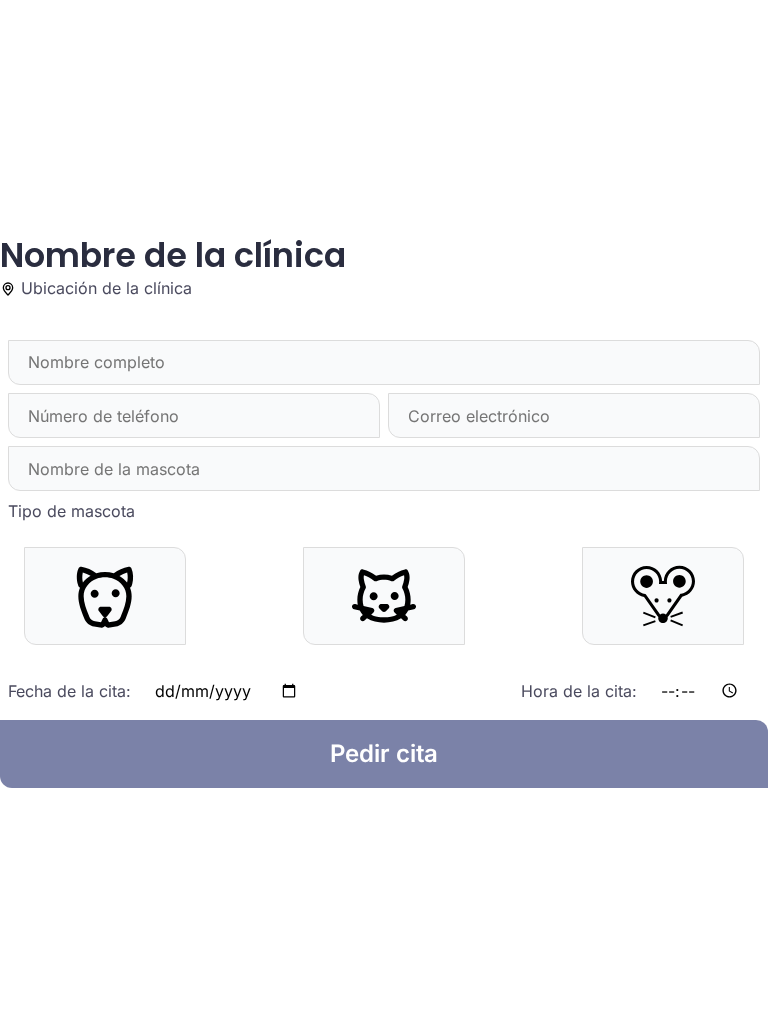
\includegraphics[width=0.70\linewidth,height=0.65\textheight,keepaspectratio]{capturas_responsivas/pedir-cita-tablet.png}
\caption{Solicitud de cita --- tablet}
\end{figure}

\begin{figure}[H]
\centering
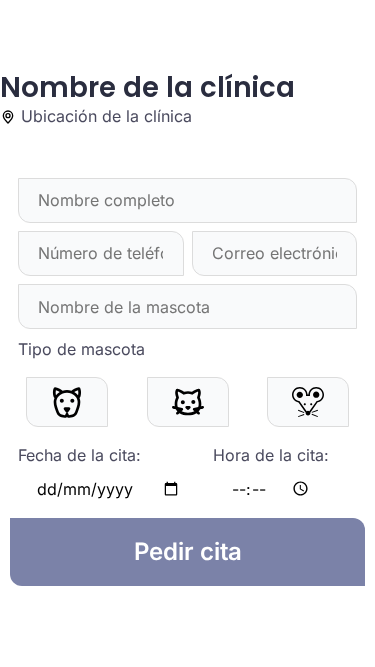
\includegraphics[width=0.38\linewidth,height=0.65\textheight,keepaspectratio]{capturas_responsivas/pedir-cita-mobile.png}
\caption{Solicitud de cita --- móvil}
\end{figure}

clearpage

% ─────────────────────────────────────────────────────────────────────────────
\section{Mapas de Etiquetas y Modificaciones Estructurales}
% ─────────────────────────────────────────────────────────────────────────────
El presente apéndice recopila la comparativa del árbol del DOM (Document Object Model) de todas las rutas que componen la aplicación. A la izquierda se presenta el mapa de bloques base, y a la derecha se ilustran las modificaciones estructurales introducidas en la Práctica 3. Los elementos resaltados en verde denotan la inyección de nuevas etiquetas, mientras que los elementos con borde discontinuo naranja indican la modificación de sus atributos (principalmente para la inclusión de clases de utilidad responsiva o \textit{frameworks} externos).

\vspace{1em}

\begin{figure}[H]
    \centering
    \begin{minipage}{0.48\textwidth}
        \centering
        
\includegraphics[width=\linewidth,keepaspectratio]{mapasDeEtiquetas/index-boxmodel.png}
        \caption{Página de inicio (Base)}
    \end{minipage}\hfill
    \begin{minipage}{0.48\textwidth}
        \centering
        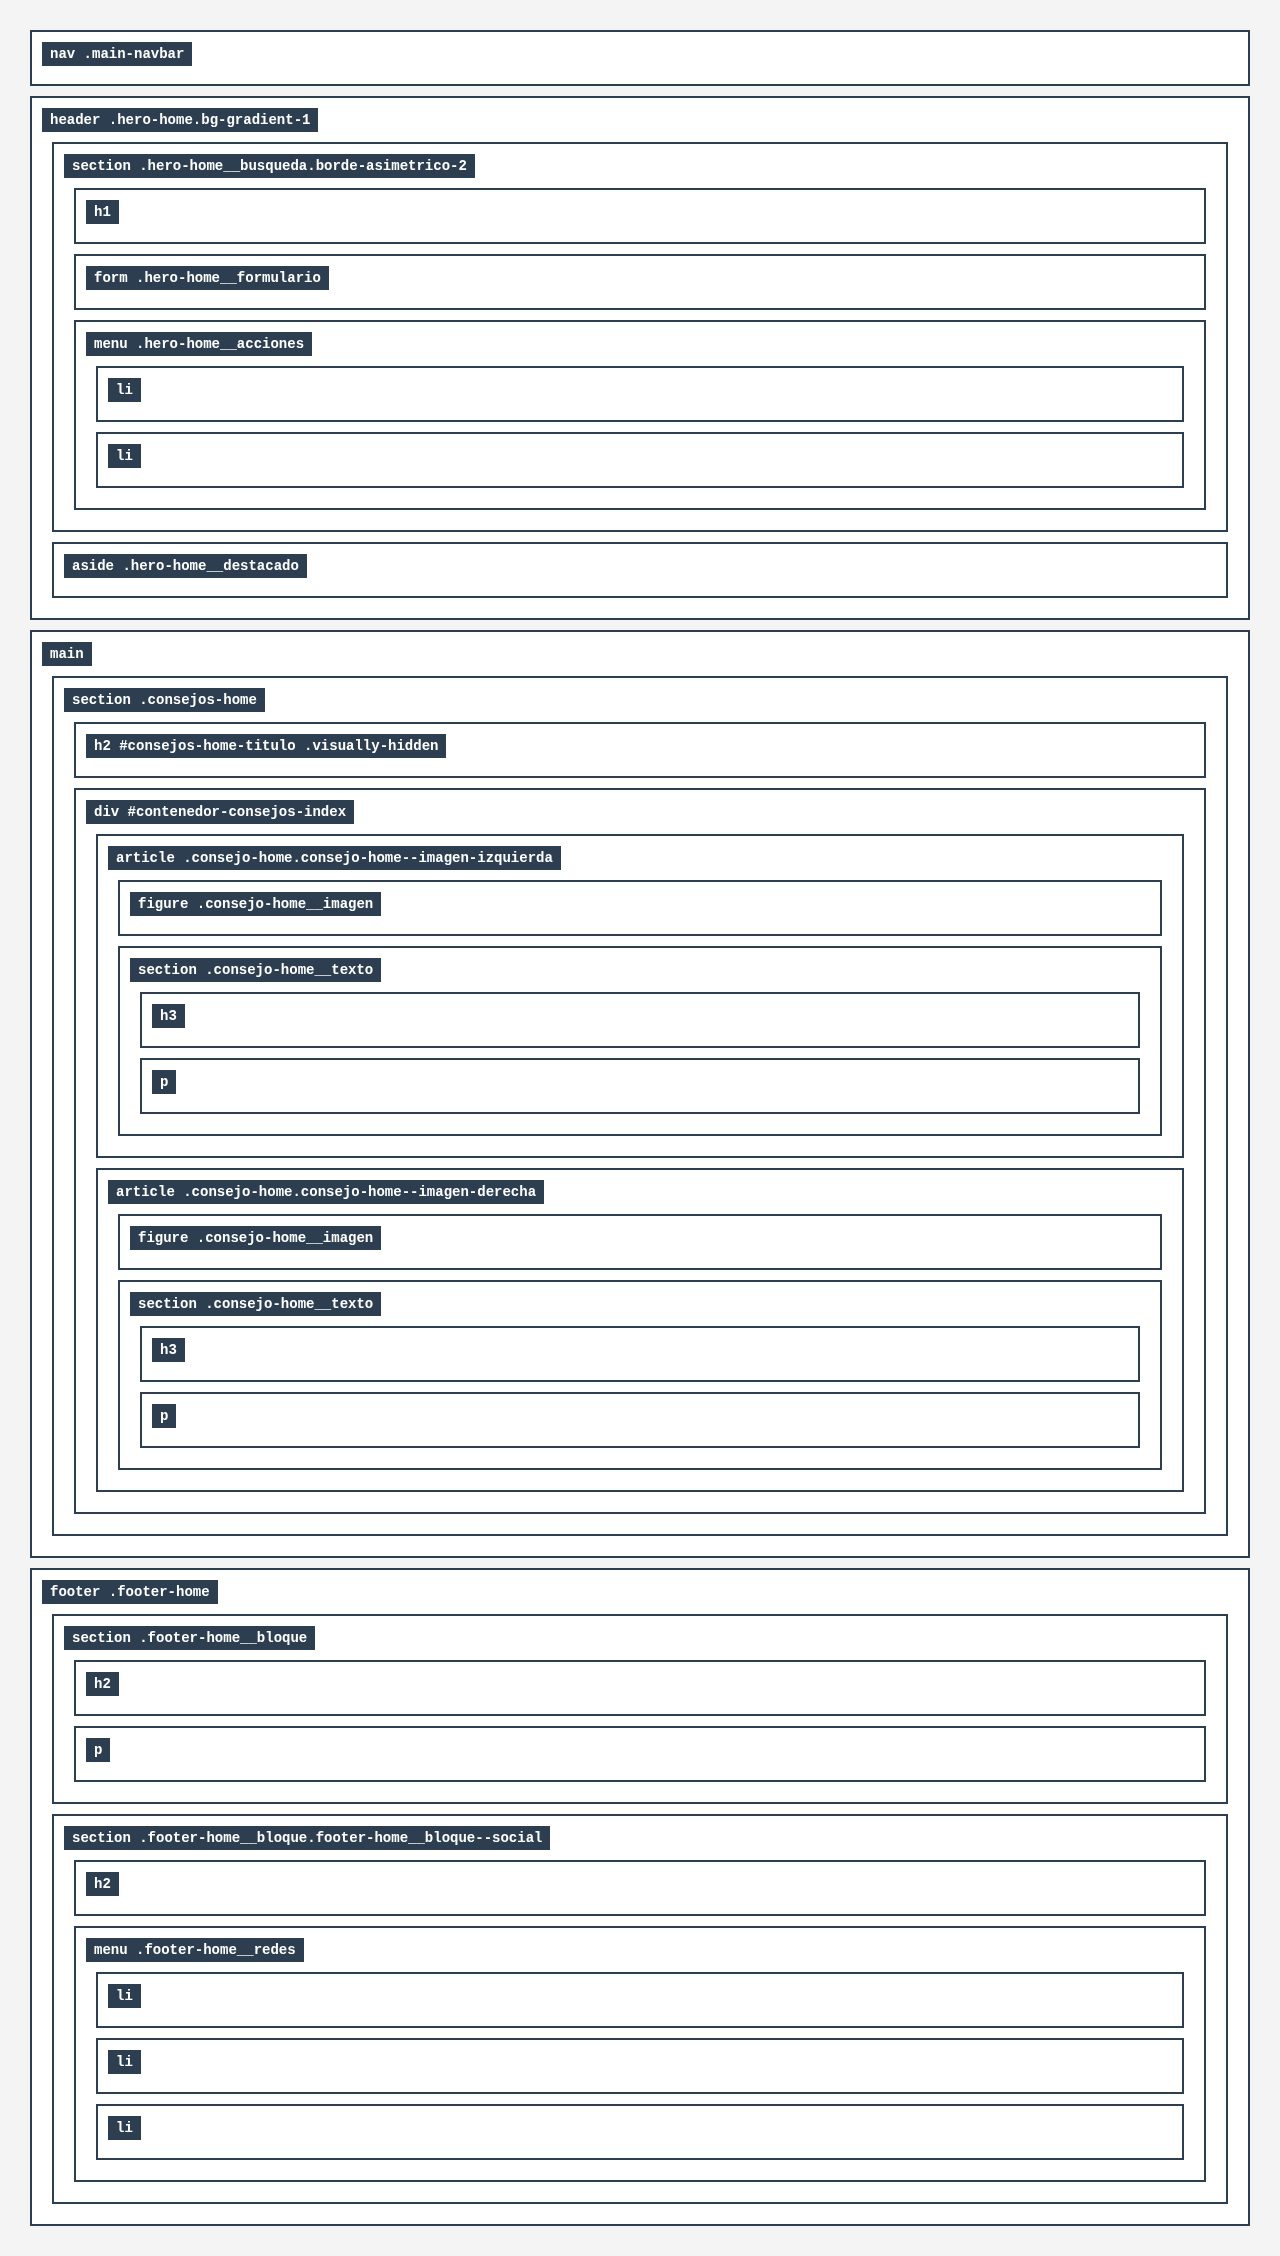
\includegraphics[width=\linewidth,keepaspectratio]{mapasDeEtiquetas/index-boxmodel-new.png}
        \caption{Página de inicio (Cambios)}
    \end{minipage}
\end{figure}

\begin{figure}[H]
    \centering
    \begin{minipage}{0.48\textwidth}
        \centering
        
\includegraphics[width=\linewidth,keepaspectratio]{mapasDeEtiquetas/clinicas-boxmodel.png}
        \caption{Clínicas (Base)}
    \end{minipage}\hfill
    \begin{minipage}{0.48\textwidth}
        \centering
        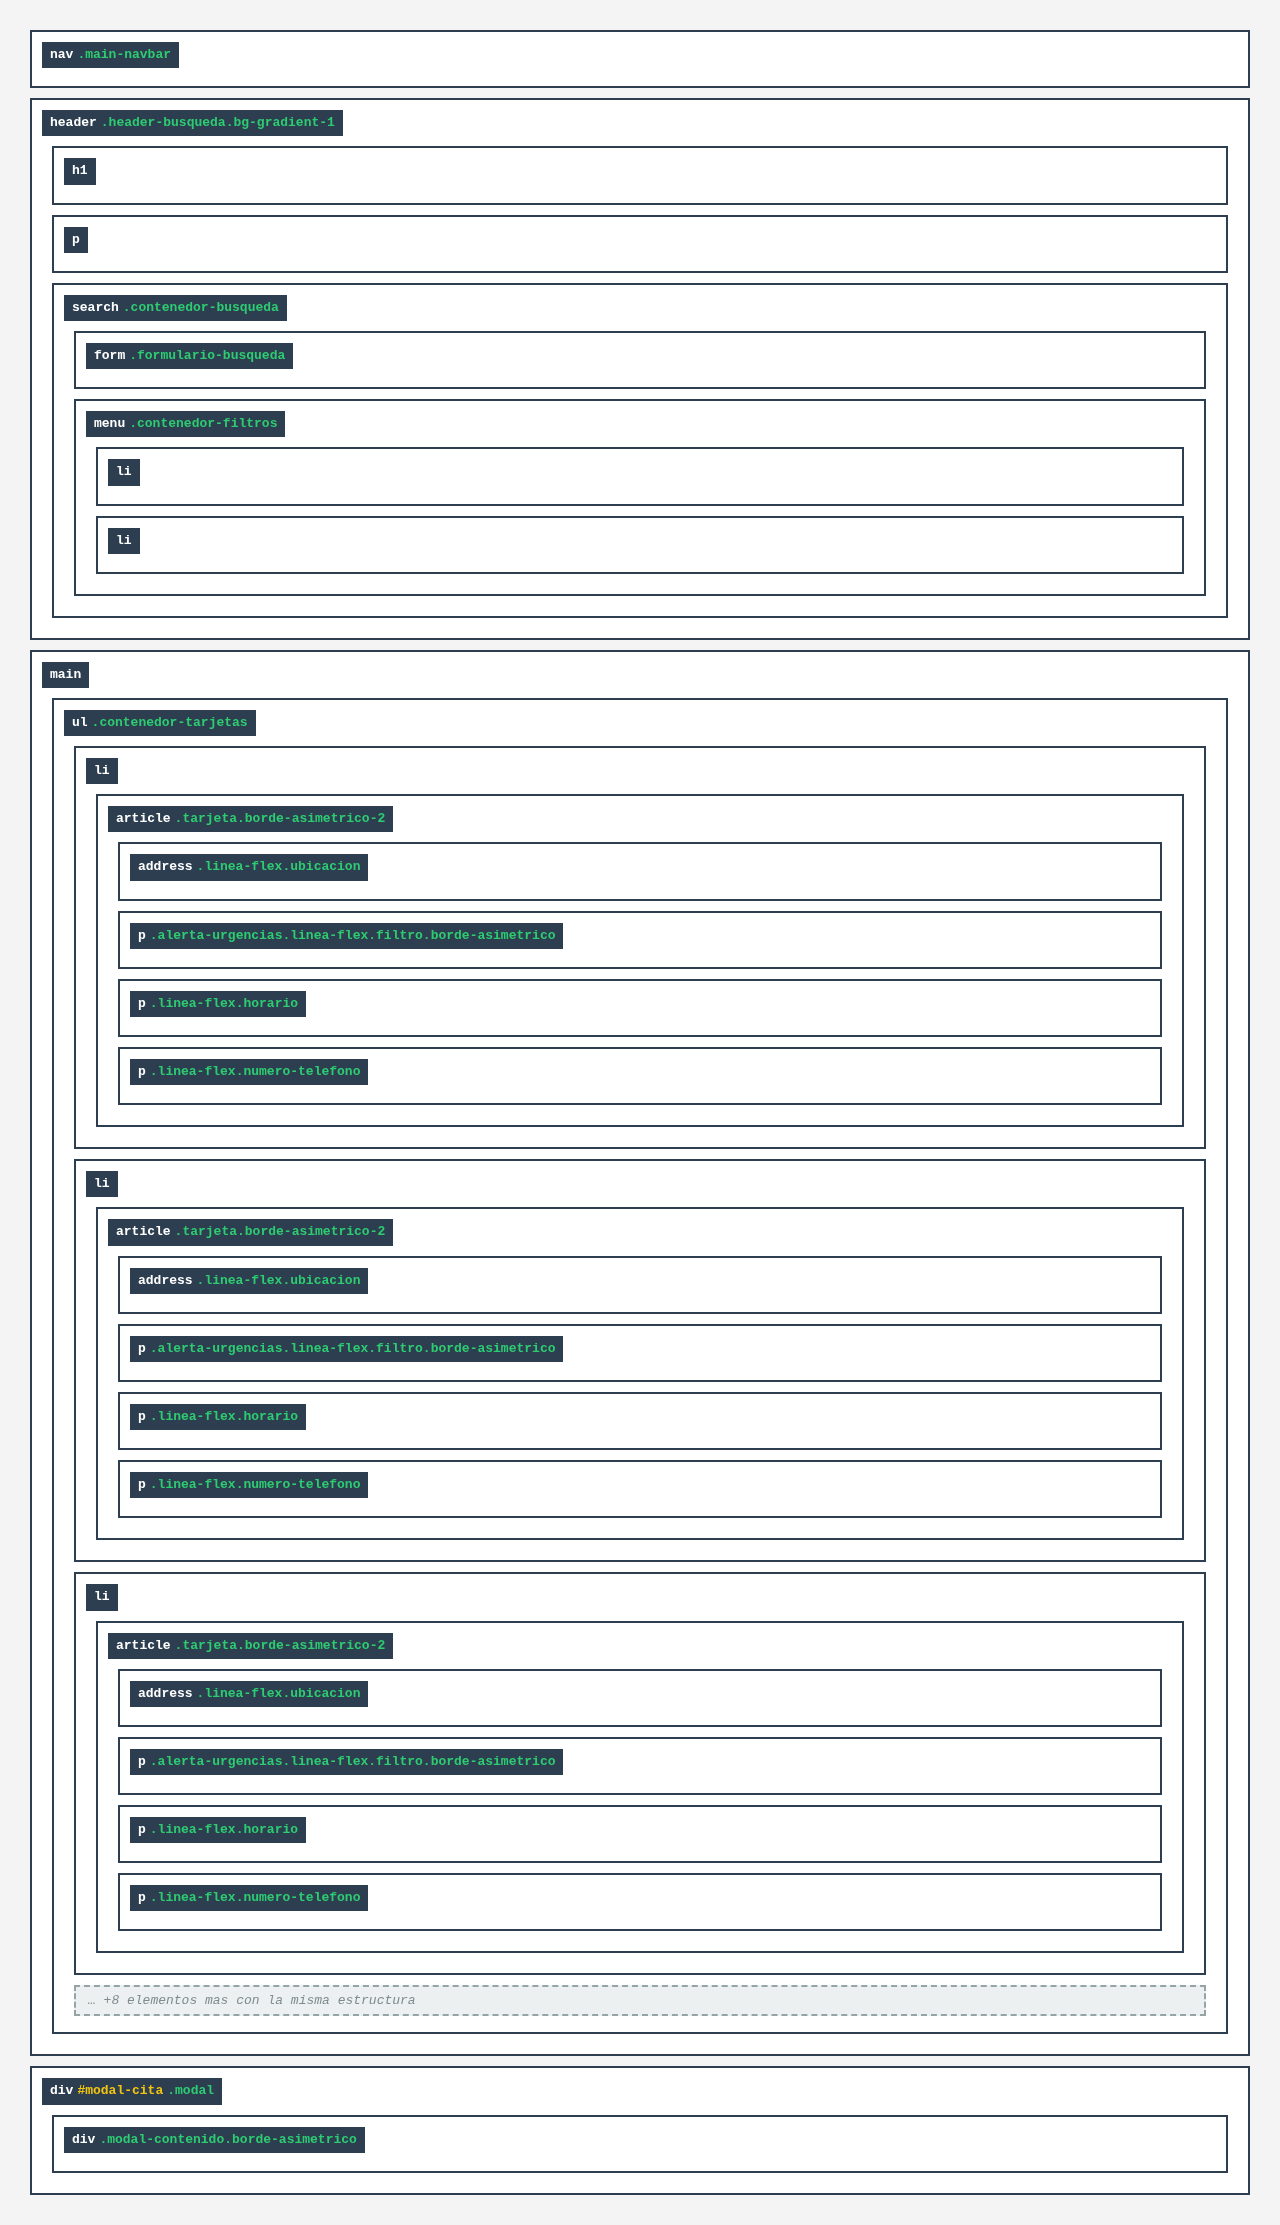
\includegraphics[width=\linewidth,keepaspectratio]{mapasDeEtiquetas/clinicas-boxmodel-new.png}
        \caption{Clínicas (Cambios)}
    \end{minipage}
\end{figure}

\begin{figure}[H]
    \centering
    \begin{minipage}{0.48\textwidth}
        \centering
        
\includegraphics[width=\linewidth,keepaspectratio]{mapasDeEtiquetas/servicios-boxmodel.png}
        \caption{Servicios (Base)}
    \end{minipage}\hfill
    \begin{minipage}{0.48\textwidth}
        \centering
        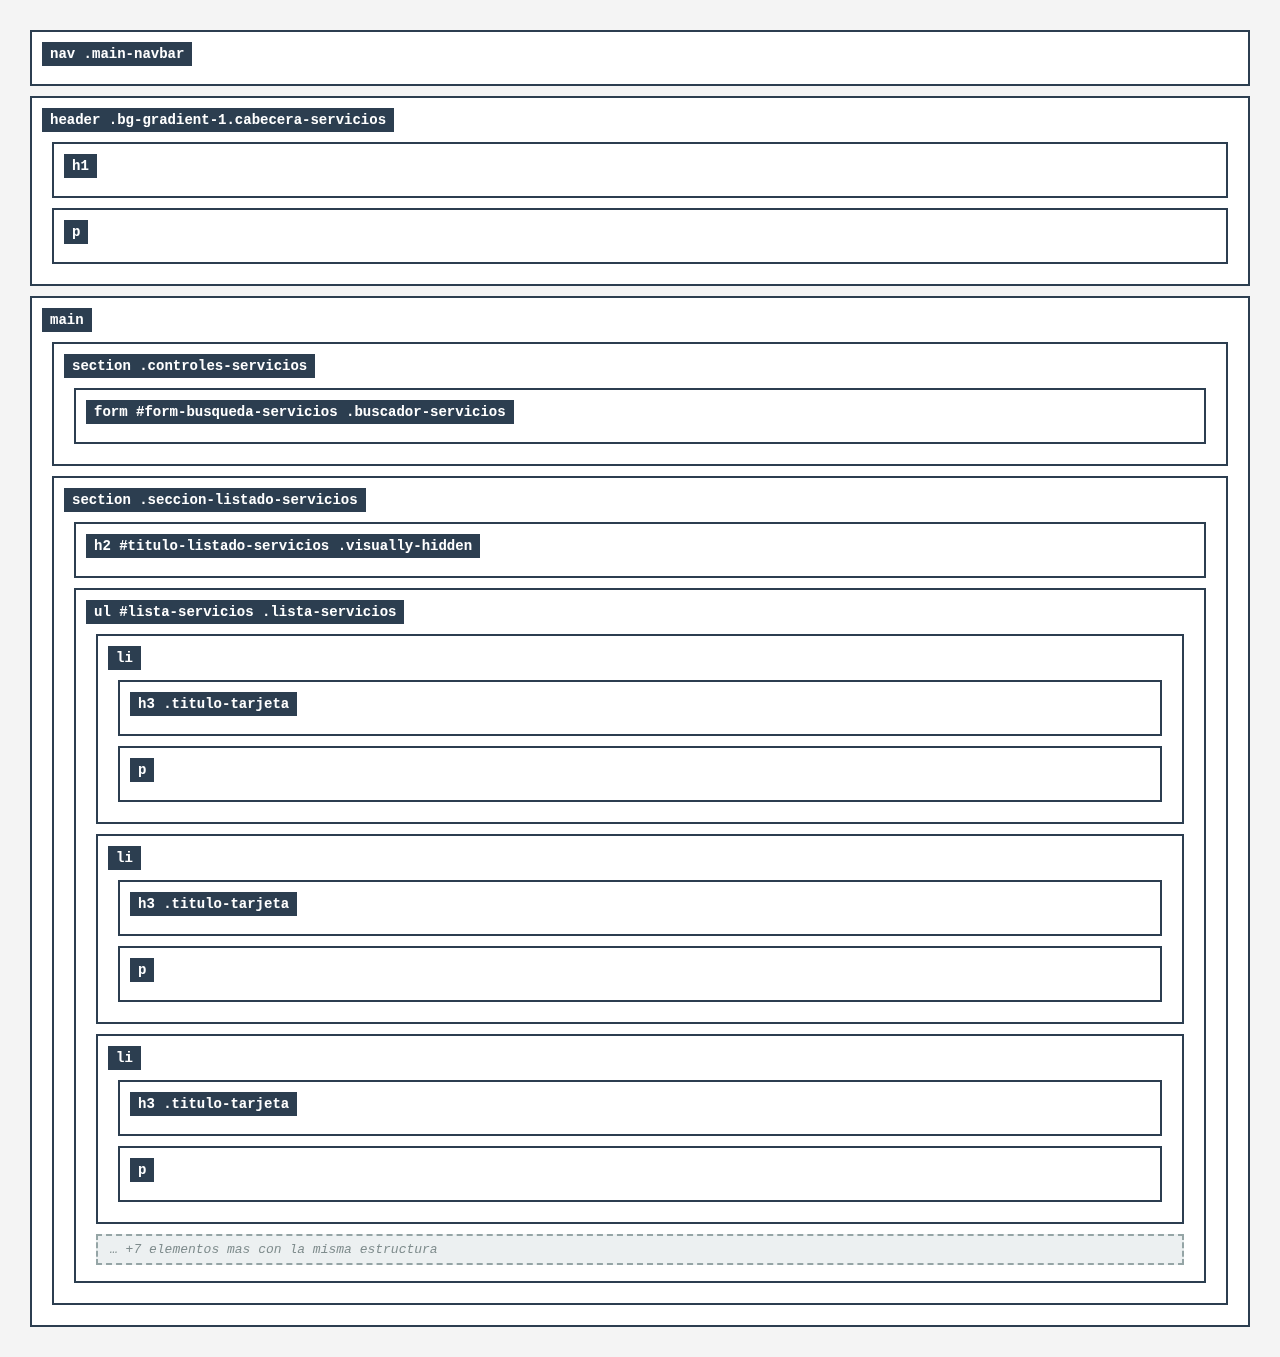
\includegraphics[width=\linewidth,keepaspectratio]{mapasDeEtiquetas/servicios-boxmodel-new.png}
        \caption{Servicios (Cambios)}
    \end{minipage}
\end{figure}

\begin{figure}[H]
    \centering
    \begin{minipage}{0.48\textwidth}
        \centering
        
\includegraphics[width=\linewidth,keepaspectratio]{mapasDeEtiquetas/servicio-especifico-boxmodel.png}
        \caption{Servicio específico (Base)}
    \end{minipage}\hfill
    \begin{minipage}{0.48\textwidth}
        \centering
        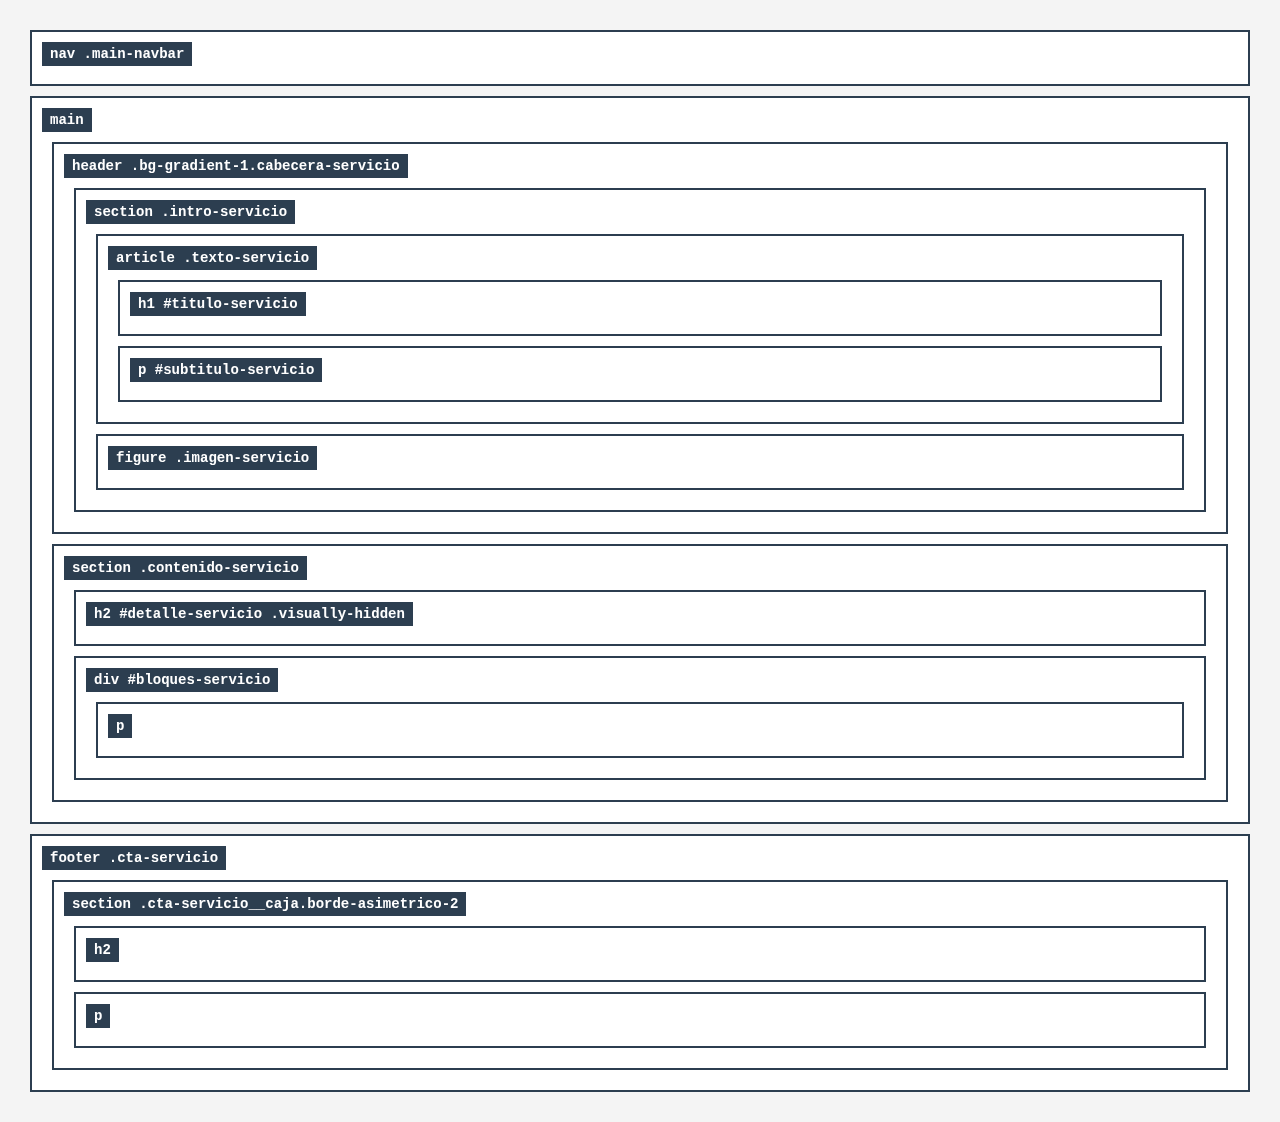
\includegraphics[width=\linewidth,keepaspectratio]{mapasDeEtiquetas/servicio-especifico-boxmodel-new.png}
        \caption{Servicio específico (Cambios)}
    \end{minipage}
\end{figure}

\begin{figure}[H]
    \centering
    \begin{minipage}{0.48\textwidth}
        \centering
        
\includegraphics[width=\linewidth,keepaspectratio]{mapasDeEtiquetas/consejos-boxmodel.png}
        \caption{Consejos de salud (Base)}
    \end{minipage}\hfill
    \begin{minipage}{0.48\textwidth}
        \centering
        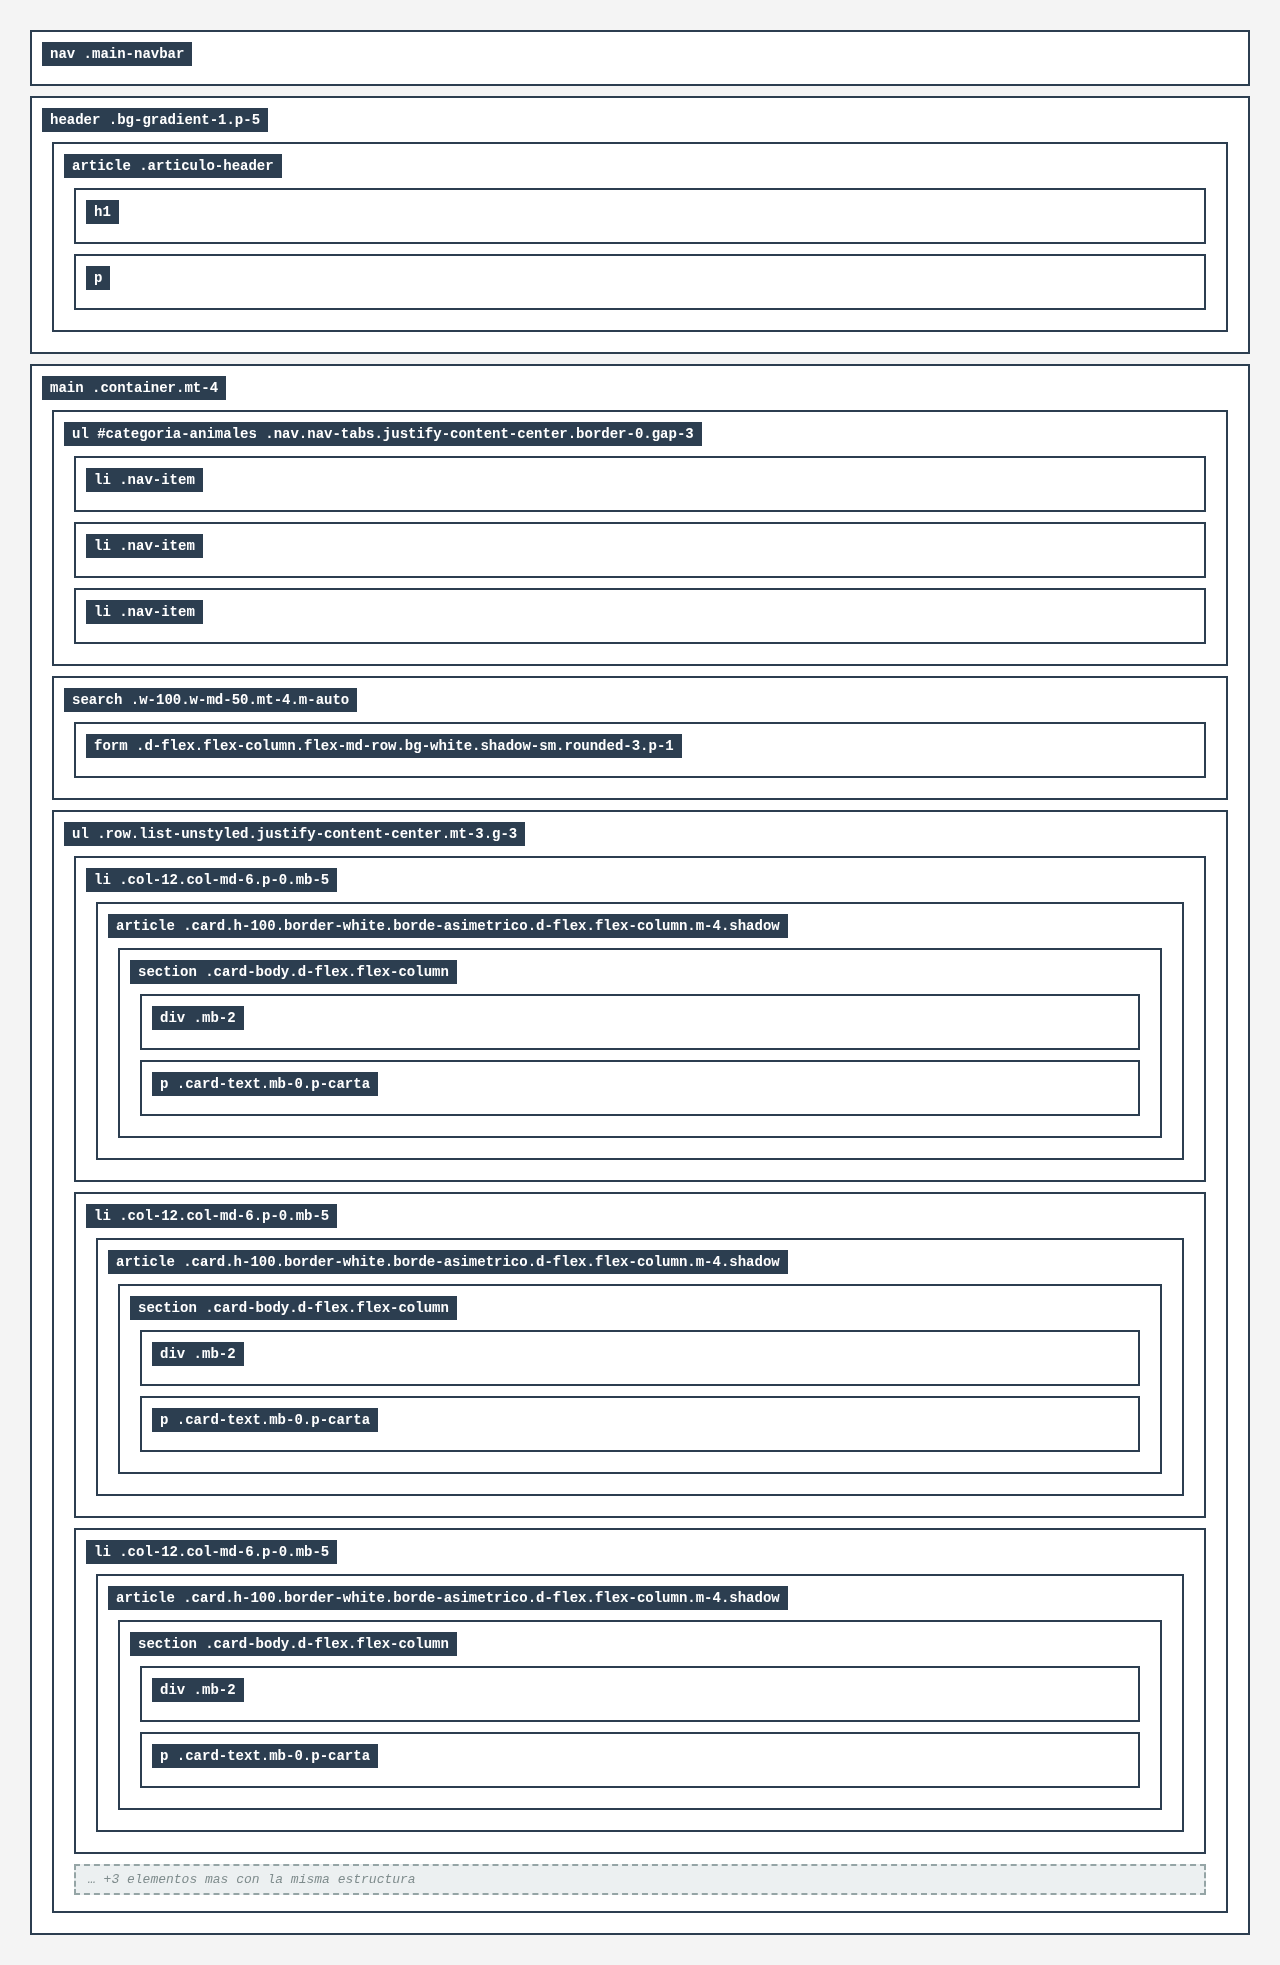
\includegraphics[width=\linewidth,keepaspectratio]{mapasDeEtiquetas/consejos-boxmodel-new.png}
        \caption{Consejos de salud (Cambios)}
    \end{minipage}
\end{figure}

\begin{figure}[H]
    \centering
    \begin{minipage}{0.48\textwidth}
        \centering
        
\includegraphics[width=\linewidth,keepaspectratio]{mapasDeEtiquetas/consejo-especifico-boxmodel.png}
        \caption{Consejo específico (Base)}
    \end{minipage}\hfill
    \begin{minipage}{0.48\textwidth}
        \centering
        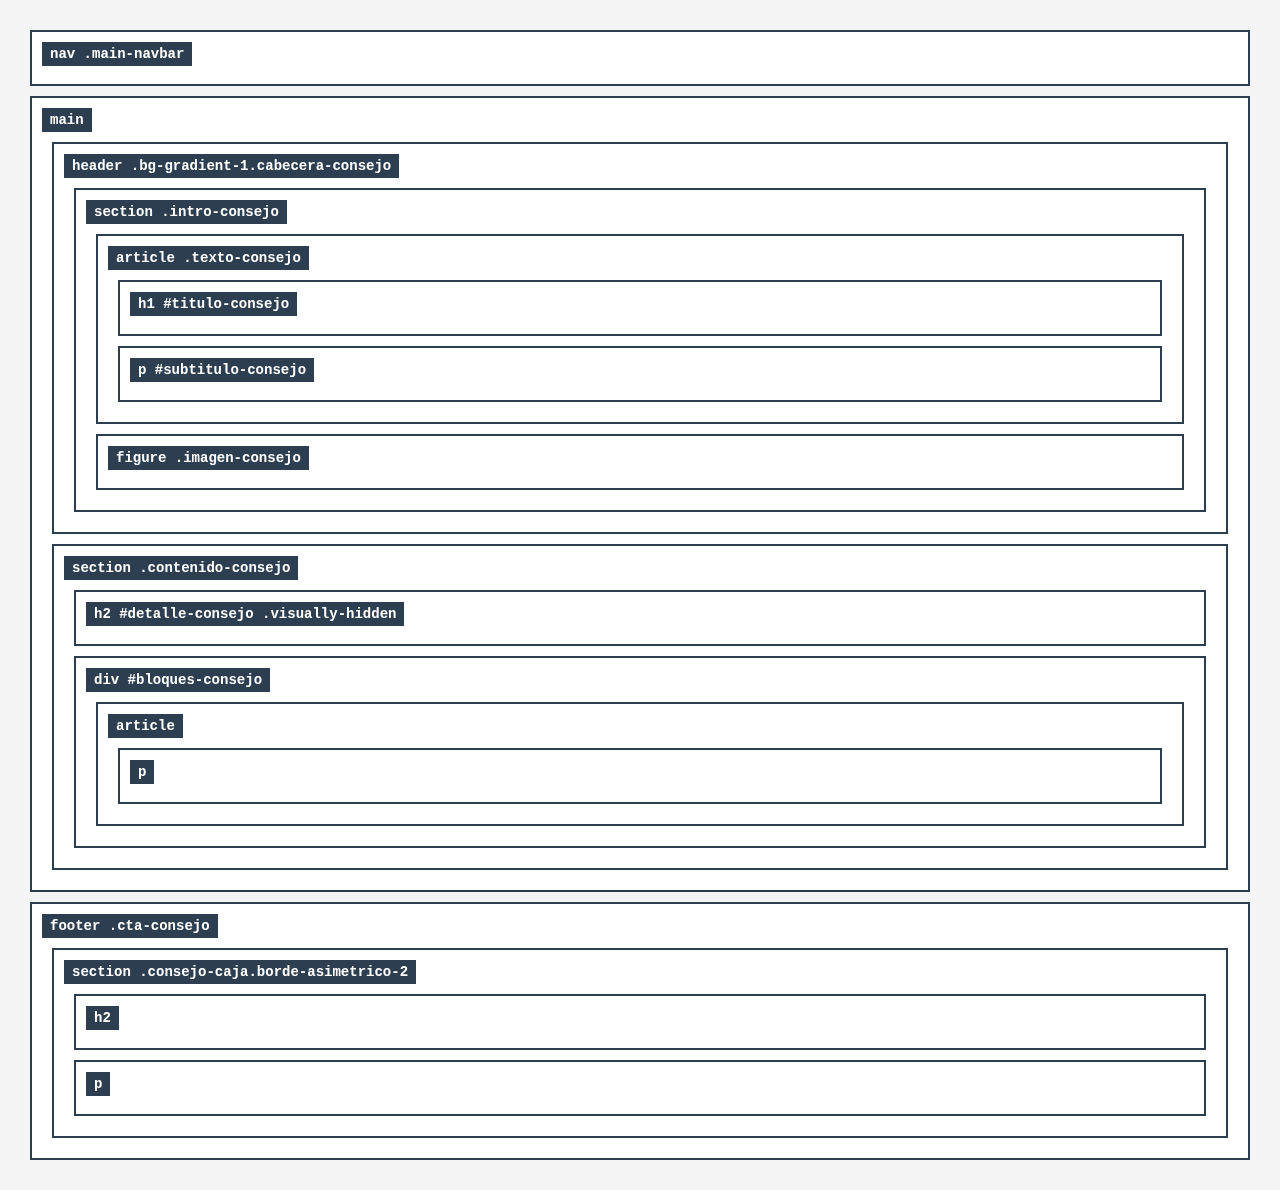
\includegraphics[width=\linewidth,keepaspectratio]{mapasDeEtiquetas/consejo-especifico-boxmodel-new.png}
        \caption{Consejo específico (Cambios)}
    \end{minipage}
\end{figure}

\begin{figure}[H]
    \centering
    \begin{minipage}{0.48\textwidth}
        \centering
        
\includegraphics[width=\linewidth,keepaspectratio]{mapasDeEtiquetas/sobre-nosotros-boxmodel.png}
        \caption{Quiénes somos (Base)}
    \end{minipage}\hfill
    \begin{minipage}{0.48\textwidth}
        \centering
        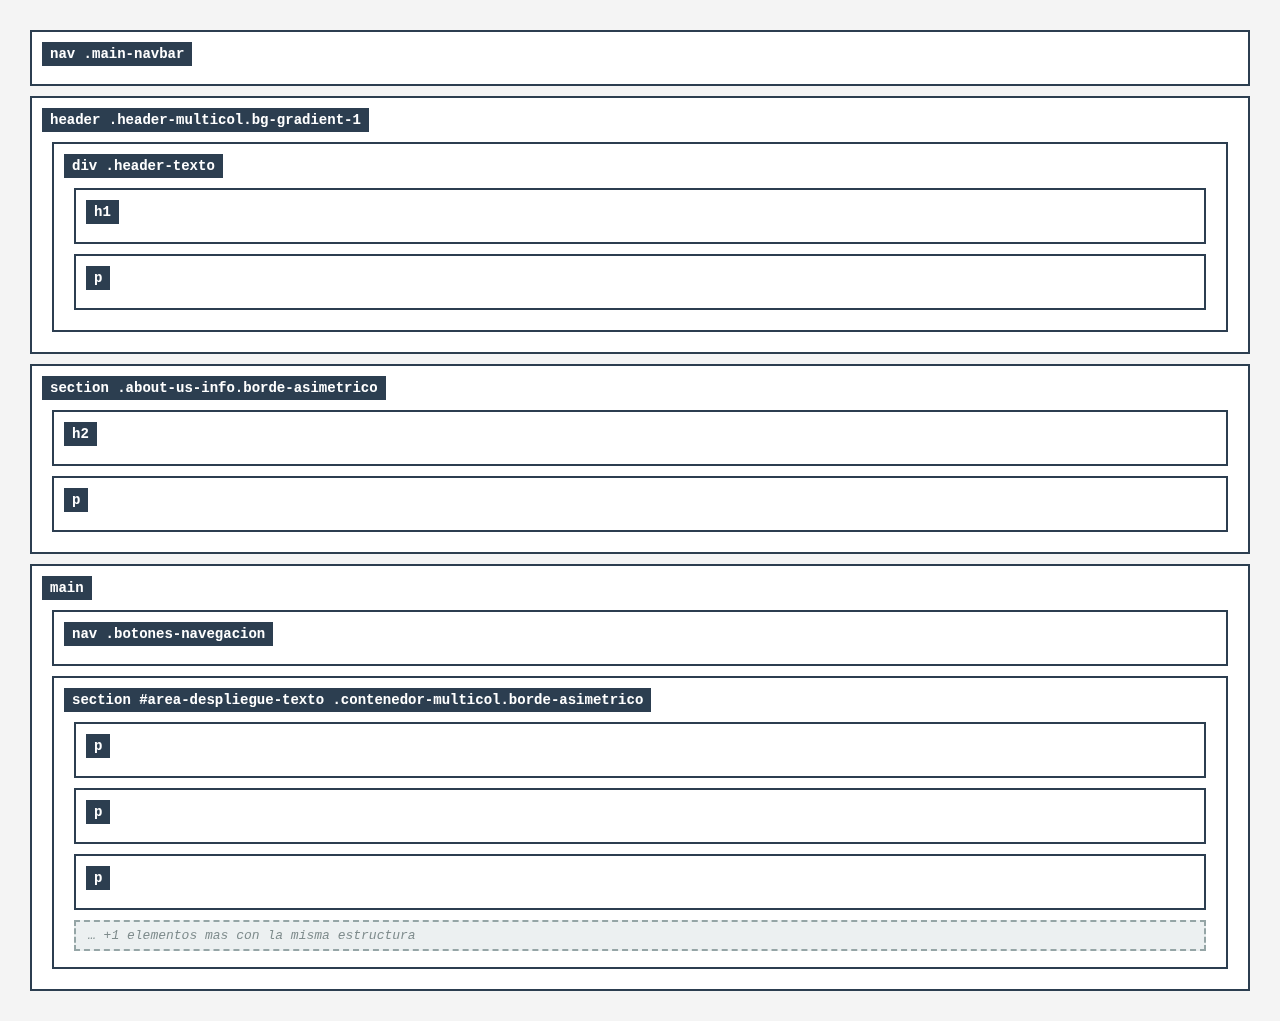
\includegraphics[width=\linewidth,keepaspectratio]{mapasDeEtiquetas/sobre-nosotros-boxmodel-new.png}
        \caption{Quiénes somos (Cambios)}
    \end{minipage}
\end{figure}

\begin{figure}[H]
    \centering
    \begin{minipage}{0.48\textwidth}
        \centering
        
\includegraphics[width=\linewidth,keepaspectratio]{mapasDeEtiquetas/urgencias-boxmodel.png}
        \caption{Urgencias (Base)}
    \end{minipage}\hfill
    \begin{minipage}{0.48\textwidth}
        \centering
        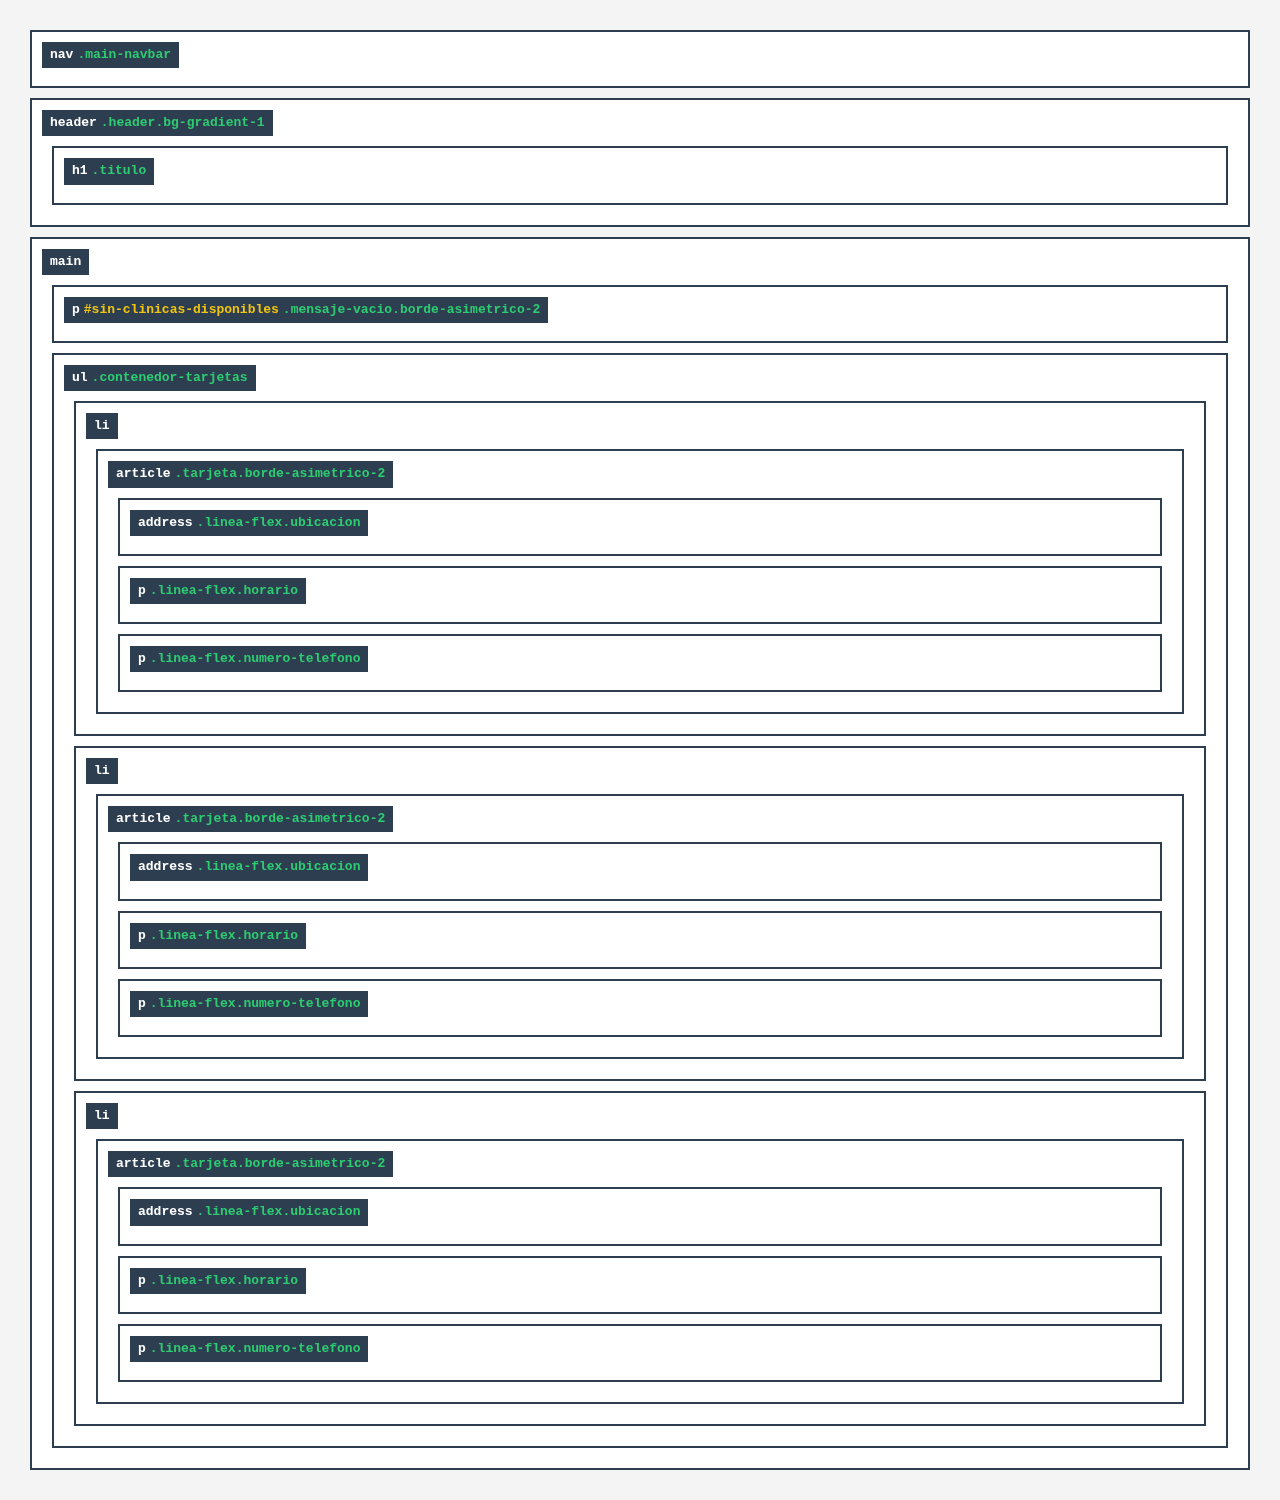
\includegraphics[width=\linewidth,keepaspectratio]{mapasDeEtiquetas/urgencias-boxmodel-new.png}
        \caption{Urgencias (Cambios)}
    \end{minipage}
\end{figure}

\begin{figure}[H]
    \centering
    \begin{minipage}{0.48\textwidth}
        \centering
        
\includegraphics[width=\linewidth,keepaspectratio]{mapasDeEtiquetas/pedir-cita-boxmodel.png}
        \caption{Pedir cita (Base)}
    \end{minipage}\hfill
    \begin{minipage}{0.48\textwidth}
        \centering
        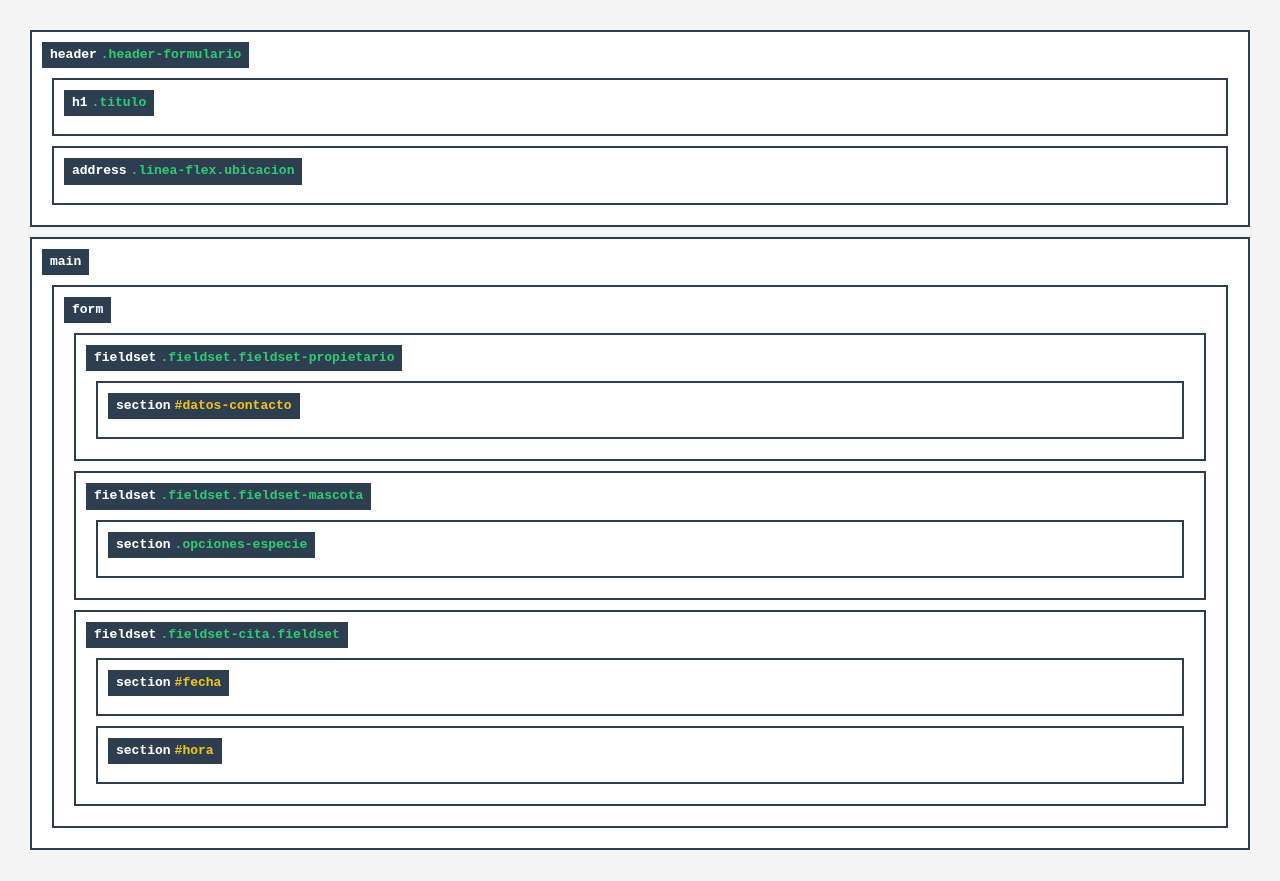
\includegraphics[width=\linewidth,keepaspectratio]{mapasDeEtiquetas/pedir-cita-boxmodel-new.png}
        \caption{Pedir cita (Cambios)}
    \end{minipage}
\end{figure}

\end{document}